% Best-configuration diagnostic suites for the nine MKP instances.
% Include from a document located in paper/ with:
%   % Best-configuration diagnostic suites for the nine MKP instances.
% Include from a document located in paper/ with:
%   % Best-configuration diagnostic suites for the nine MKP instances.
% Include from a document located in paper/ with:
%   % Best-configuration diagnostic suites for the nine MKP instances.
% Include from a document located in paper/ with:
%   \input{mkp_best_diagnostics_EN}
% Required packages: graphicx, subfig (or subcaption with \subfloat redefined).

% Each figure shows the best-performing framework configuration for the
% corresponding instance, selected by highest mean fitness over 31 runs.
% DTW--3K is best for mknapcb1 and mknapcb3--mknapcb8;
% DDTW--3K is best for mknapcb2 and mknapcb9.

Figures~\ref{fig:mkp-best-cb1}--\ref{fig:mkp-best-cb9} present the
diagnostic suite for each of the nine Chu--Beasley MKP instances under its
best-performing framework configuration, selected by highest mean fitness
over the 31 runs, with corresponding executions treated as paired. DTW with $T_{\max}=3{,}000$ achieved the
highest mean in seven instances (mknapcb1 and mknapcb3--mknapcb8), while
DDTW with $T_{\max}=3{,}000$ was superior for mknapcb2 and mknapcb9.
Each figure comprises three panels: (a)~a box-plot comparing the
final-fitness distributions of the hybrid framework against the standalone
metaheuristics over the 31 runs, allowing visual assessment of both central
tendency and dispersion; (b)~the convergence trajectory of the best run,
showing the evolution of the incumbent fitness along with the solver
transitions triggered by the stagnation monitor; and (c)~the elastic
warping profile $\Delta = D_1 - D_2$, where positive values indicate
detected stagnation phases and negative values correspond to periods of
active improvement.

% --- mknapcb1: DTW, 3,000 iterations ---
\begin{figure}[htbp]
\centering
\subfloat[Metaheuristic comparison.]{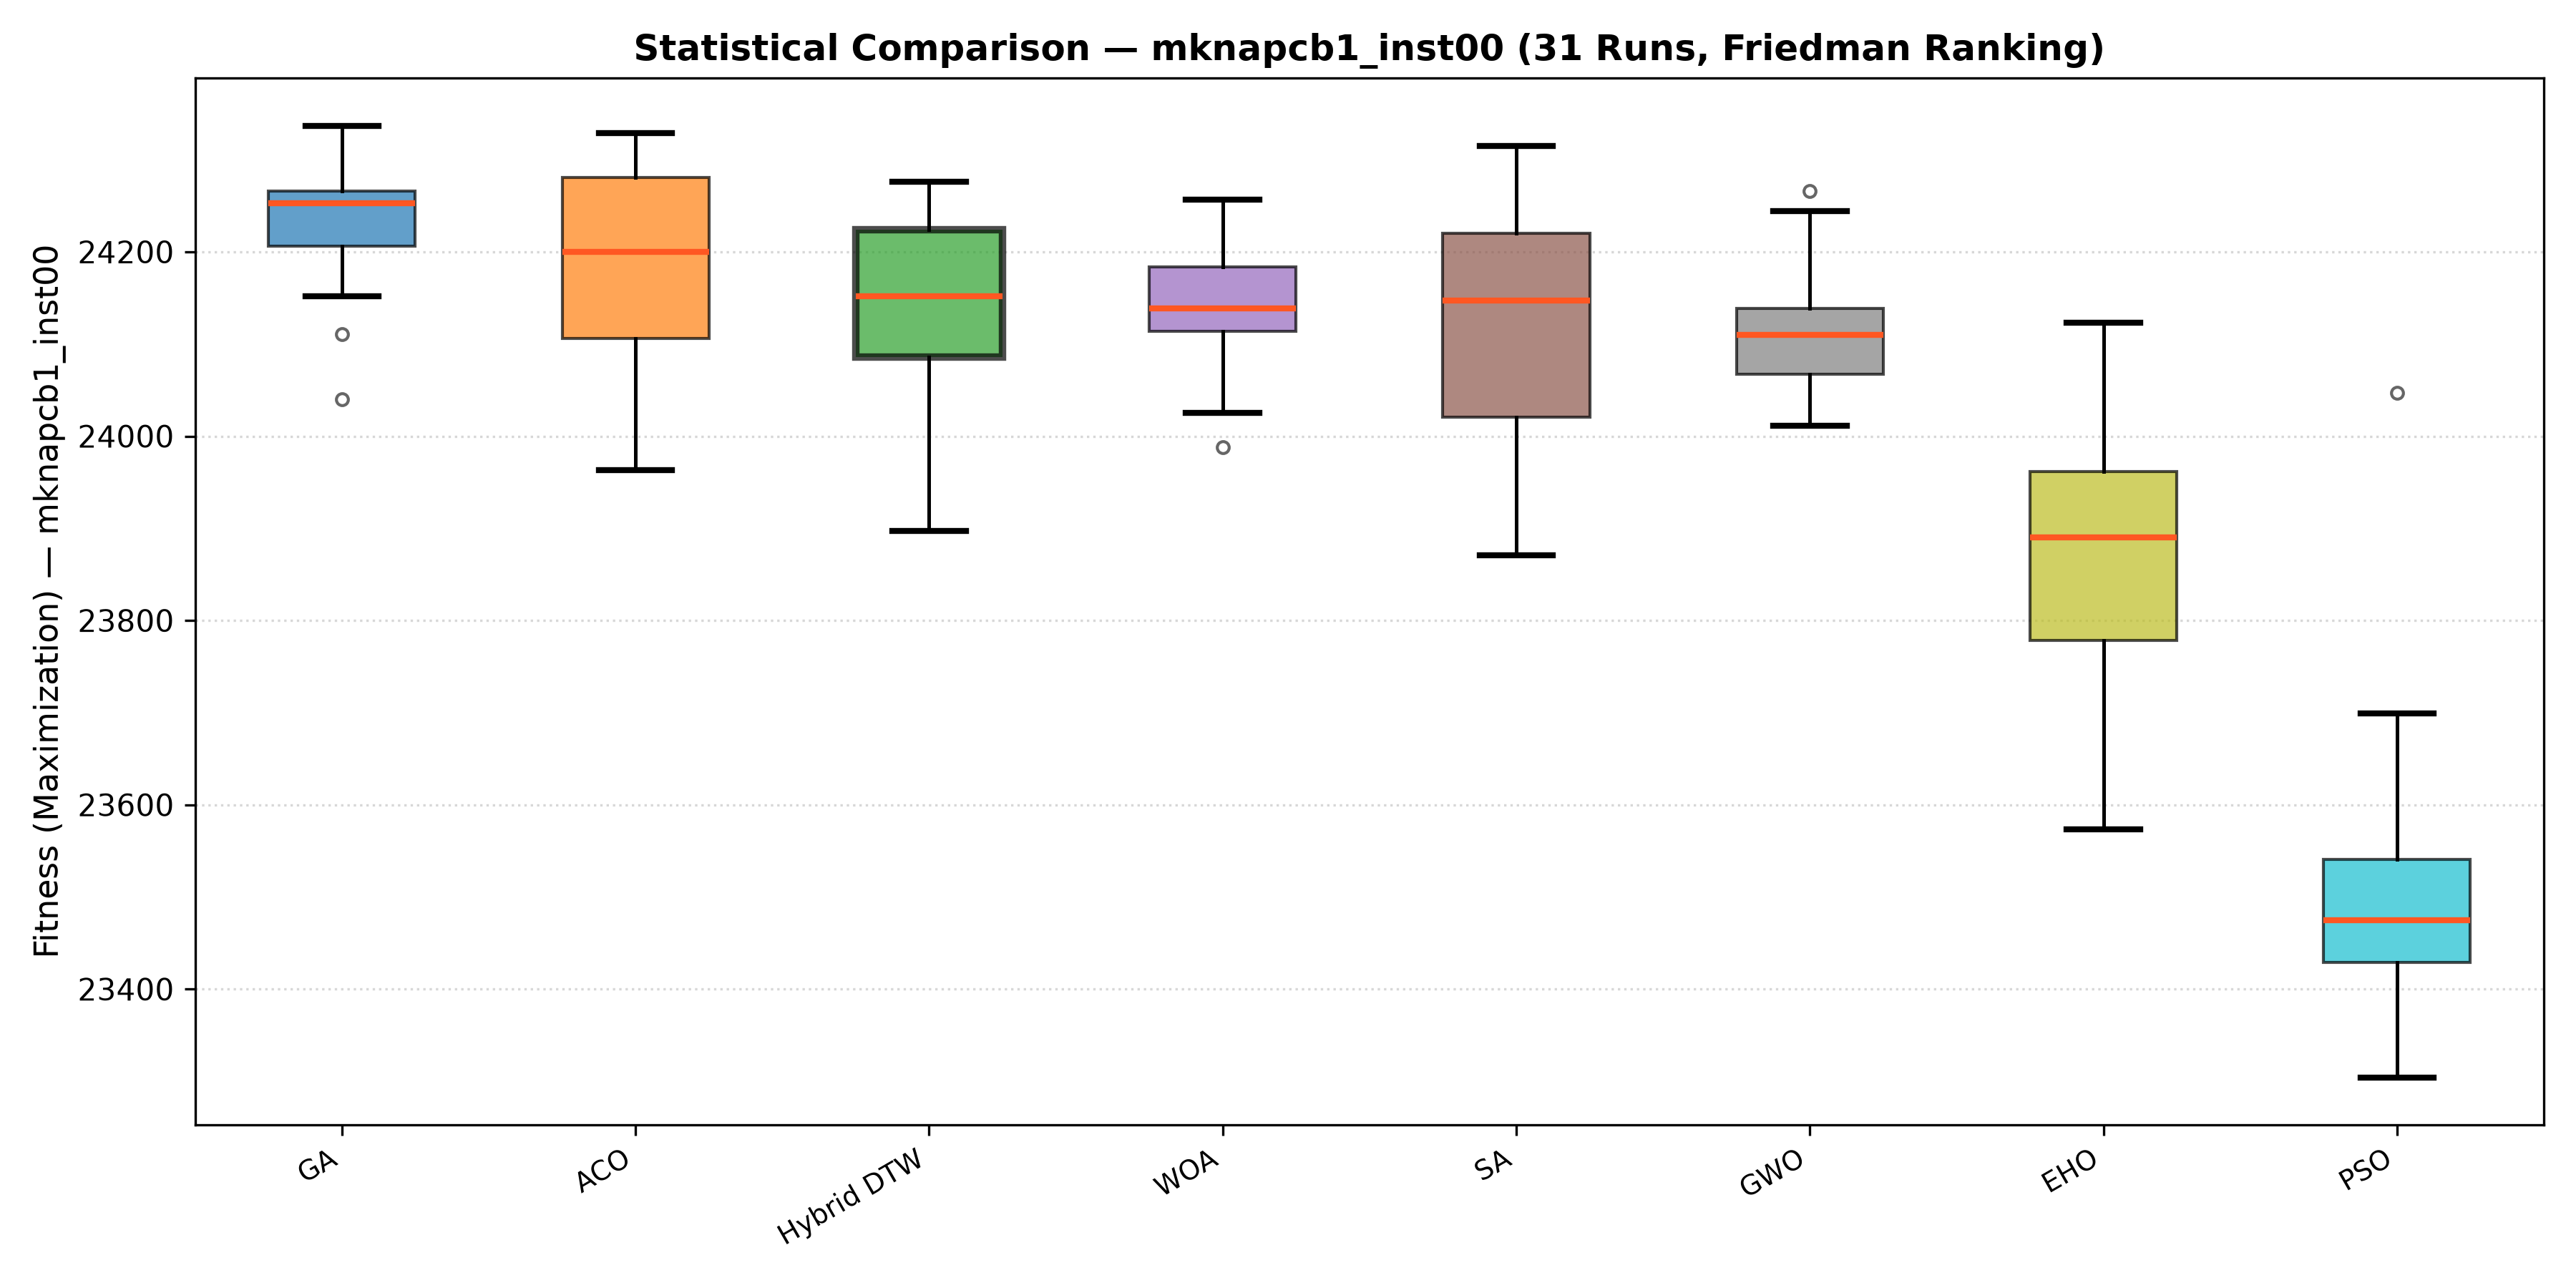
\includegraphics[width=0.32\textwidth]{imagenes_paper/mkp_dtw_3k_mknapcb1_comparativo_mh.png}}\hfill
\subfloat[Best-run convergence.]{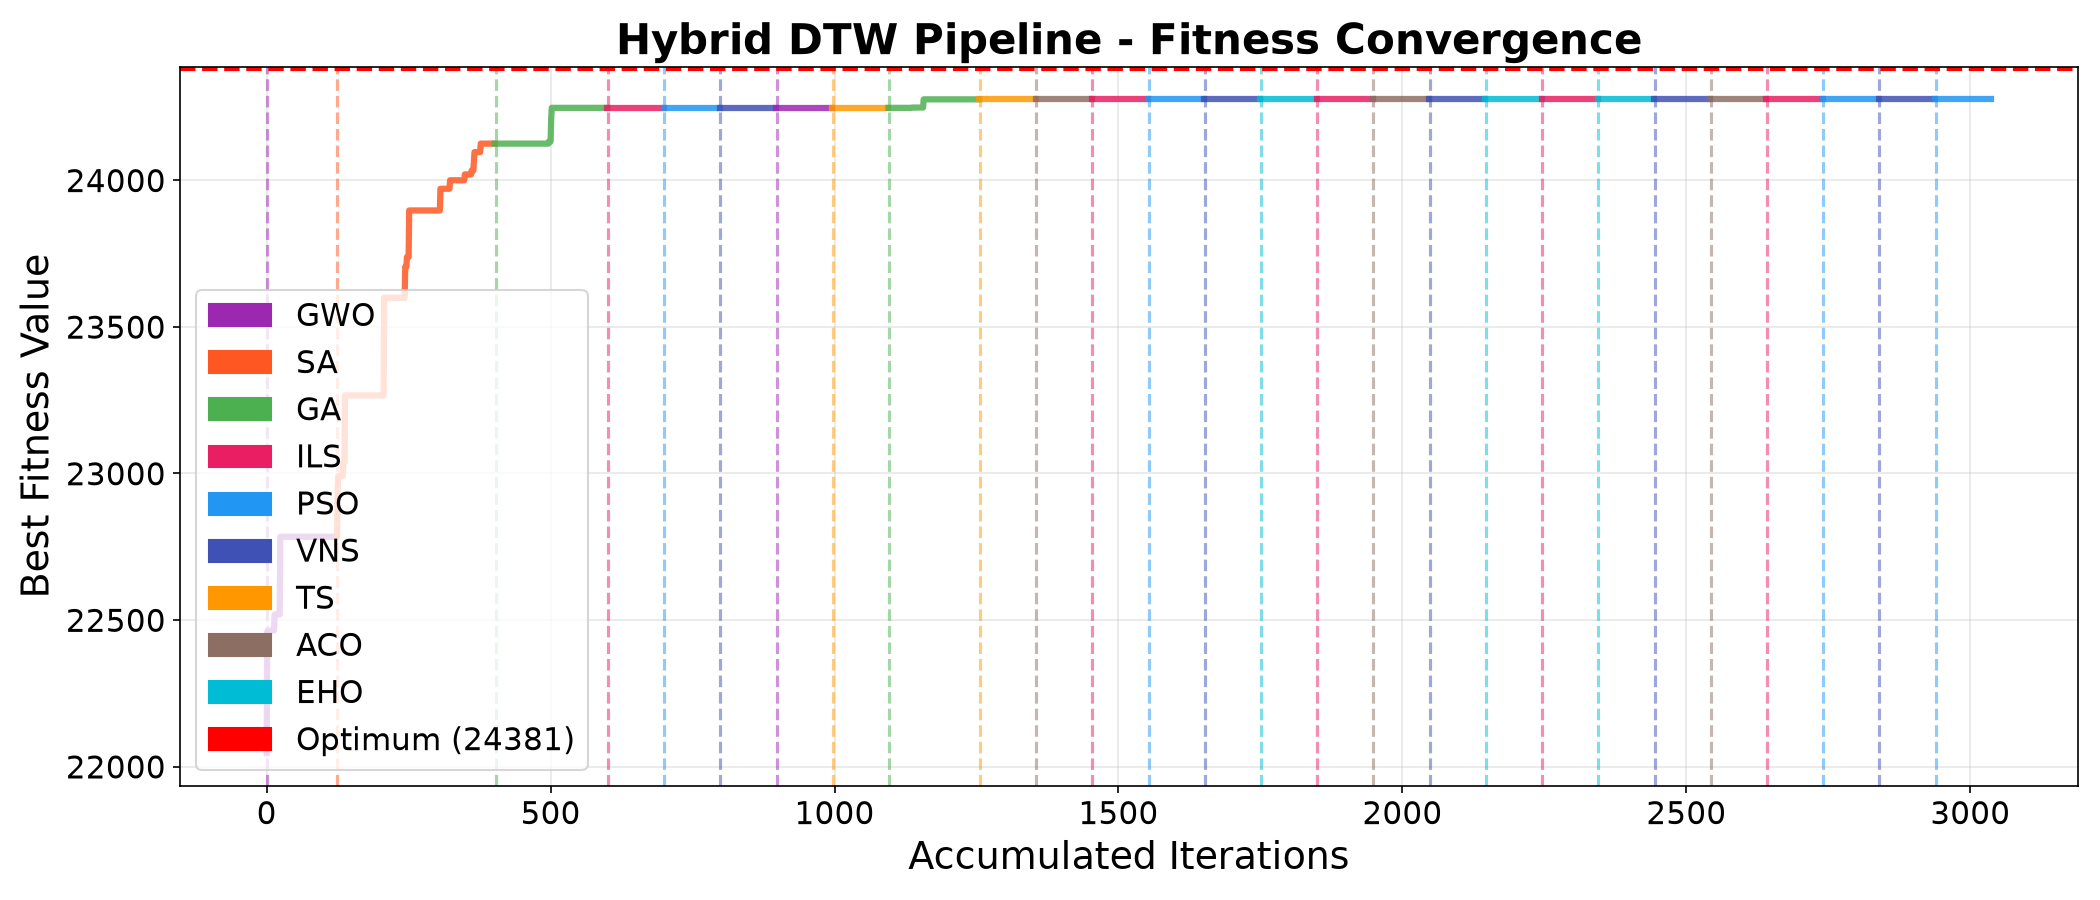
\includegraphics[width=0.32\textwidth]{imagenes_paper/mkp_dtw_3k_mknapcb1_convergencia.png}}\hfill
\subfloat[Elastic metric $\Delta=D_1-D_2$.]{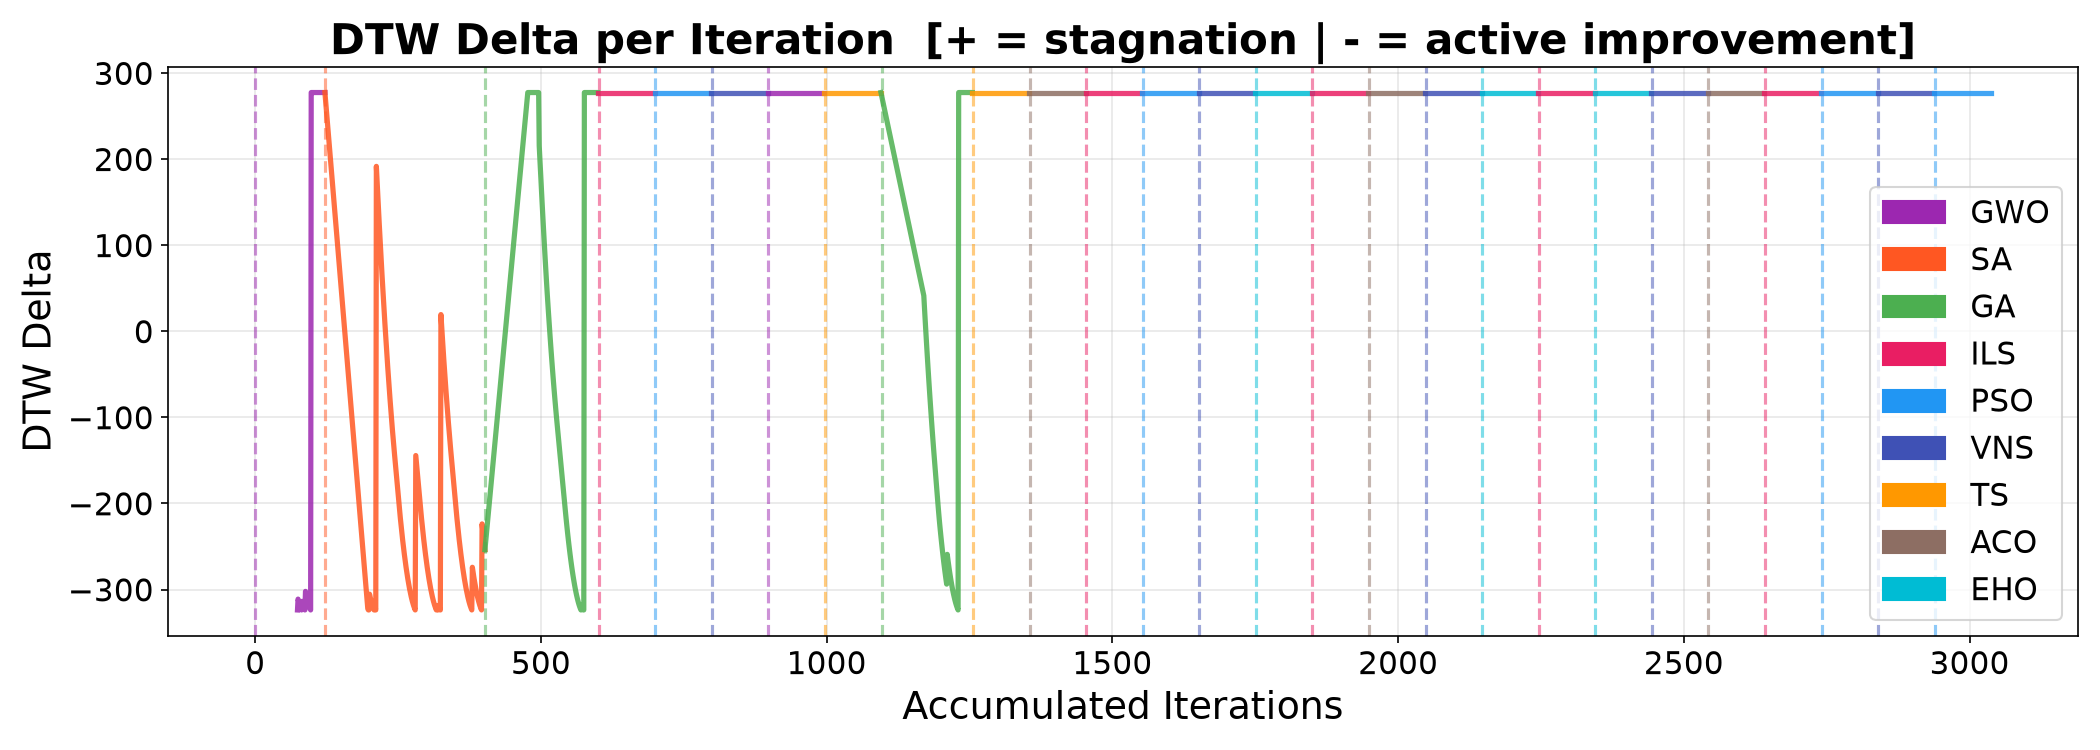
\includegraphics[width=0.32\textwidth]{imagenes_paper/mkp_dtw_3k_mknapcb1_delta.png}}
\caption{Diagnostic suite for instance \textbf{mknapcb1} ($n=100$, $m=5$) under the DTW framework with $T_{\max}=3{,}000$: (a)~final-fitness distribution over $N=31$ runs; (b)~convergence trajectory of the best run; (c)~elastic warping profile $\Delta$.}
\label{fig:mkp-best-cb1}
\end{figure}

% --- mknapcb2: DDTW, 3,000 iterations ---
\begin{figure}[htbp]
\centering
\subfloat[Metaheuristic comparison.]{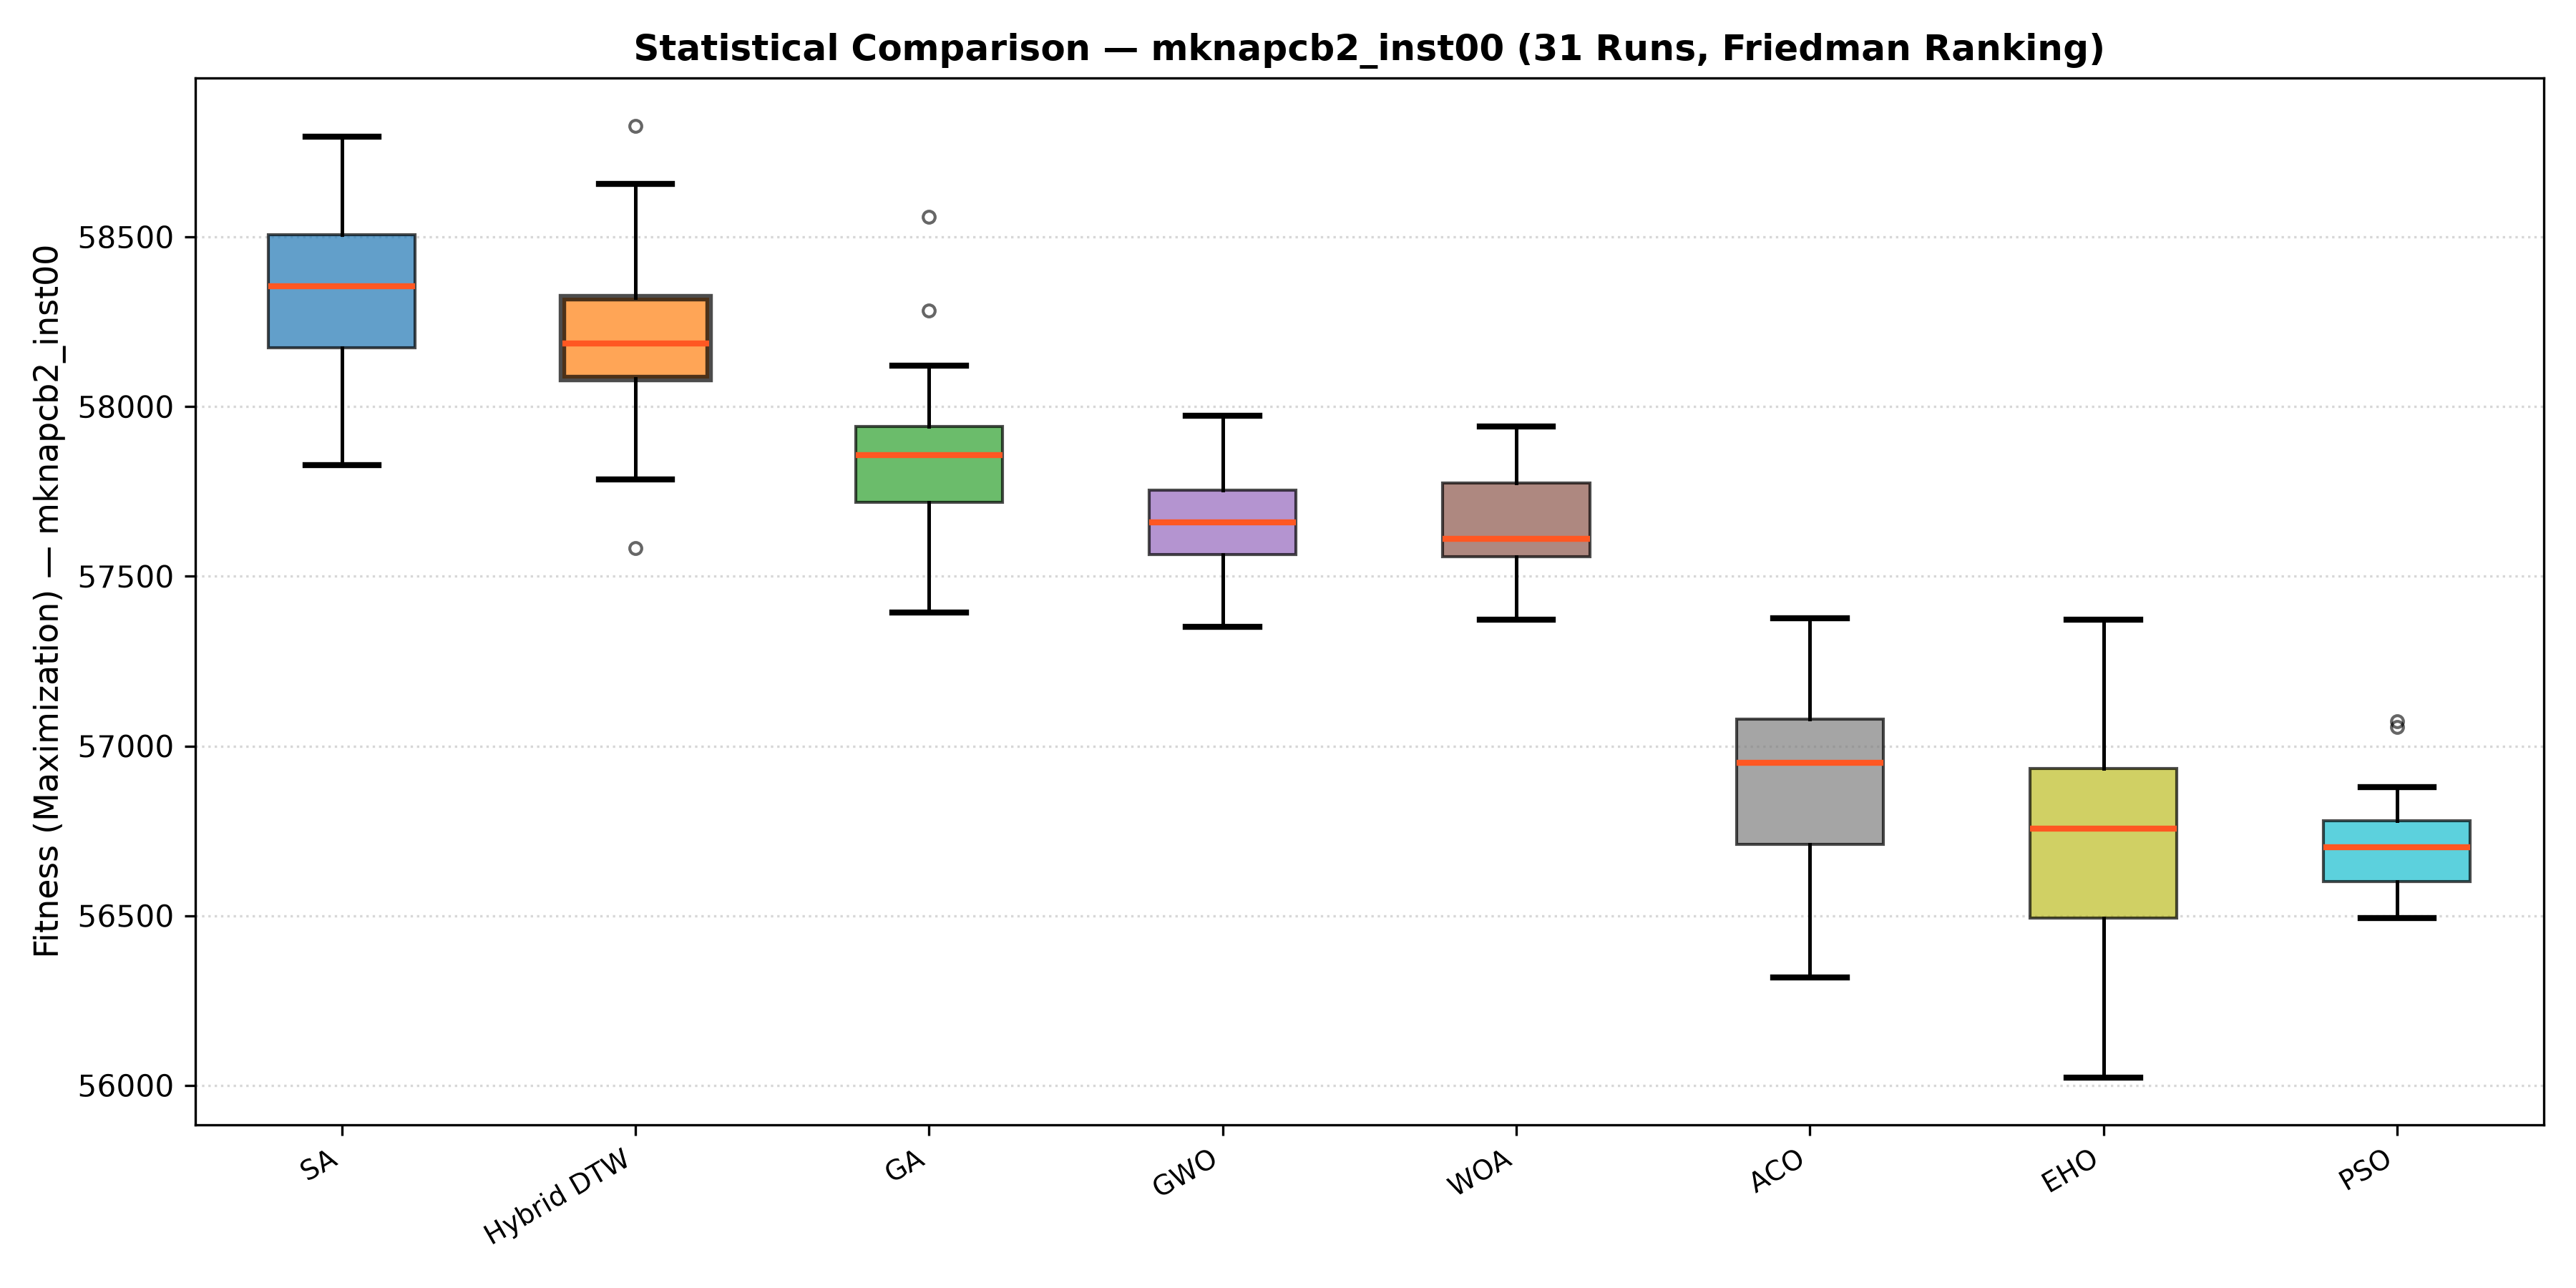
\includegraphics[width=0.32\textwidth]{imagenes_paper/mkp_ddtw_3k_mknapcb2_comparativo_mh.png}}\hfill
\subfloat[Best-run convergence.]{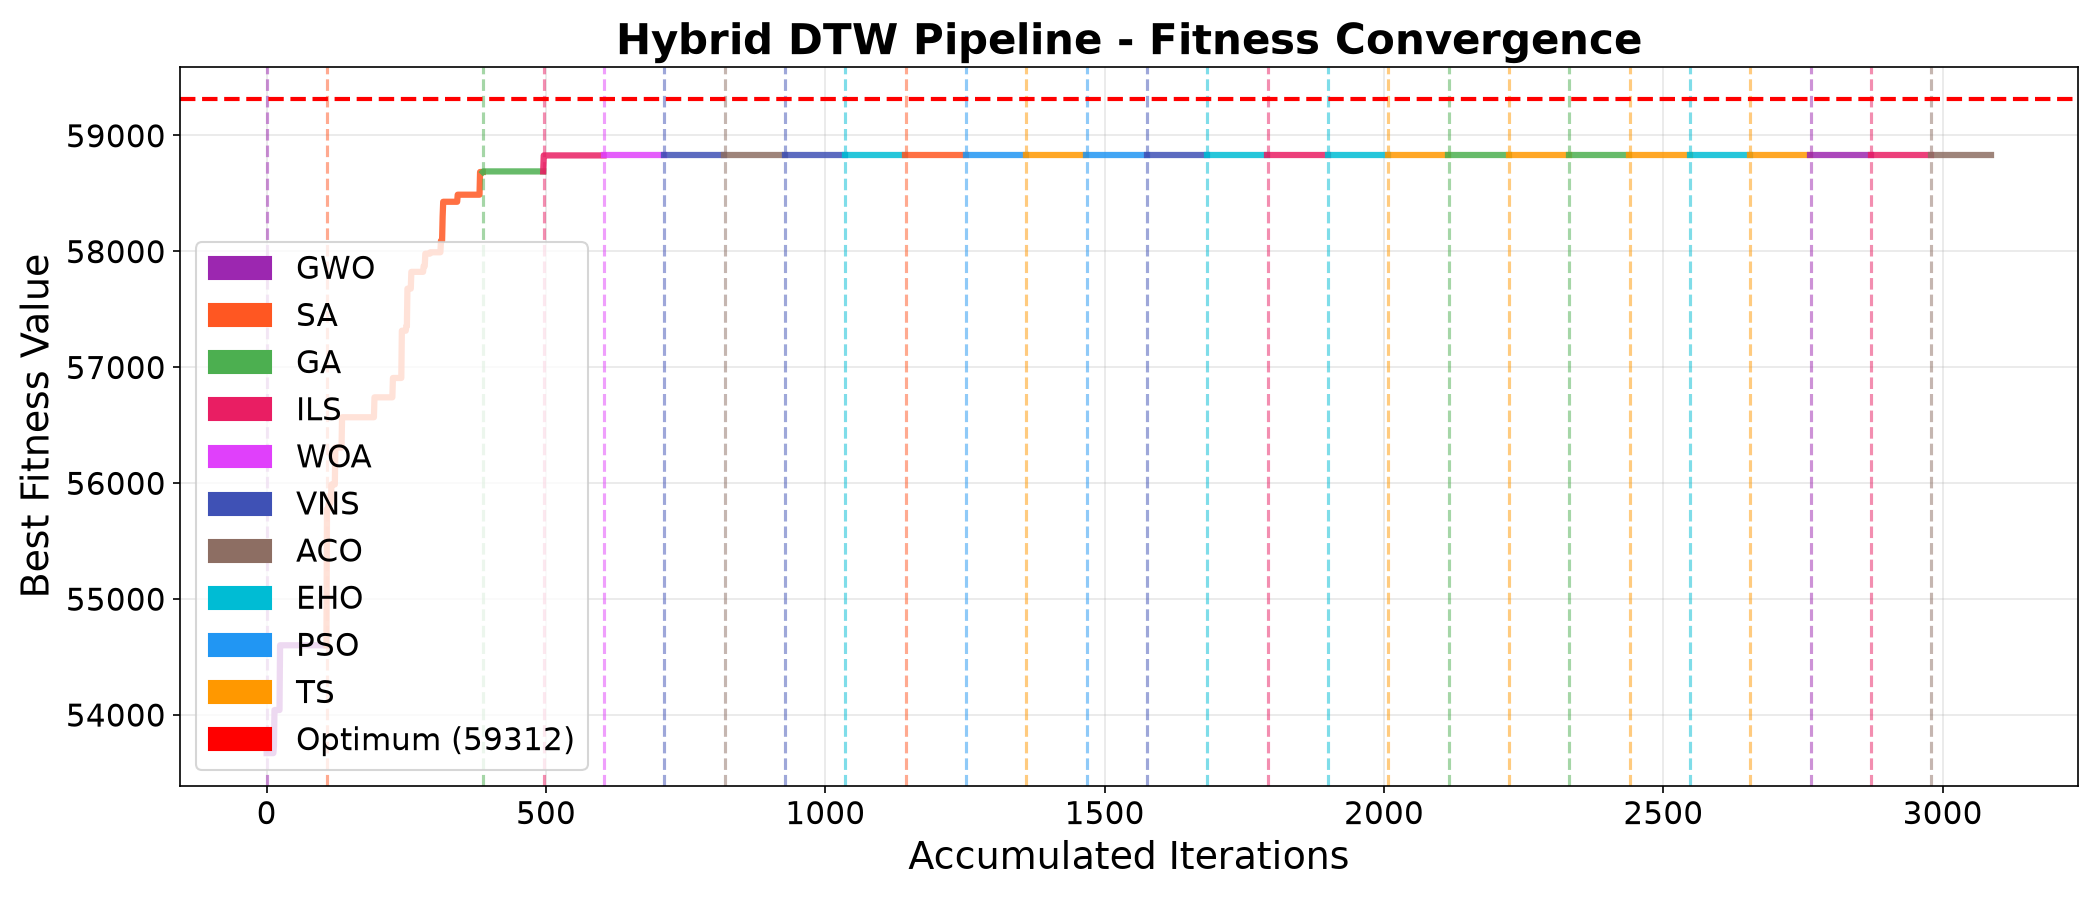
\includegraphics[width=0.32\textwidth]{imagenes_paper/mkp_ddtw_3k_mknapcb2_convergencia.png}}\hfill
\subfloat[Elastic metric $\Delta=D_1-D_2$.]{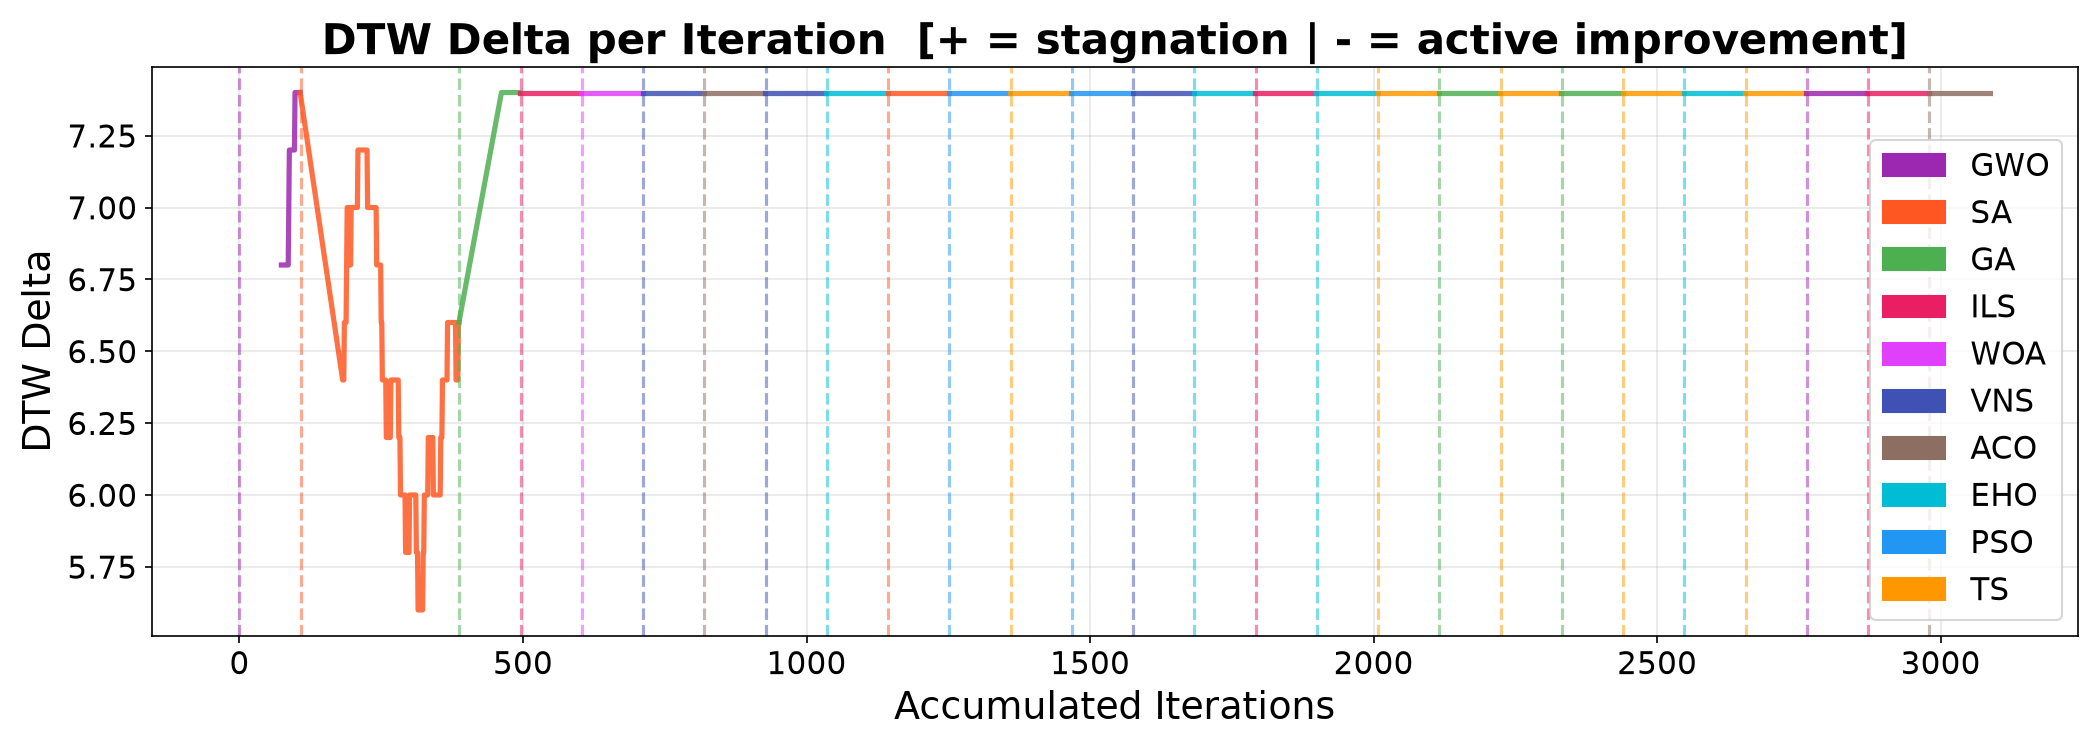
\includegraphics[width=0.32\textwidth]{imagenes_paper/mkp_ddtw_3k_mknapcb2_delta.png}}
\caption{Diagnostic suite for instance \textbf{mknapcb2} ($n=250$, $m=5$) under the DDTW framework with $T_{\max}=3{,}000$: (a)~final-fitness distribution over $N=31$ runs; (b)~convergence trajectory of the best run; (c)~elastic warping profile $\Delta$.}
\label{fig:mkp-best-cb2}
\end{figure}

% --- mknapcb3: DTW, 3,000 iterations ---
\begin{figure}[htbp]
\centering
\subfloat[Metaheuristic comparison.]{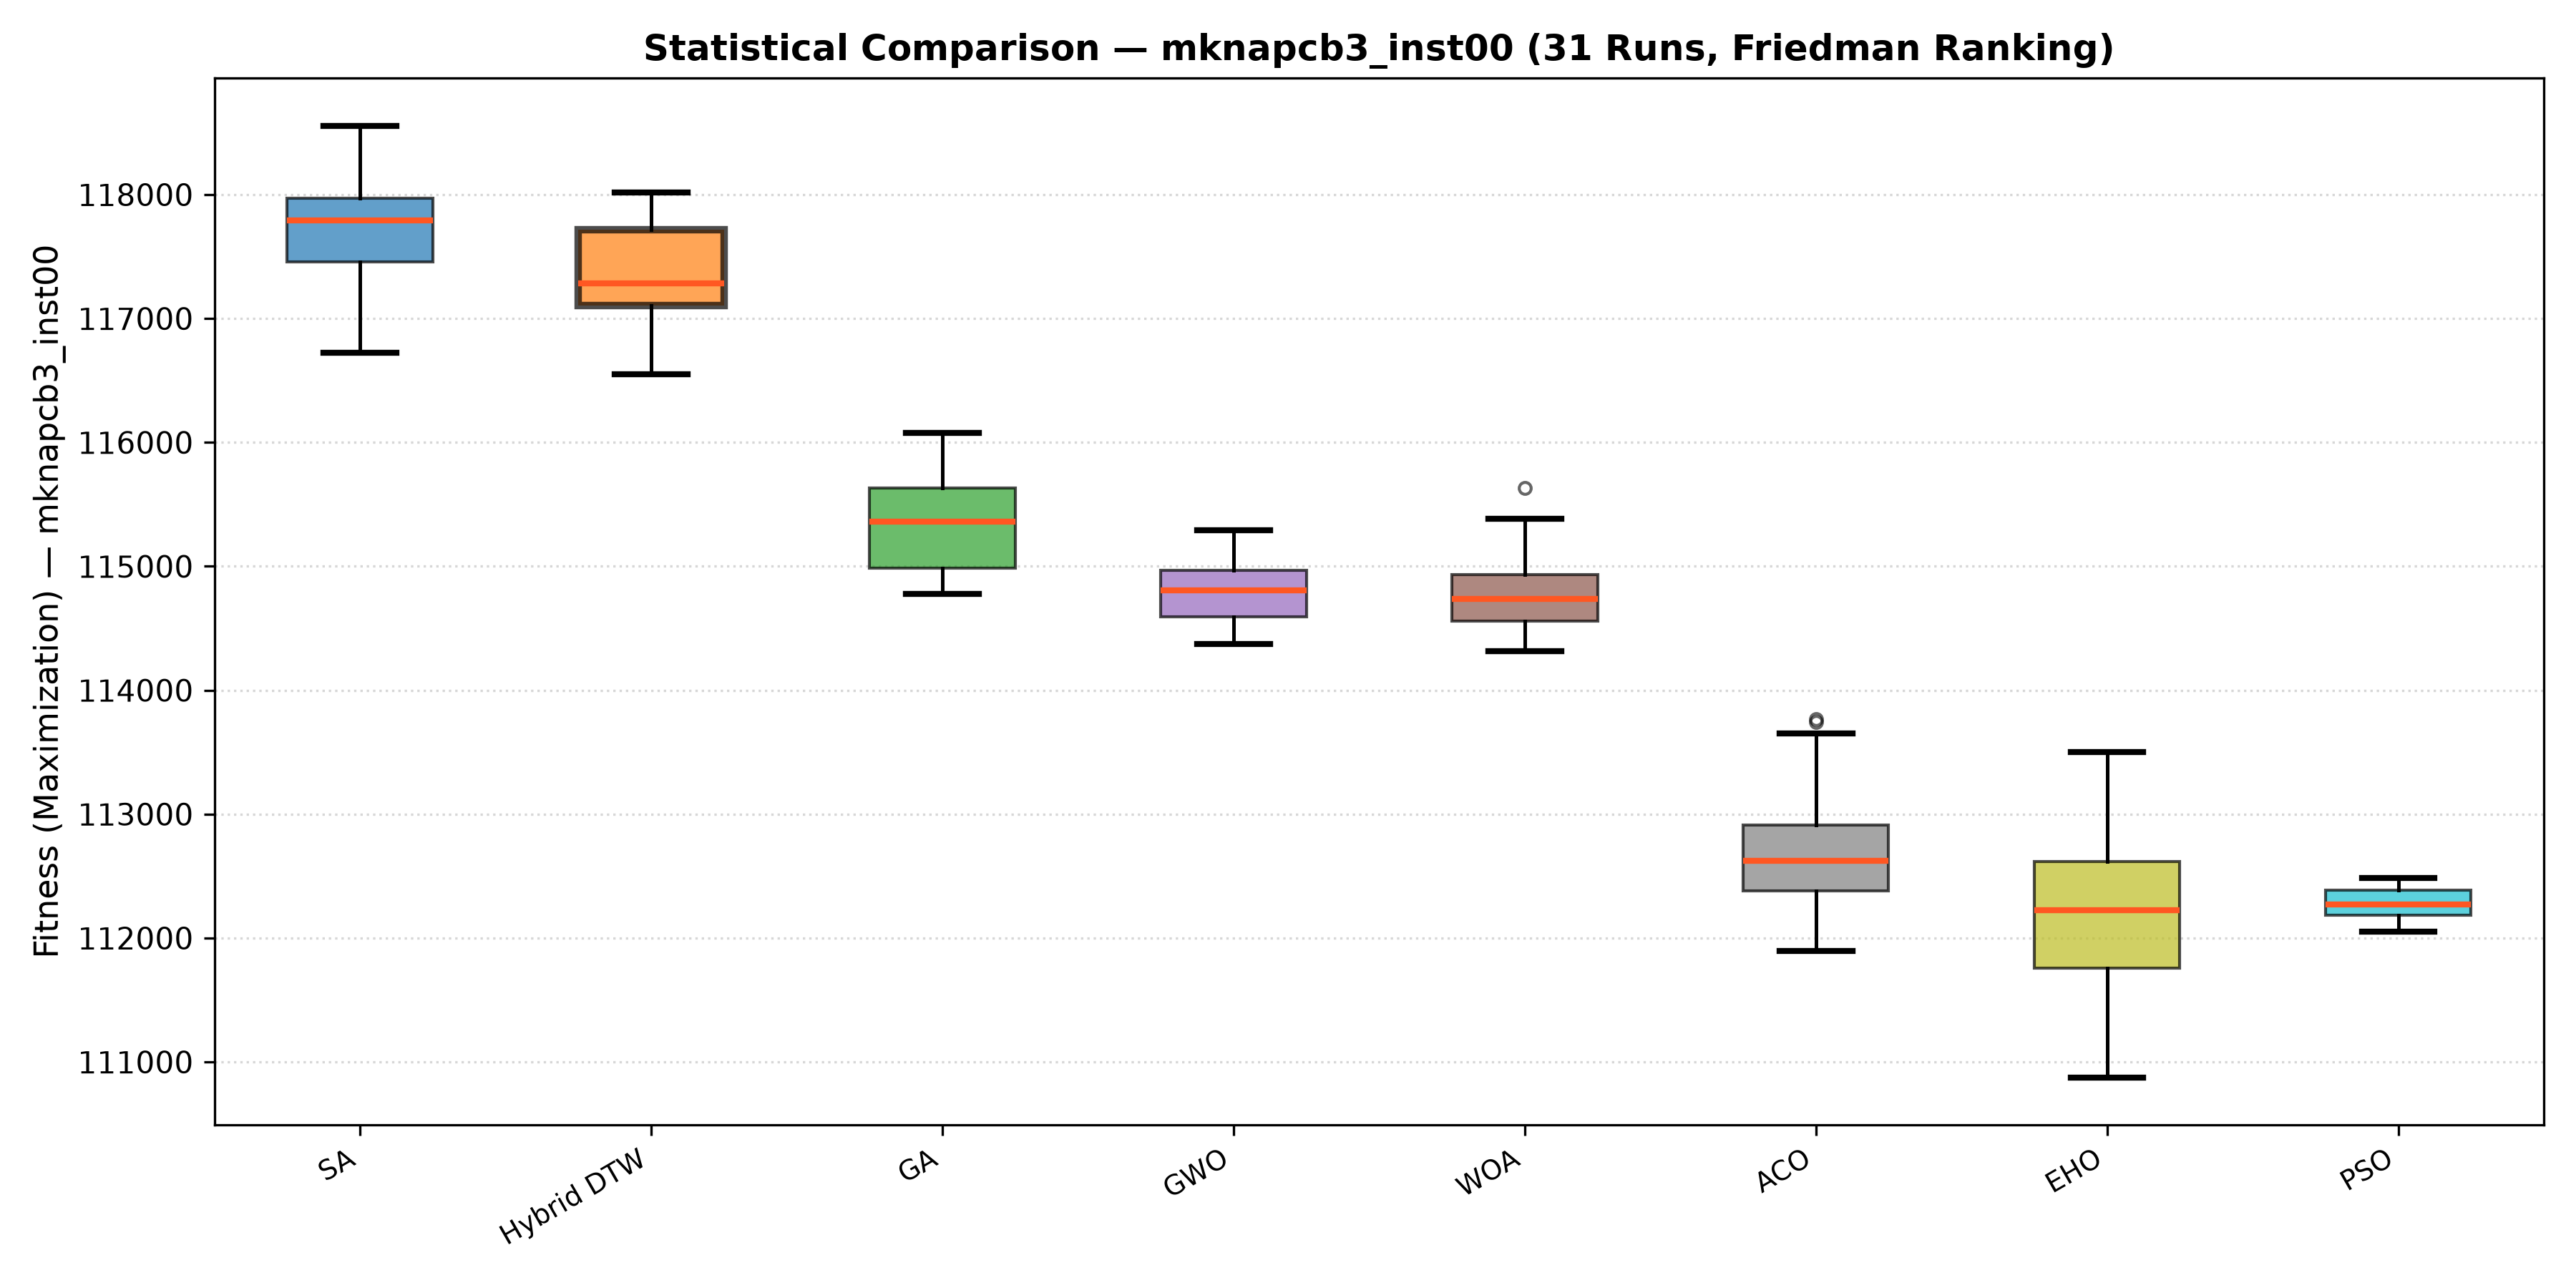
\includegraphics[width=0.32\textwidth]{imagenes_paper/mkp_dtw_3k_mknapcb3_comparativo_mh.png}}\hfill
\subfloat[Best-run convergence.]{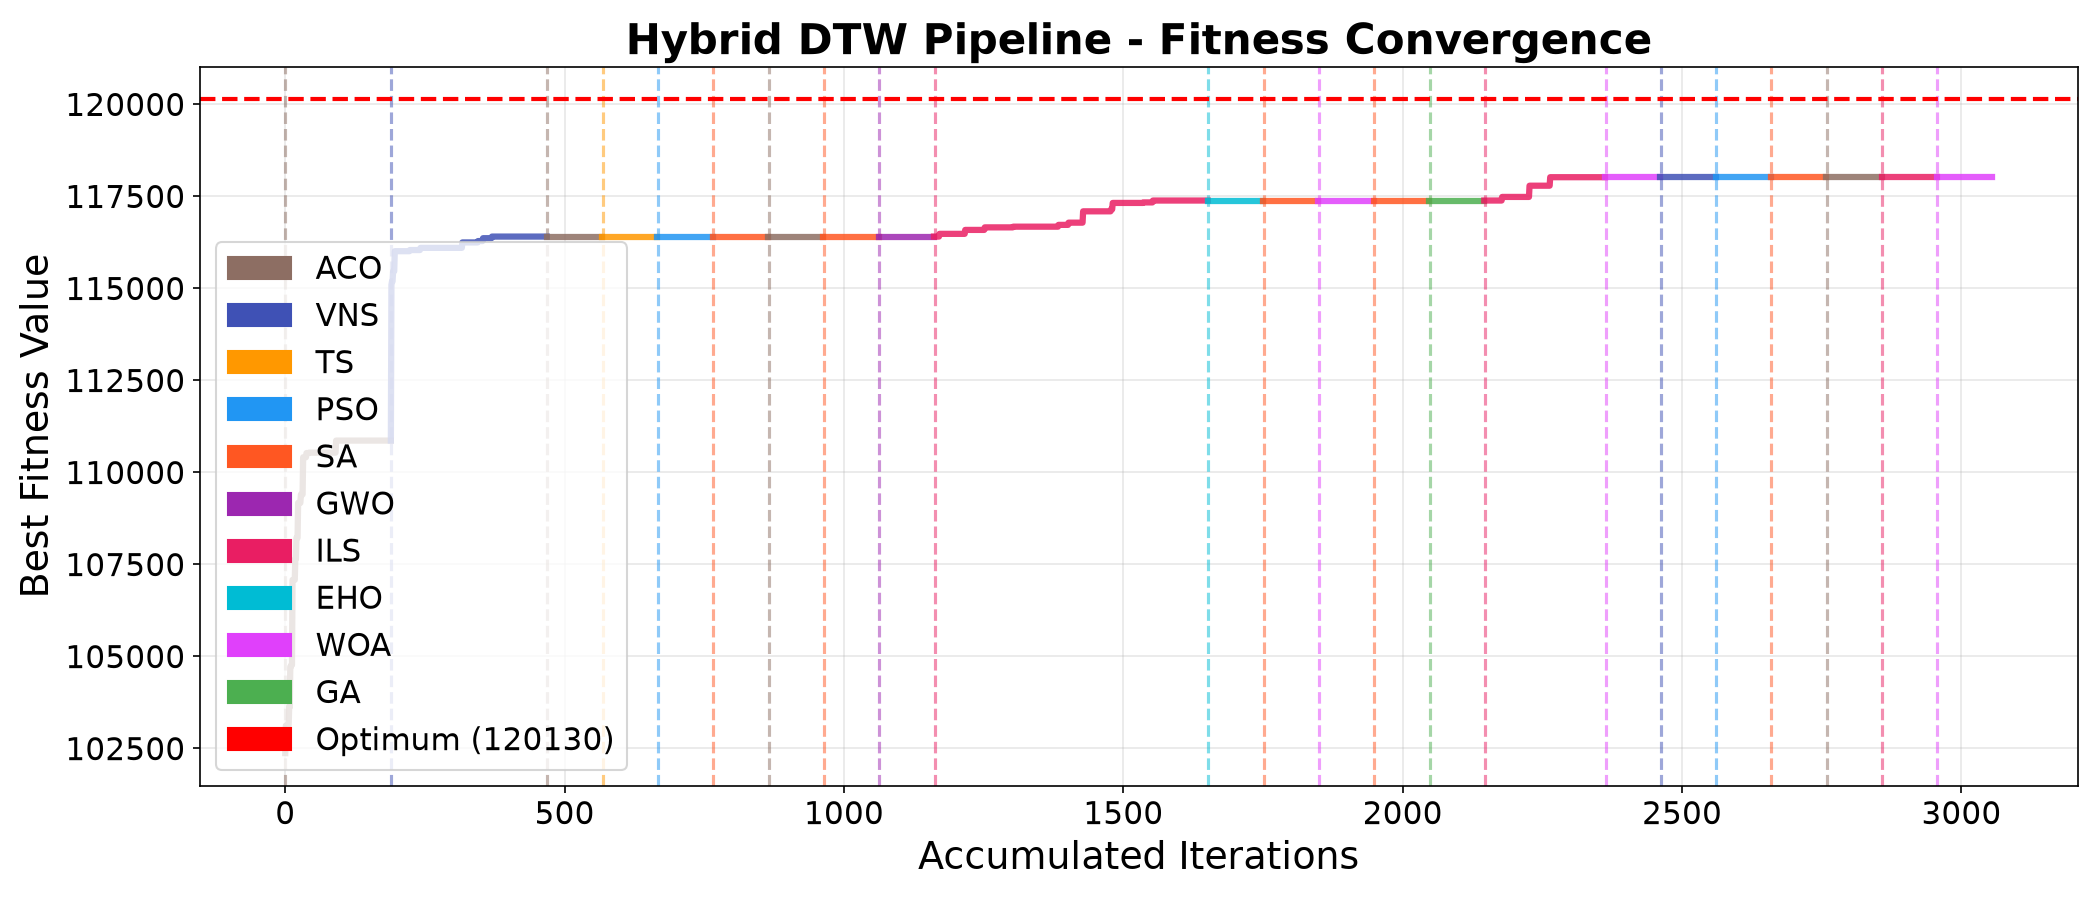
\includegraphics[width=0.32\textwidth]{imagenes_paper/mkp_dtw_3k_mknapcb3_convergencia.png}}\hfill
\subfloat[Elastic metric $\Delta=D_1-D_2$.]{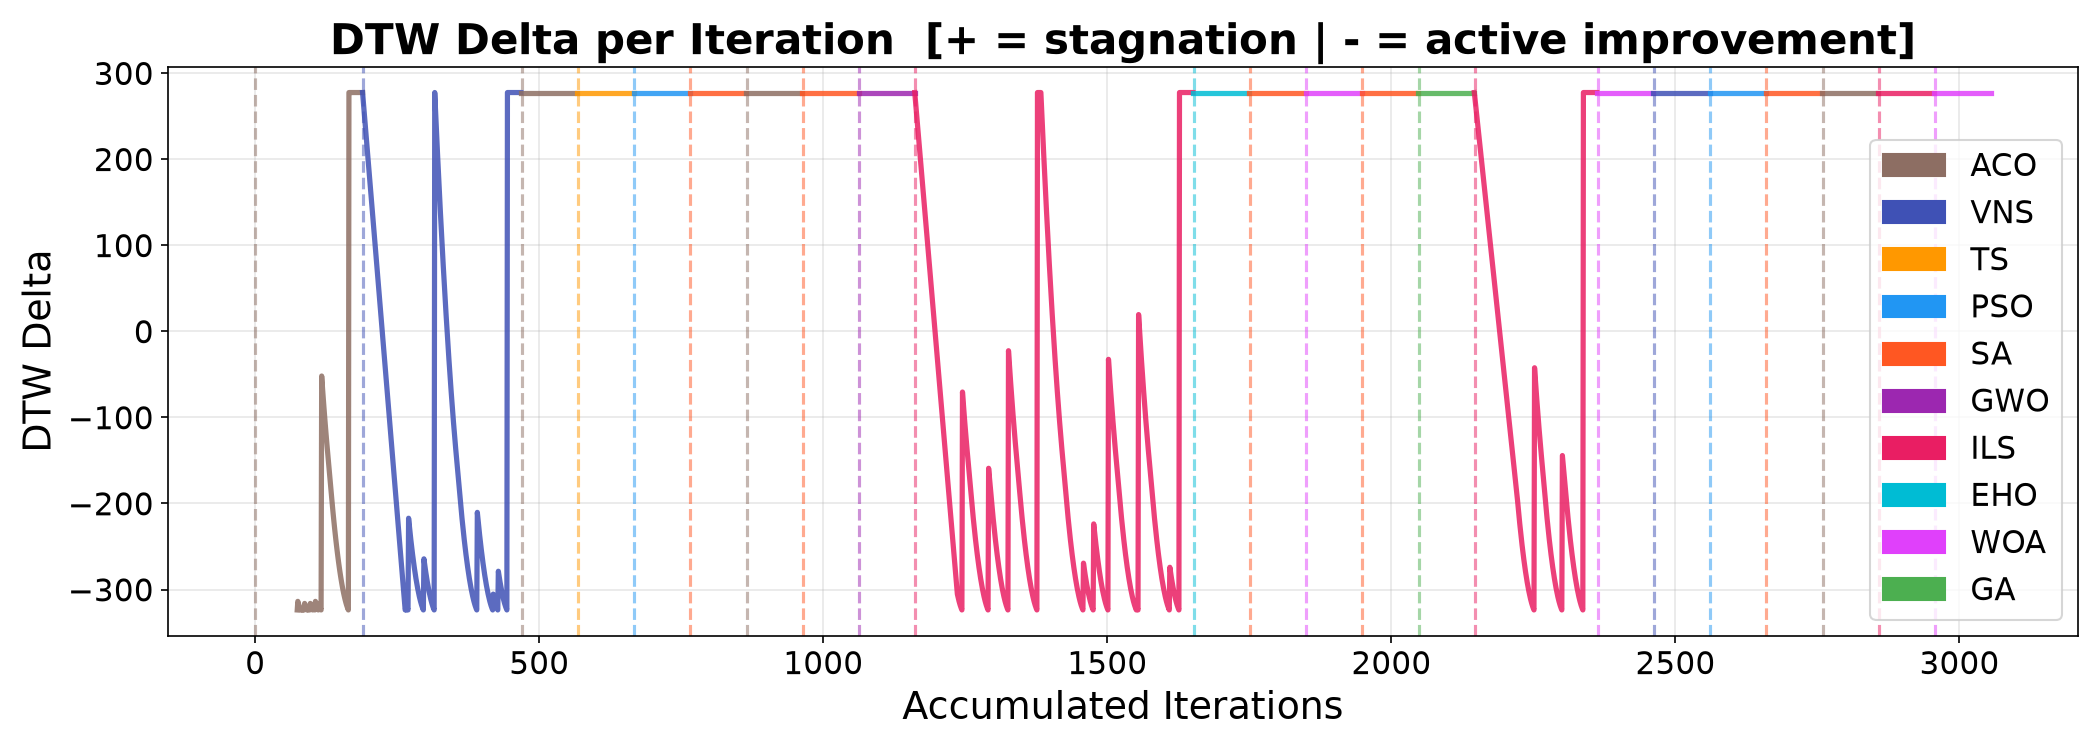
\includegraphics[width=0.32\textwidth]{imagenes_paper/mkp_dtw_3k_mknapcb3_delta.png}}
\caption{Diagnostic suite for instance \textbf{mknapcb3} ($n=500$, $m=5$) under the DTW framework with $T_{\max}=3{,}000$: (a)~final-fitness distribution over $N=31$ runs; (b)~convergence trajectory of the best run; (c)~elastic warping profile $\Delta$.}
\label{fig:mkp-best-cb3}
\end{figure}

% --- mknapcb4: DTW, 3,000 iterations ---
\begin{figure}[htbp]
\centering
\subfloat[Metaheuristic comparison.]{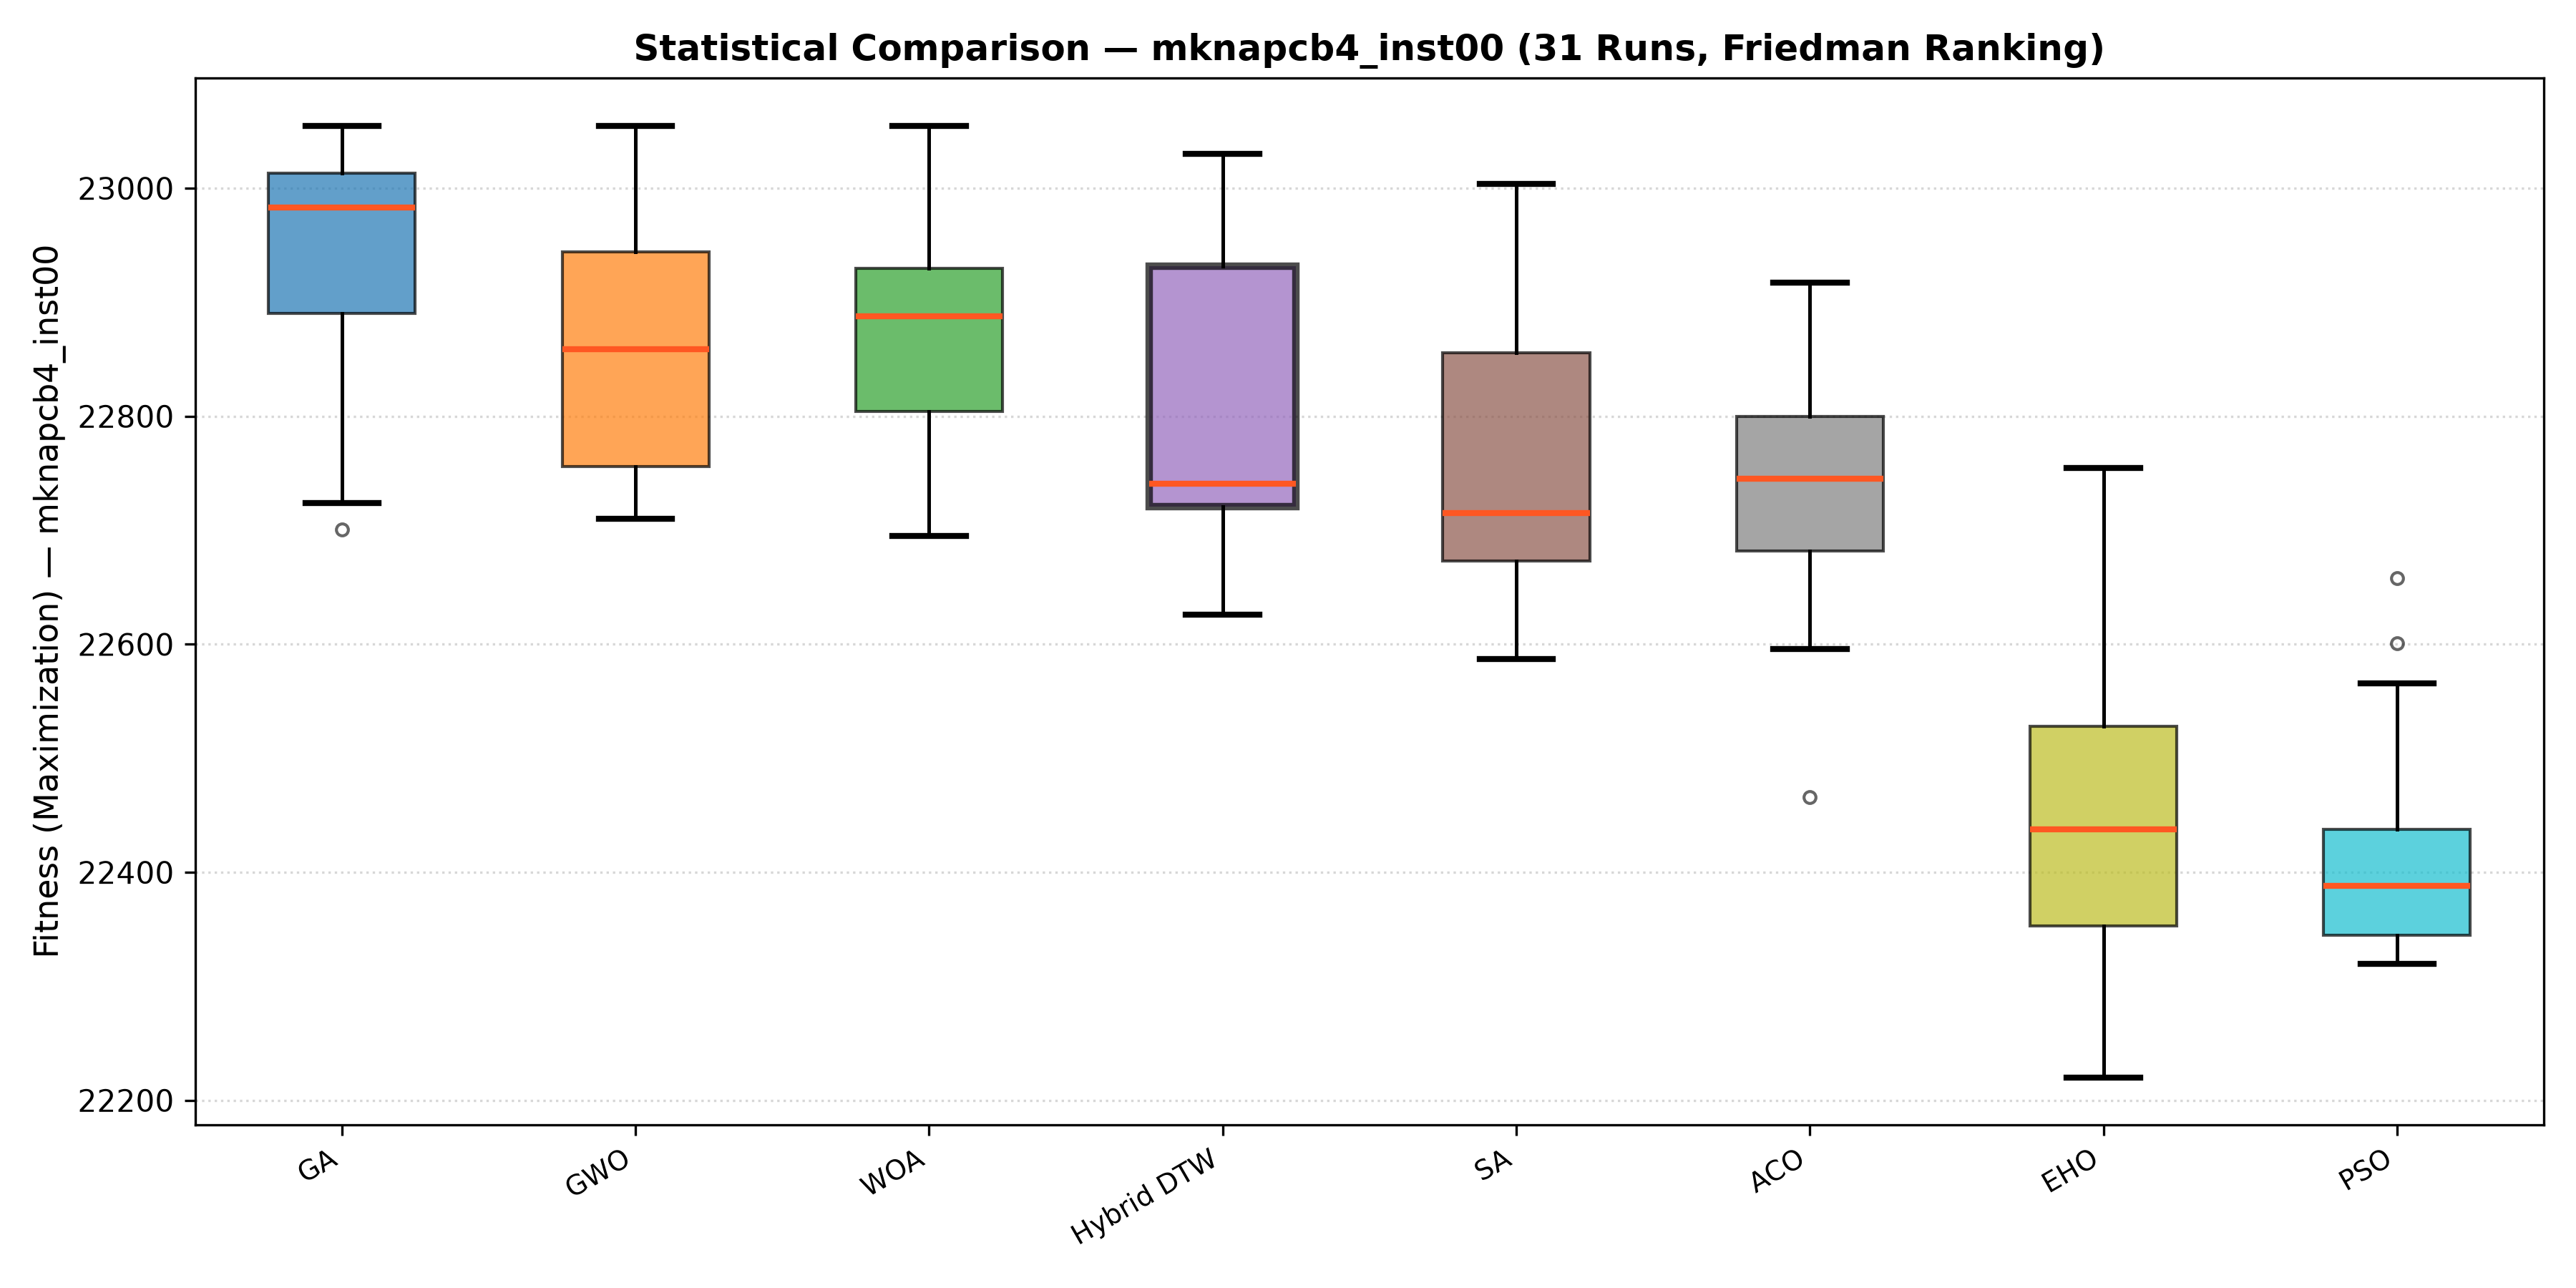
\includegraphics[width=0.32\textwidth]{imagenes_paper/mkp_dtw_3k_mknapcb4_comparativo_mh.png}}\hfill
\subfloat[Best-run convergence.]{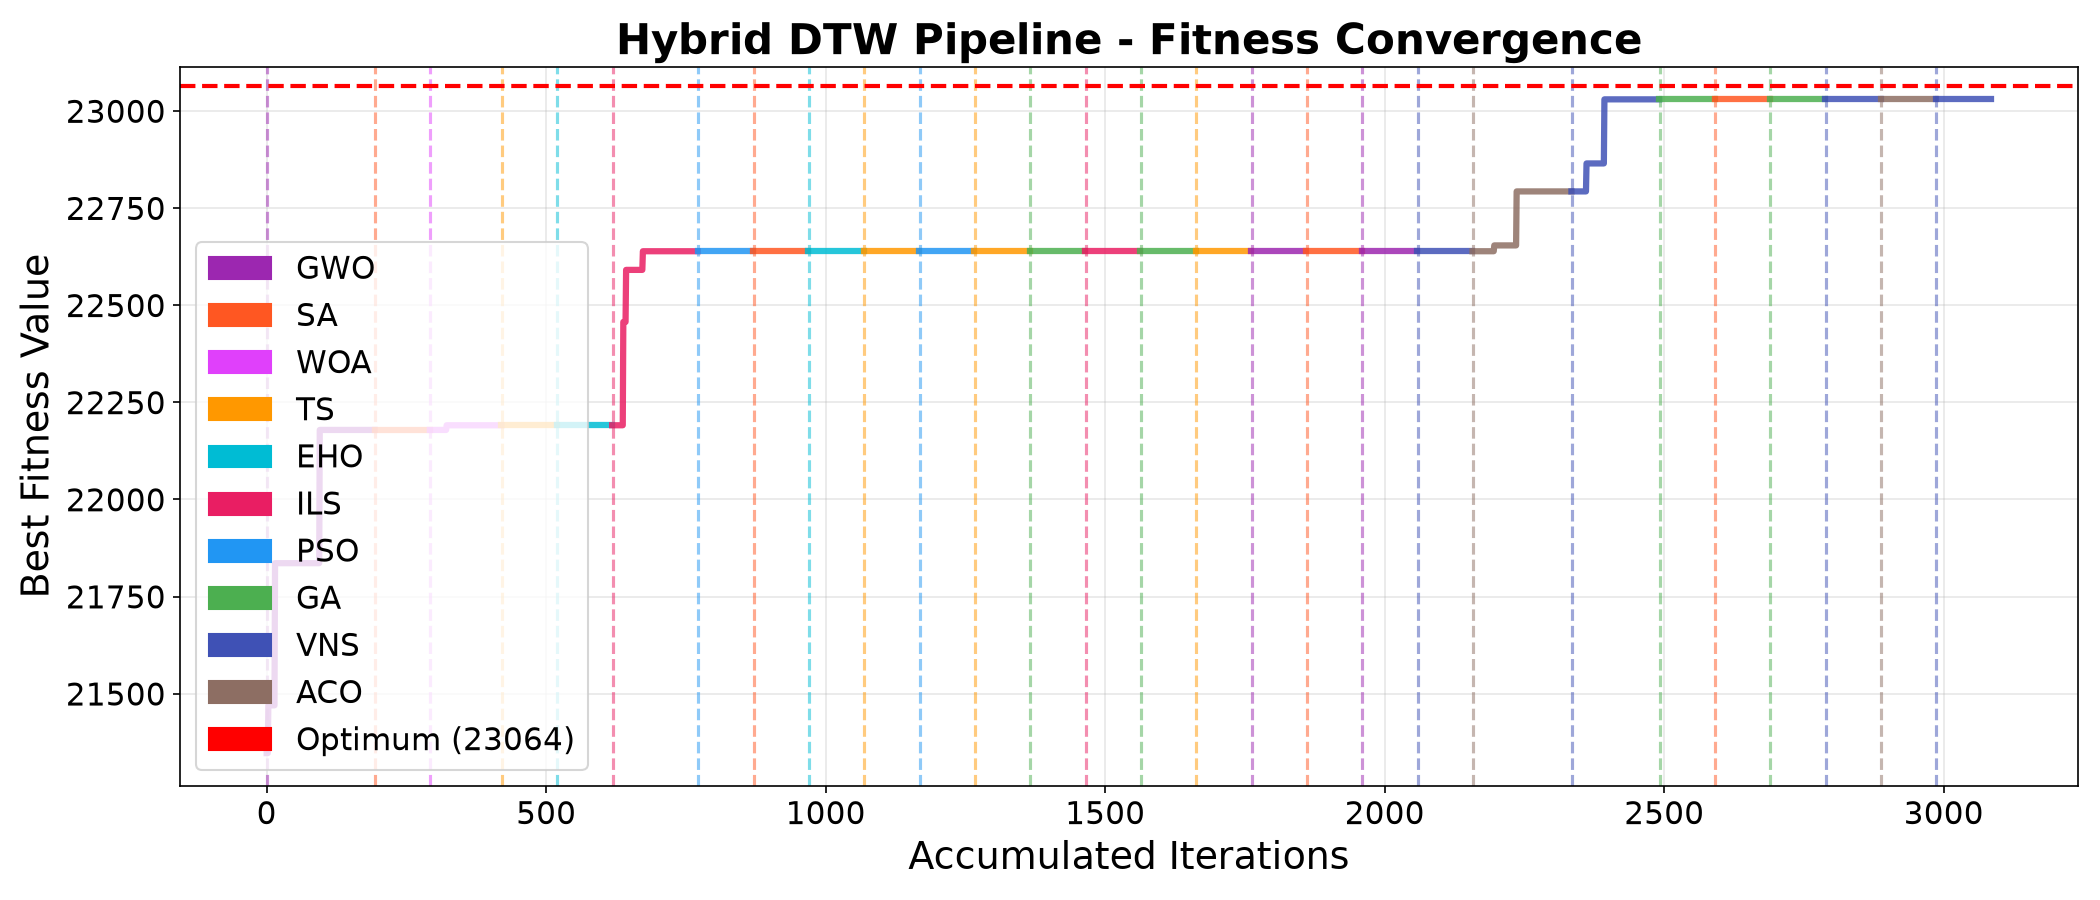
\includegraphics[width=0.32\textwidth]{imagenes_paper/mkp_dtw_3k_mknapcb4_convergencia.png}}\hfill
\subfloat[Elastic metric $\Delta=D_1-D_2$.]{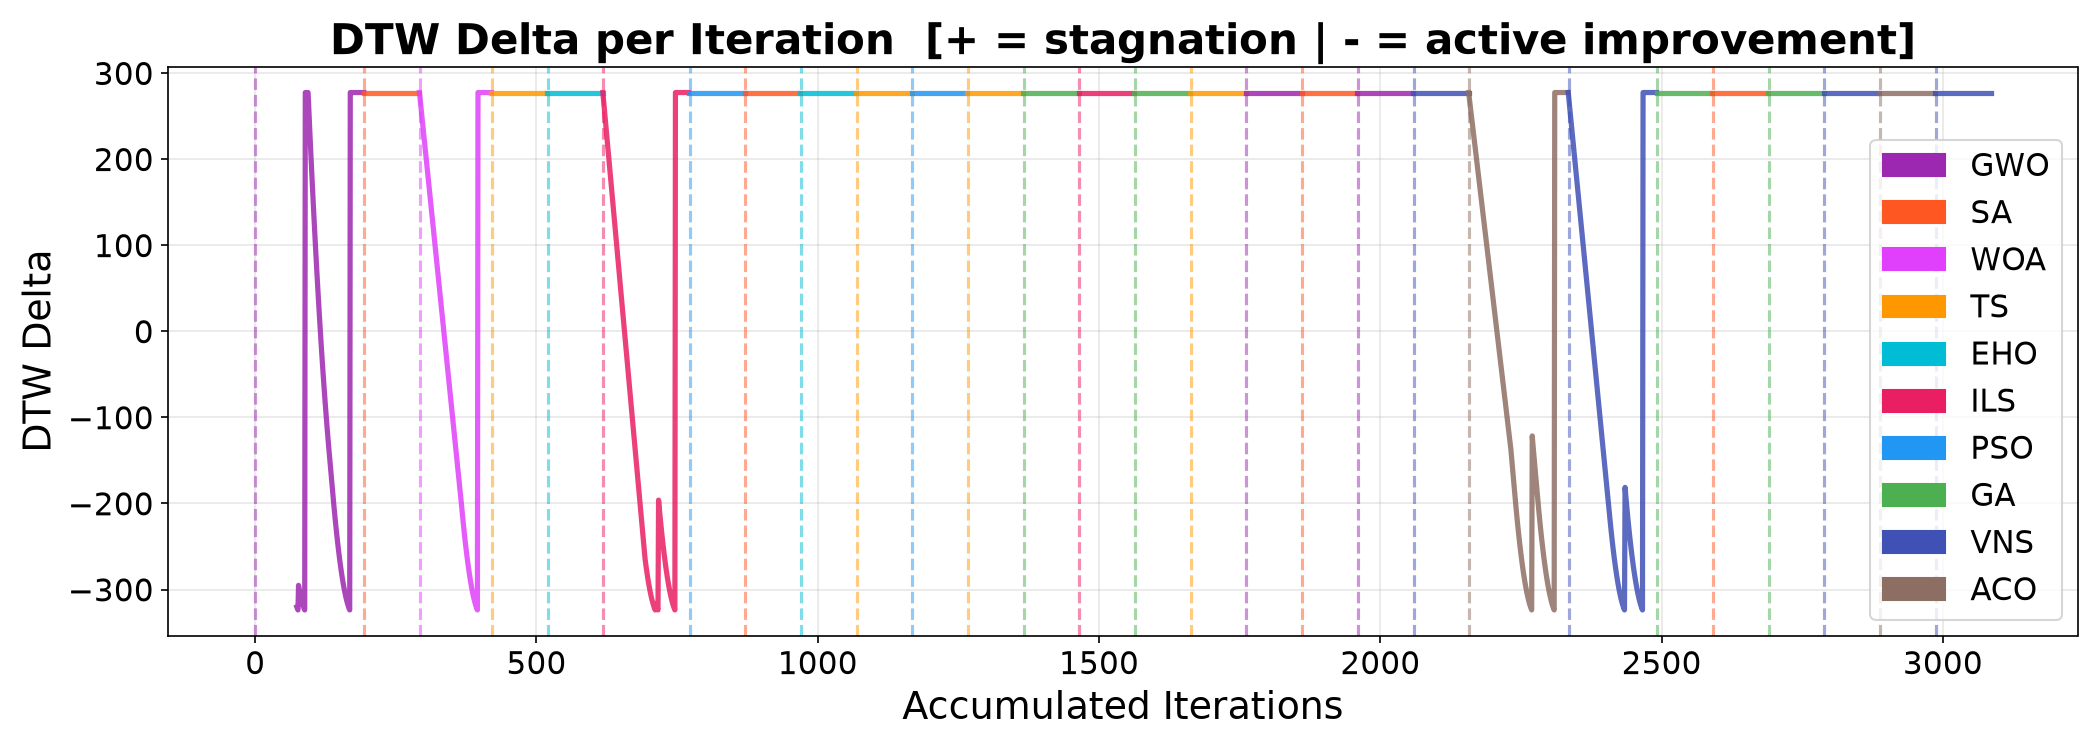
\includegraphics[width=0.32\textwidth]{imagenes_paper/mkp_dtw_3k_mknapcb4_delta.png}}
\caption{Diagnostic suite for instance \textbf{mknapcb4} ($n=100$, $m=10$) under the DTW framework with $T_{\max}=3{,}000$: (a)~final-fitness distribution over $N=31$ runs; (b)~convergence trajectory of the best run; (c)~elastic warping profile $\Delta$.}
\label{fig:mkp-best-cb4}
\end{figure}

% --- mknapcb5: DTW, 3,000 iterations ---
\begin{figure}[htbp]
\centering
\subfloat[Metaheuristic comparison.]{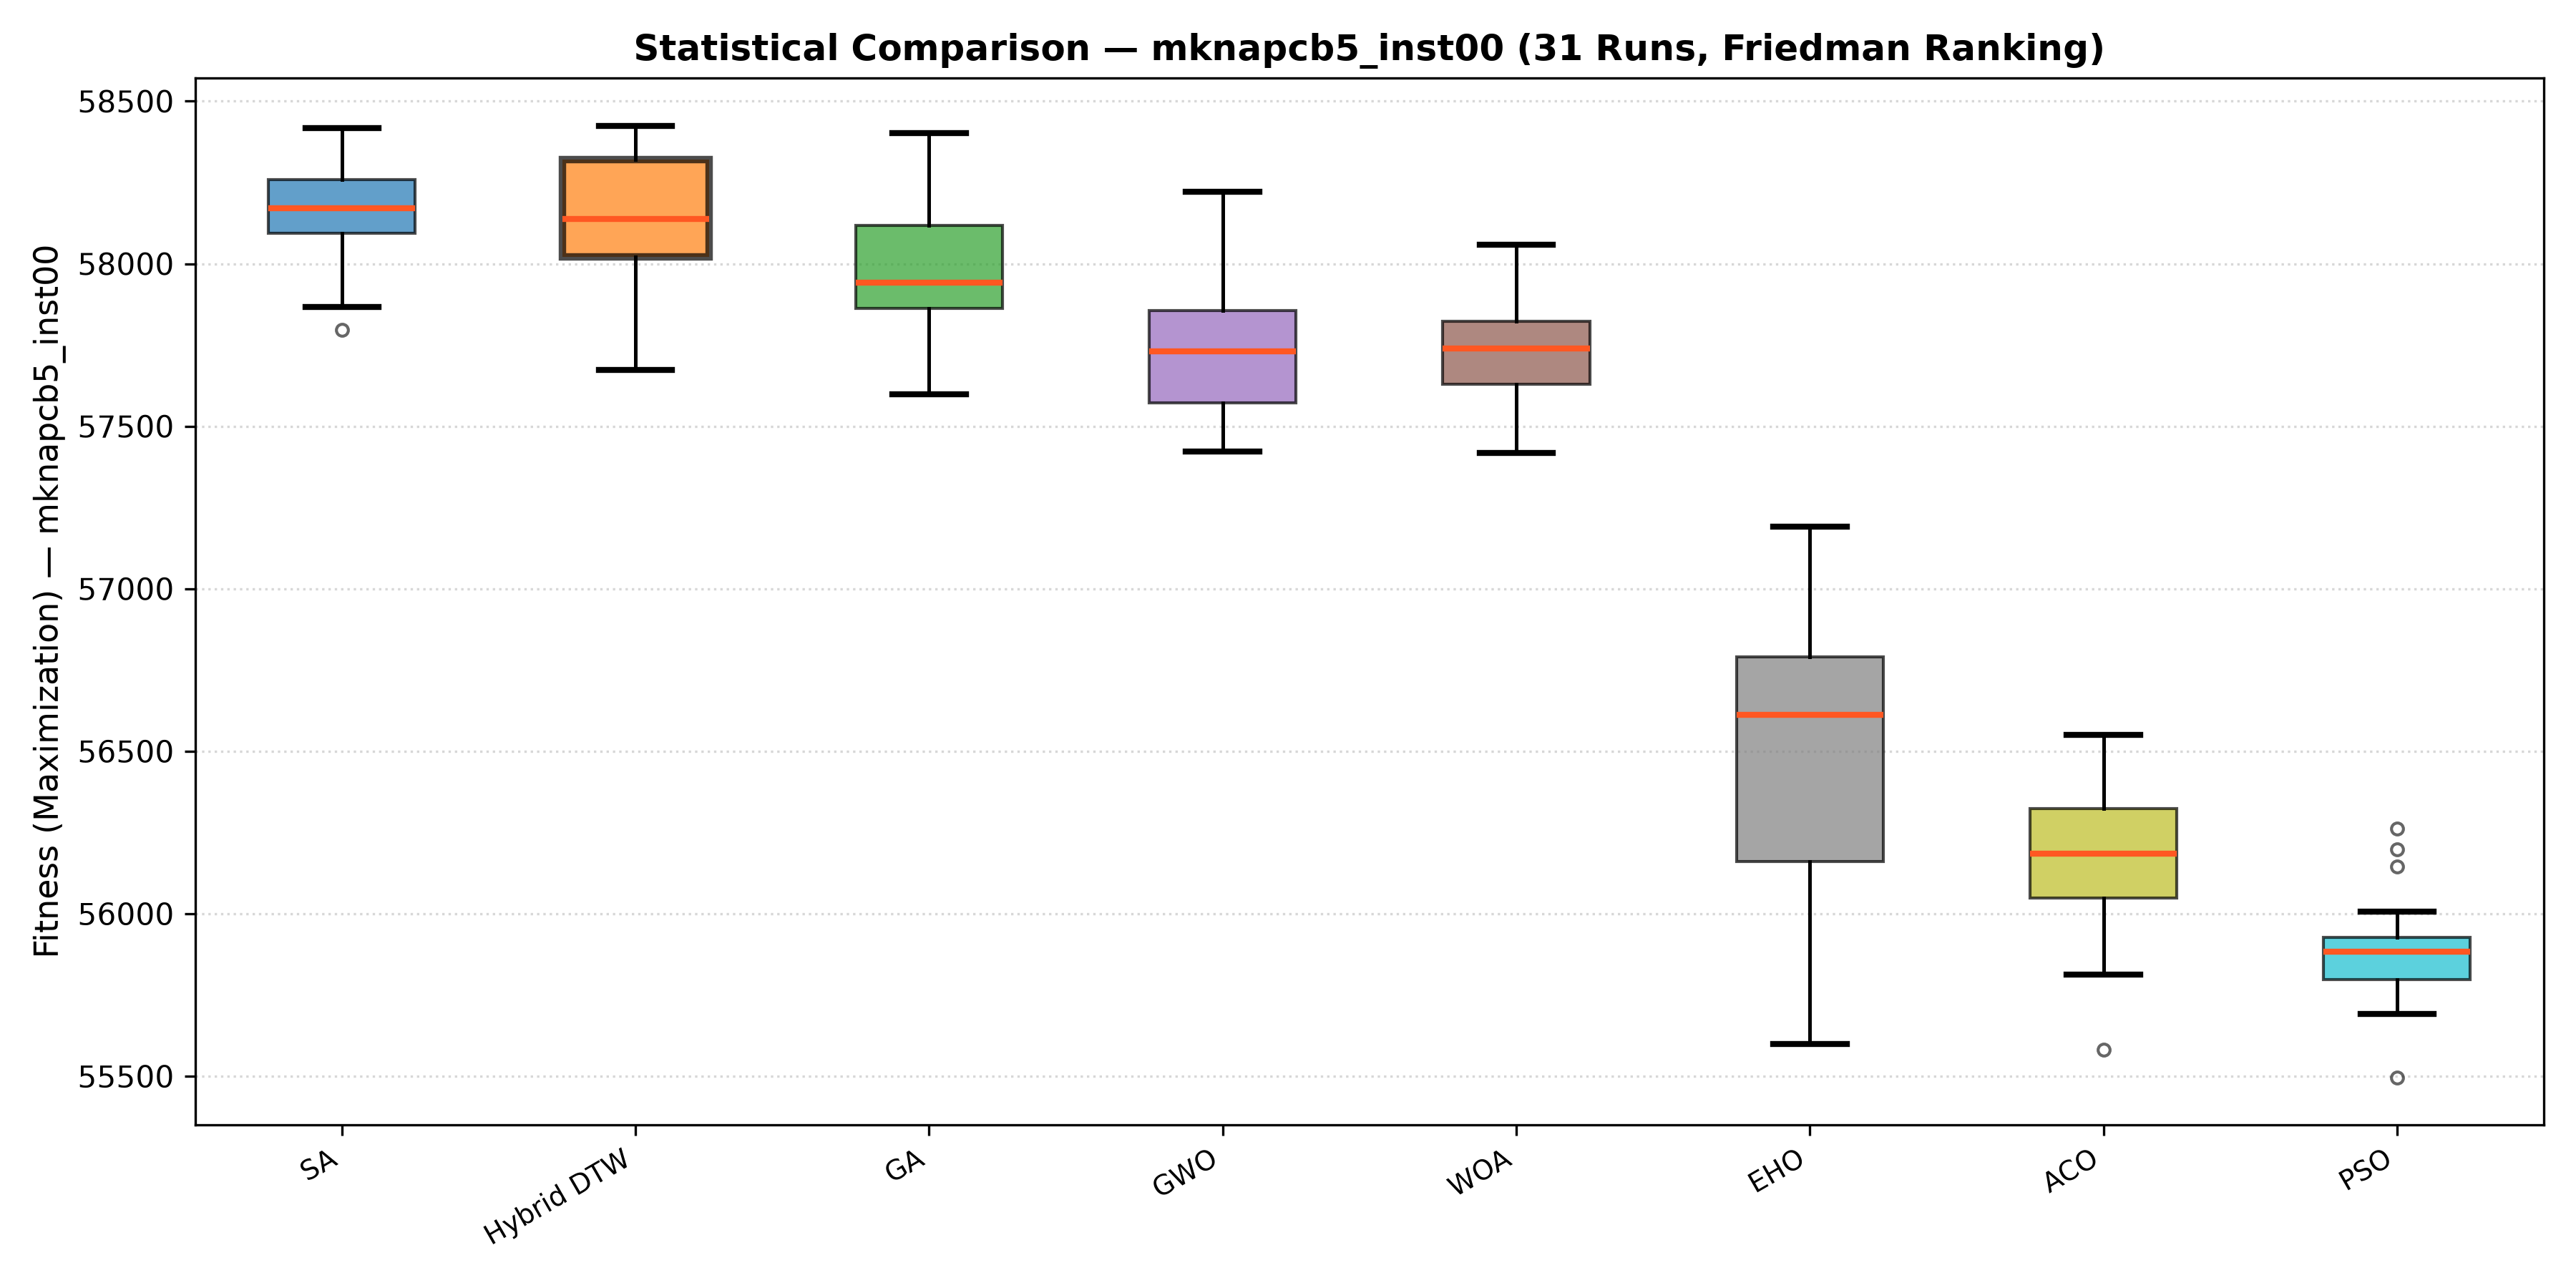
\includegraphics[width=0.32\textwidth]{imagenes_paper/mkp_dtw_3k_mknapcb5_comparativo_mh.png}}\hfill
\subfloat[Best-run convergence.]{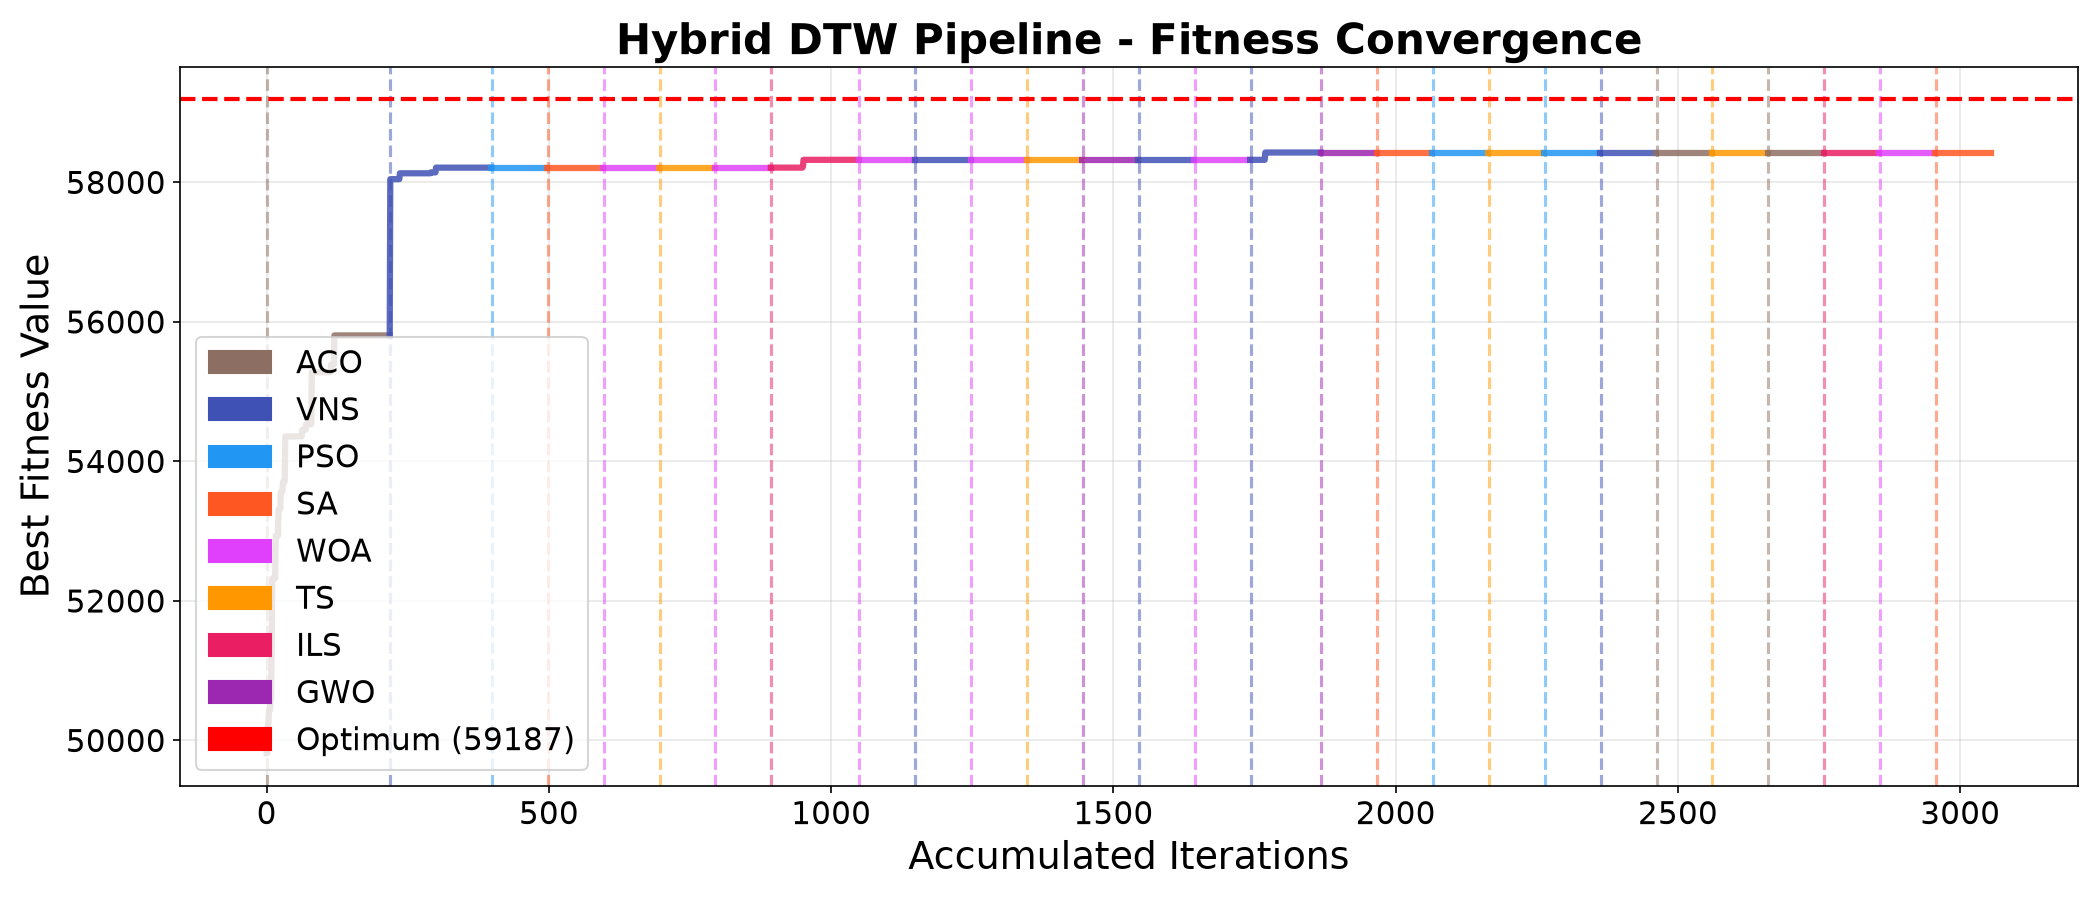
\includegraphics[width=0.32\textwidth]{imagenes_paper/mkp_dtw_3k_mknapcb5_convergencia.png}}\hfill
\subfloat[Elastic metric $\Delta=D_1-D_2$.]{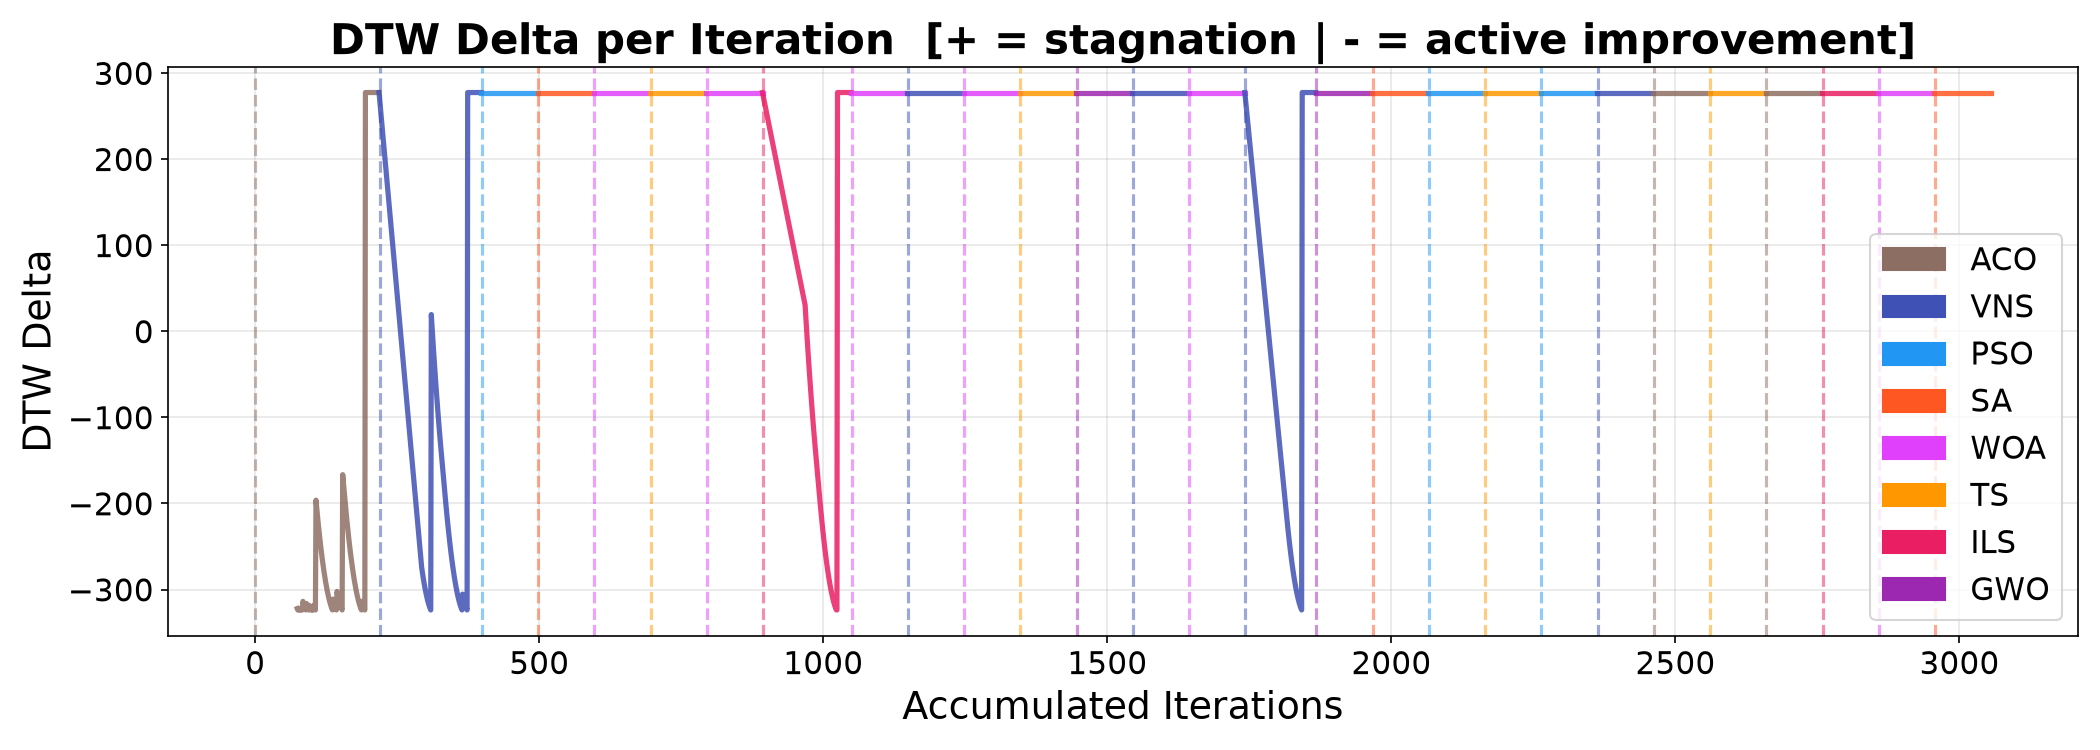
\includegraphics[width=0.32\textwidth]{imagenes_paper/mkp_dtw_3k_mknapcb5_delta.png}}
\caption{Diagnostic suite for instance \textbf{mknapcb5} ($n=250$, $m=10$) under the DTW framework with $T_{\max}=3{,}000$: (a)~final-fitness distribution over $N=31$ runs; (b)~convergence trajectory of the best run; (c)~elastic warping profile $\Delta$.}
\label{fig:mkp-best-cb5}
\end{figure}

% --- mknapcb6: DTW, 3,000 iterations ---
\begin{figure}[htbp]
\centering
\subfloat[Metaheuristic comparison.]{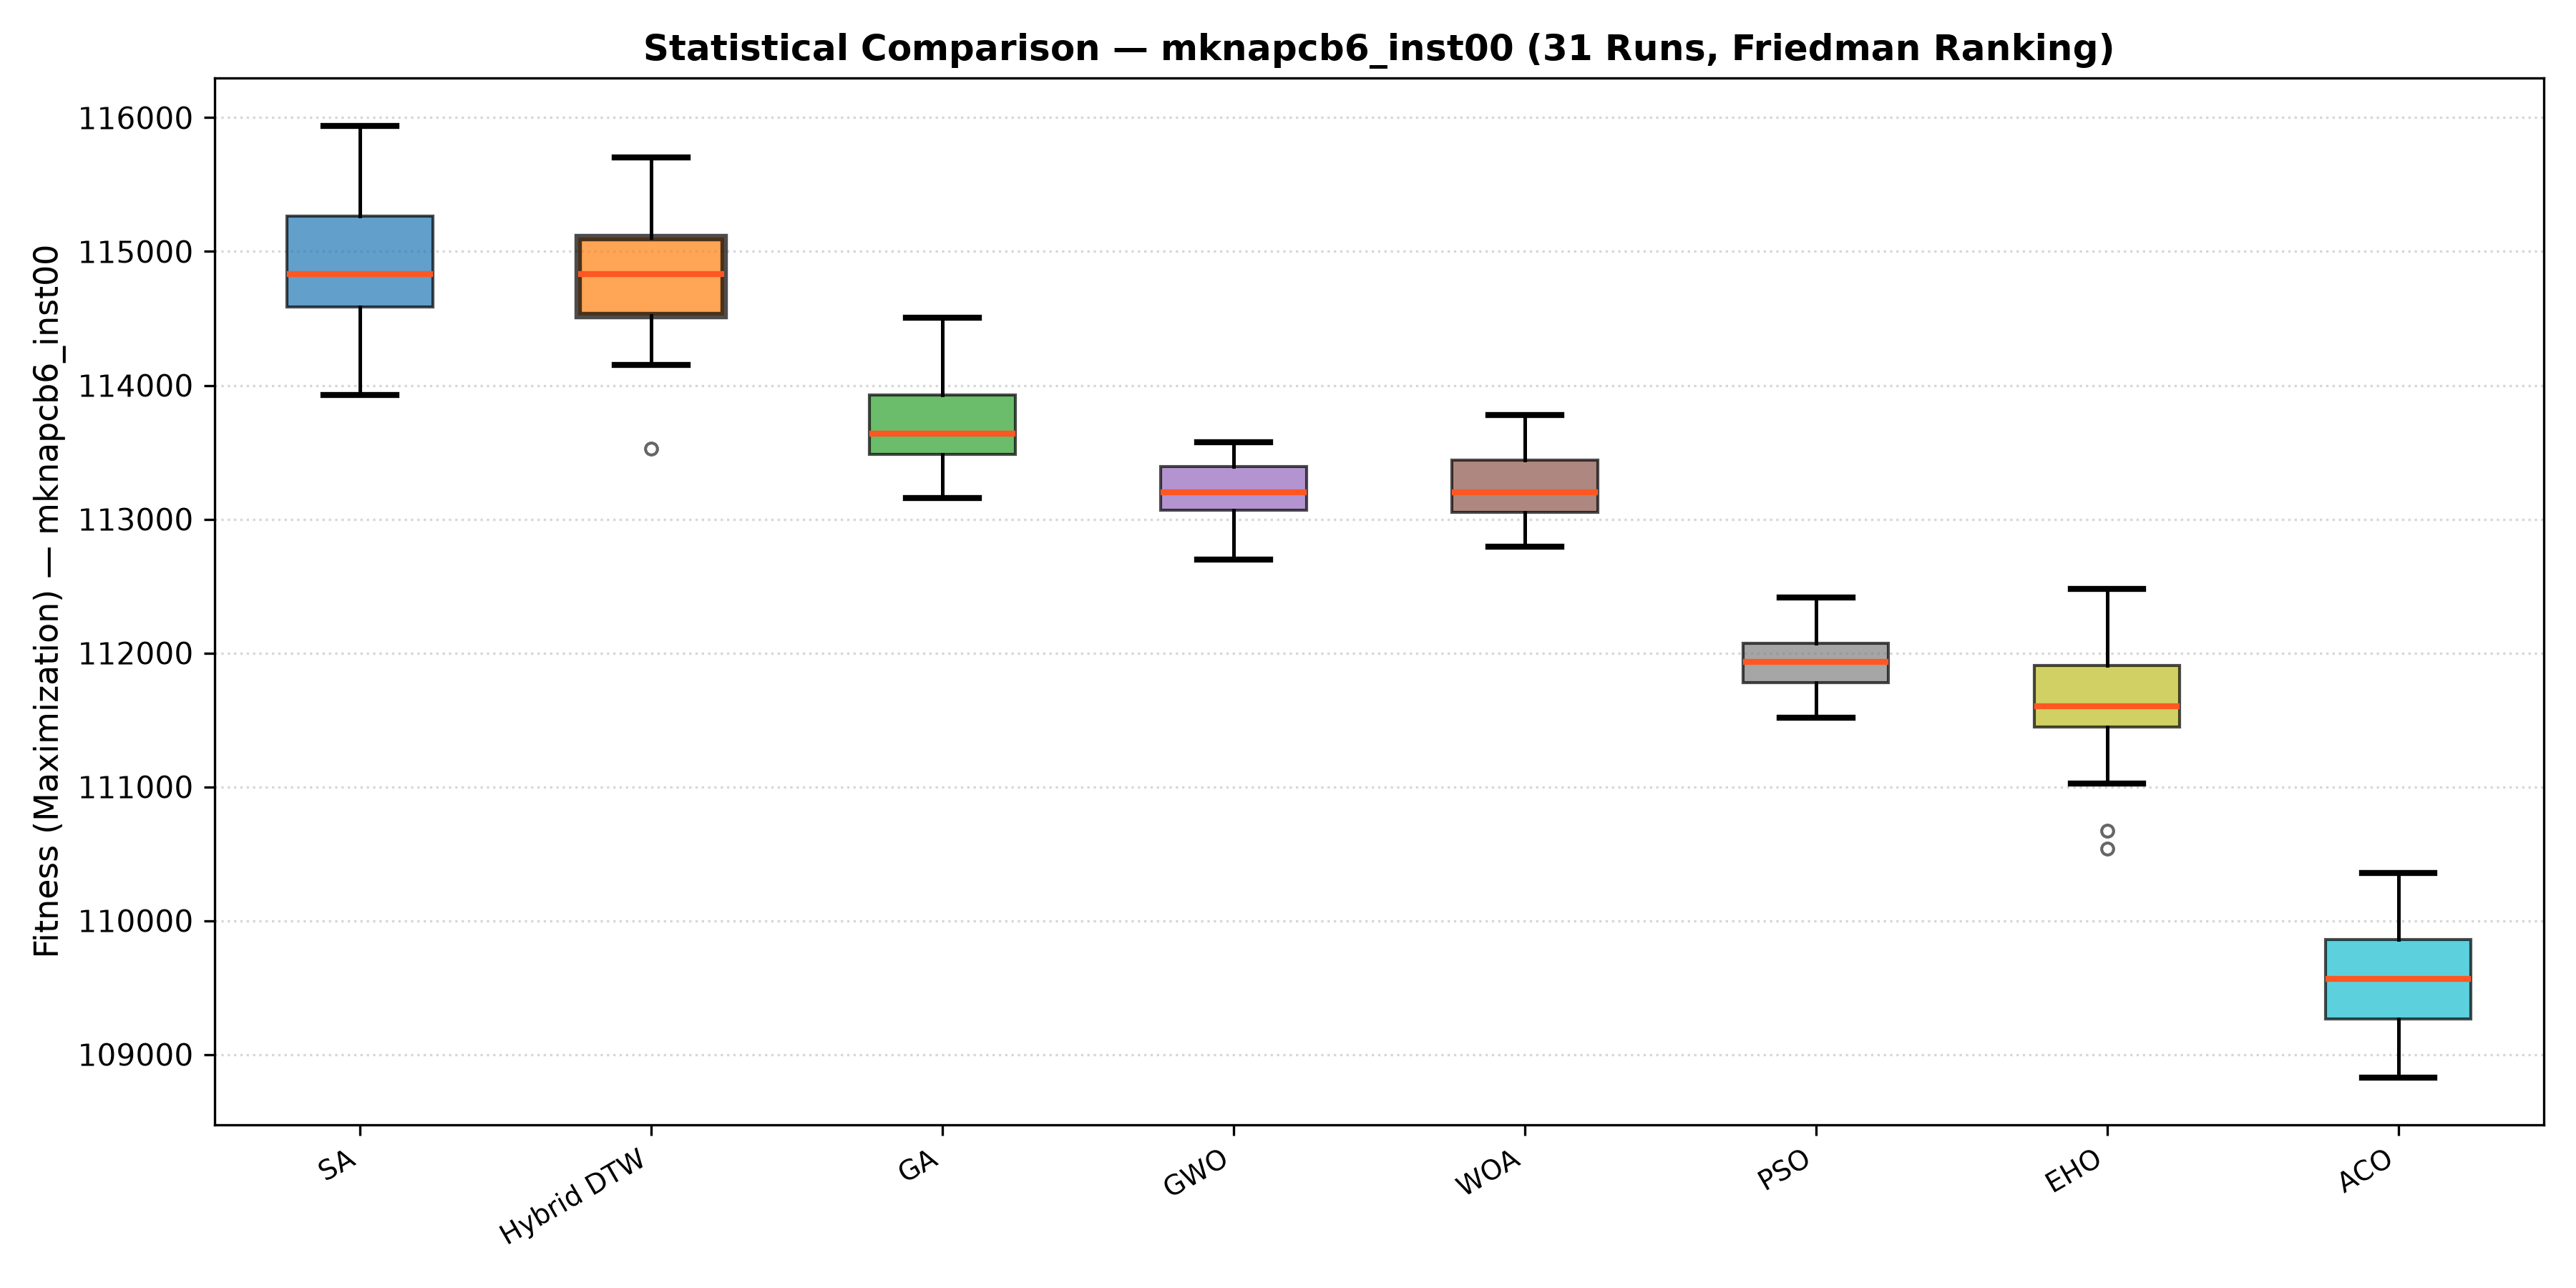
\includegraphics[width=0.32\textwidth]{imagenes_paper/mkp_dtw_3k_mknapcb6_comparativo_mh.png}}\hfill
\subfloat[Best-run convergence.]{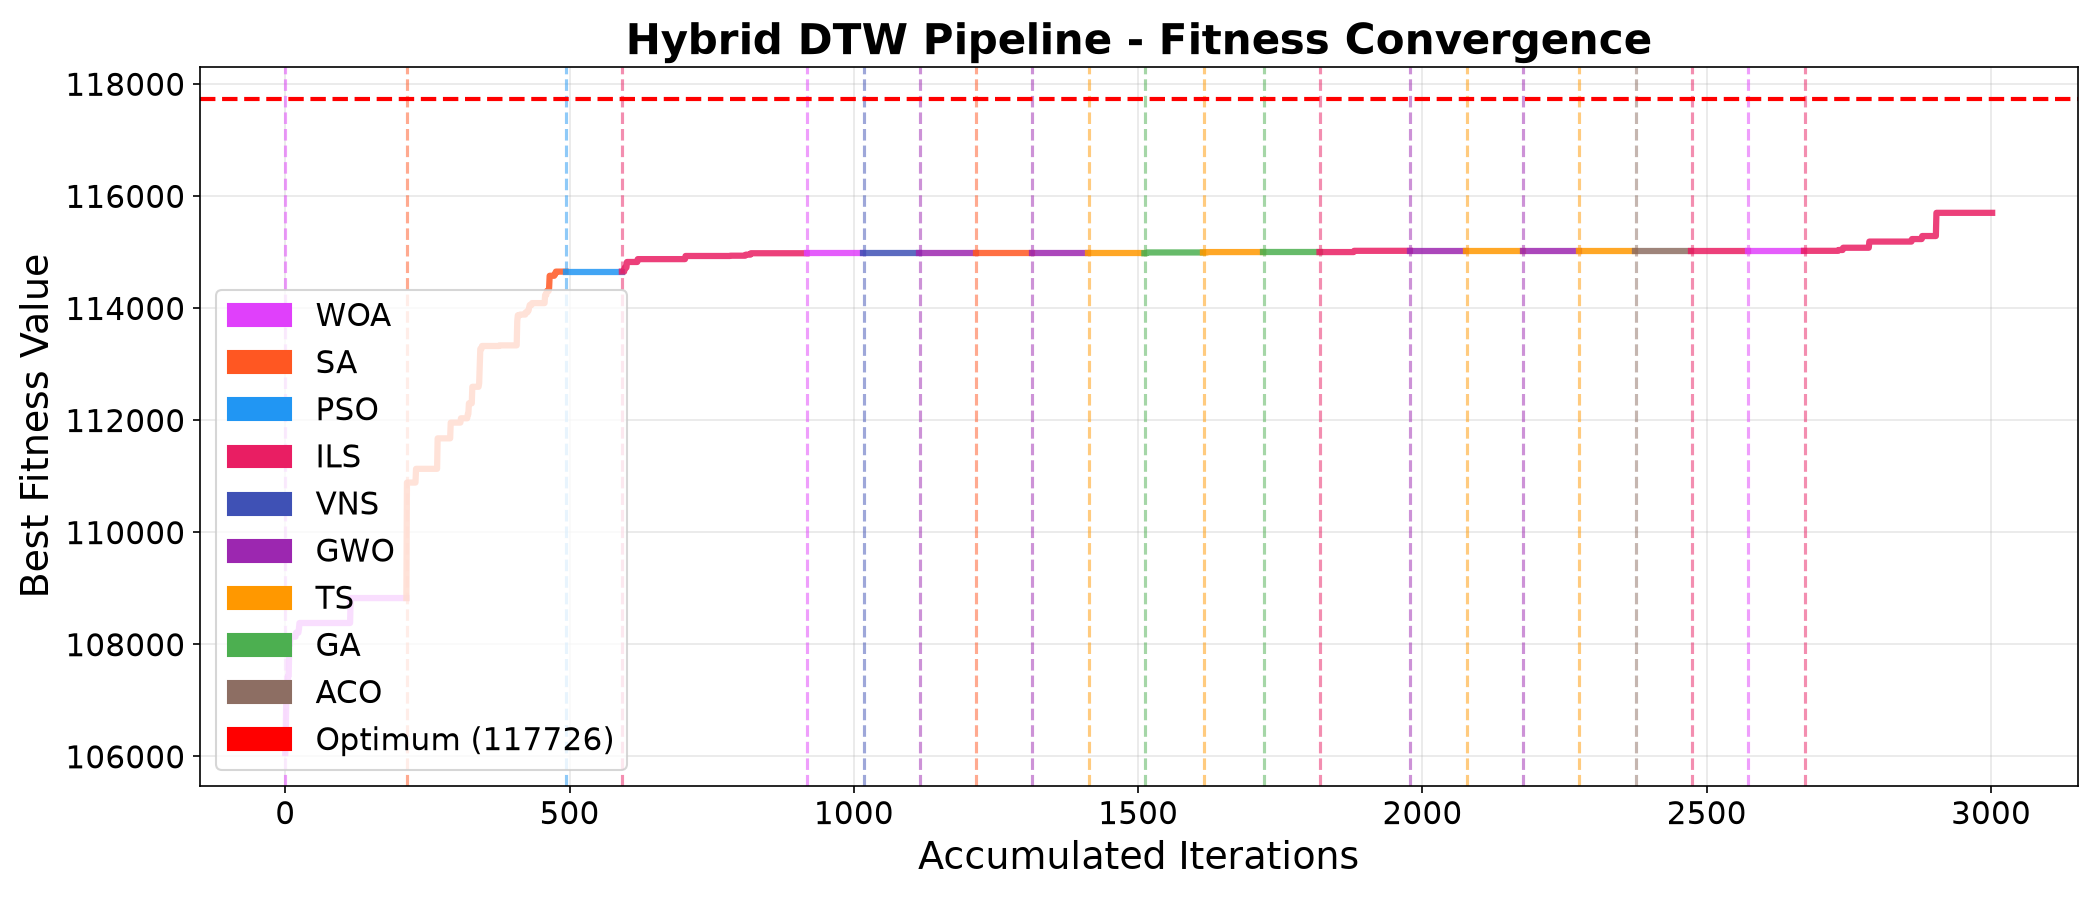
\includegraphics[width=0.32\textwidth]{imagenes_paper/mkp_dtw_3k_mknapcb6_convergencia.png}}\hfill
\subfloat[Elastic metric $\Delta=D_1-D_2$.]{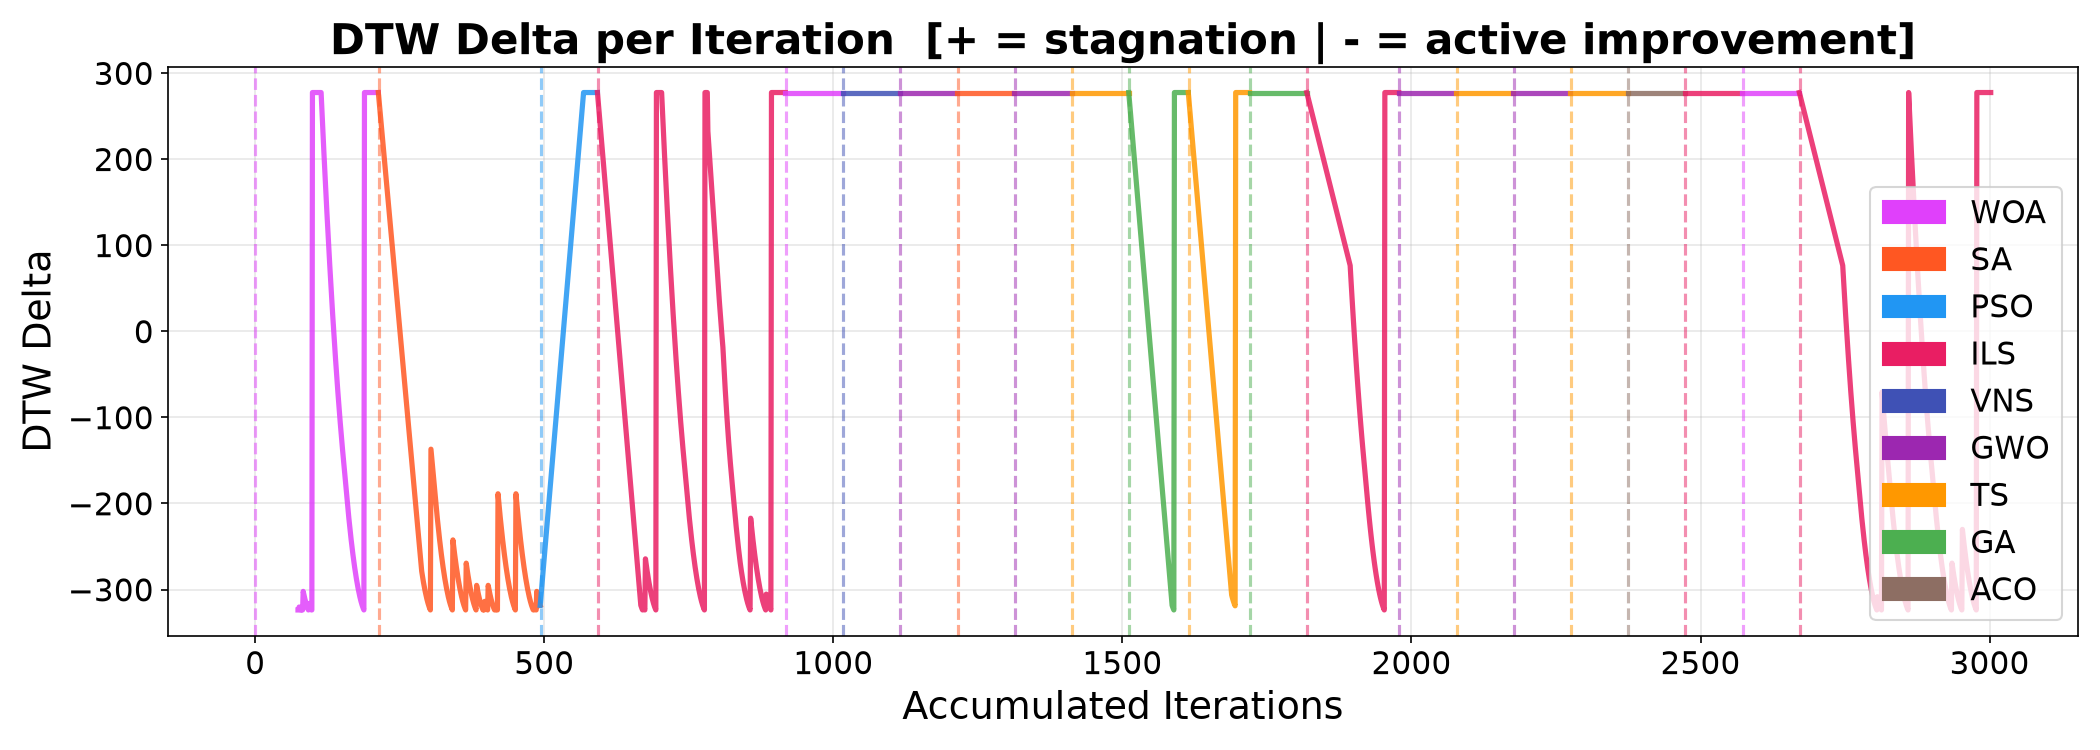
\includegraphics[width=0.32\textwidth]{imagenes_paper/mkp_dtw_3k_mknapcb6_delta.png}}
\caption{Diagnostic suite for instance \textbf{mknapcb6} ($n=500$, $m=10$) under the DTW framework with $T_{\max}=3{,}000$: (a)~final-fitness distribution over $N=31$ runs; (b)~convergence trajectory of the best run; (c)~elastic warping profile $\Delta$.}
\label{fig:mkp-best-cb6}
\end{figure}

% --- mknapcb7: DTW, 3,000 iterations ---
\begin{figure}[htbp]
\centering
\subfloat[Metaheuristic comparison.]{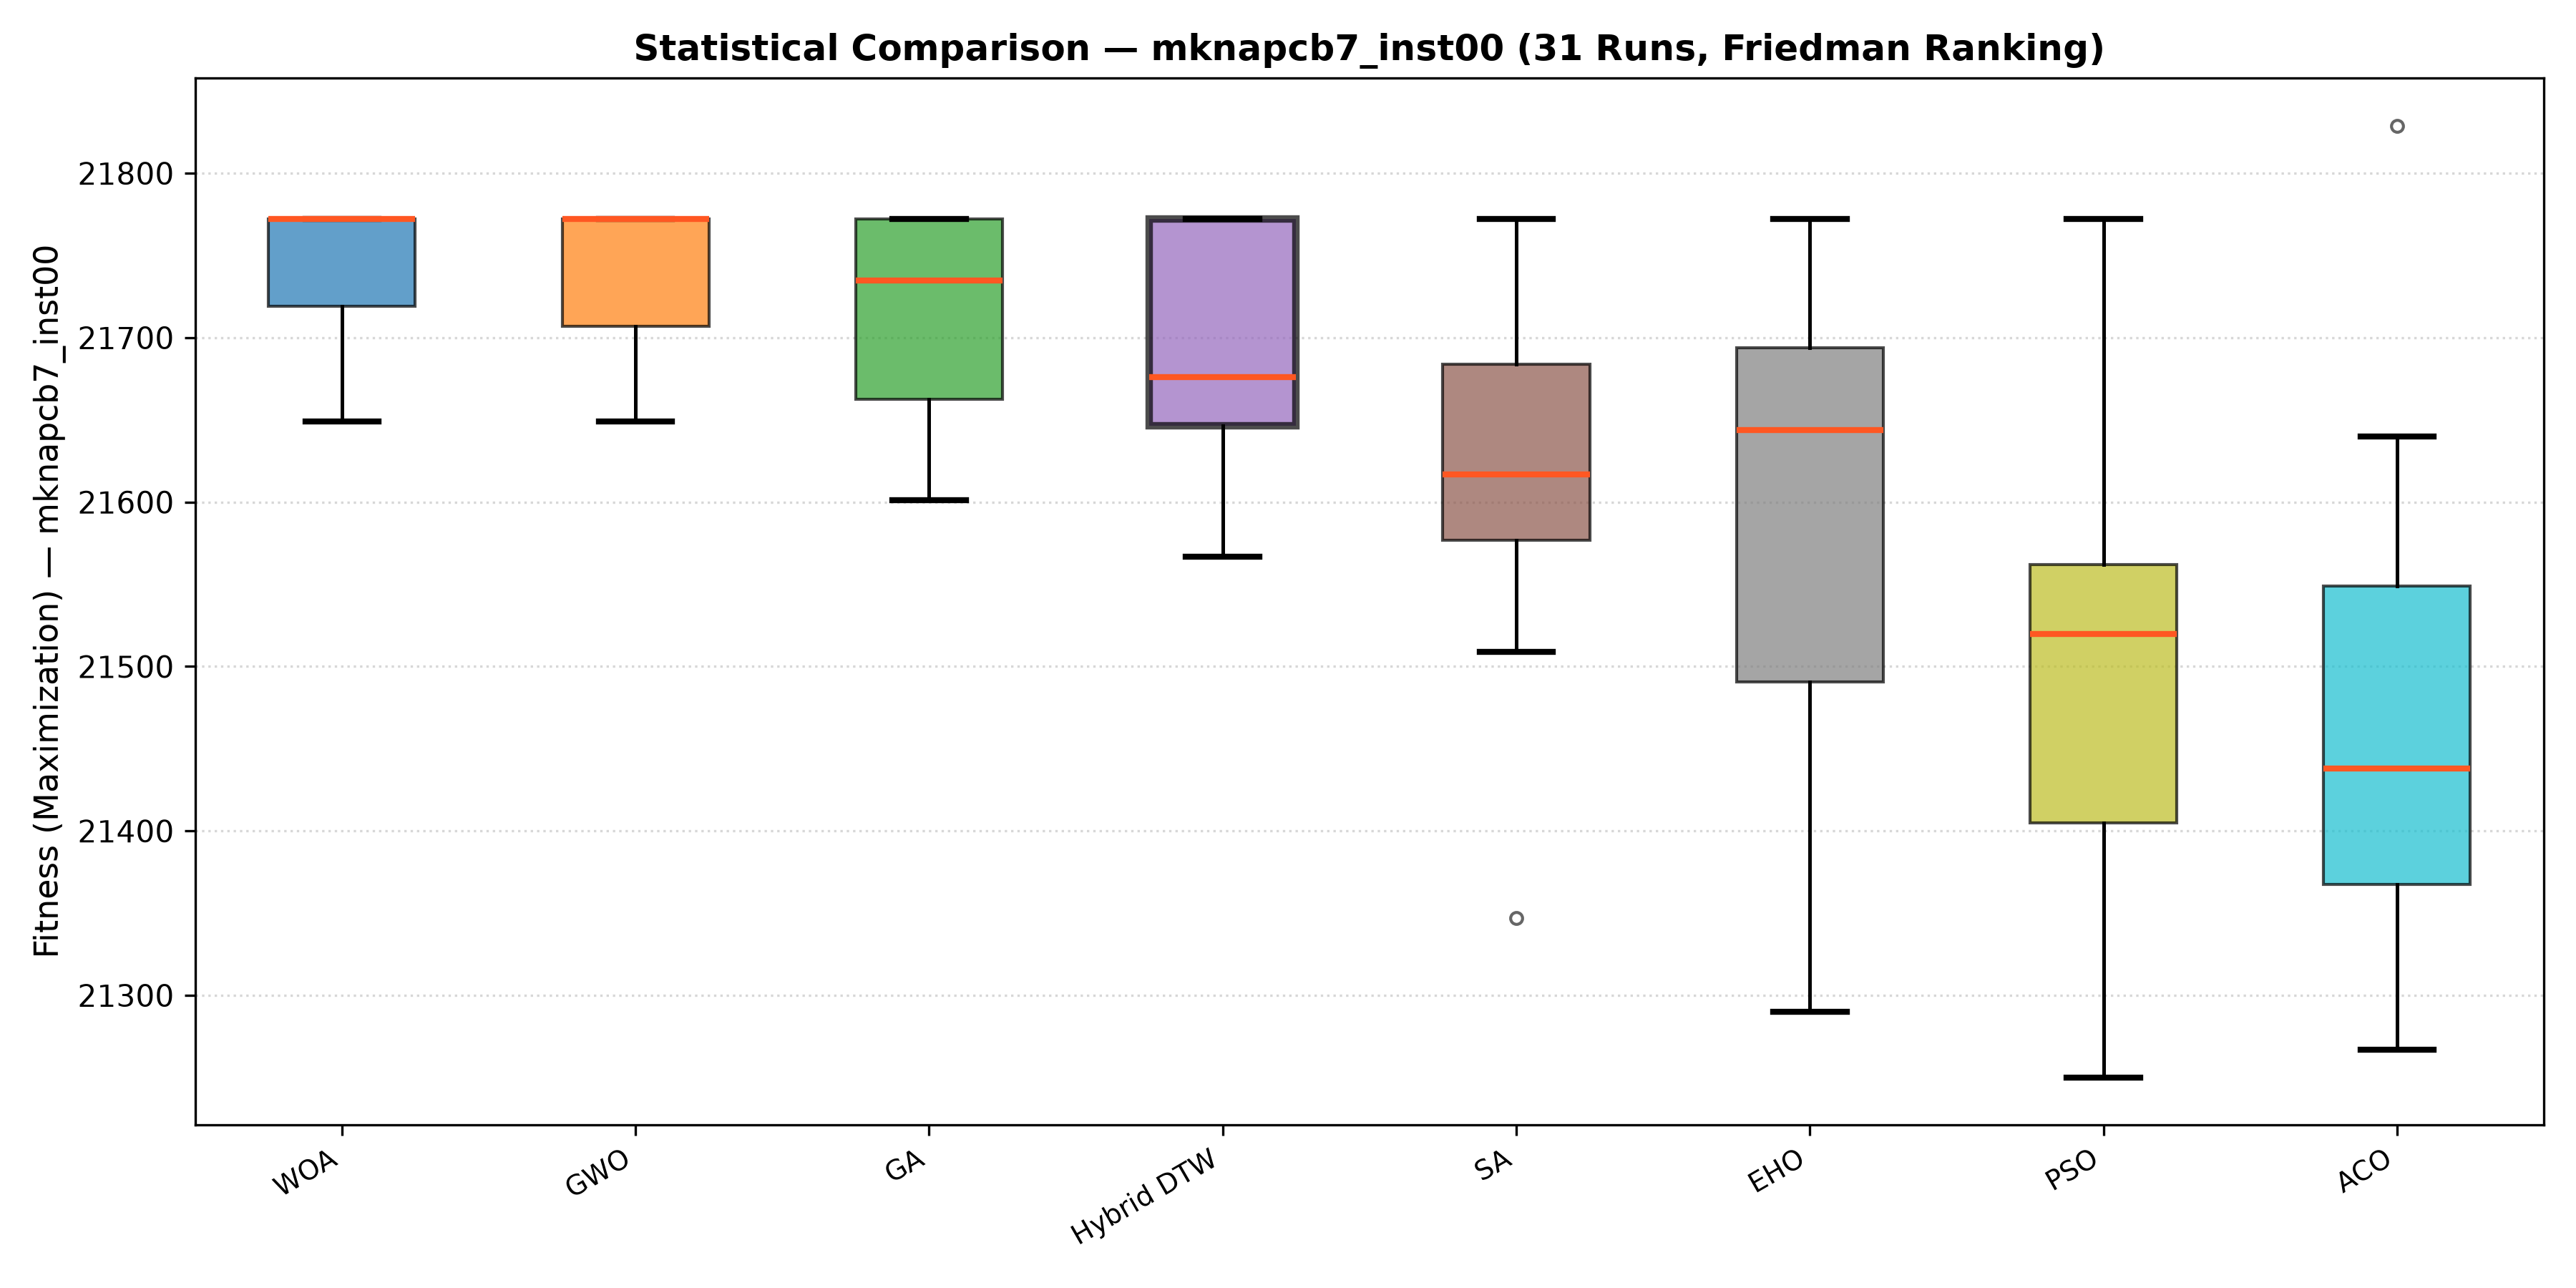
\includegraphics[width=0.32\textwidth]{imagenes_paper/mkp_dtw_3k_mknapcb7_comparativo_mh.png}}\hfill
\subfloat[Best-run convergence.]{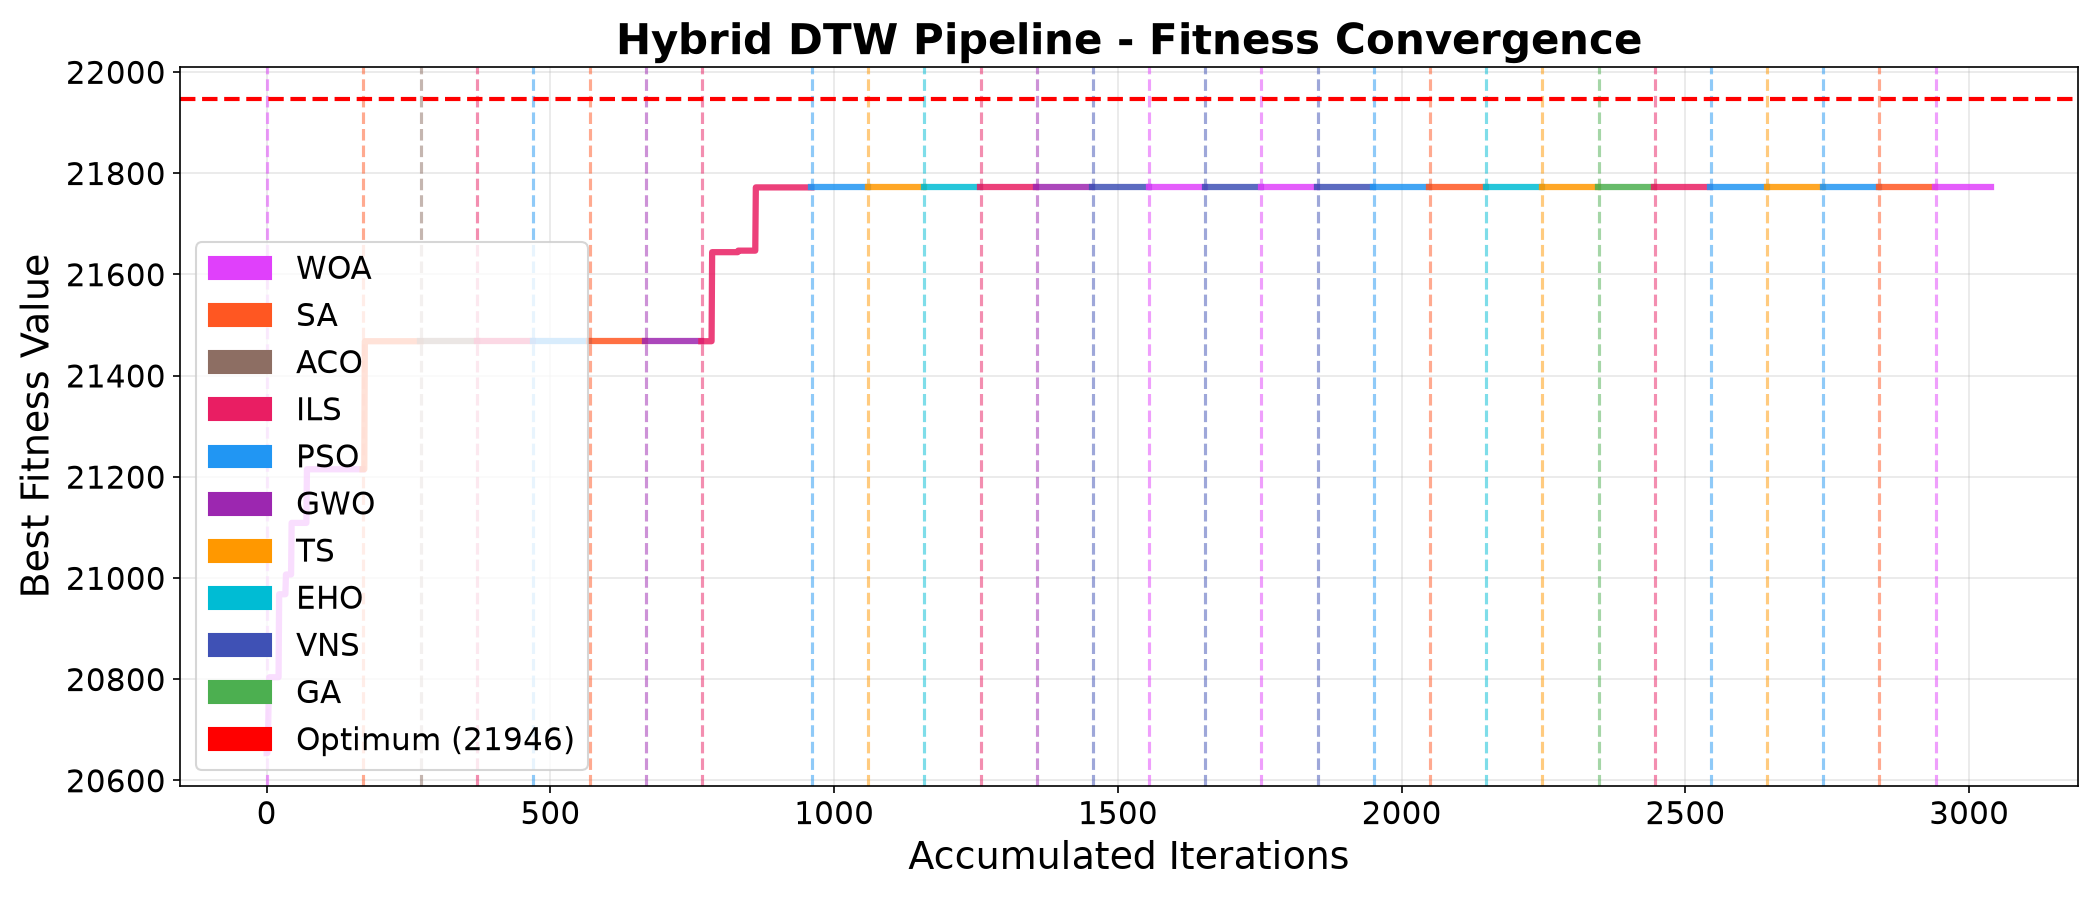
\includegraphics[width=0.32\textwidth]{imagenes_paper/mkp_dtw_3k_mknapcb7_convergencia.png}}\hfill
\subfloat[Elastic metric $\Delta=D_1-D_2$.]{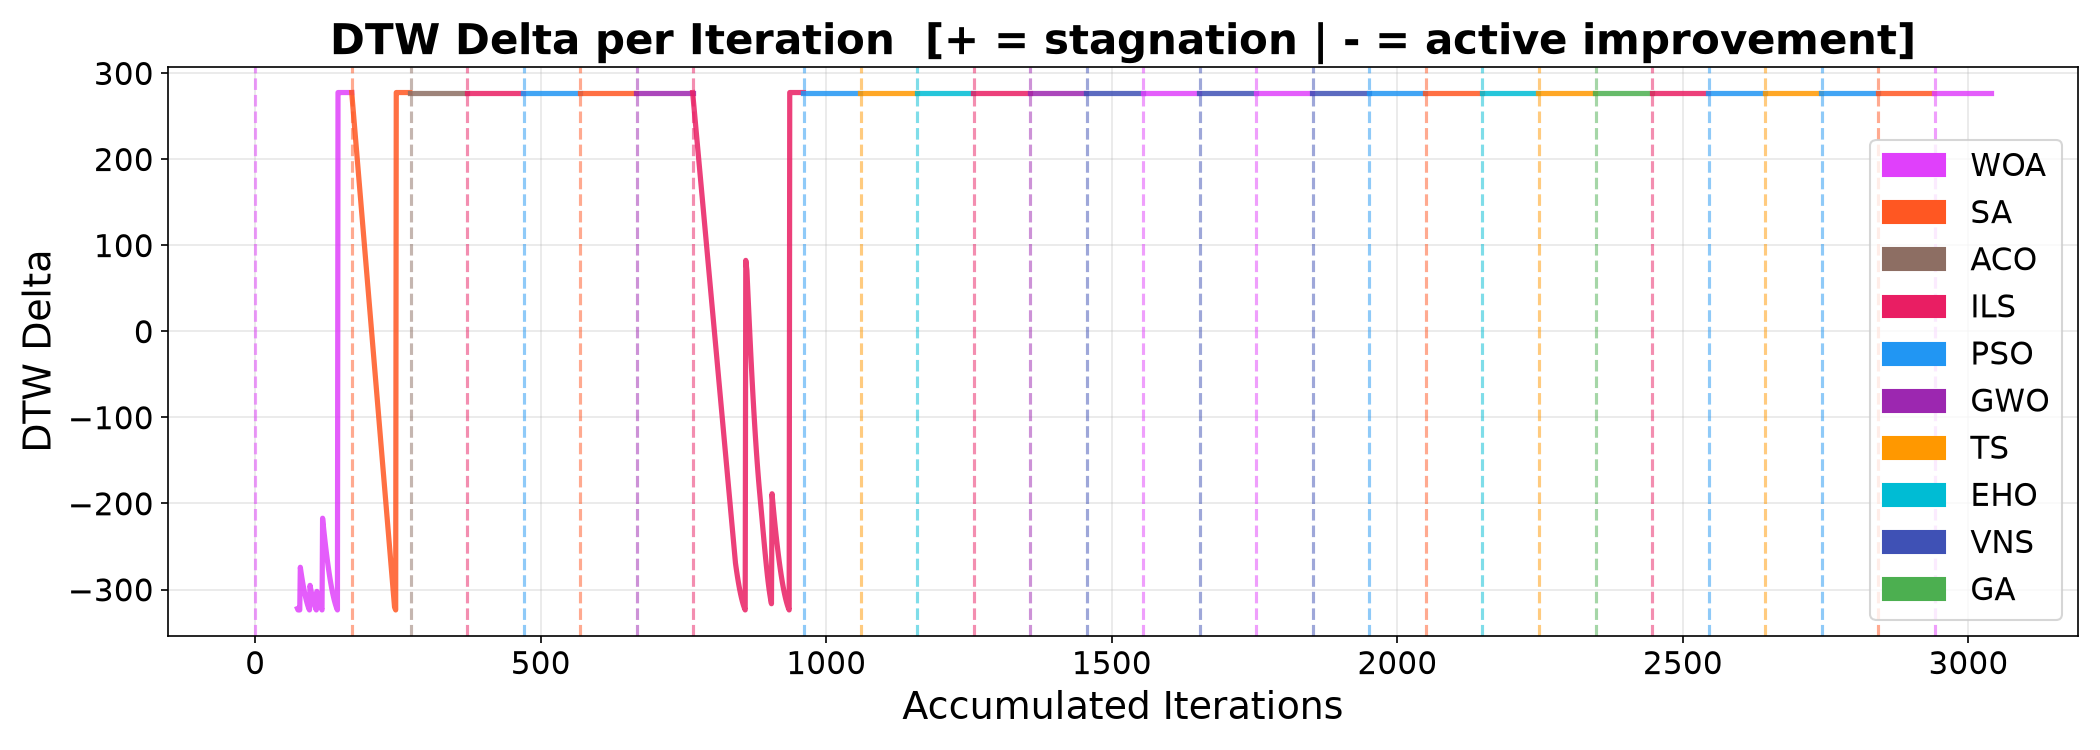
\includegraphics[width=0.32\textwidth]{imagenes_paper/mkp_dtw_3k_mknapcb7_delta.png}}
\caption{Diagnostic suite for instance \textbf{mknapcb7} ($n=100$, $m=30$) under the DTW framework with $T_{\max}=3{,}000$: (a)~final-fitness distribution over $N=31$ runs; (b)~convergence trajectory of the best run; (c)~elastic warping profile $\Delta$.}
\label{fig:mkp-best-cb7}
\end{figure}

% --- mknapcb8: DTW, 3,000 iterations ---
\begin{figure}[htbp]
\centering
\subfloat[Metaheuristic comparison.]{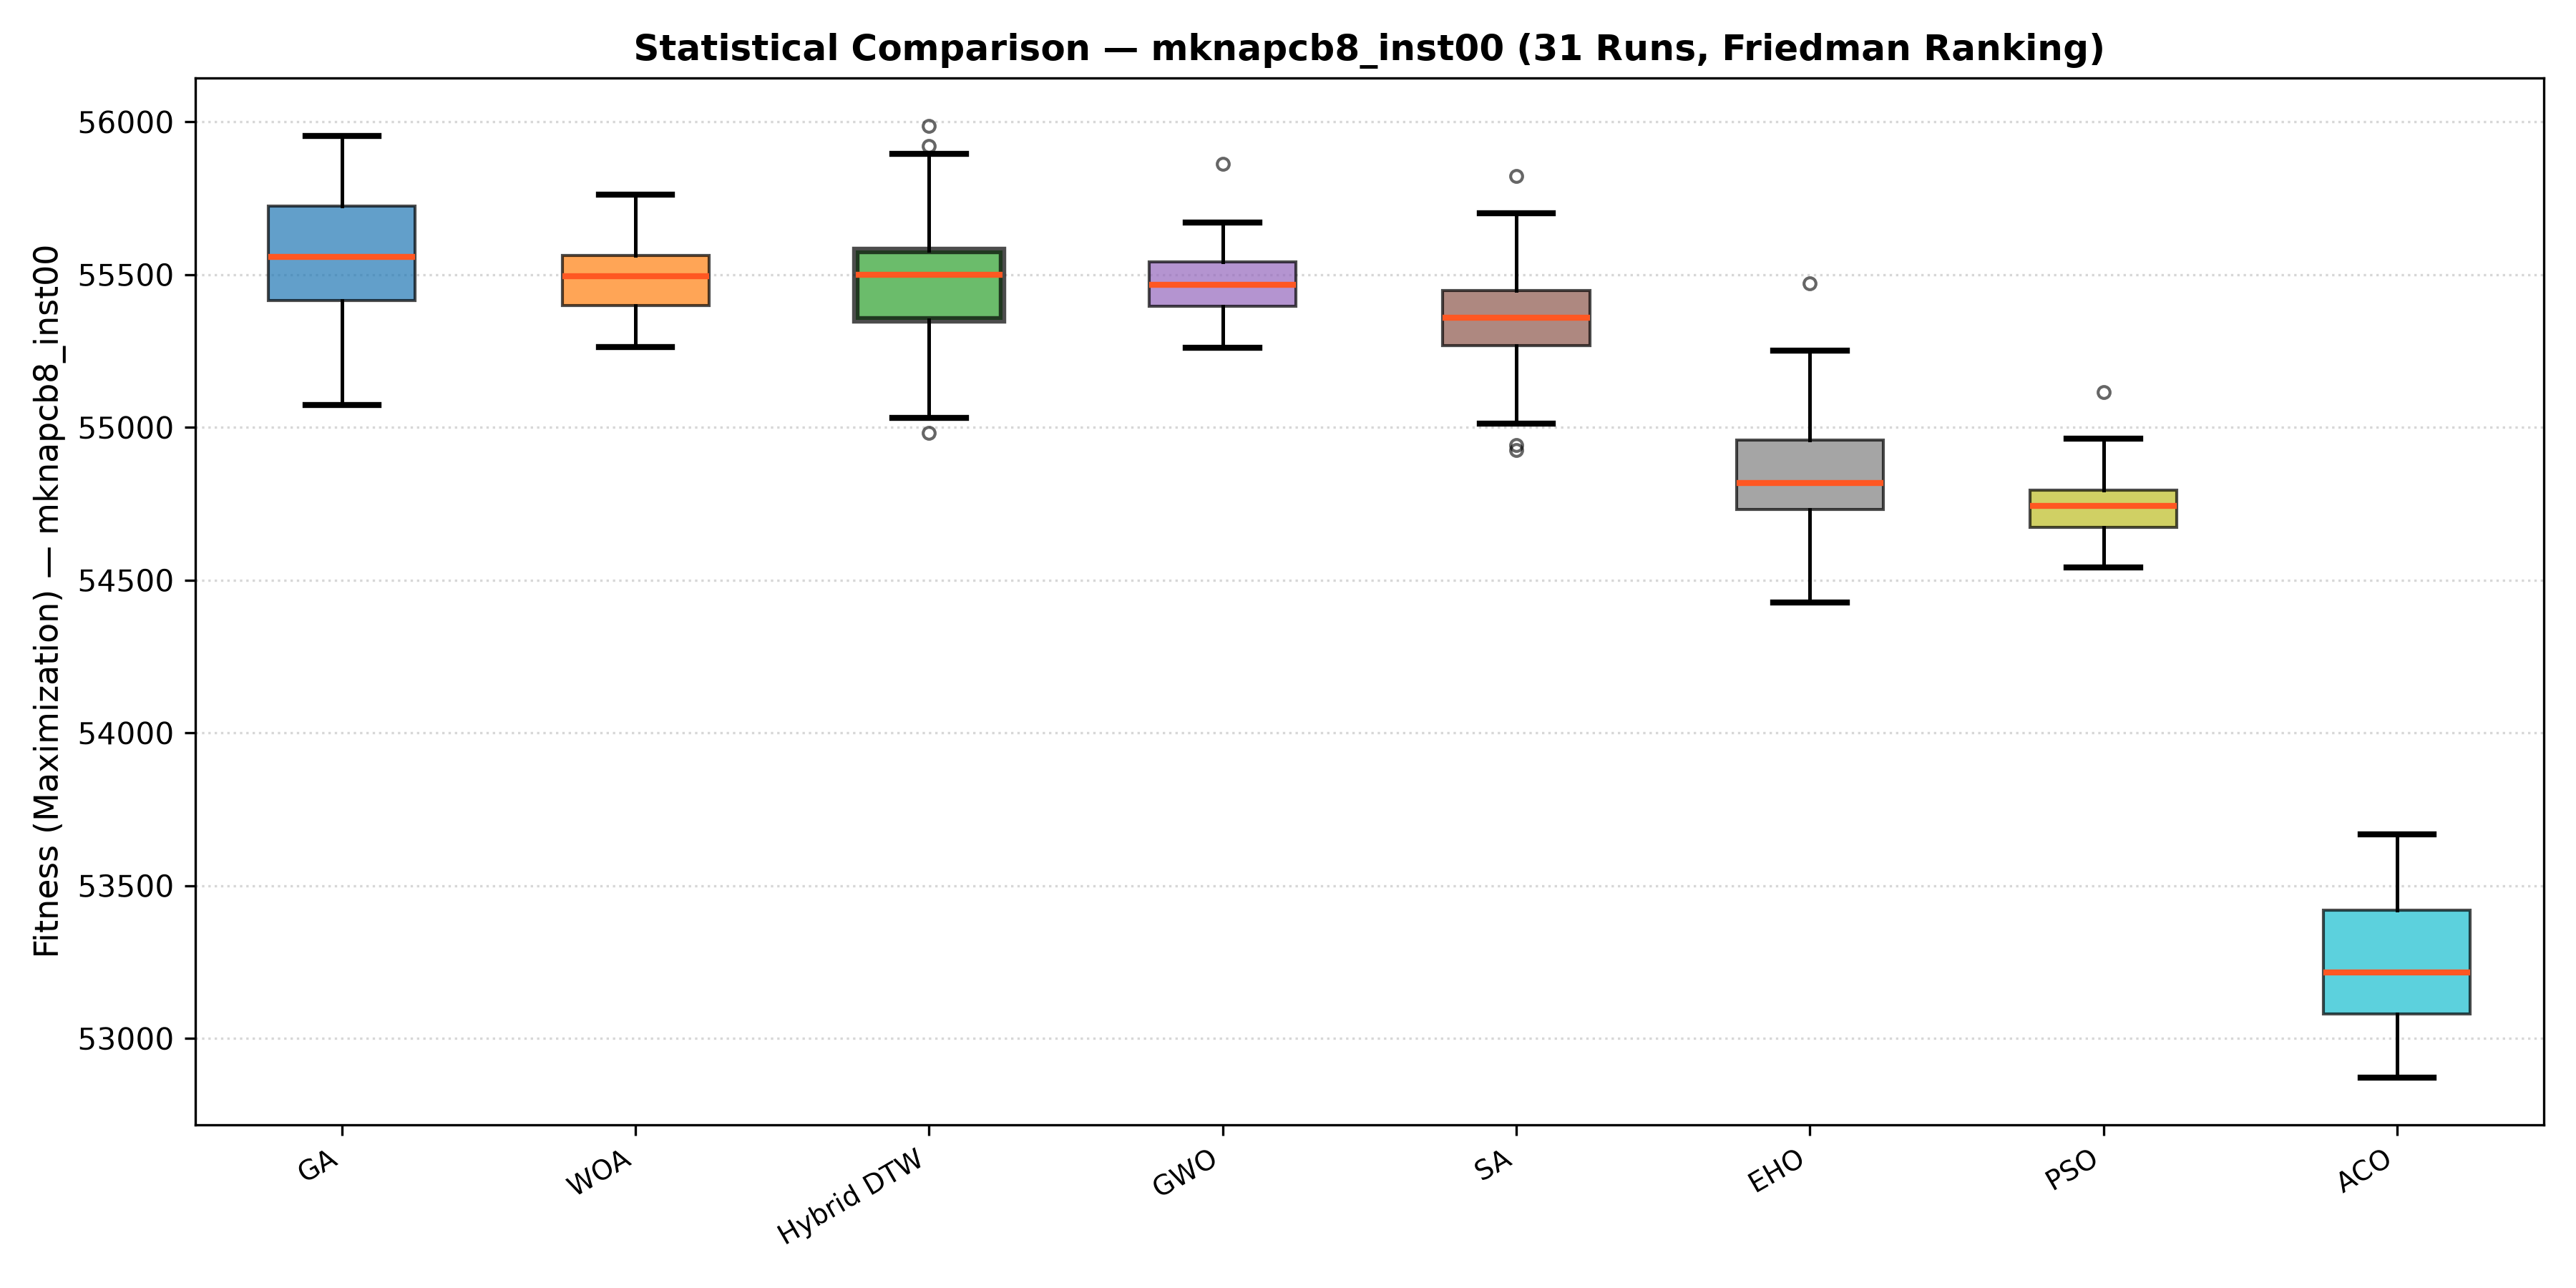
\includegraphics[width=0.32\textwidth]{imagenes_paper/mkp_dtw_3k_mknapcb8_comparativo_mh.png}}\hfill
\subfloat[Best-run convergence.]{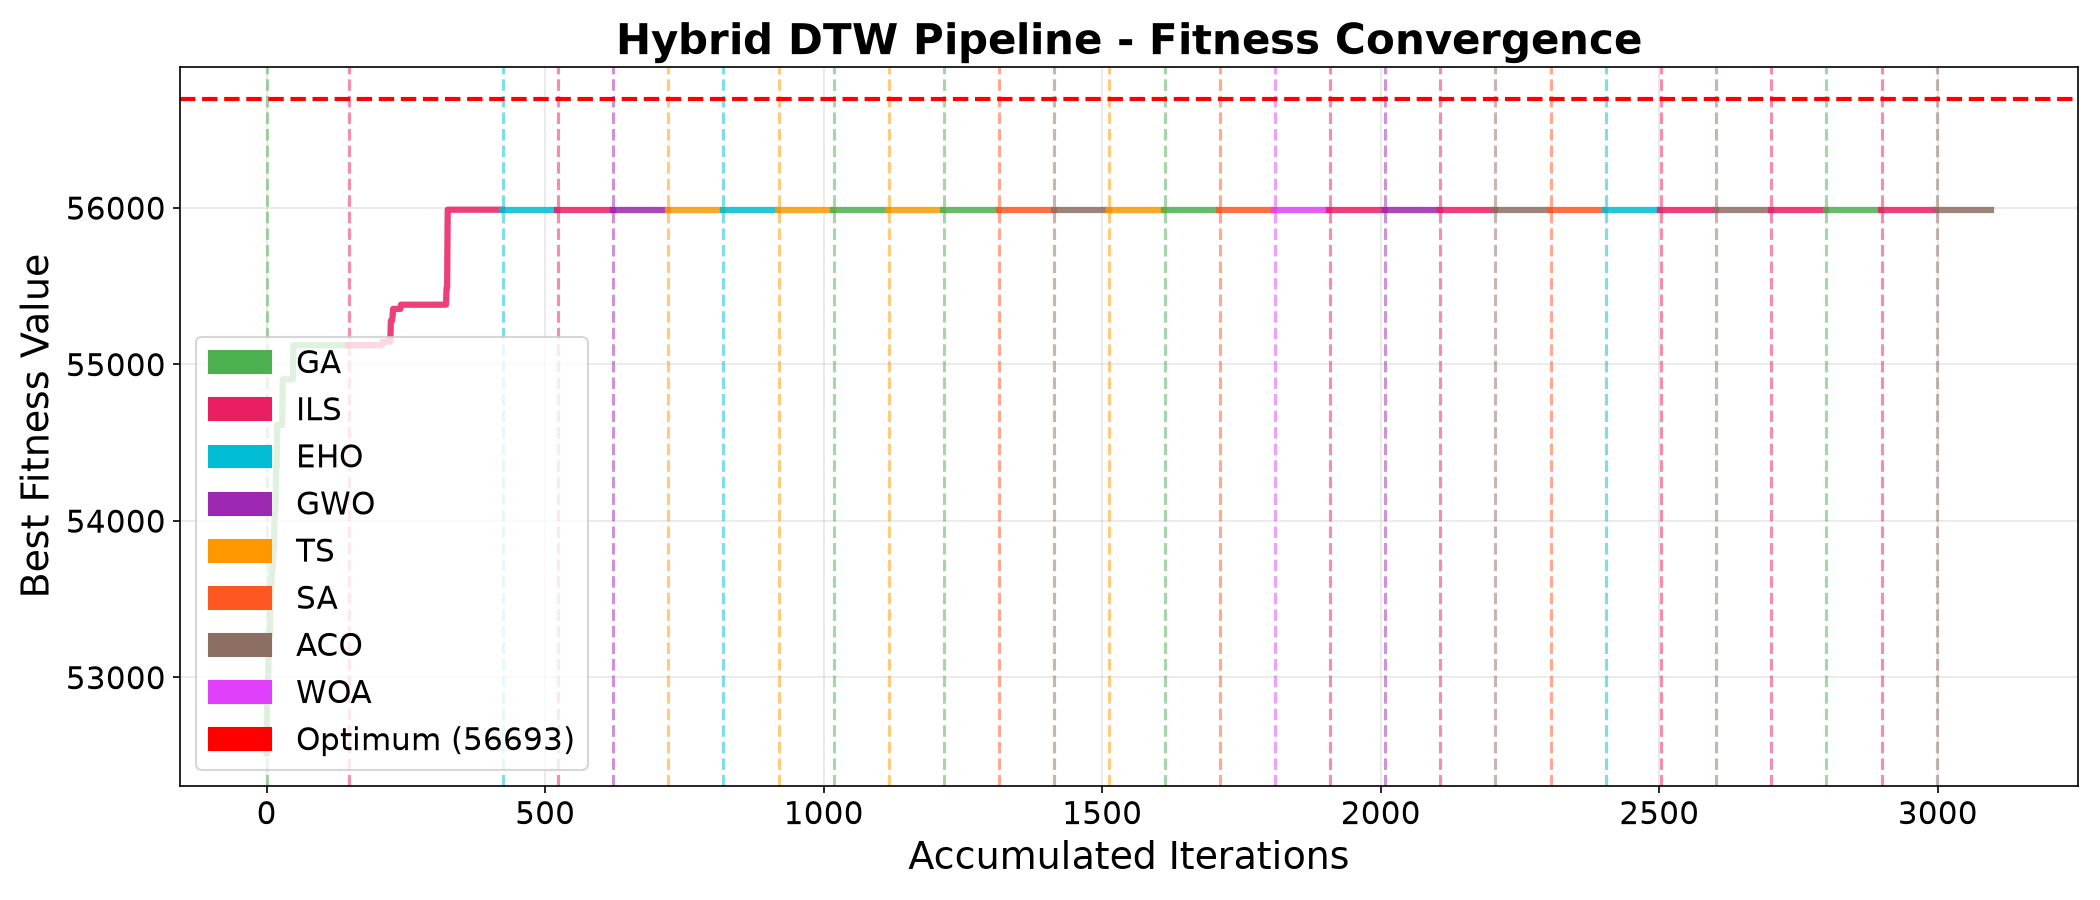
\includegraphics[width=0.32\textwidth]{imagenes_paper/mkp_dtw_3k_mknapcb8_convergencia.png}}\hfill
\subfloat[Elastic metric $\Delta=D_1-D_2$.]{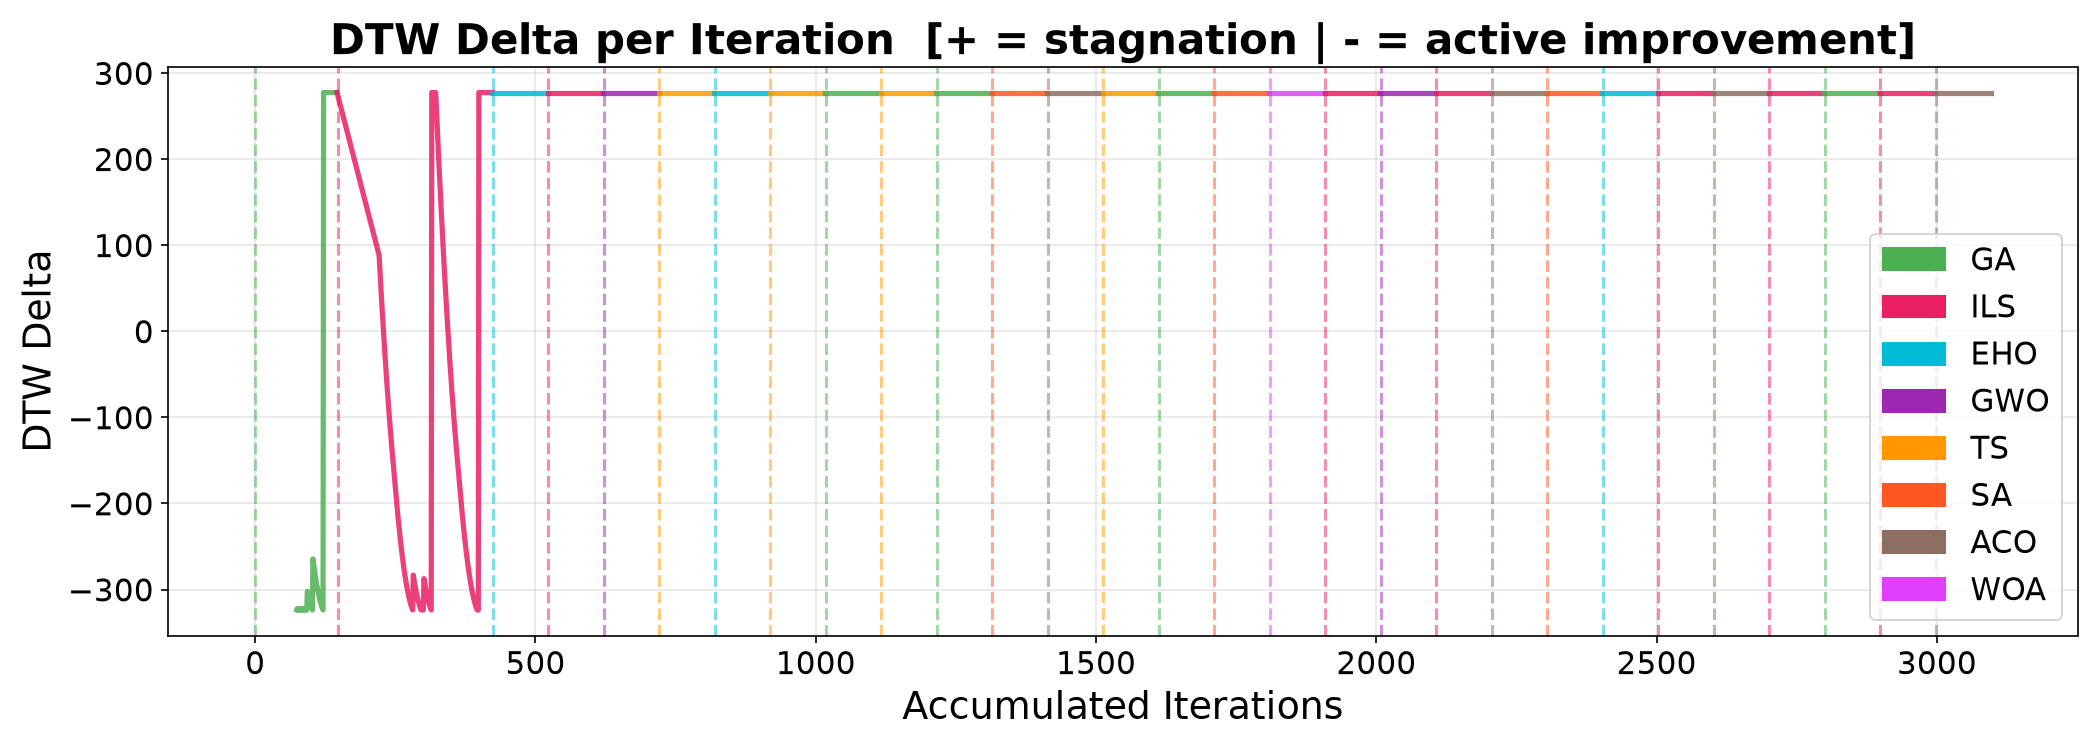
\includegraphics[width=0.32\textwidth]{imagenes_paper/mkp_dtw_3k_mknapcb8_delta.png}}
\caption{Diagnostic suite for instance \textbf{mknapcb8} ($n=250$, $m=30$) under the DTW framework with $T_{\max}=3{,}000$: (a)~final-fitness distribution over $N=31$ runs; (b)~convergence trajectory of the best run; (c)~elastic warping profile $\Delta$.}
\label{fig:mkp-best-cb8}
\end{figure}

% --- mknapcb9: DDTW, 3,000 iterations ---
\begin{figure}[htbp]
\centering
\subfloat[Metaheuristic comparison.]{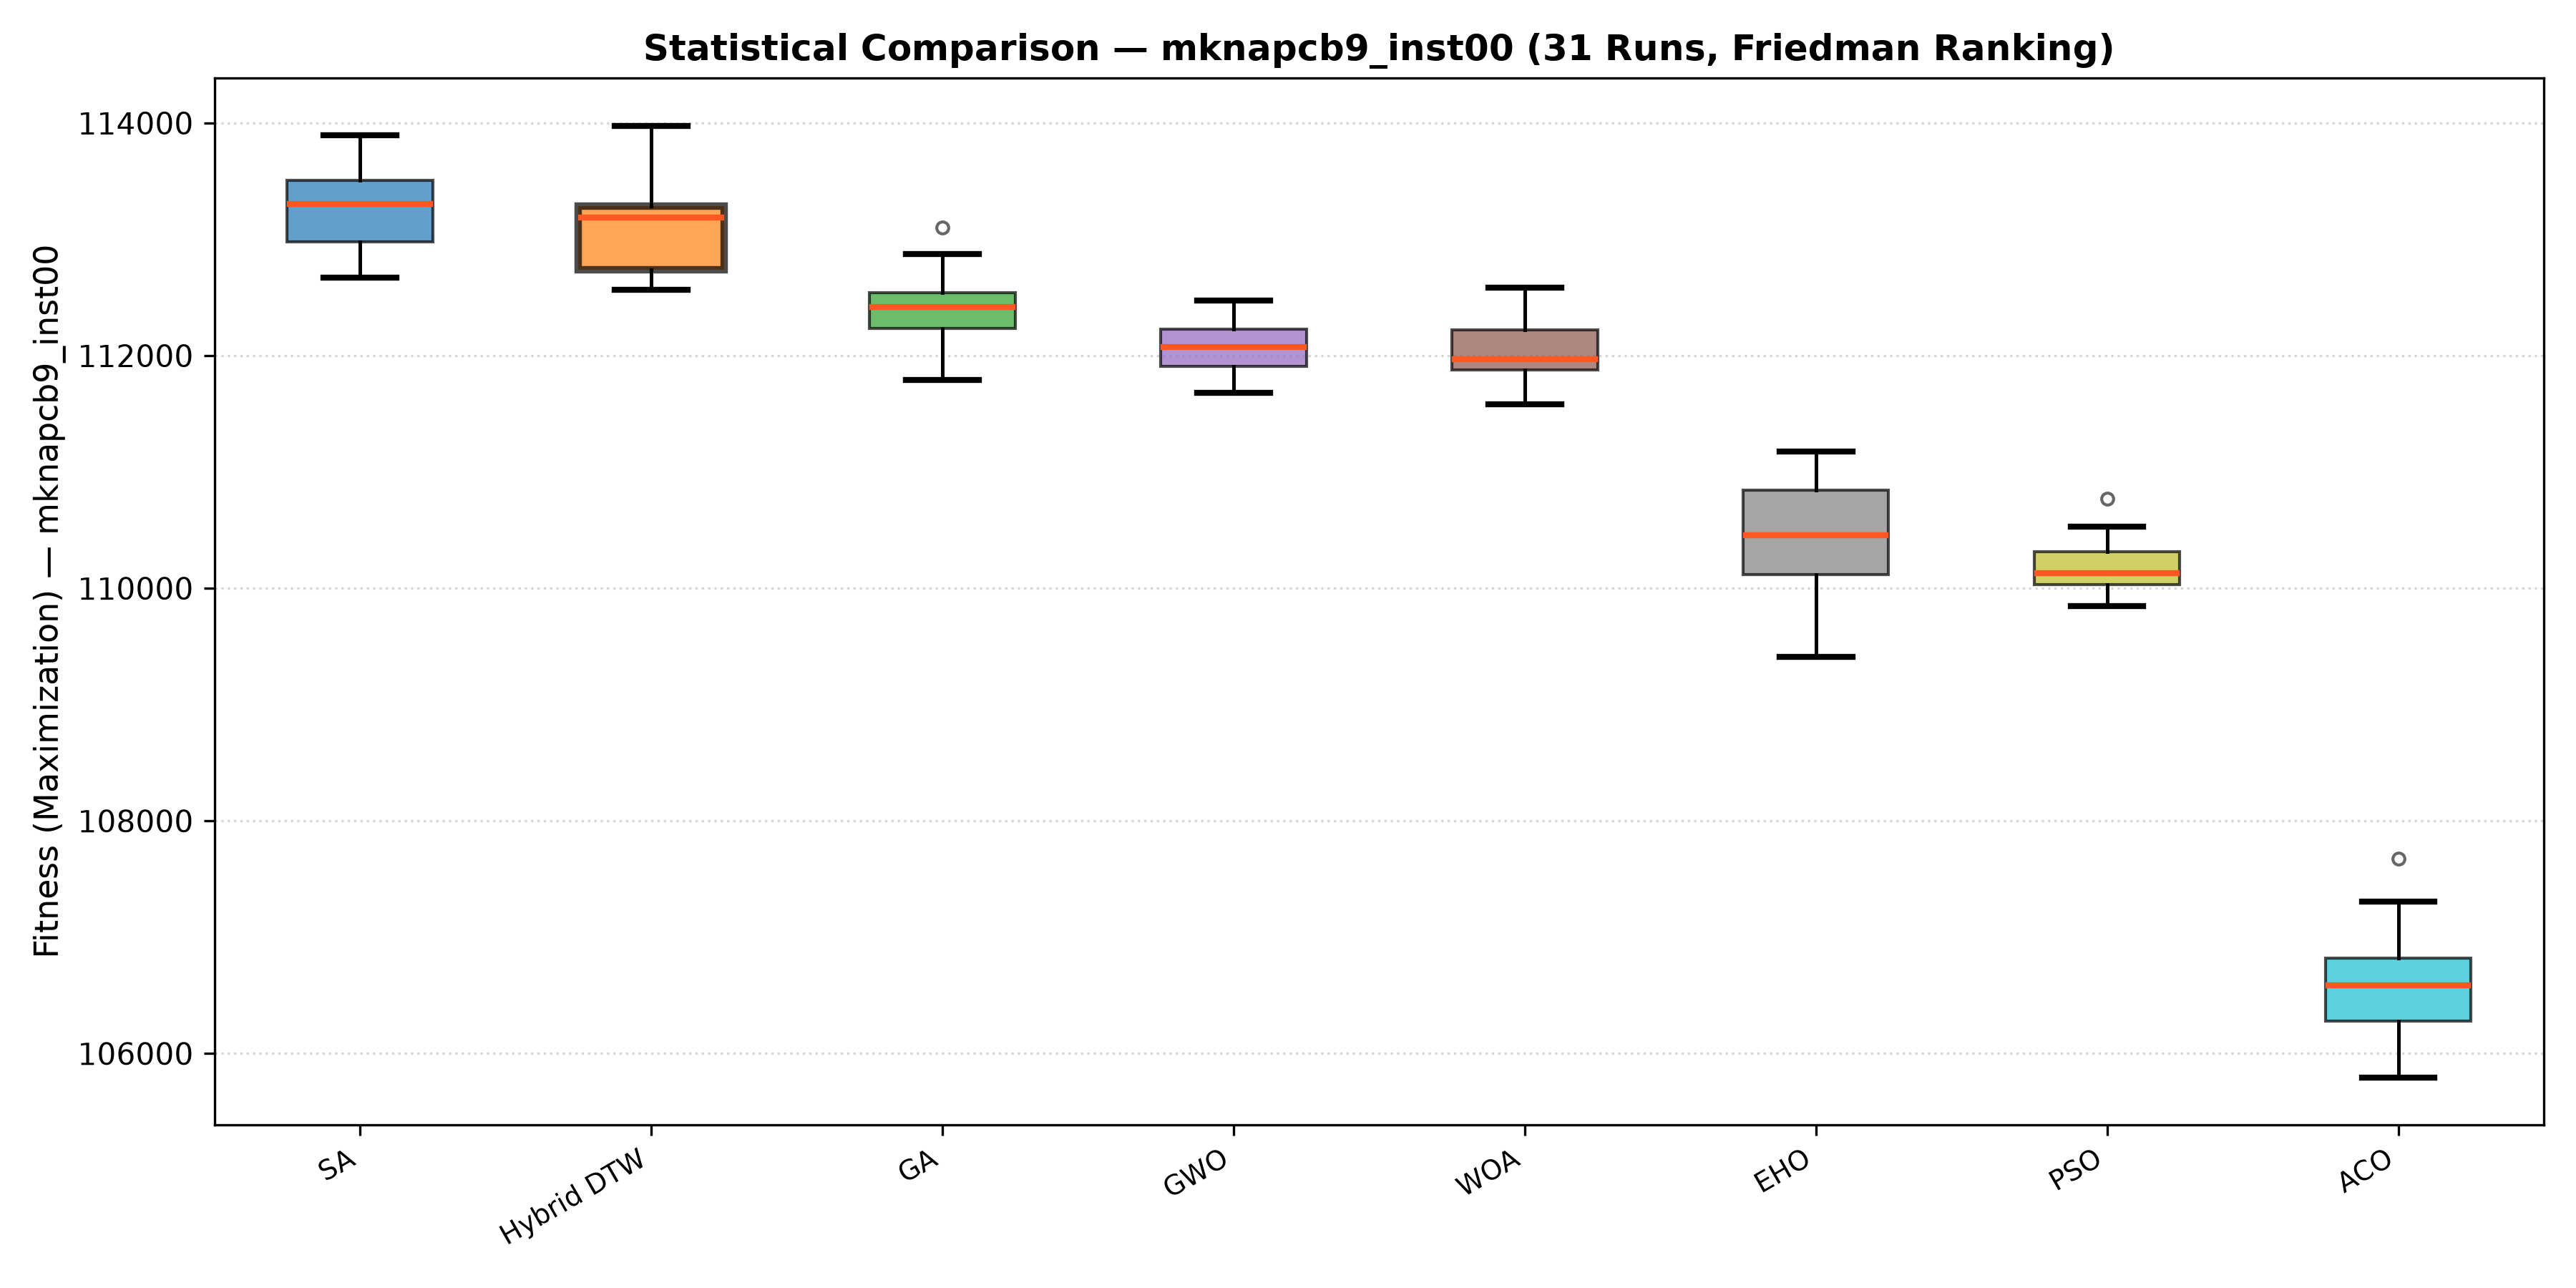
\includegraphics[width=0.32\textwidth]{imagenes_paper/mkp_ddtw_3k_mknapcb9_comparativo_mh.png}}\hfill
\subfloat[Best-run convergence.]{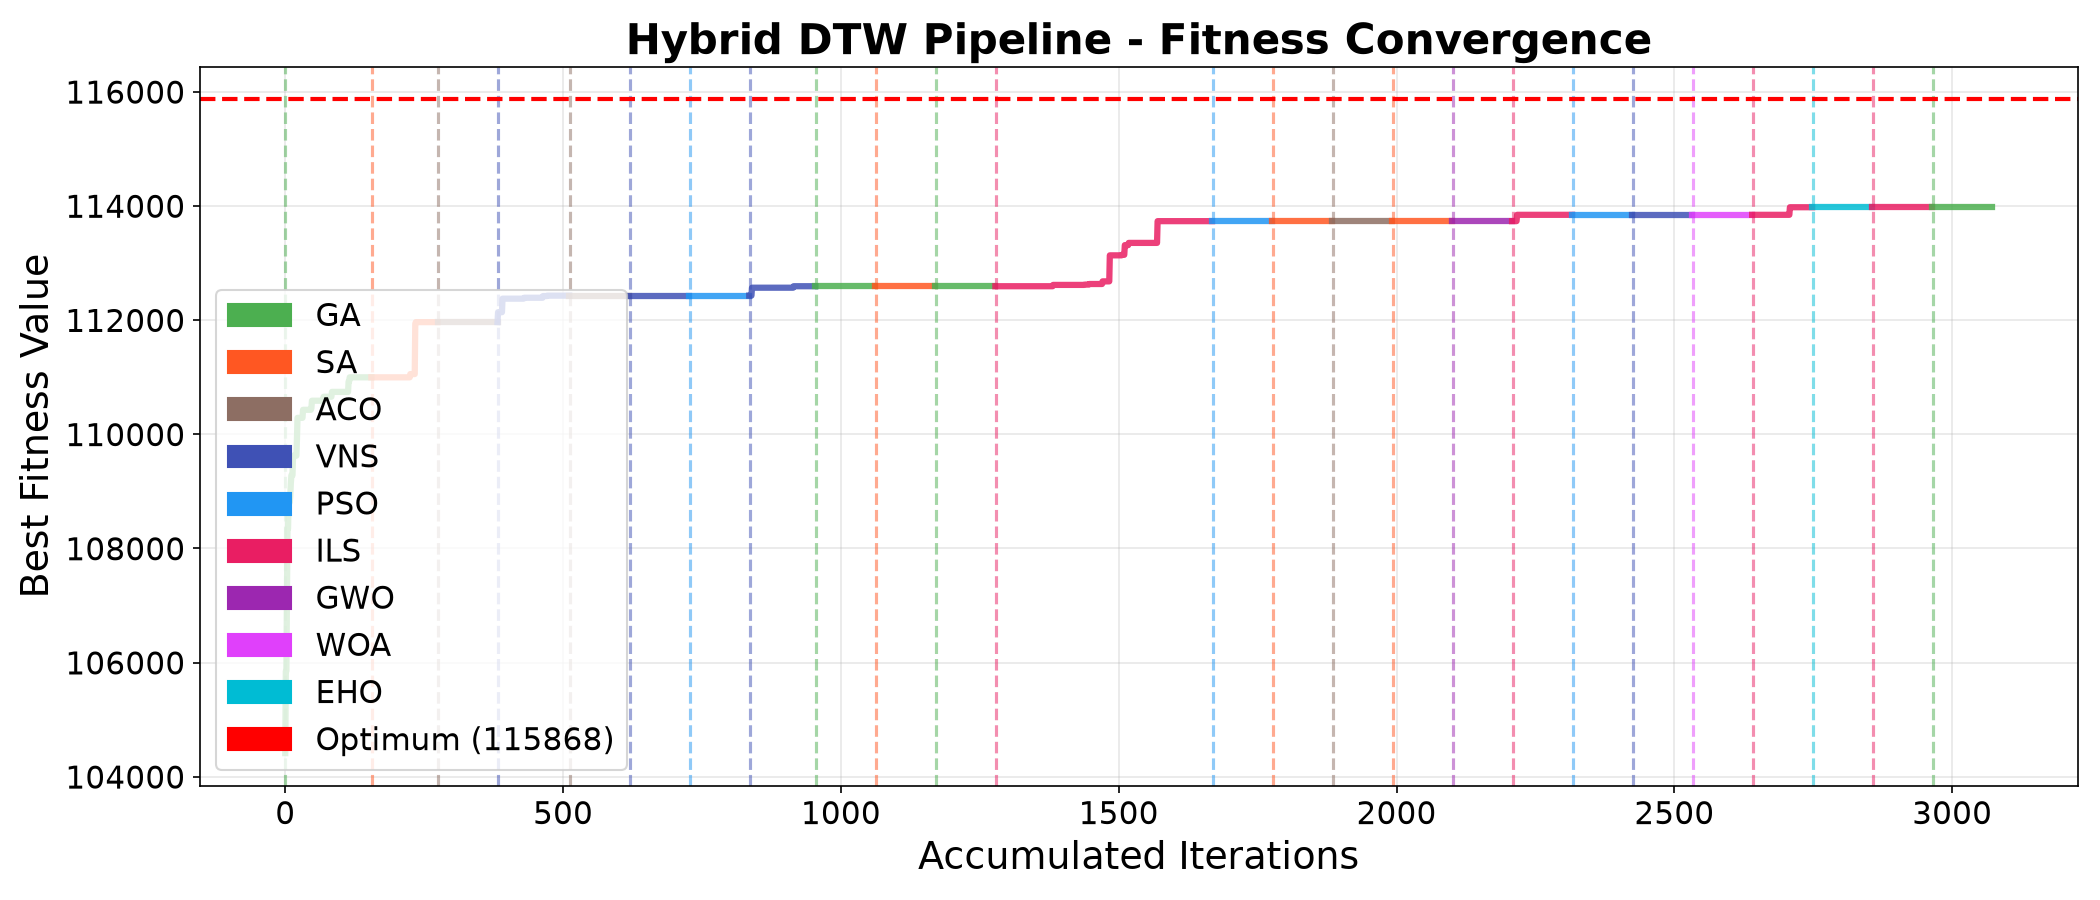
\includegraphics[width=0.32\textwidth]{imagenes_paper/mkp_ddtw_3k_mknapcb9_convergencia.png}}\hfill
\subfloat[Elastic metric $\Delta=D_1-D_2$.]{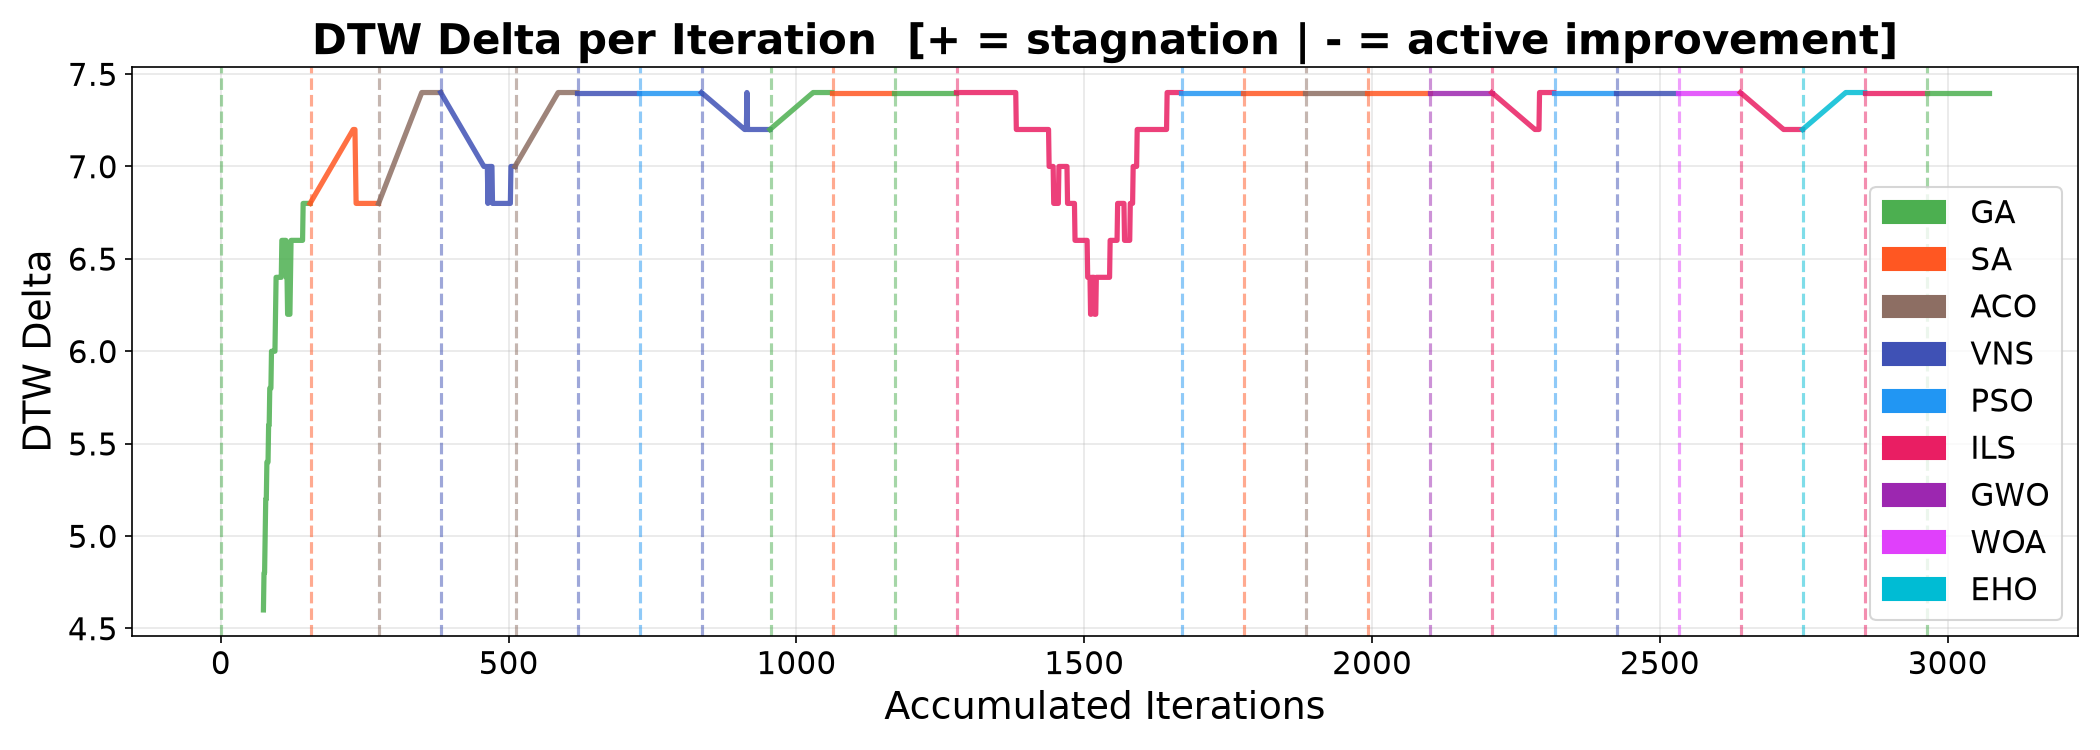
\includegraphics[width=0.32\textwidth]{imagenes_paper/mkp_ddtw_3k_mknapcb9_delta.png}}
\caption{Diagnostic suite for instance \textbf{mknapcb9} ($n=500$, $m=30$) under the DDTW framework with $T_{\max}=3{,}000$: (a)~final-fitness distribution over $N=31$ runs; (b)~convergence trajectory of the best run; (c)~elastic warping profile $\Delta$.}
\label{fig:mkp-best-cb9}
\end{figure}

% Required packages: graphicx, subfig (or subcaption with \subfloat redefined).

% Each figure shows the best-performing framework configuration for the
% corresponding instance, selected by highest mean fitness over 31 runs.
% DTW--3K is best for mknapcb1 and mknapcb3--mknapcb8;
% DDTW--3K is best for mknapcb2 and mknapcb9.

Figures~\ref{fig:mkp-best-cb1}--\ref{fig:mkp-best-cb9} present the
diagnostic suite for each of the nine Chu--Beasley MKP instances under its
best-performing framework configuration, selected by highest mean fitness
over the 31 runs, with corresponding executions treated as paired. DTW with $T_{\max}=3{,}000$ achieved the
highest mean in seven instances (mknapcb1 and mknapcb3--mknapcb8), while
DDTW with $T_{\max}=3{,}000$ was superior for mknapcb2 and mknapcb9.
Each figure comprises three panels: (a)~a box-plot comparing the
final-fitness distributions of the hybrid framework against the standalone
metaheuristics over the 31 runs, allowing visual assessment of both central
tendency and dispersion; (b)~the convergence trajectory of the best run,
showing the evolution of the incumbent fitness along with the solver
transitions triggered by the stagnation monitor; and (c)~the elastic
warping profile $\Delta = D_1 - D_2$, where positive values indicate
detected stagnation phases and negative values correspond to periods of
active improvement.

% --- mknapcb1: DTW, 3,000 iterations ---
\begin{figure}[htbp]
\centering
\subfloat[Metaheuristic comparison.]{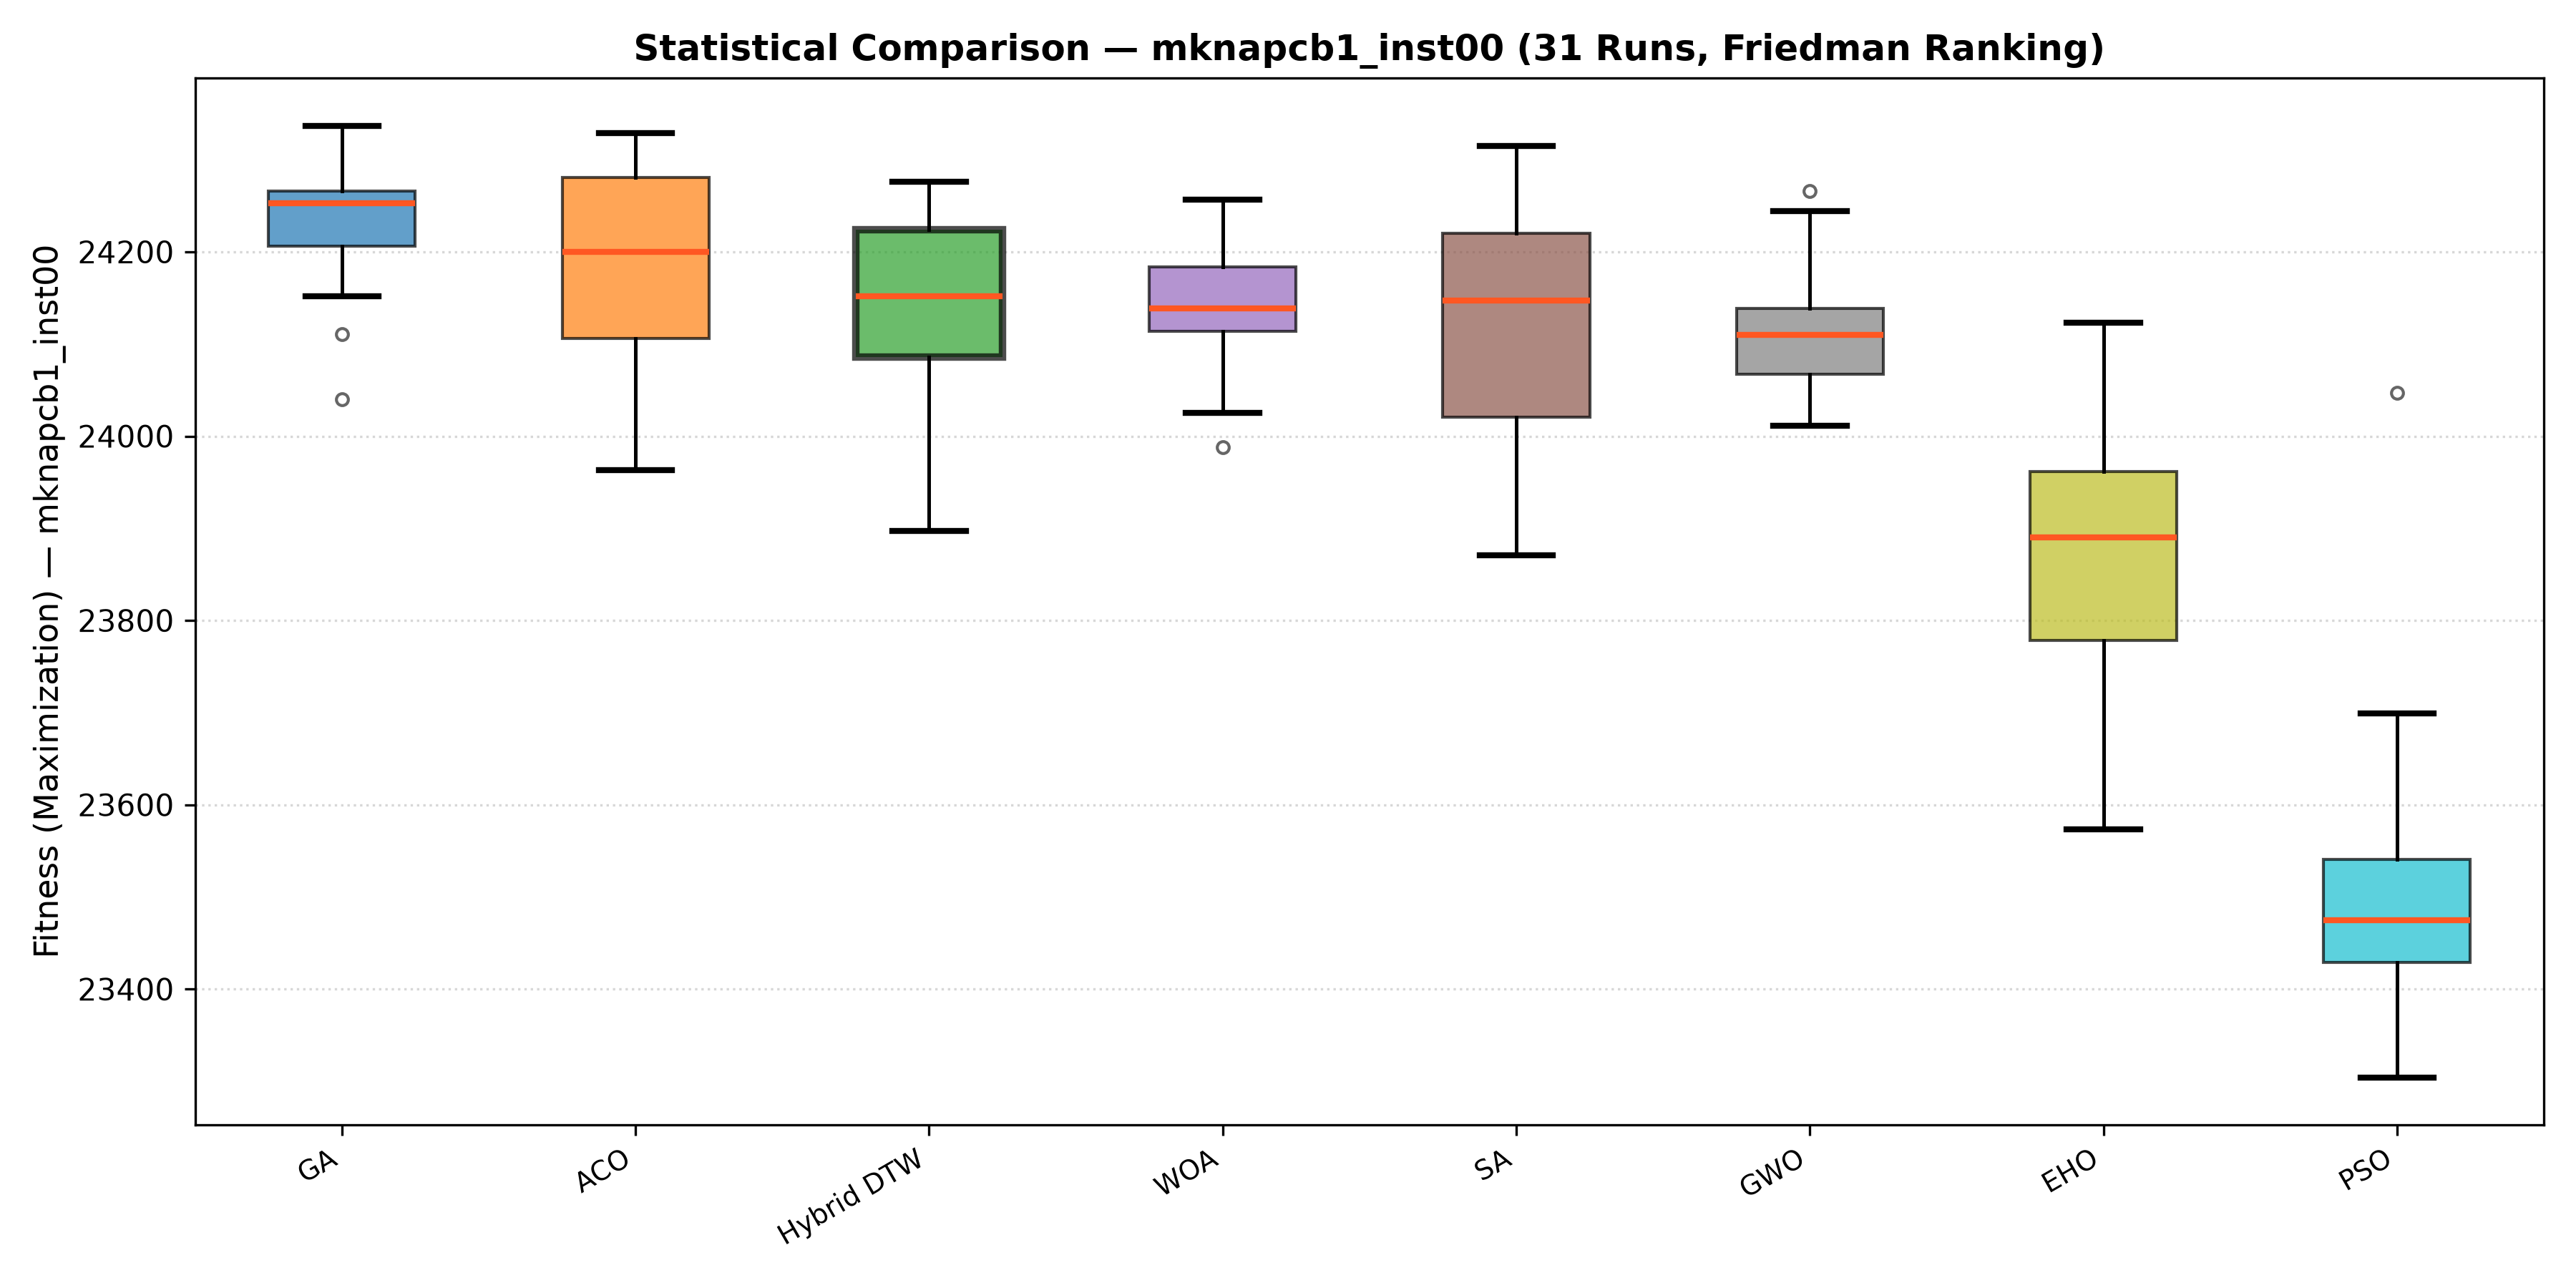
\includegraphics[width=0.32\textwidth]{imagenes_paper/mkp_dtw_3k_mknapcb1_comparativo_mh.png}}\hfill
\subfloat[Best-run convergence.]{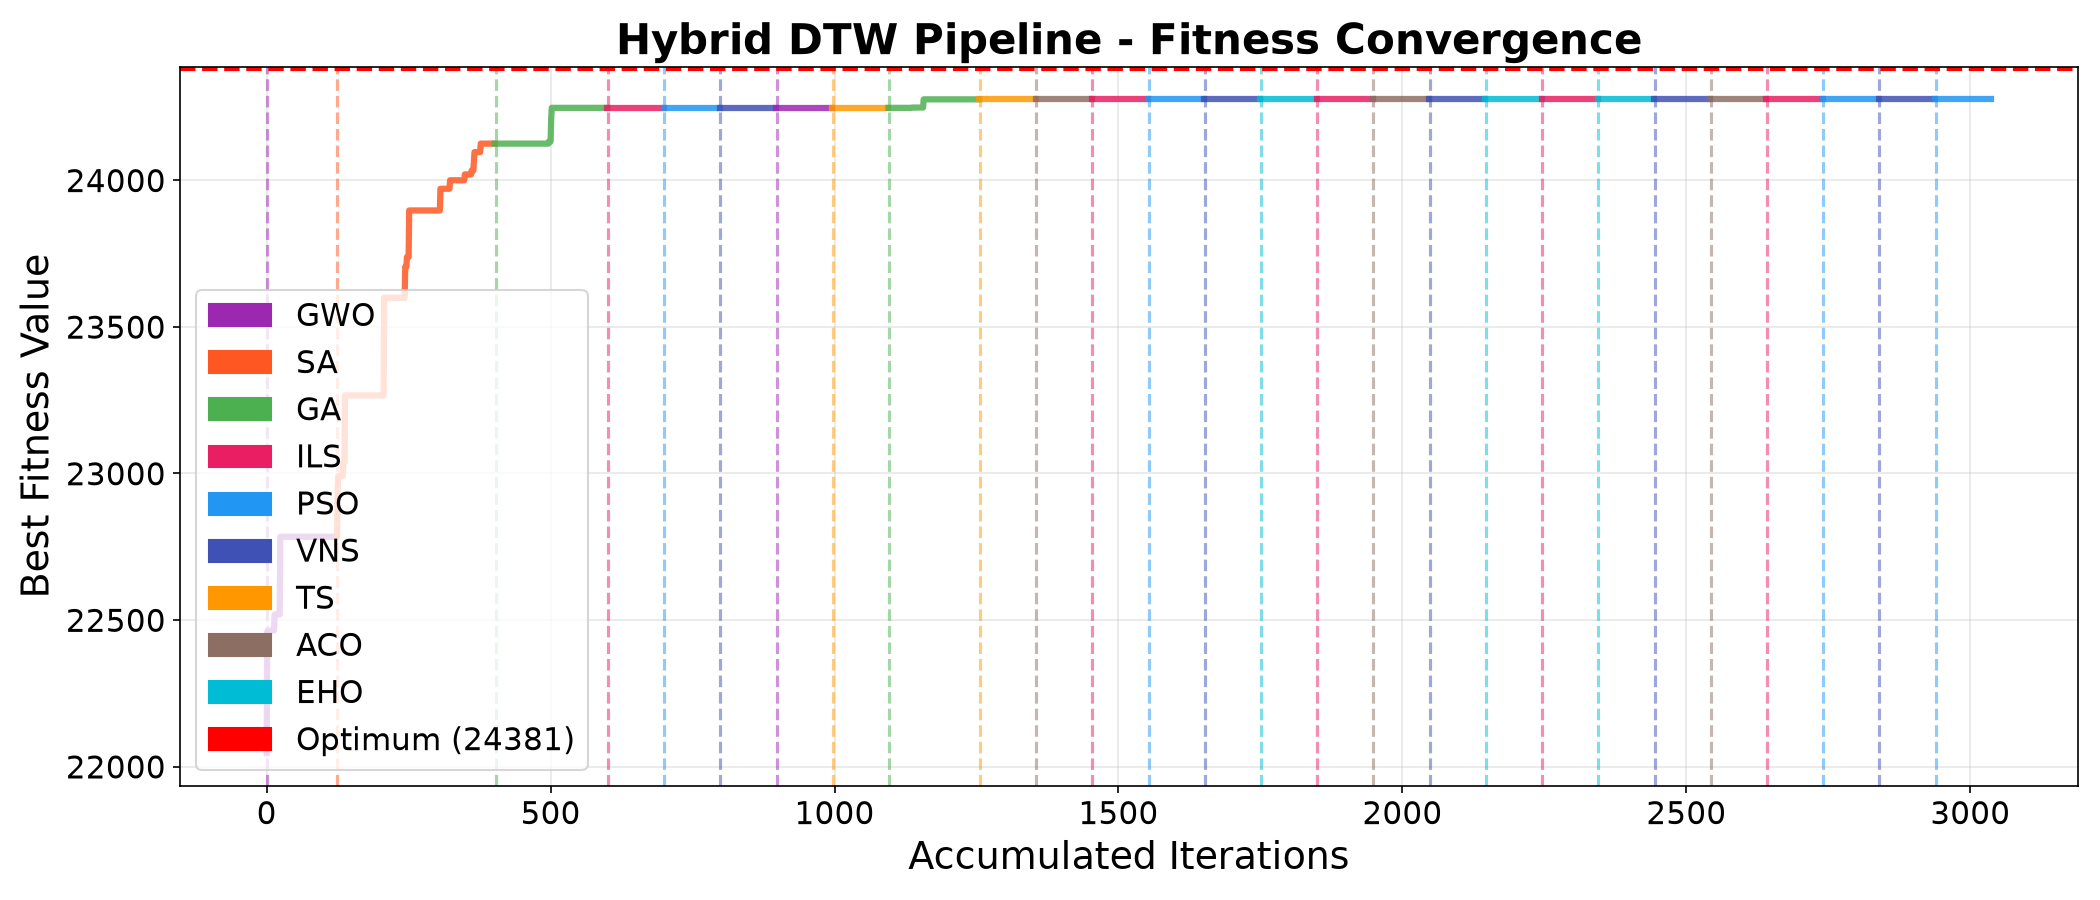
\includegraphics[width=0.32\textwidth]{imagenes_paper/mkp_dtw_3k_mknapcb1_convergencia.png}}\hfill
\subfloat[Elastic metric $\Delta=D_1-D_2$.]{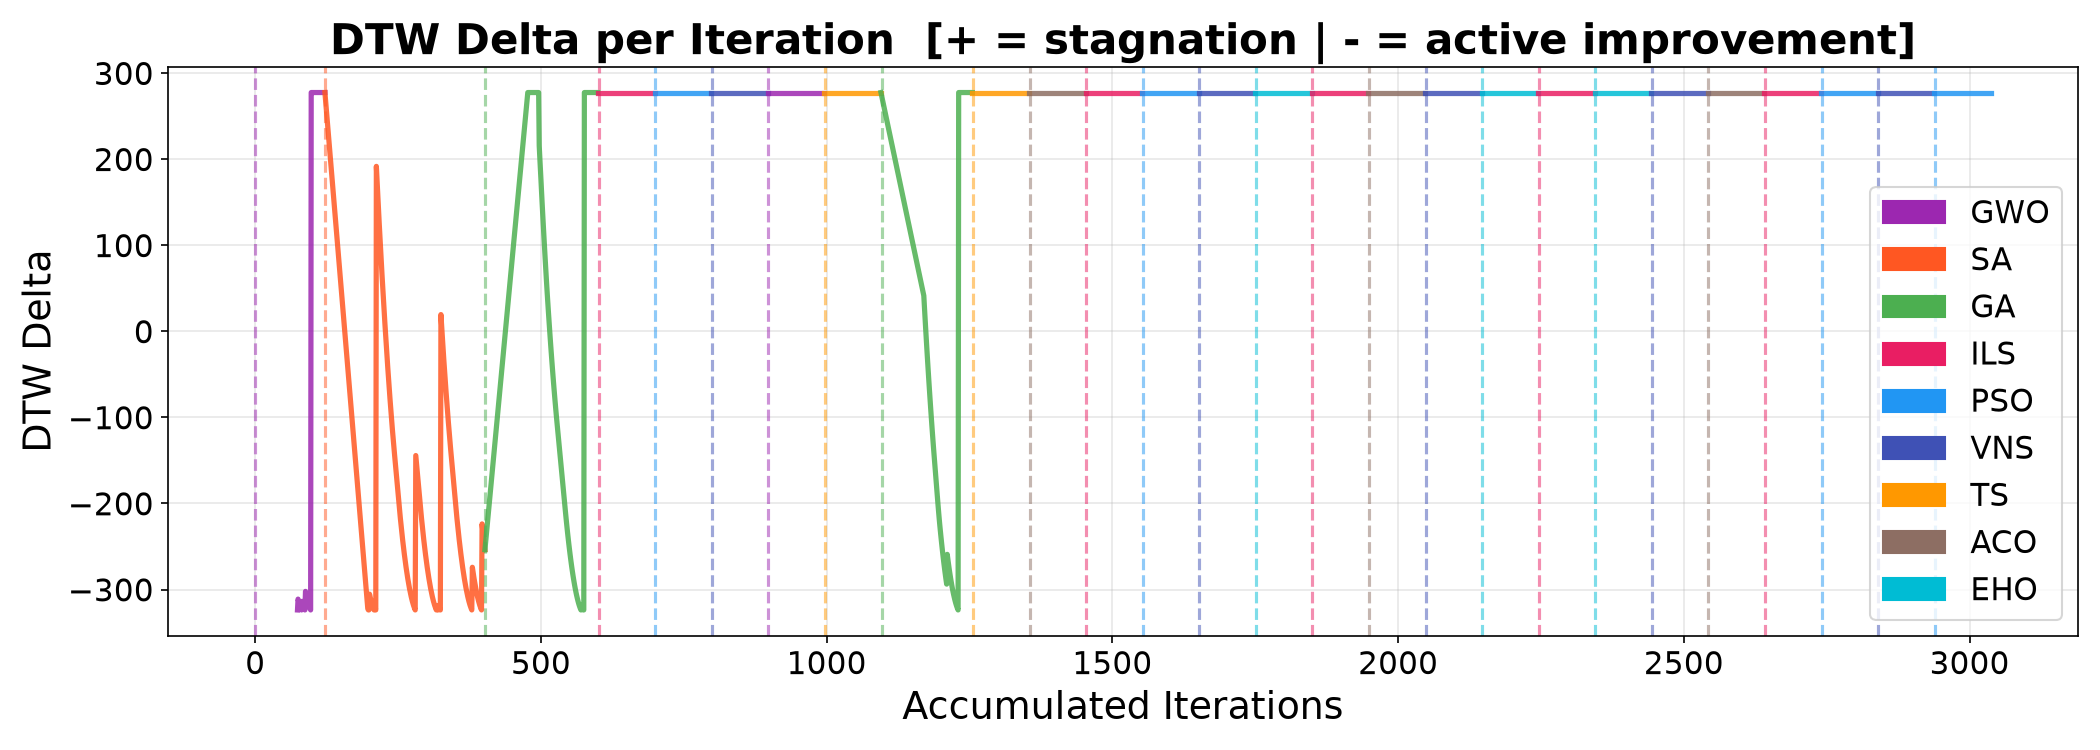
\includegraphics[width=0.32\textwidth]{imagenes_paper/mkp_dtw_3k_mknapcb1_delta.png}}
\caption{Diagnostic suite for instance \textbf{mknapcb1} ($n=100$, $m=5$) under the DTW framework with $T_{\max}=3{,}000$: (a)~final-fitness distribution over $N=31$ runs; (b)~convergence trajectory of the best run; (c)~elastic warping profile $\Delta$.}
\label{fig:mkp-best-cb1}
\end{figure}

% --- mknapcb2: DDTW, 3,000 iterations ---
\begin{figure}[htbp]
\centering
\subfloat[Metaheuristic comparison.]{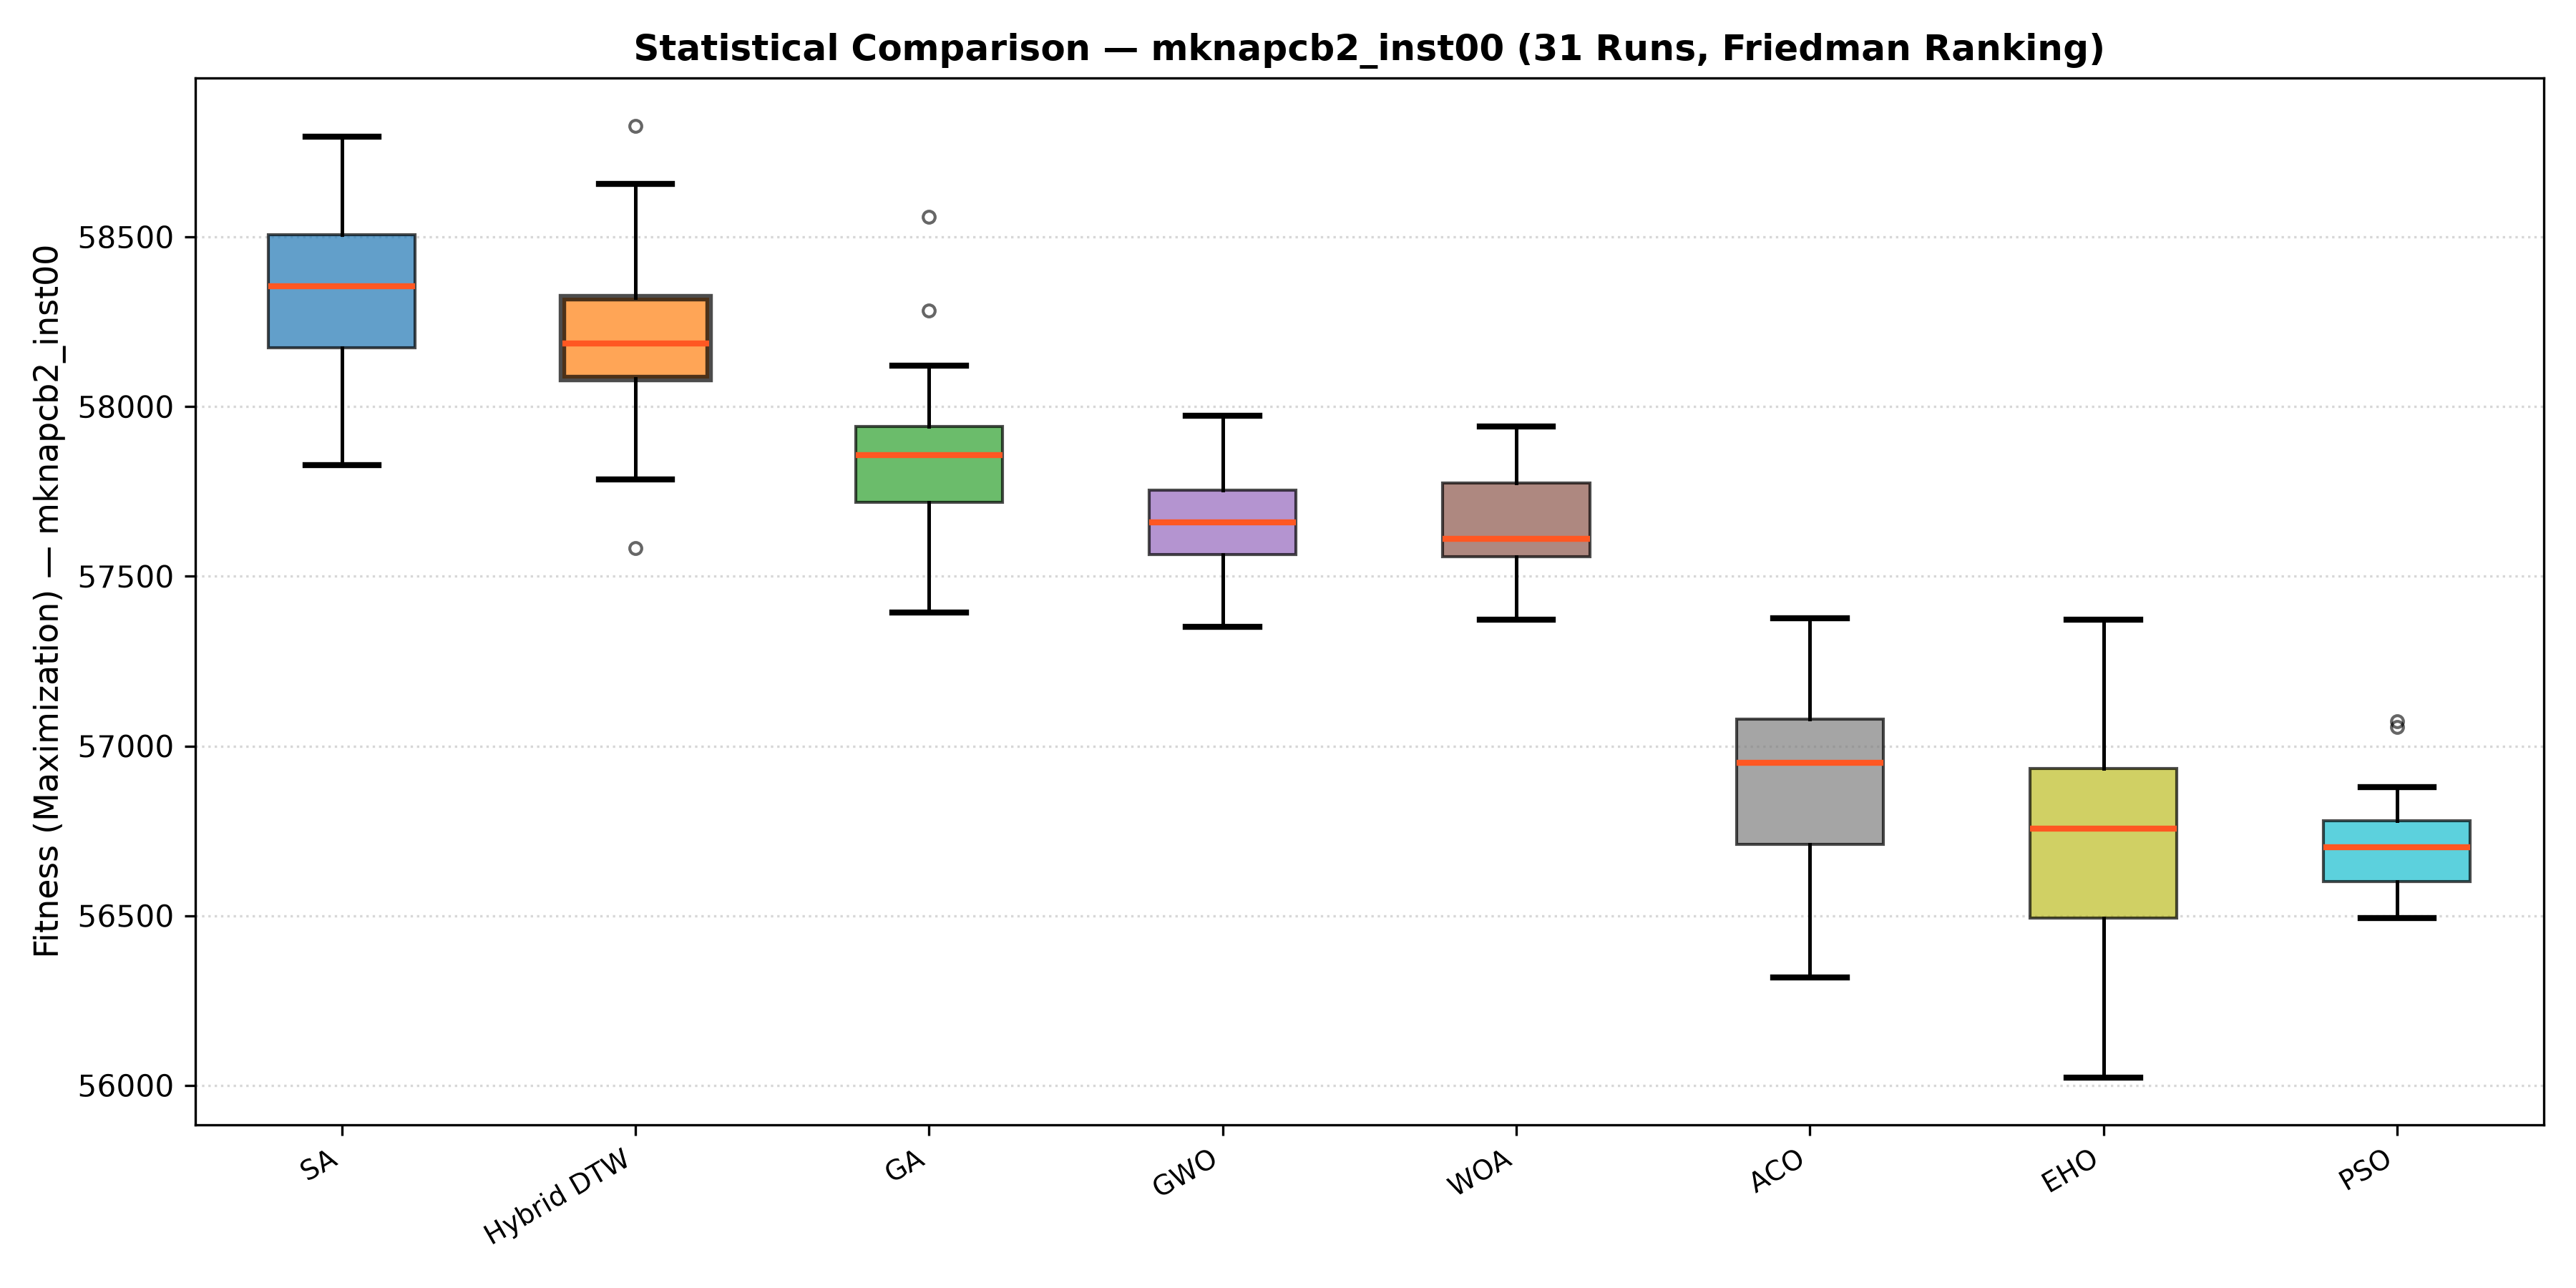
\includegraphics[width=0.32\textwidth]{imagenes_paper/mkp_ddtw_3k_mknapcb2_comparativo_mh.png}}\hfill
\subfloat[Best-run convergence.]{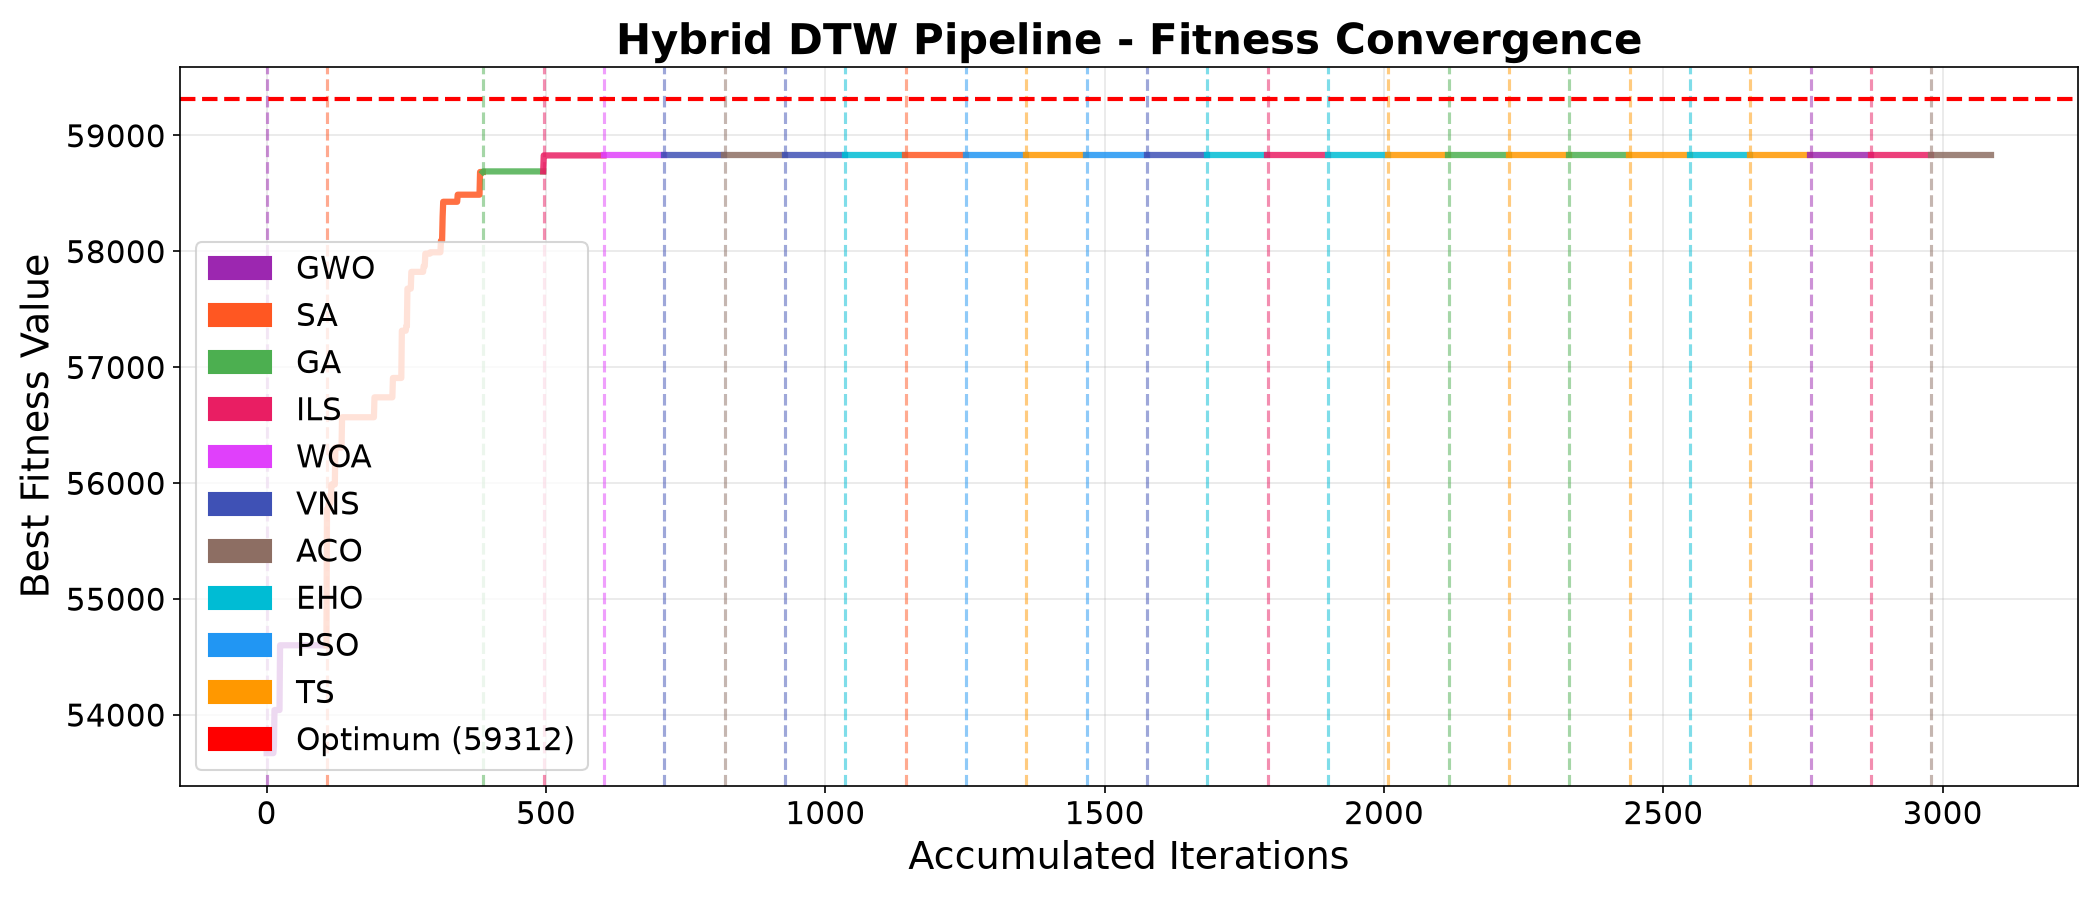
\includegraphics[width=0.32\textwidth]{imagenes_paper/mkp_ddtw_3k_mknapcb2_convergencia.png}}\hfill
\subfloat[Elastic metric $\Delta=D_1-D_2$.]{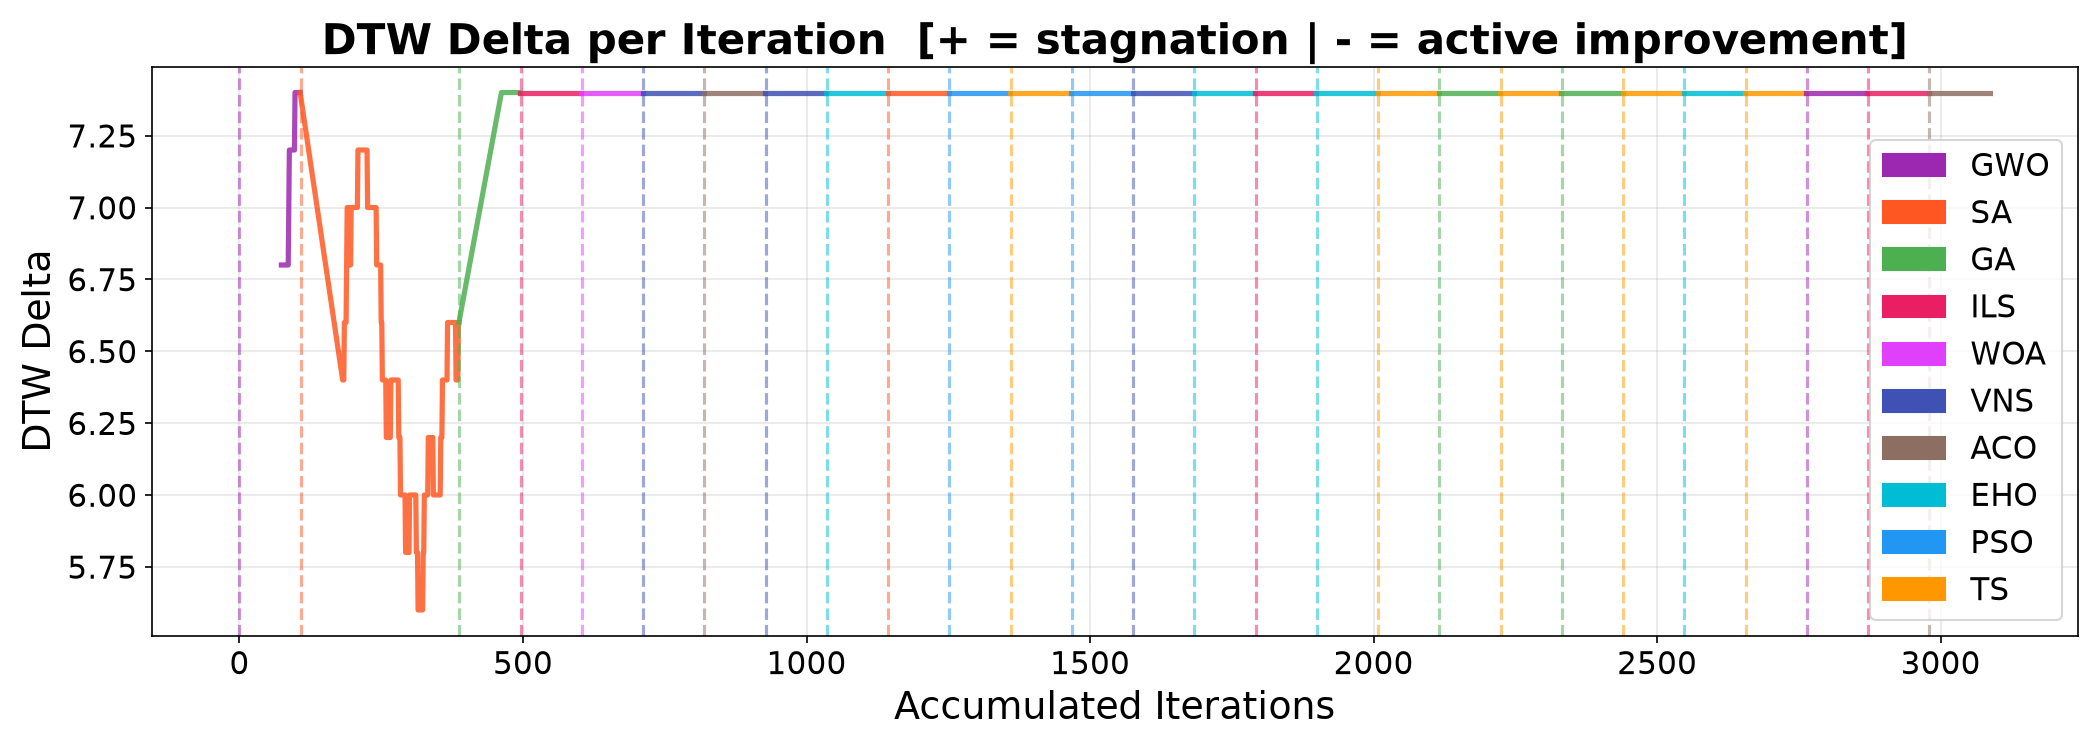
\includegraphics[width=0.32\textwidth]{imagenes_paper/mkp_ddtw_3k_mknapcb2_delta.png}}
\caption{Diagnostic suite for instance \textbf{mknapcb2} ($n=250$, $m=5$) under the DDTW framework with $T_{\max}=3{,}000$: (a)~final-fitness distribution over $N=31$ runs; (b)~convergence trajectory of the best run; (c)~elastic warping profile $\Delta$.}
\label{fig:mkp-best-cb2}
\end{figure}

% --- mknapcb3: DTW, 3,000 iterations ---
\begin{figure}[htbp]
\centering
\subfloat[Metaheuristic comparison.]{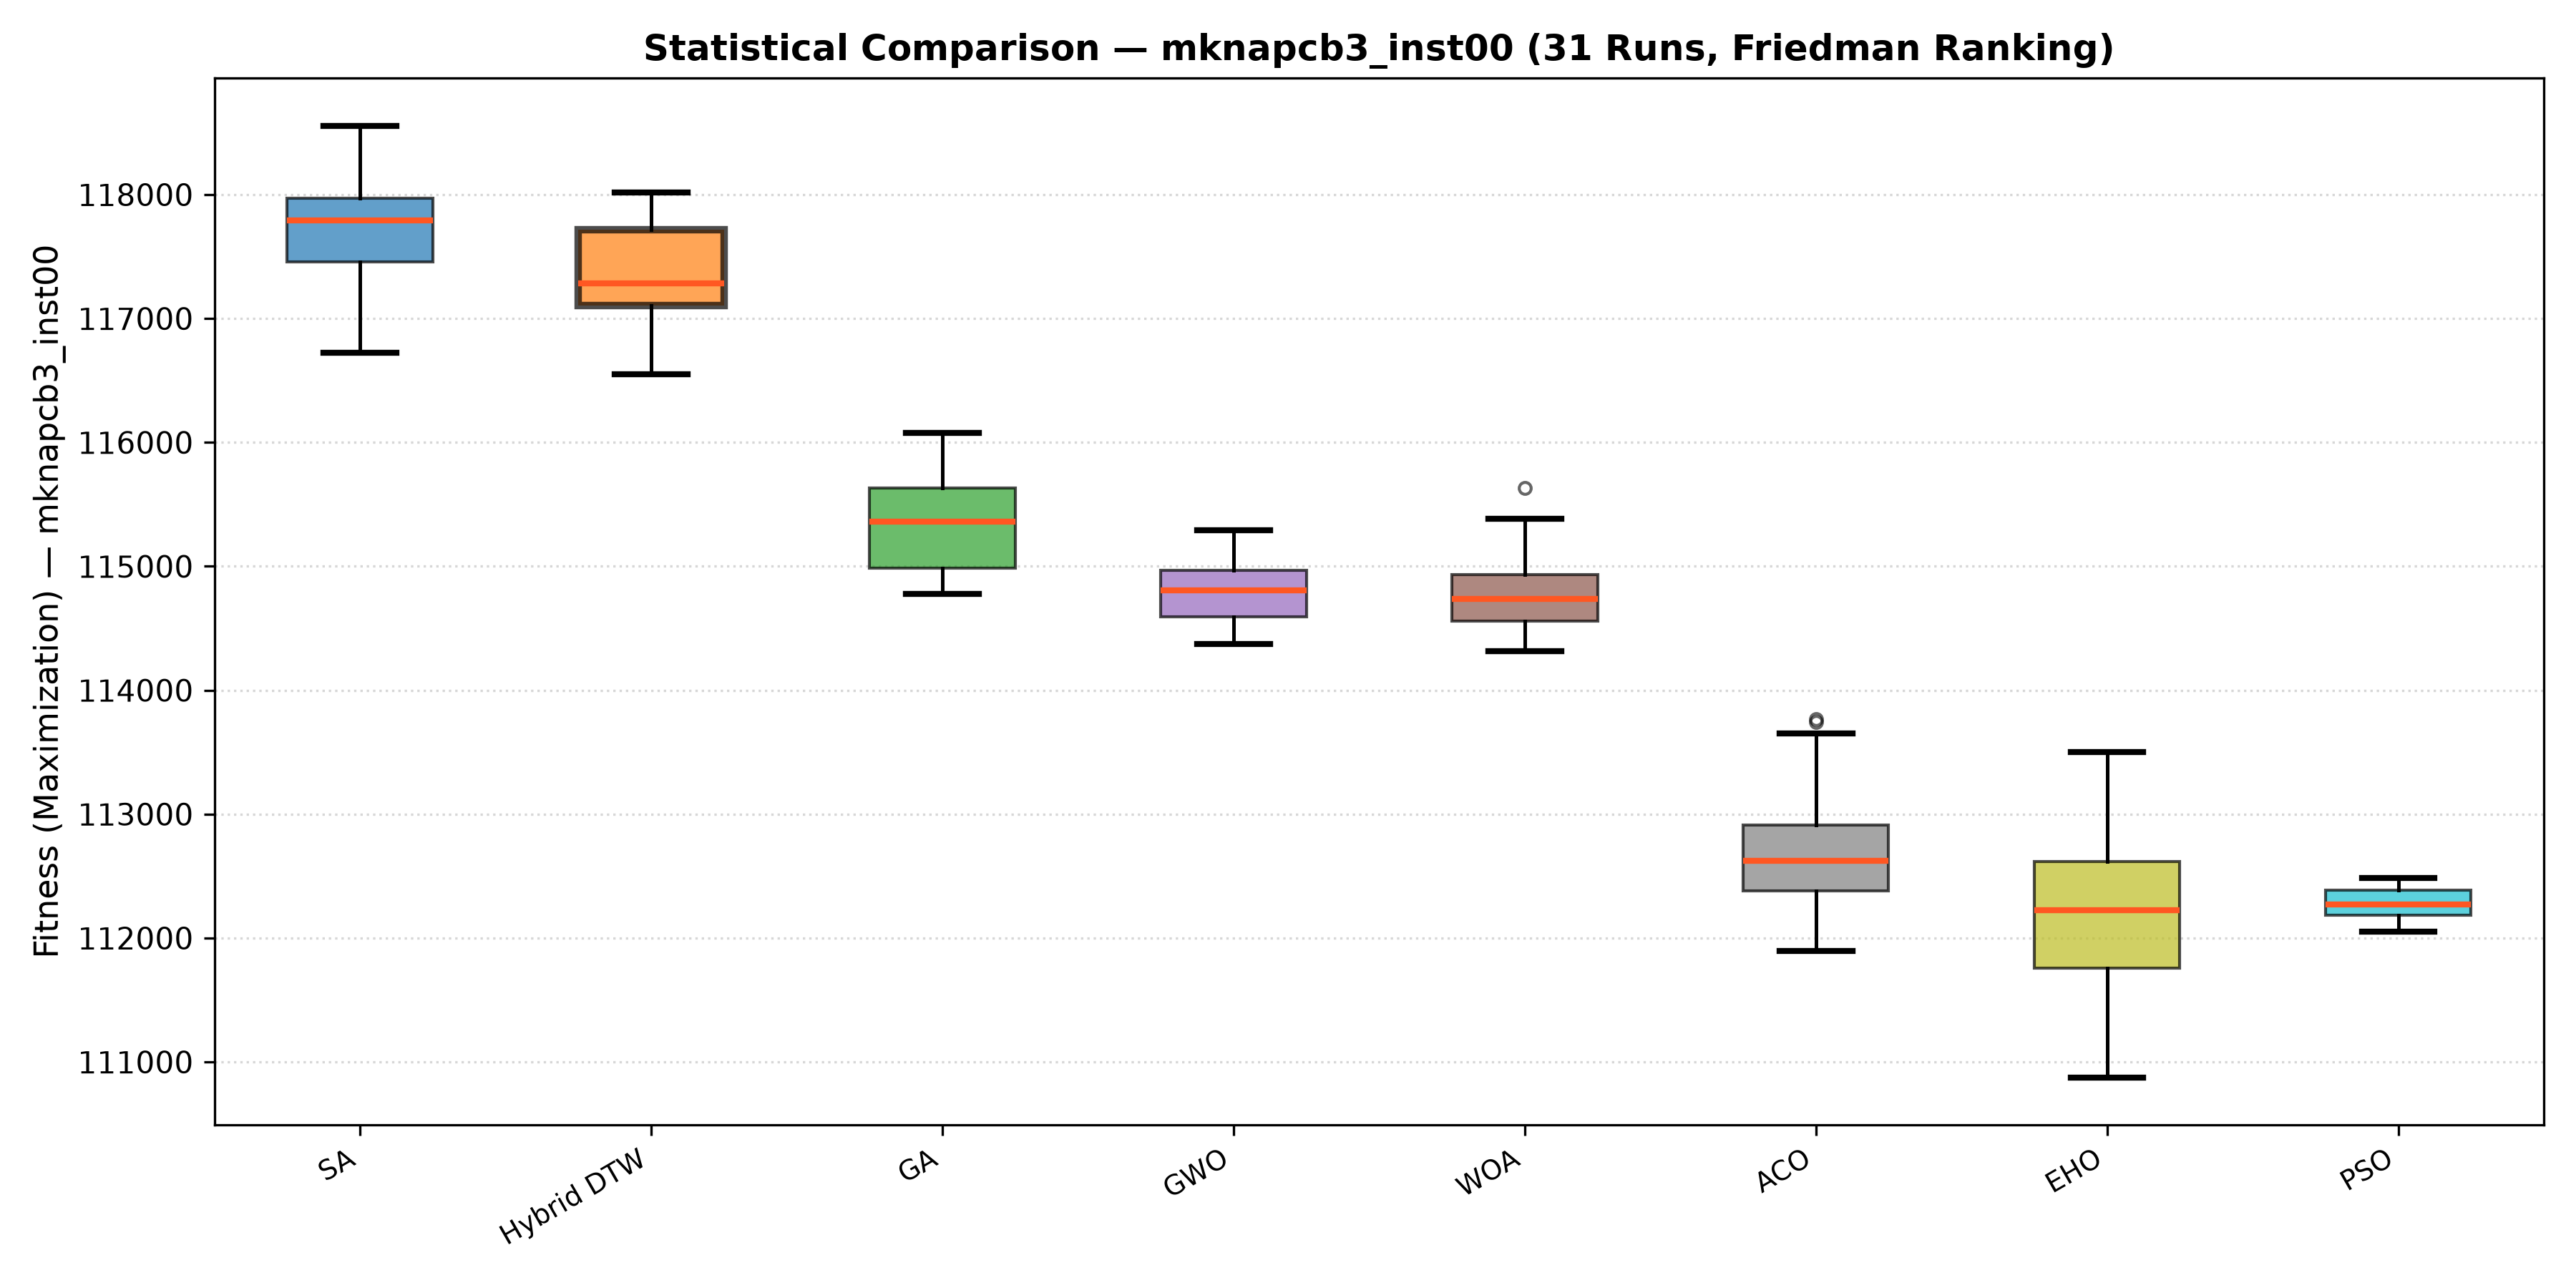
\includegraphics[width=0.32\textwidth]{imagenes_paper/mkp_dtw_3k_mknapcb3_comparativo_mh.png}}\hfill
\subfloat[Best-run convergence.]{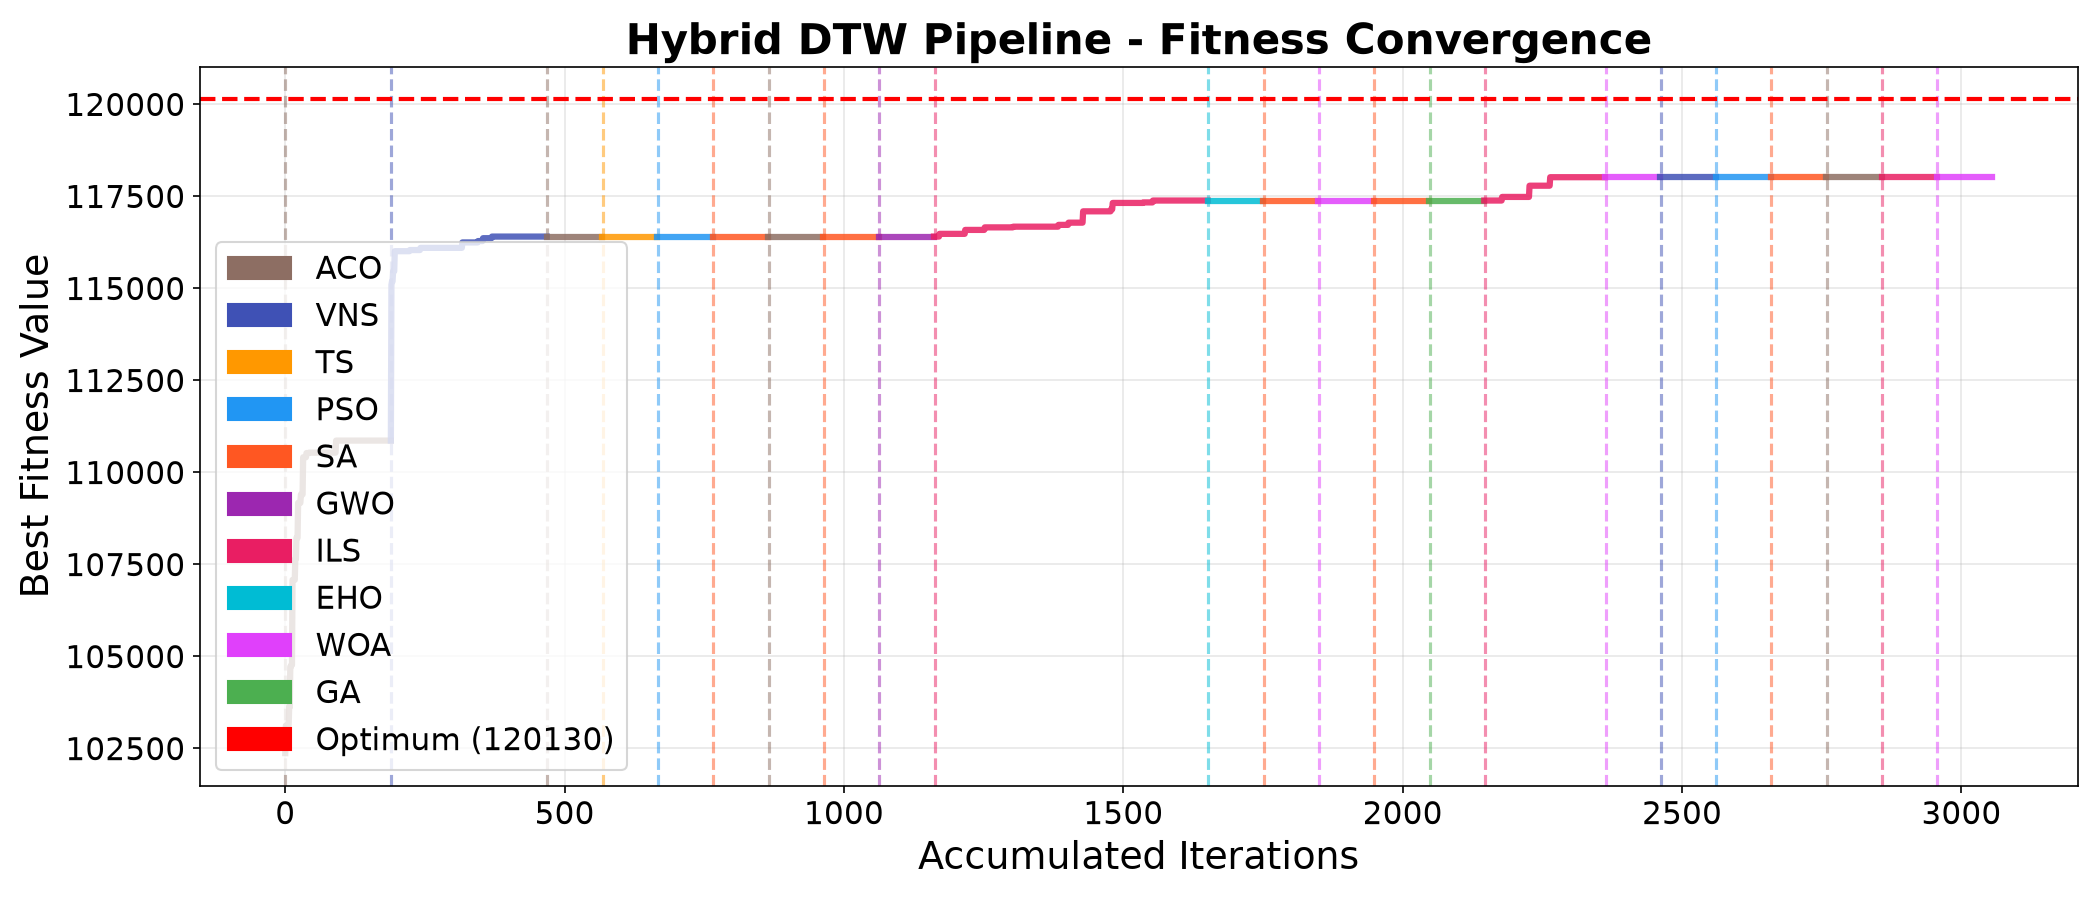
\includegraphics[width=0.32\textwidth]{imagenes_paper/mkp_dtw_3k_mknapcb3_convergencia.png}}\hfill
\subfloat[Elastic metric $\Delta=D_1-D_2$.]{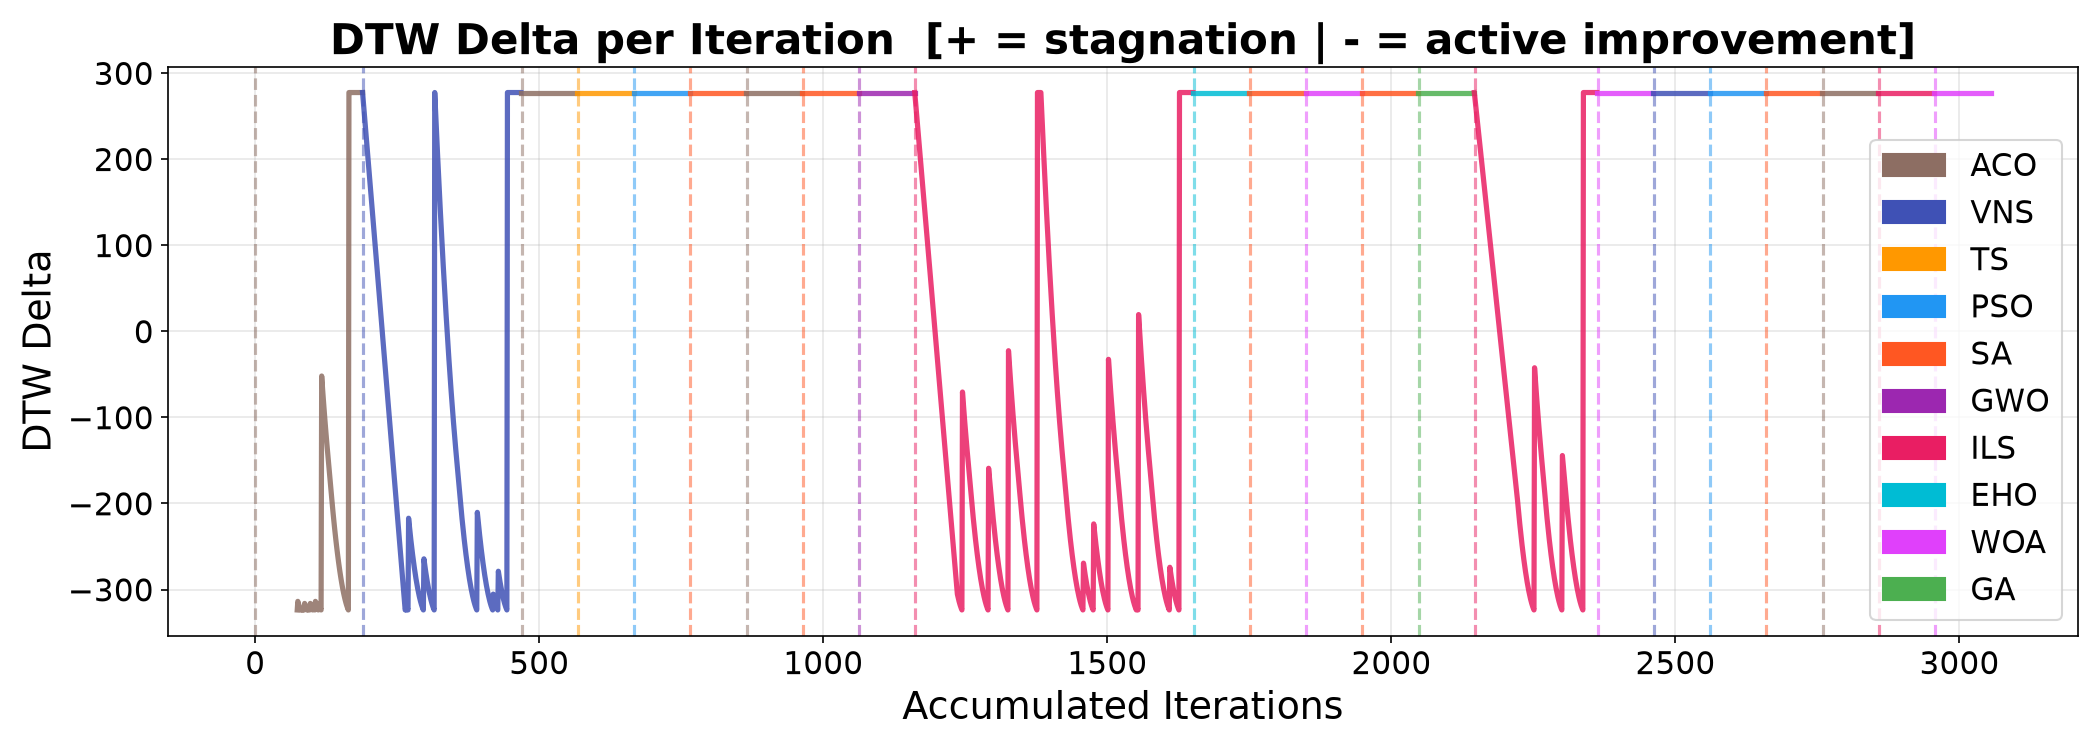
\includegraphics[width=0.32\textwidth]{imagenes_paper/mkp_dtw_3k_mknapcb3_delta.png}}
\caption{Diagnostic suite for instance \textbf{mknapcb3} ($n=500$, $m=5$) under the DTW framework with $T_{\max}=3{,}000$: (a)~final-fitness distribution over $N=31$ runs; (b)~convergence trajectory of the best run; (c)~elastic warping profile $\Delta$.}
\label{fig:mkp-best-cb3}
\end{figure}

% --- mknapcb4: DTW, 3,000 iterations ---
\begin{figure}[htbp]
\centering
\subfloat[Metaheuristic comparison.]{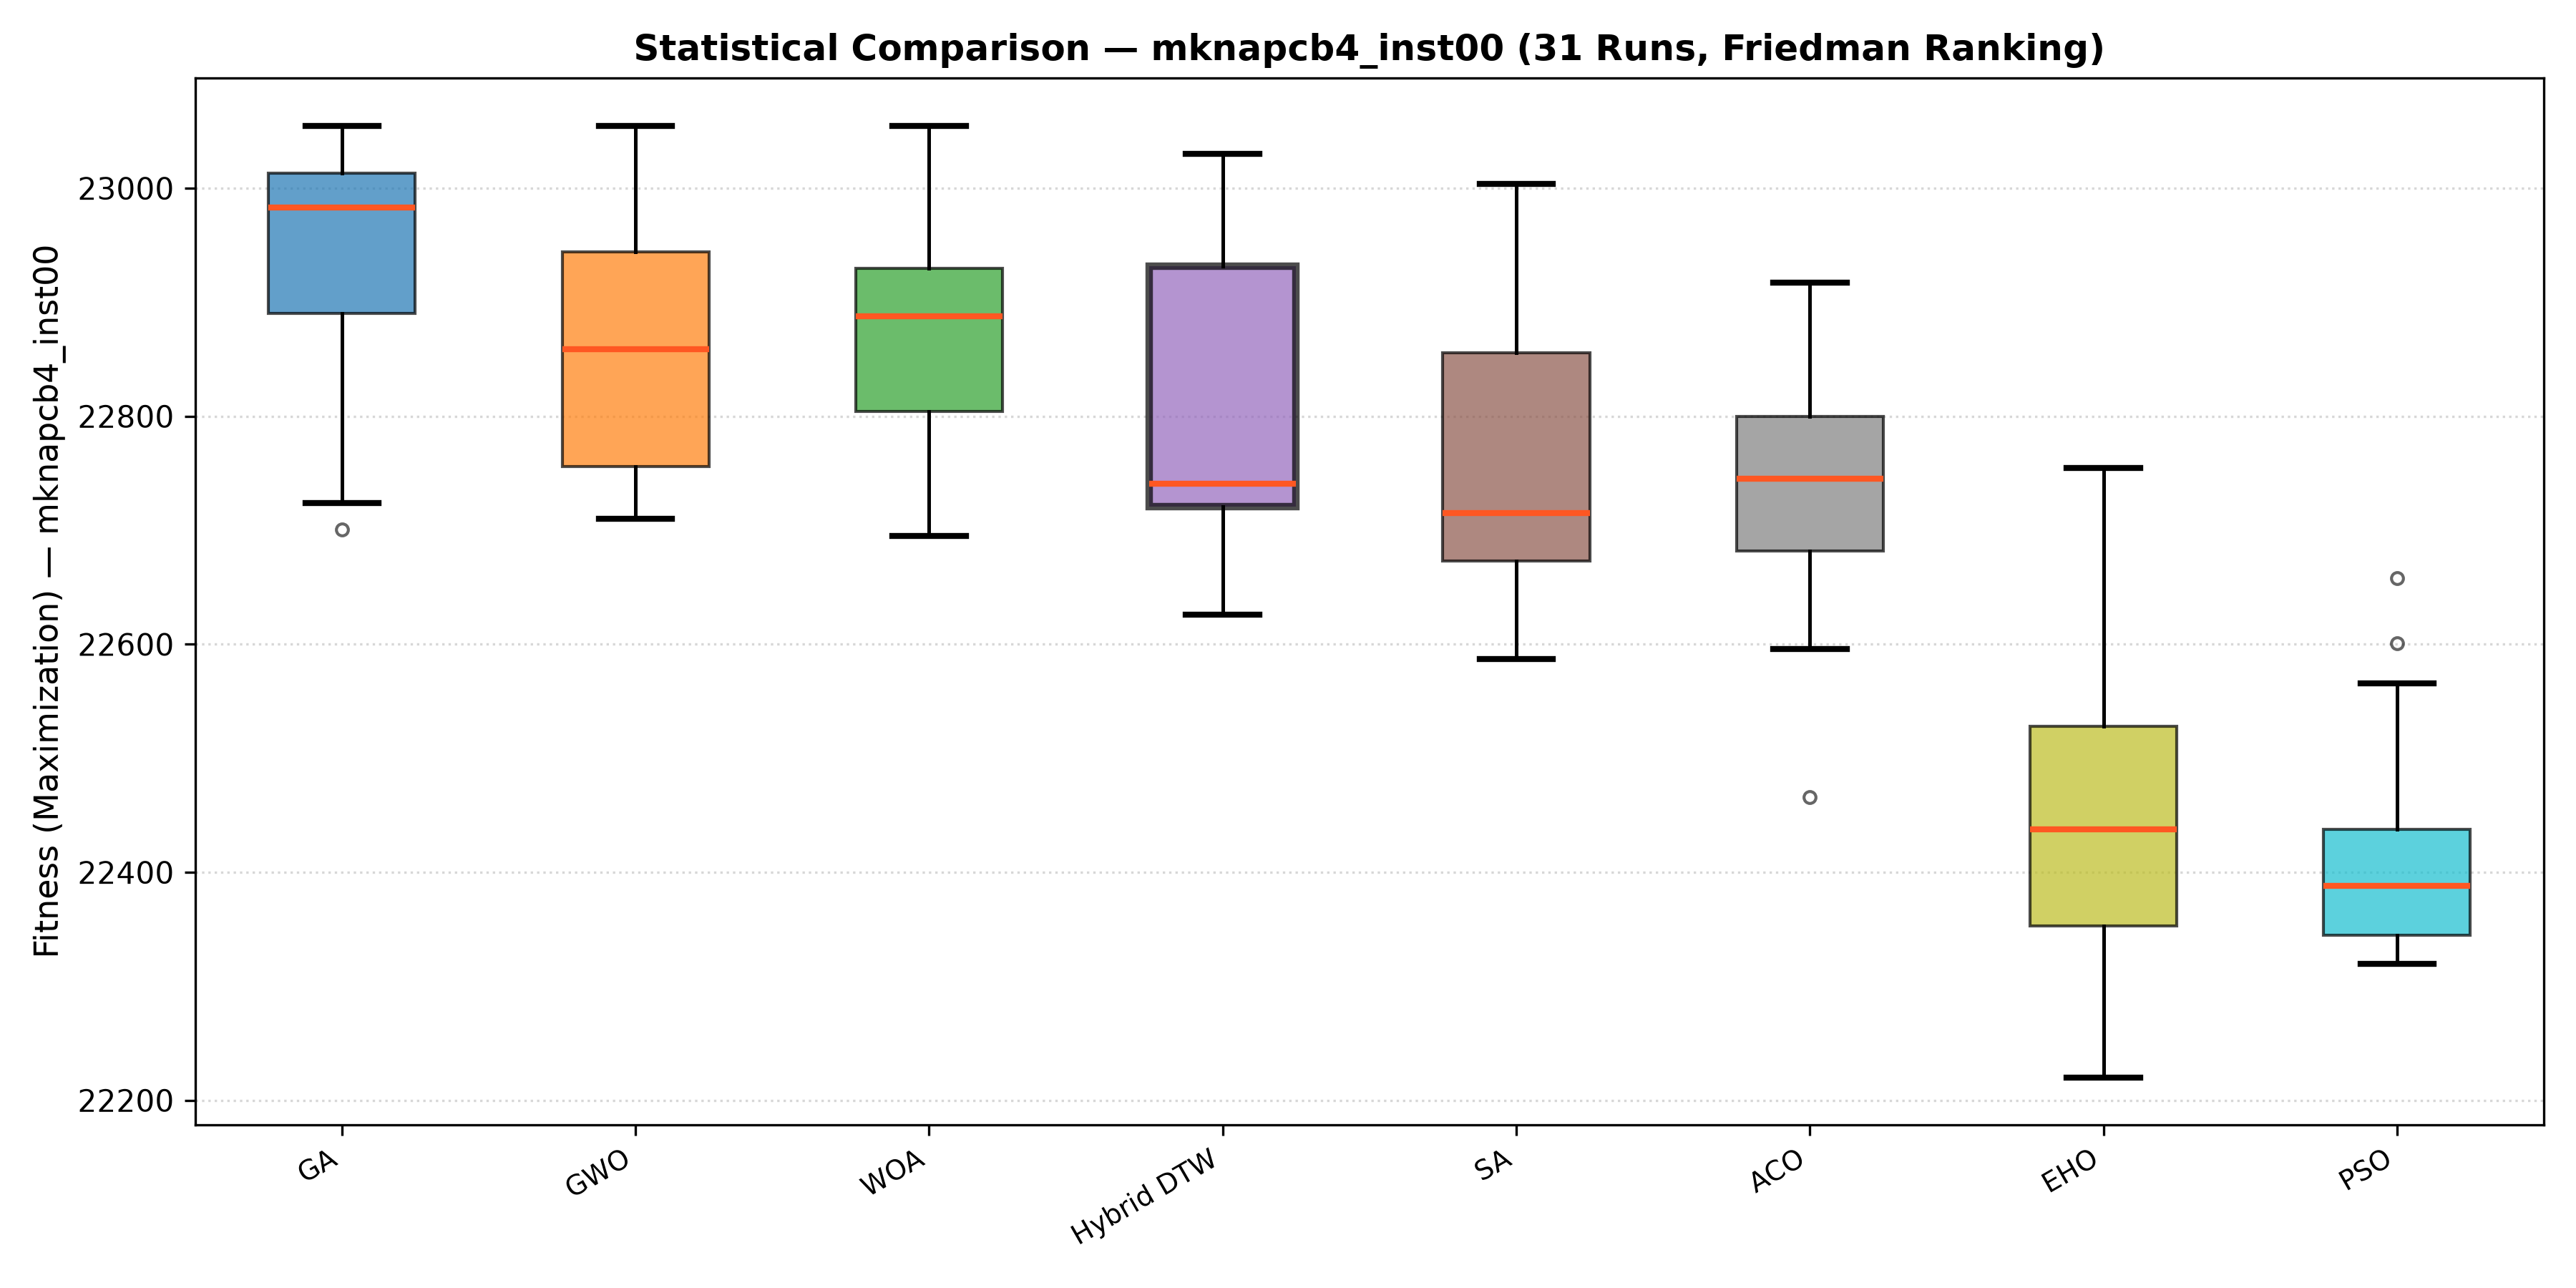
\includegraphics[width=0.32\textwidth]{imagenes_paper/mkp_dtw_3k_mknapcb4_comparativo_mh.png}}\hfill
\subfloat[Best-run convergence.]{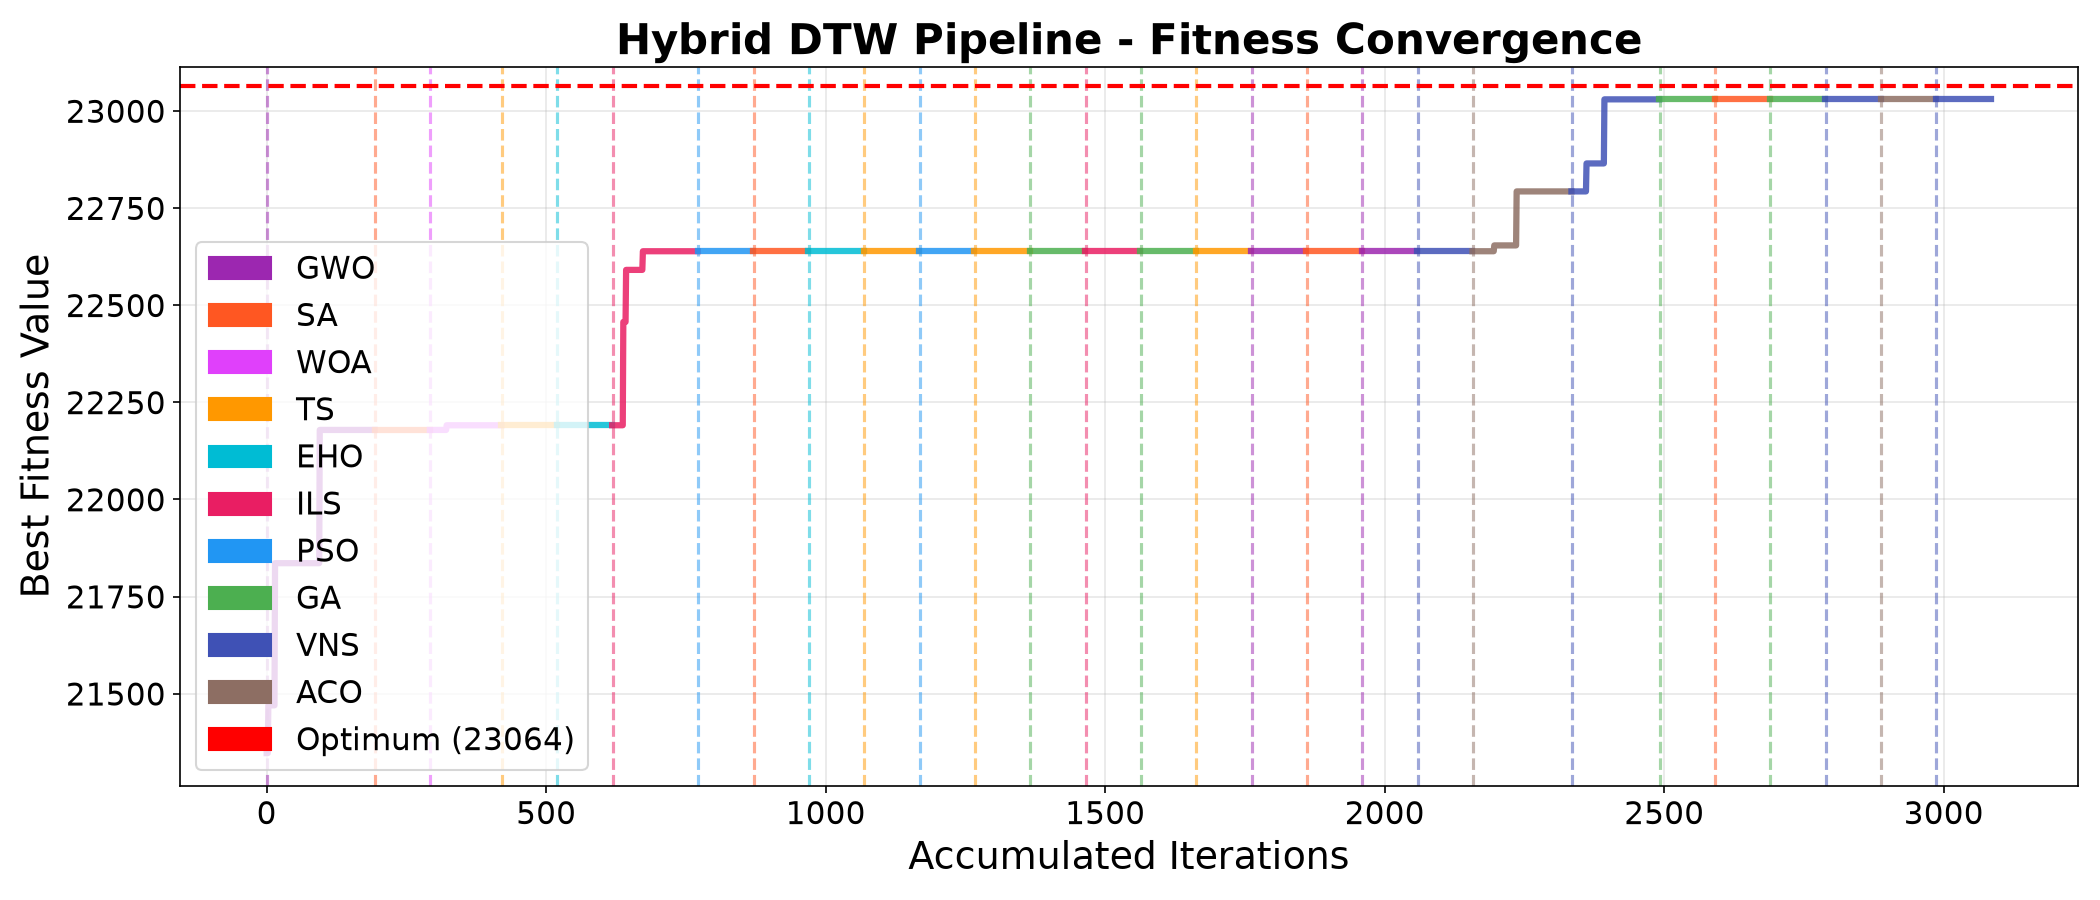
\includegraphics[width=0.32\textwidth]{imagenes_paper/mkp_dtw_3k_mknapcb4_convergencia.png}}\hfill
\subfloat[Elastic metric $\Delta=D_1-D_2$.]{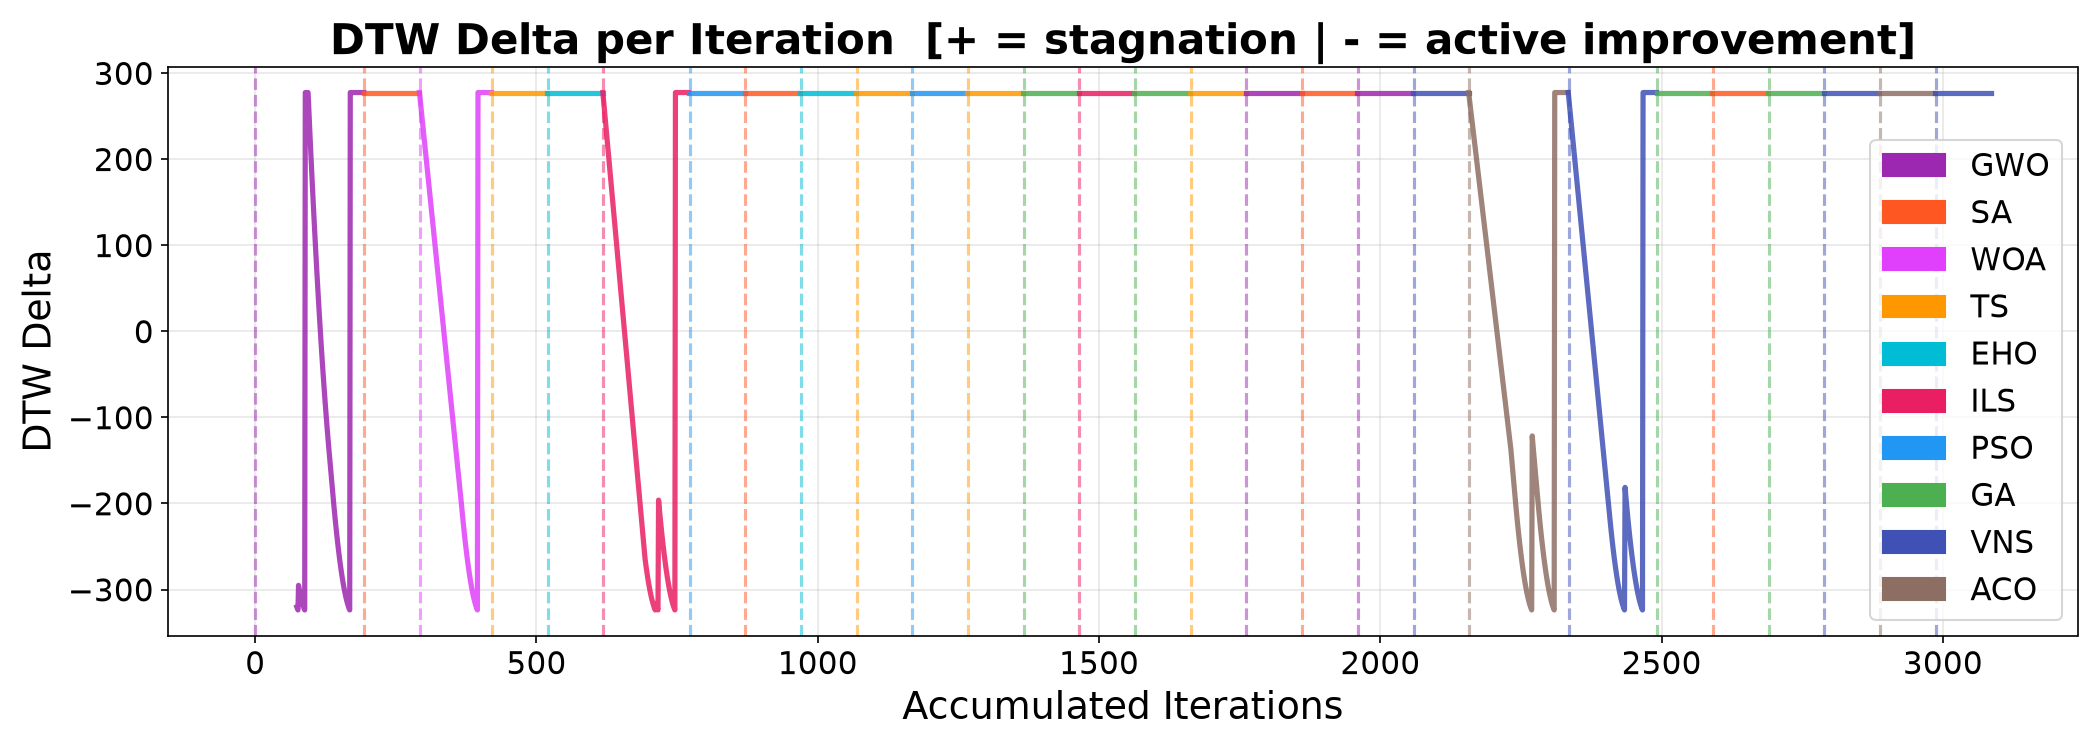
\includegraphics[width=0.32\textwidth]{imagenes_paper/mkp_dtw_3k_mknapcb4_delta.png}}
\caption{Diagnostic suite for instance \textbf{mknapcb4} ($n=100$, $m=10$) under the DTW framework with $T_{\max}=3{,}000$: (a)~final-fitness distribution over $N=31$ runs; (b)~convergence trajectory of the best run; (c)~elastic warping profile $\Delta$.}
\label{fig:mkp-best-cb4}
\end{figure}

% --- mknapcb5: DTW, 3,000 iterations ---
\begin{figure}[htbp]
\centering
\subfloat[Metaheuristic comparison.]{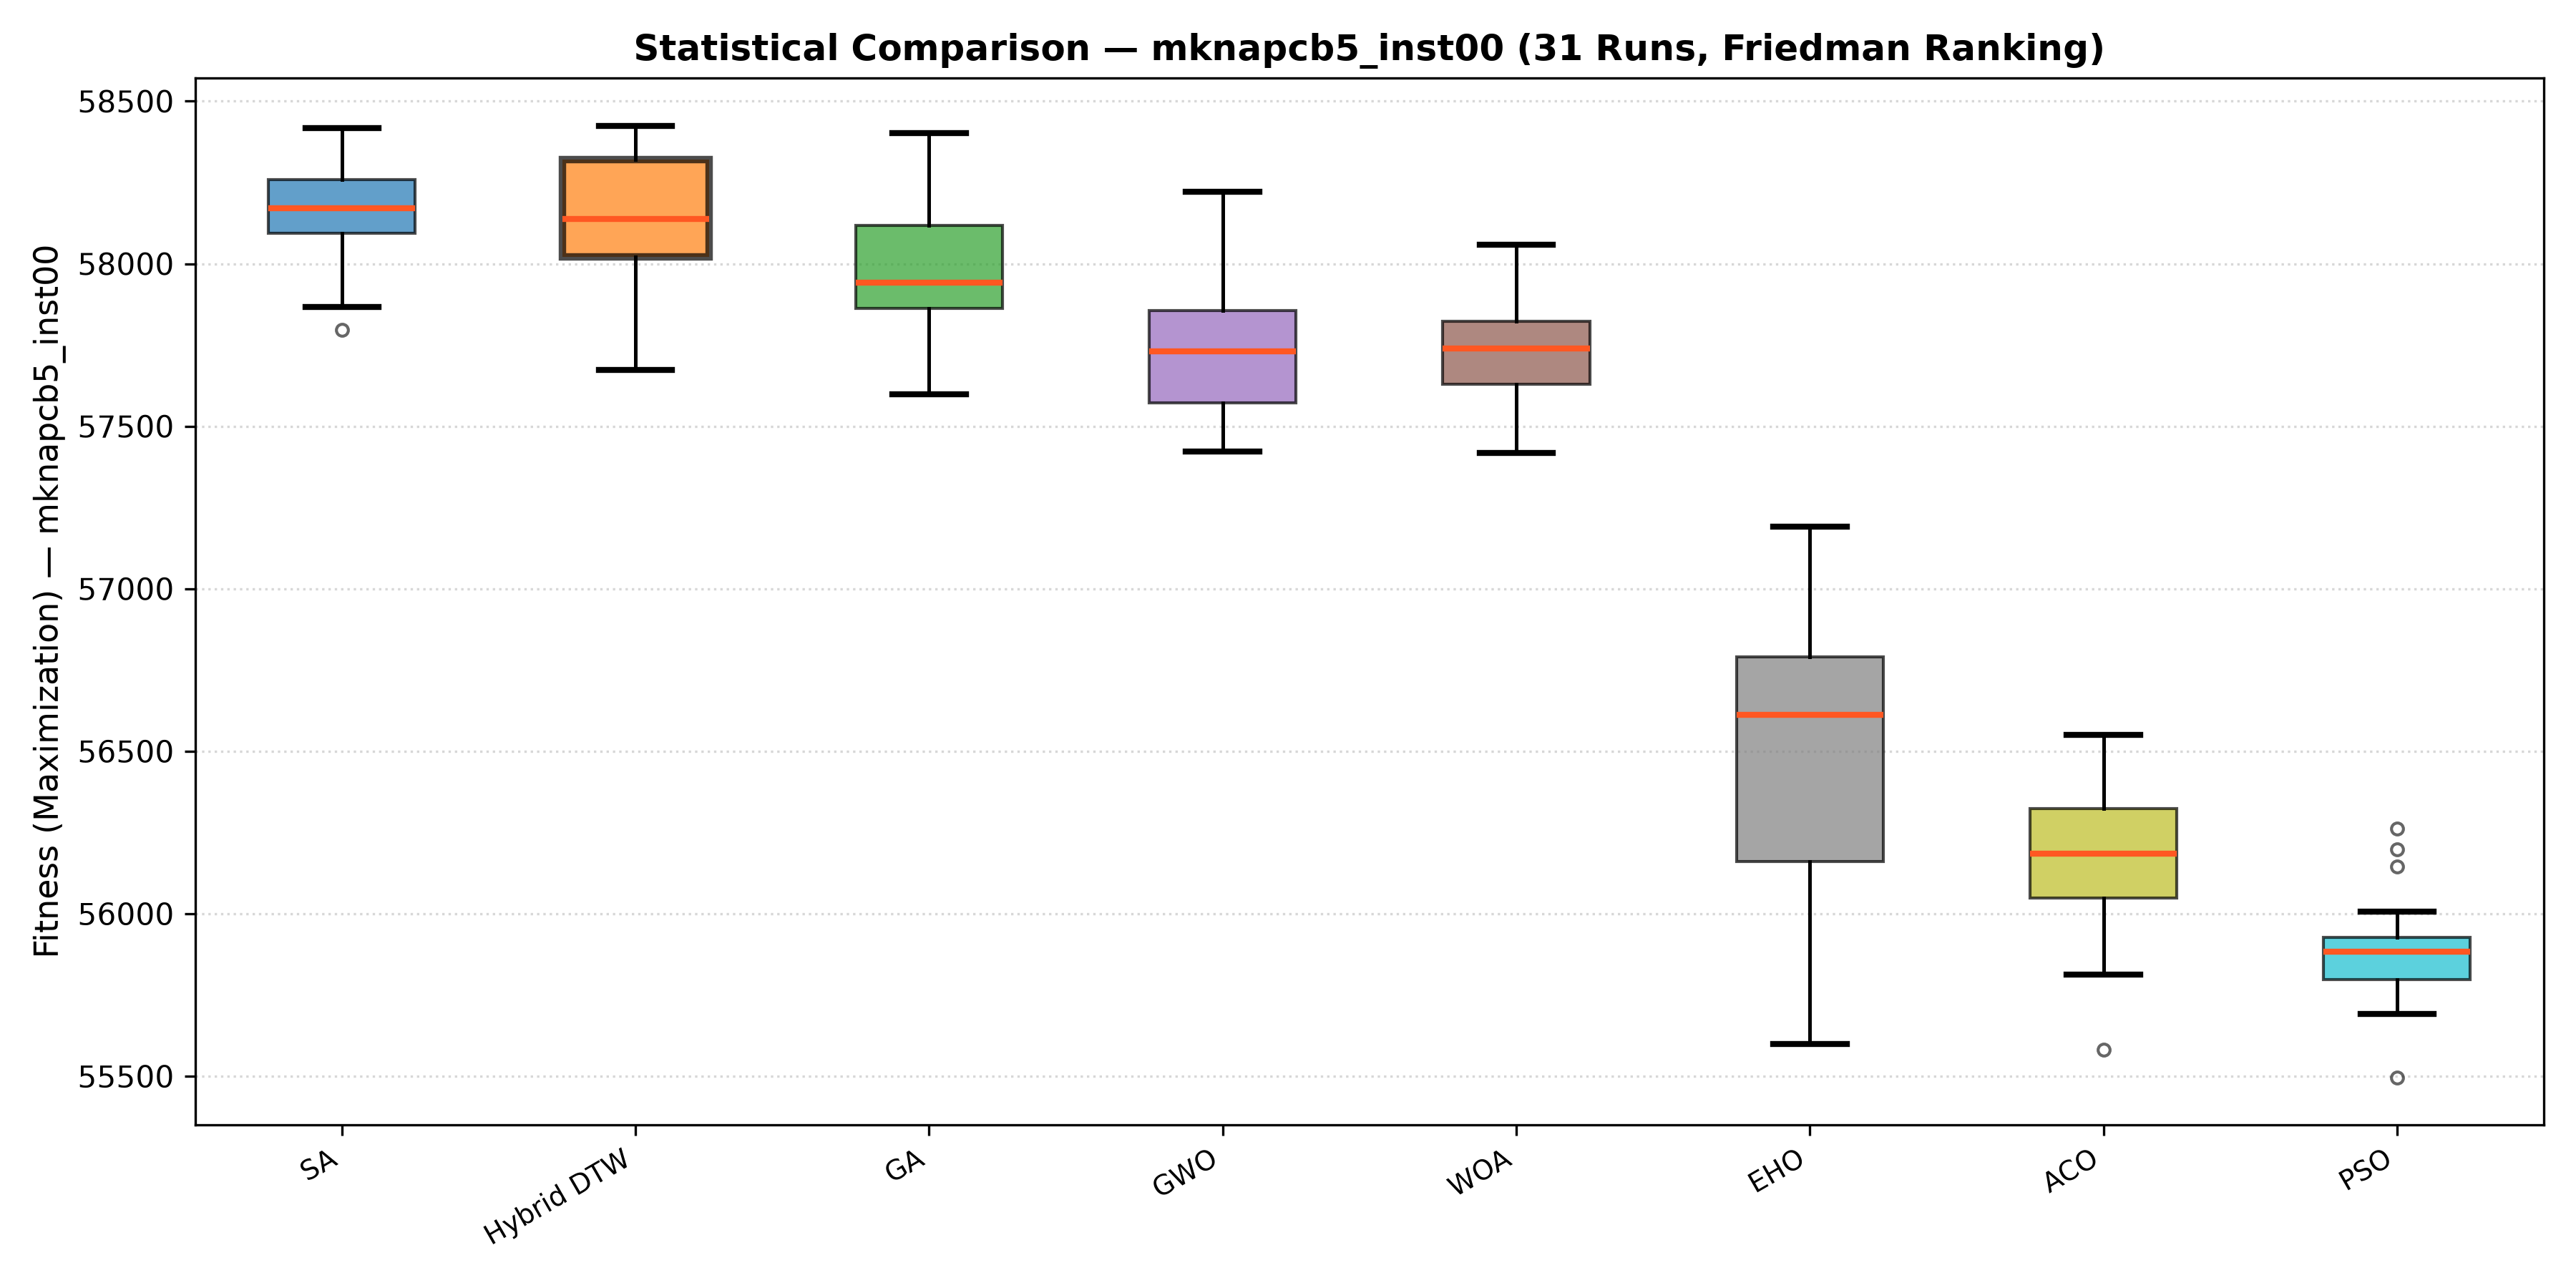
\includegraphics[width=0.32\textwidth]{imagenes_paper/mkp_dtw_3k_mknapcb5_comparativo_mh.png}}\hfill
\subfloat[Best-run convergence.]{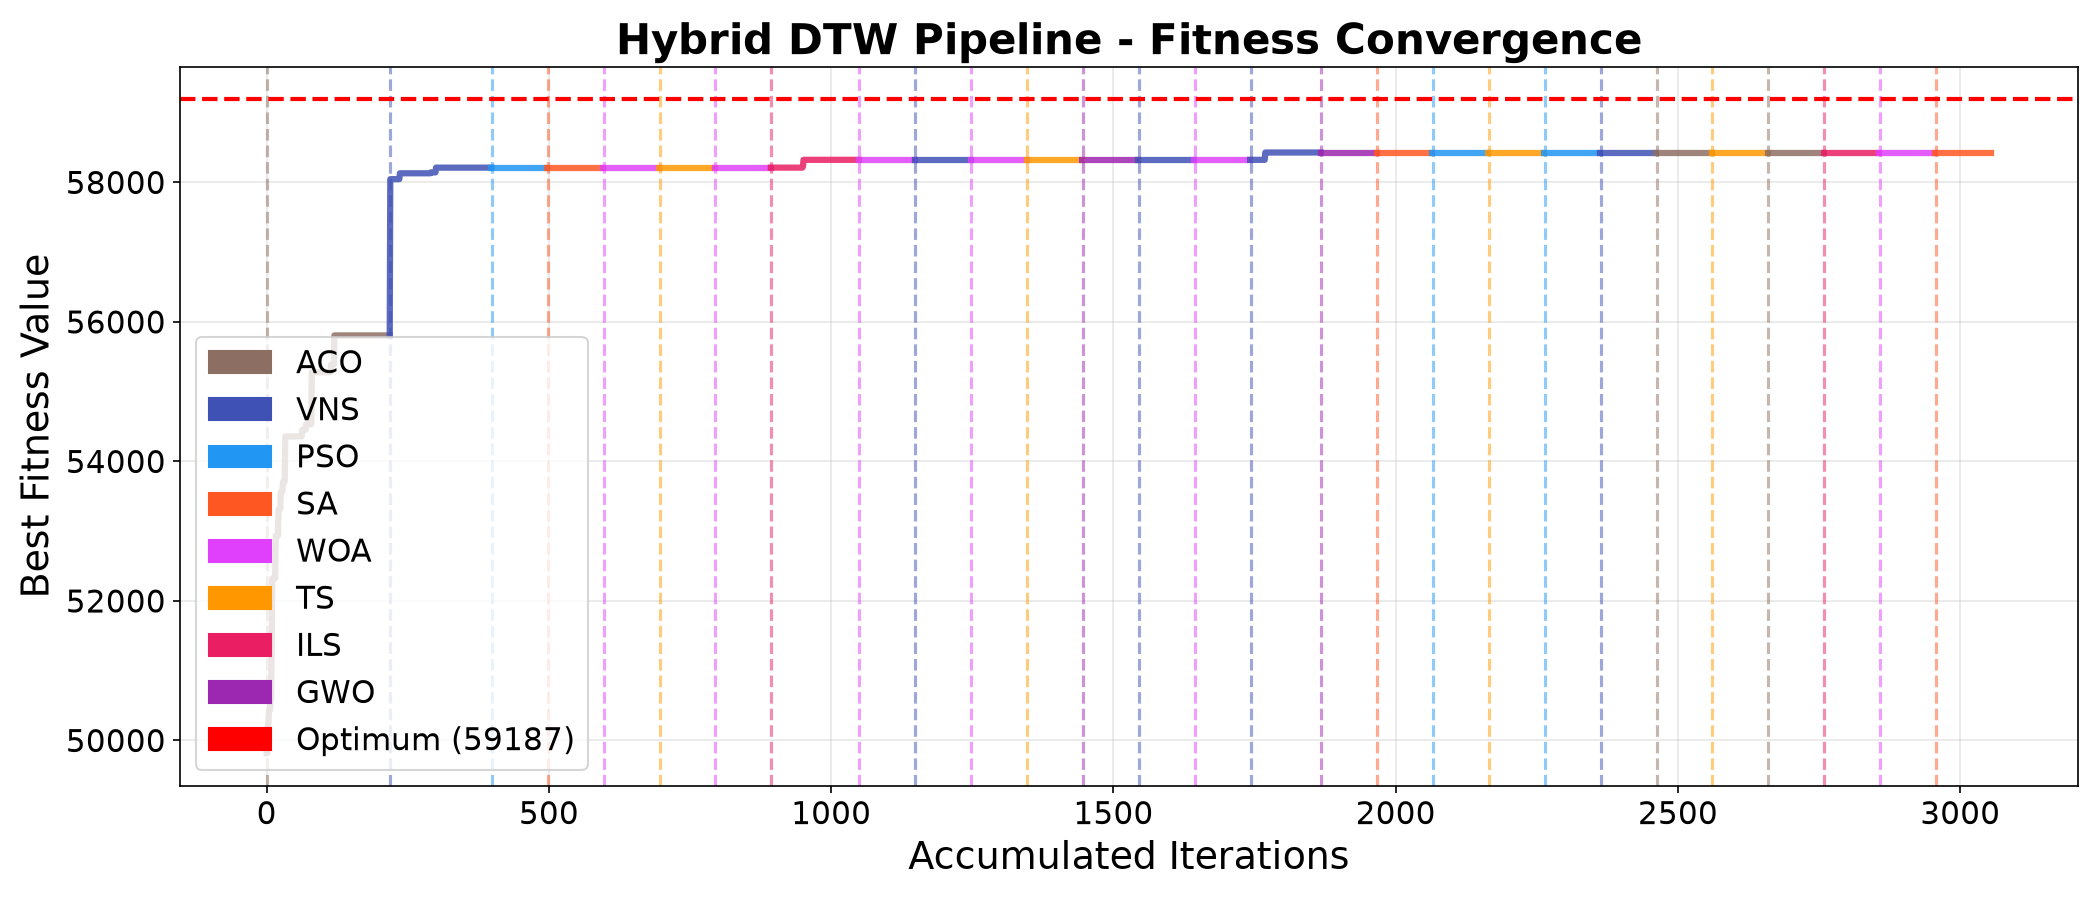
\includegraphics[width=0.32\textwidth]{imagenes_paper/mkp_dtw_3k_mknapcb5_convergencia.png}}\hfill
\subfloat[Elastic metric $\Delta=D_1-D_2$.]{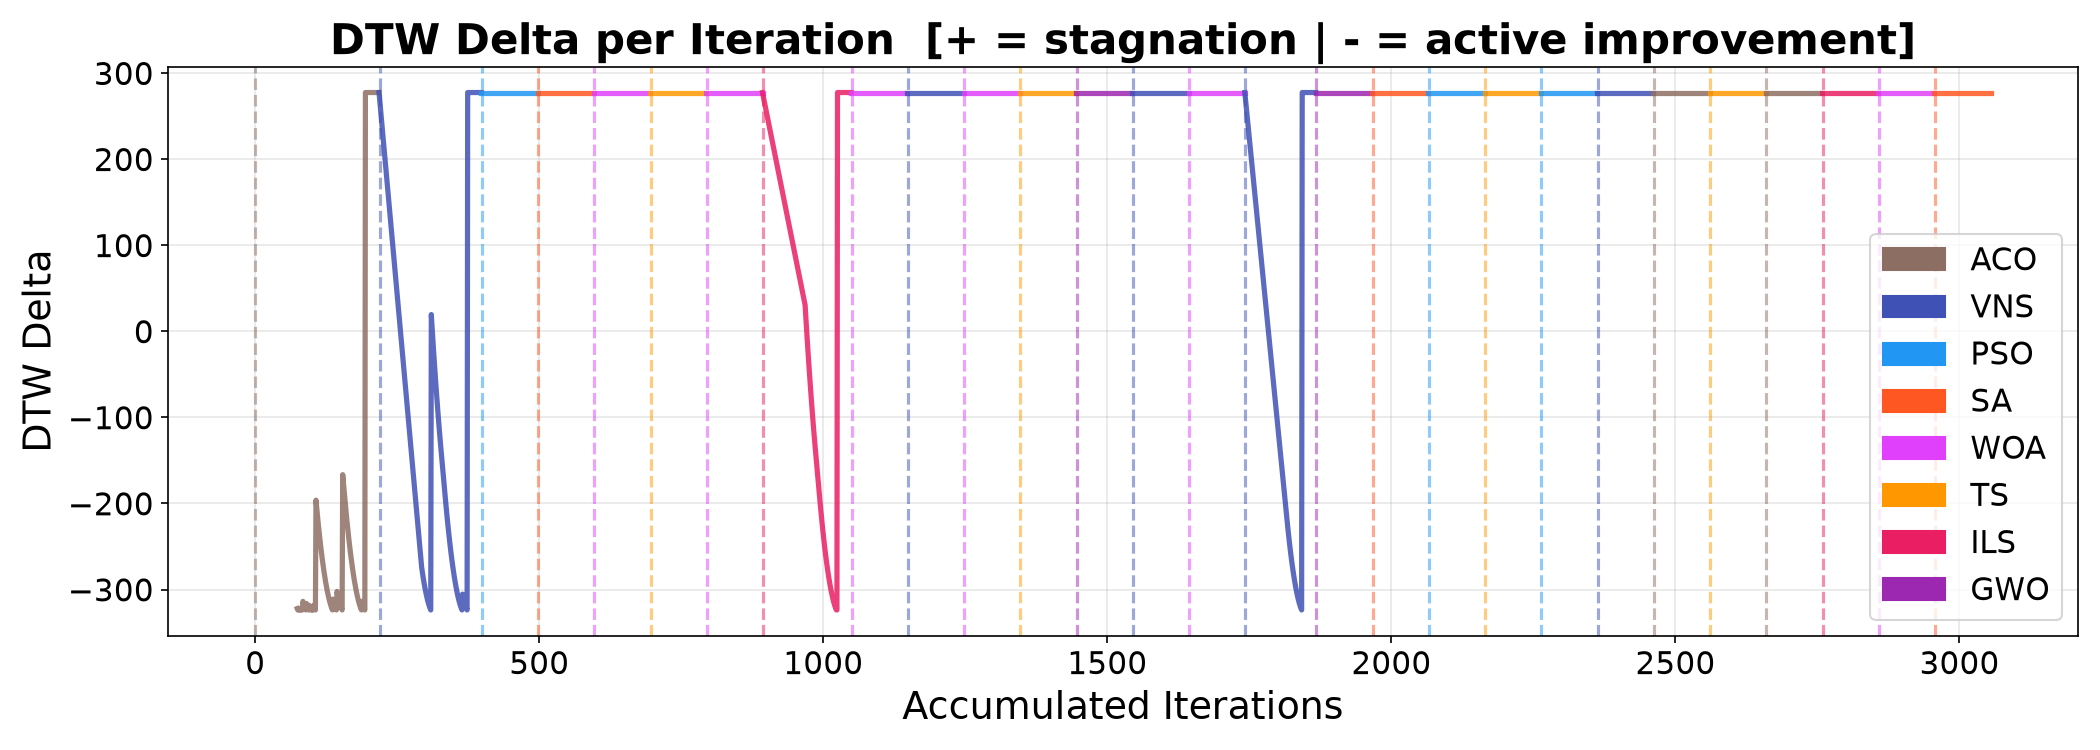
\includegraphics[width=0.32\textwidth]{imagenes_paper/mkp_dtw_3k_mknapcb5_delta.png}}
\caption{Diagnostic suite for instance \textbf{mknapcb5} ($n=250$, $m=10$) under the DTW framework with $T_{\max}=3{,}000$: (a)~final-fitness distribution over $N=31$ runs; (b)~convergence trajectory of the best run; (c)~elastic warping profile $\Delta$.}
\label{fig:mkp-best-cb5}
\end{figure}

% --- mknapcb6: DTW, 3,000 iterations ---
\begin{figure}[htbp]
\centering
\subfloat[Metaheuristic comparison.]{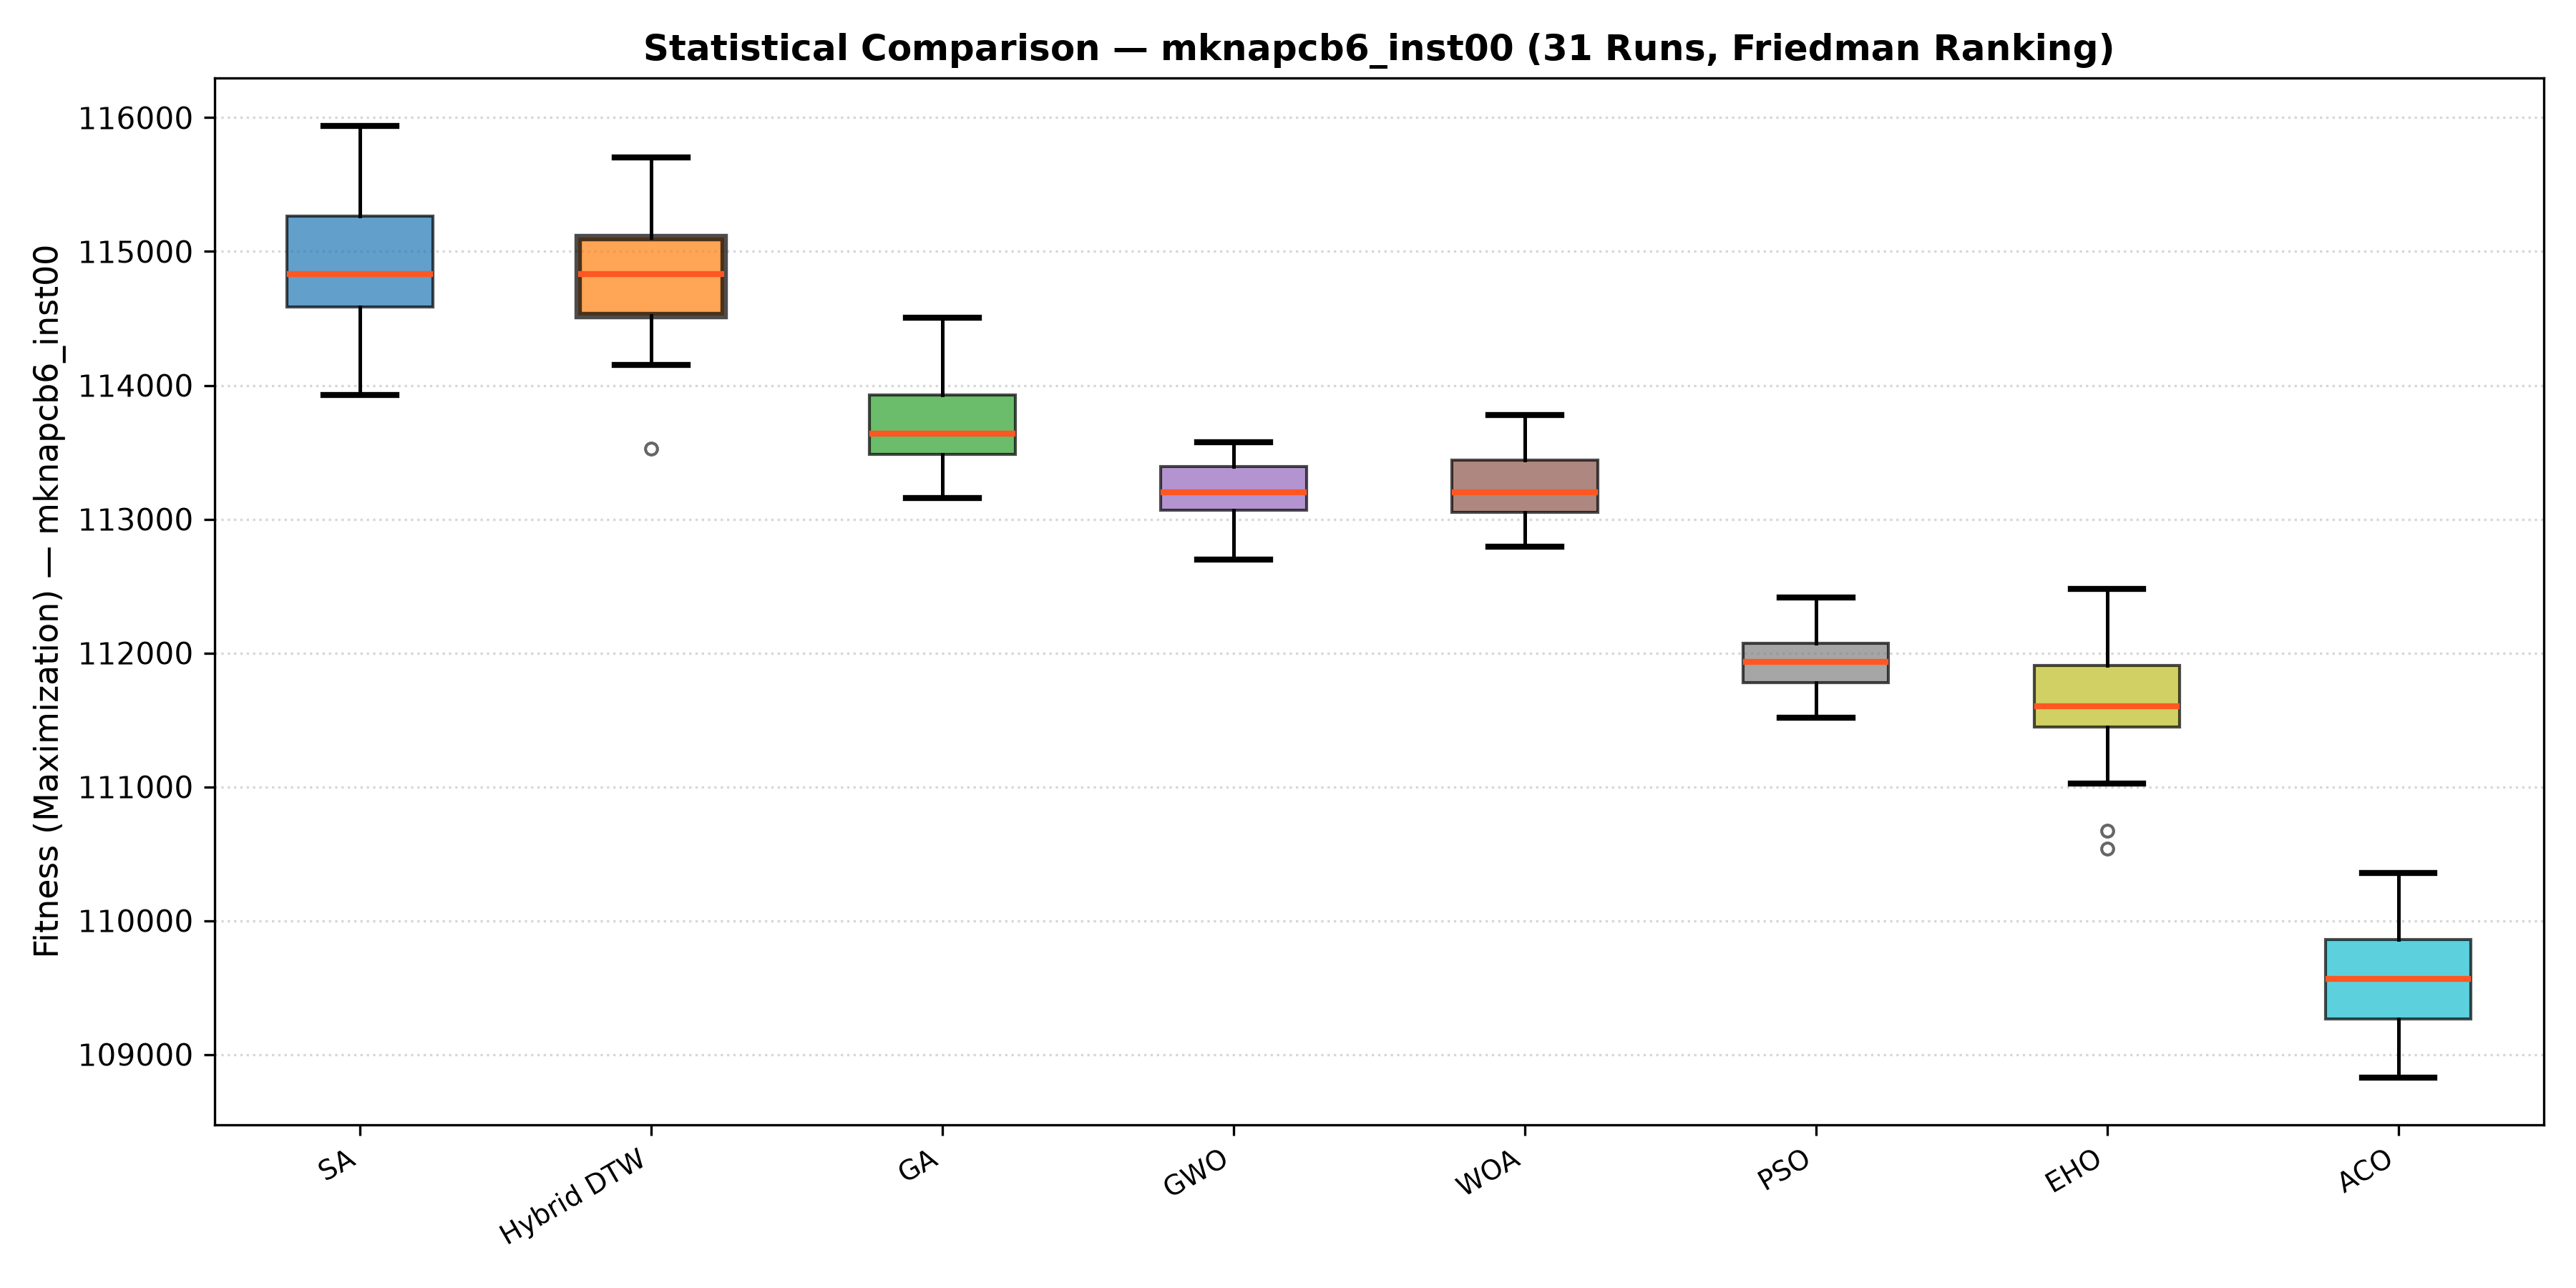
\includegraphics[width=0.32\textwidth]{imagenes_paper/mkp_dtw_3k_mknapcb6_comparativo_mh.png}}\hfill
\subfloat[Best-run convergence.]{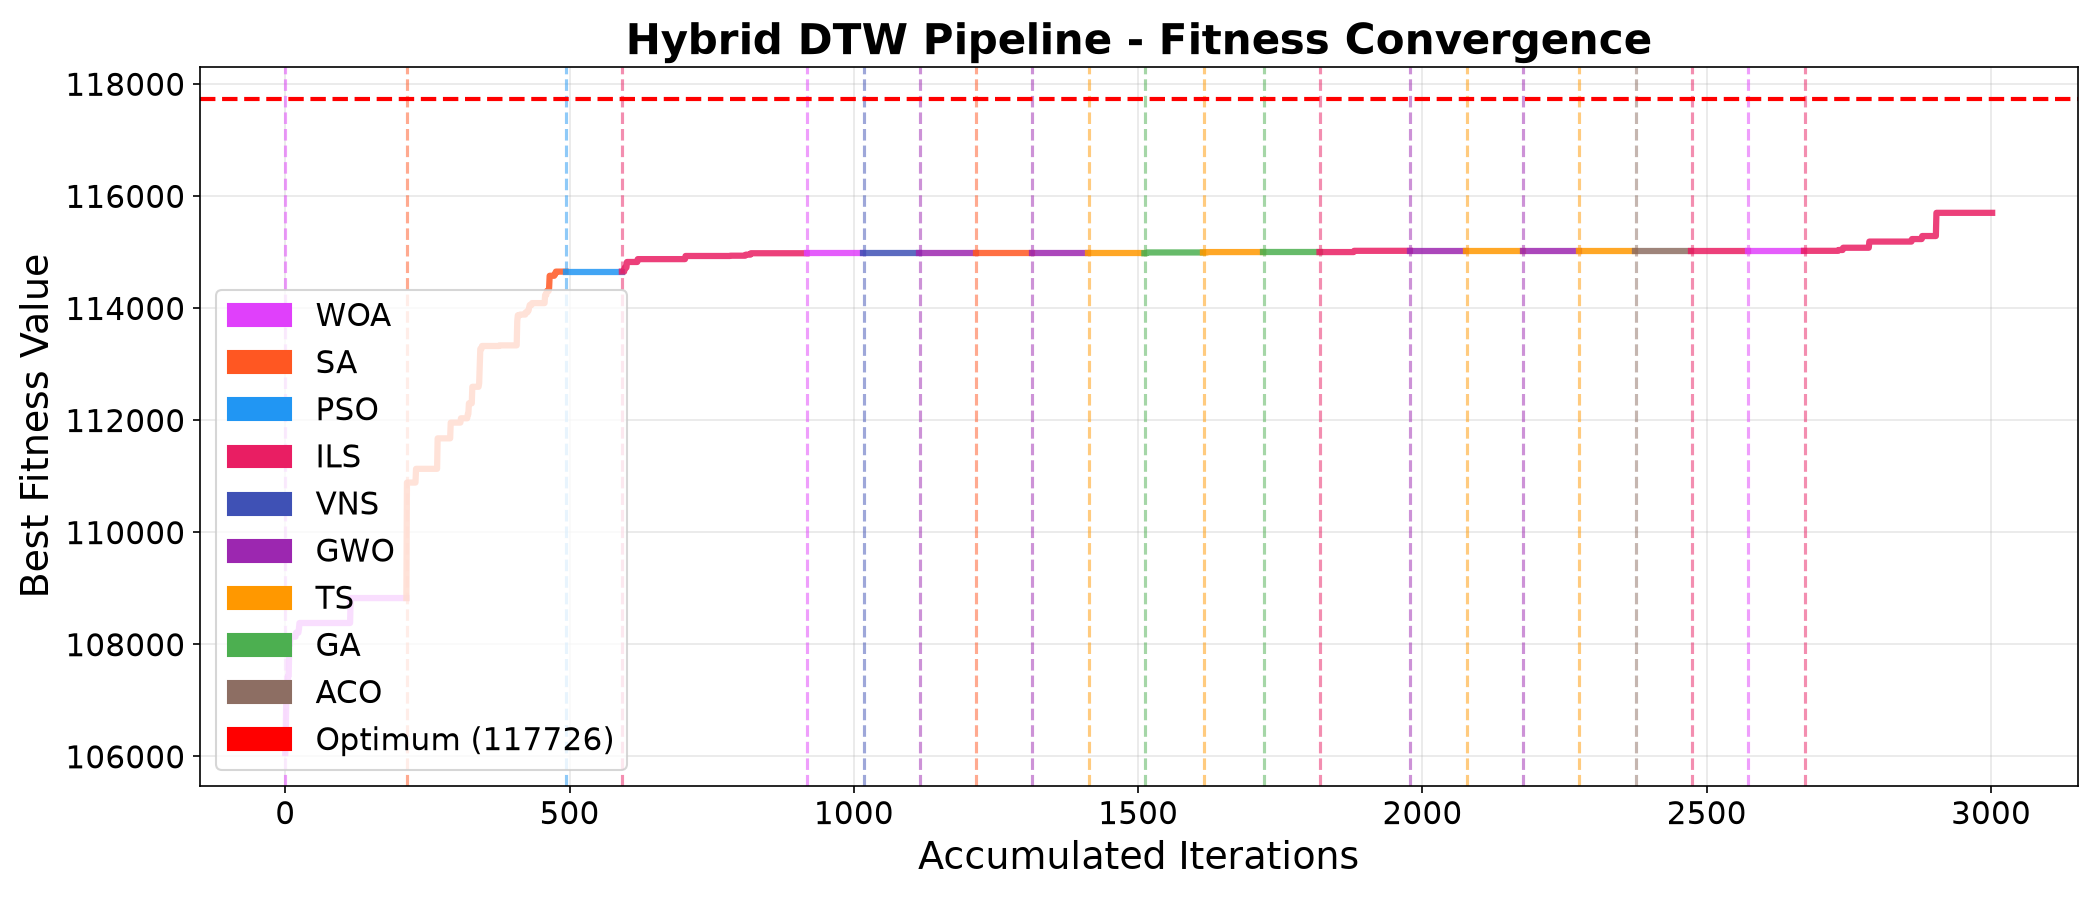
\includegraphics[width=0.32\textwidth]{imagenes_paper/mkp_dtw_3k_mknapcb6_convergencia.png}}\hfill
\subfloat[Elastic metric $\Delta=D_1-D_2$.]{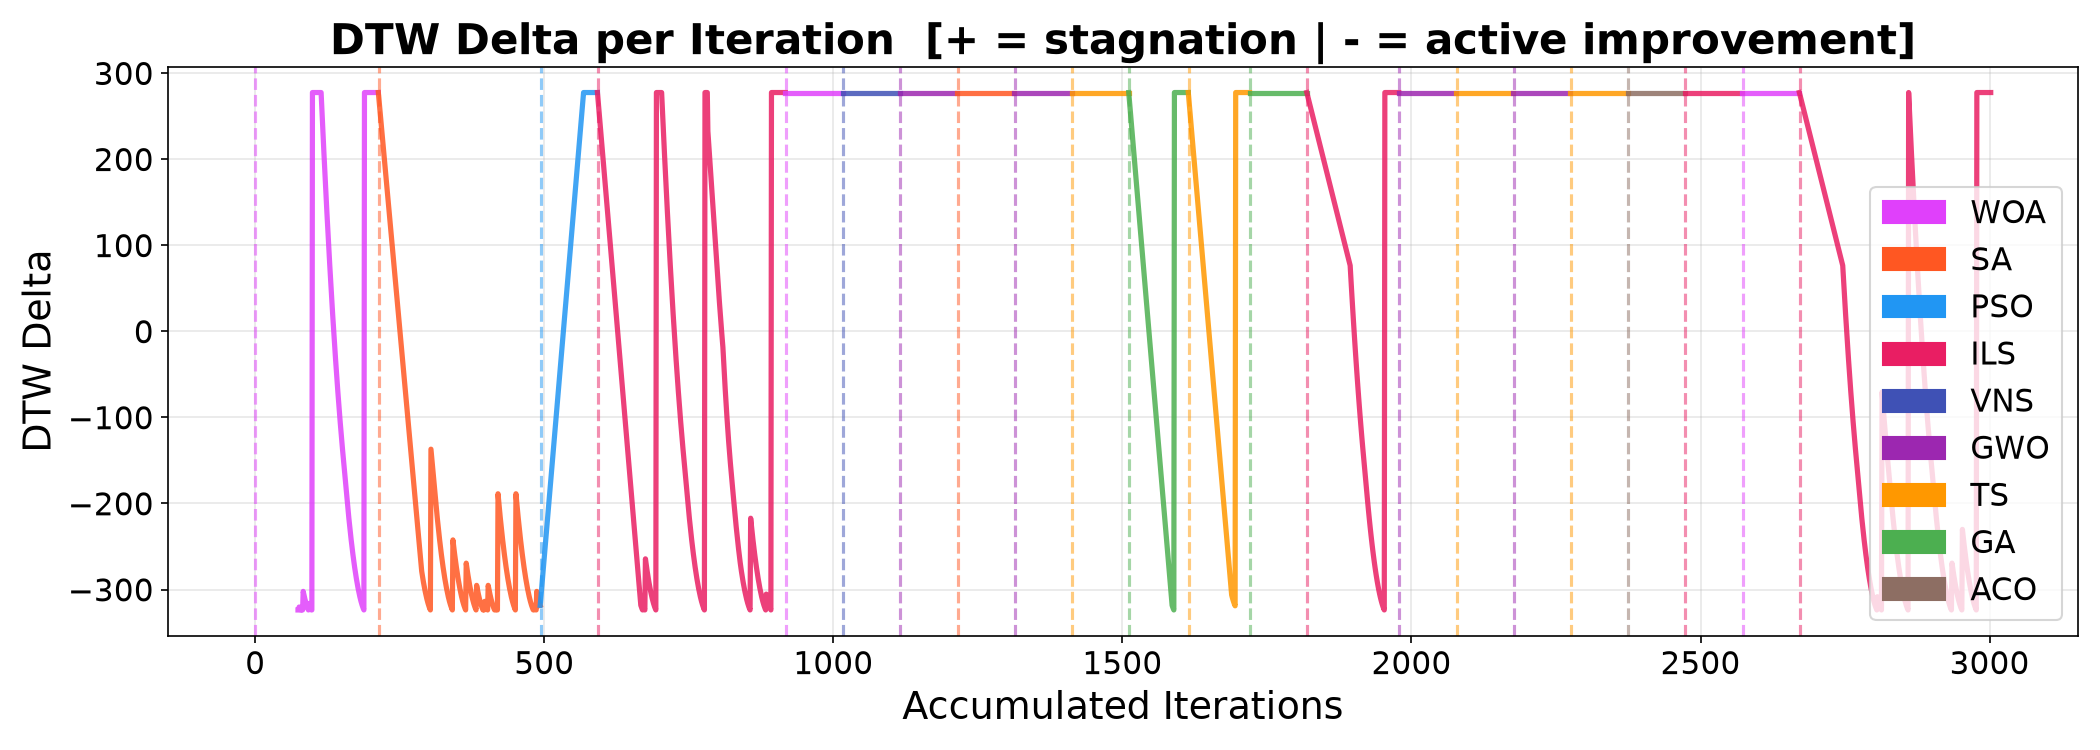
\includegraphics[width=0.32\textwidth]{imagenes_paper/mkp_dtw_3k_mknapcb6_delta.png}}
\caption{Diagnostic suite for instance \textbf{mknapcb6} ($n=500$, $m=10$) under the DTW framework with $T_{\max}=3{,}000$: (a)~final-fitness distribution over $N=31$ runs; (b)~convergence trajectory of the best run; (c)~elastic warping profile $\Delta$.}
\label{fig:mkp-best-cb6}
\end{figure}

% --- mknapcb7: DTW, 3,000 iterations ---
\begin{figure}[htbp]
\centering
\subfloat[Metaheuristic comparison.]{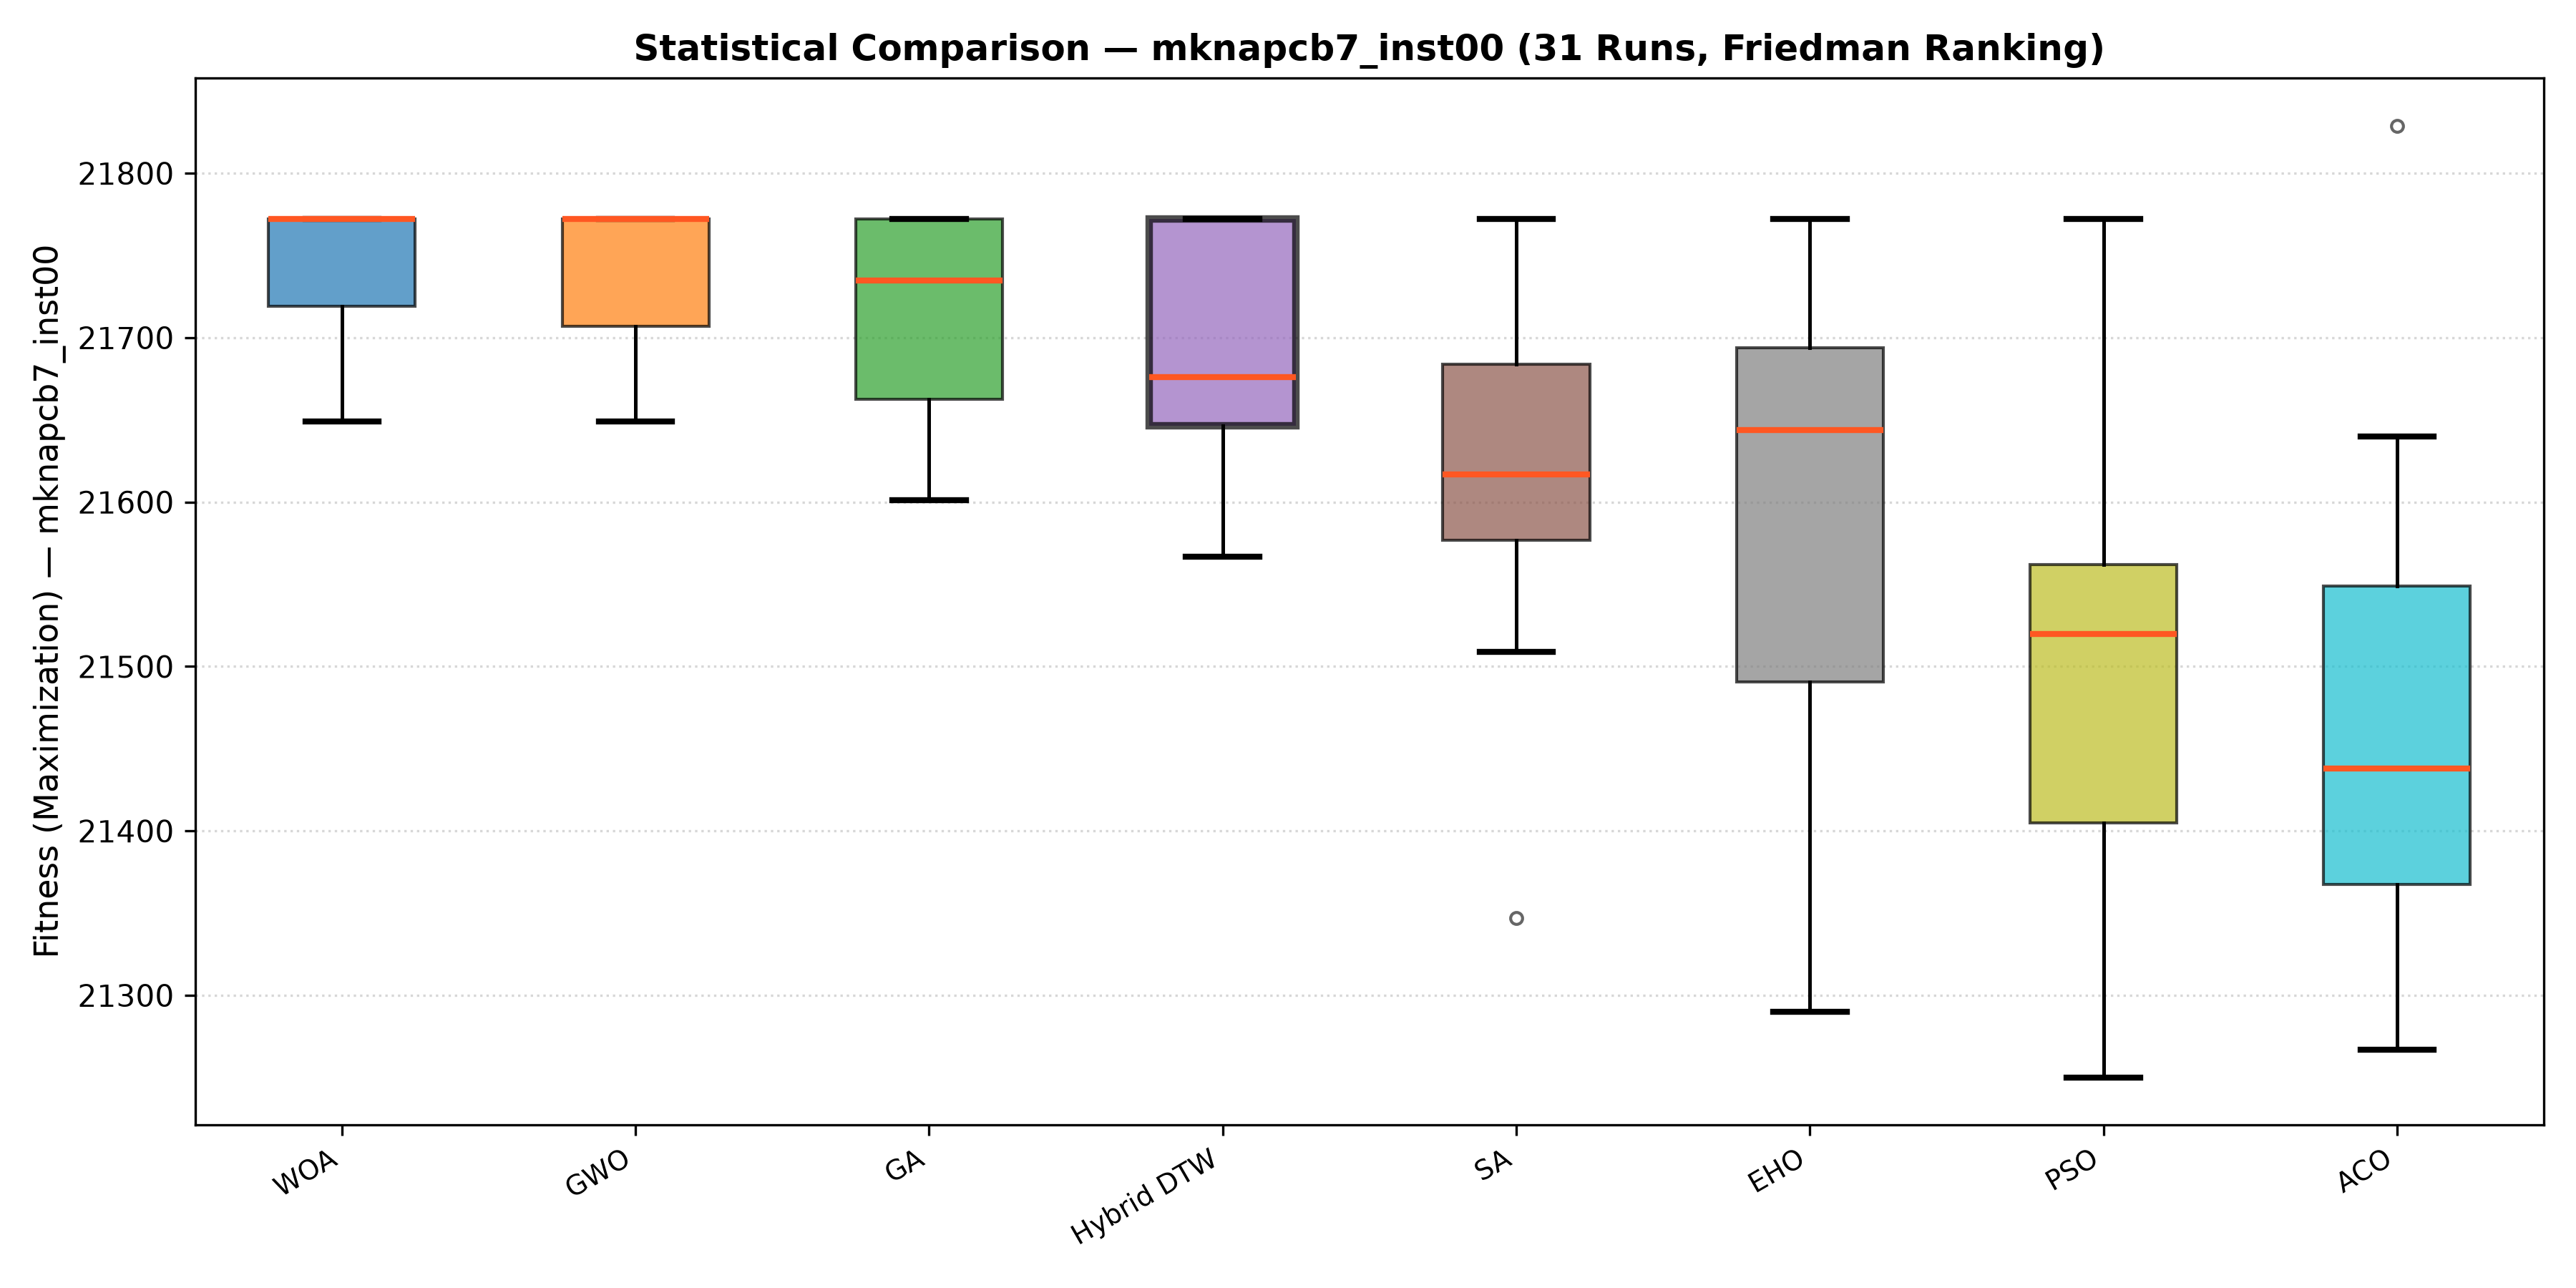
\includegraphics[width=0.32\textwidth]{imagenes_paper/mkp_dtw_3k_mknapcb7_comparativo_mh.png}}\hfill
\subfloat[Best-run convergence.]{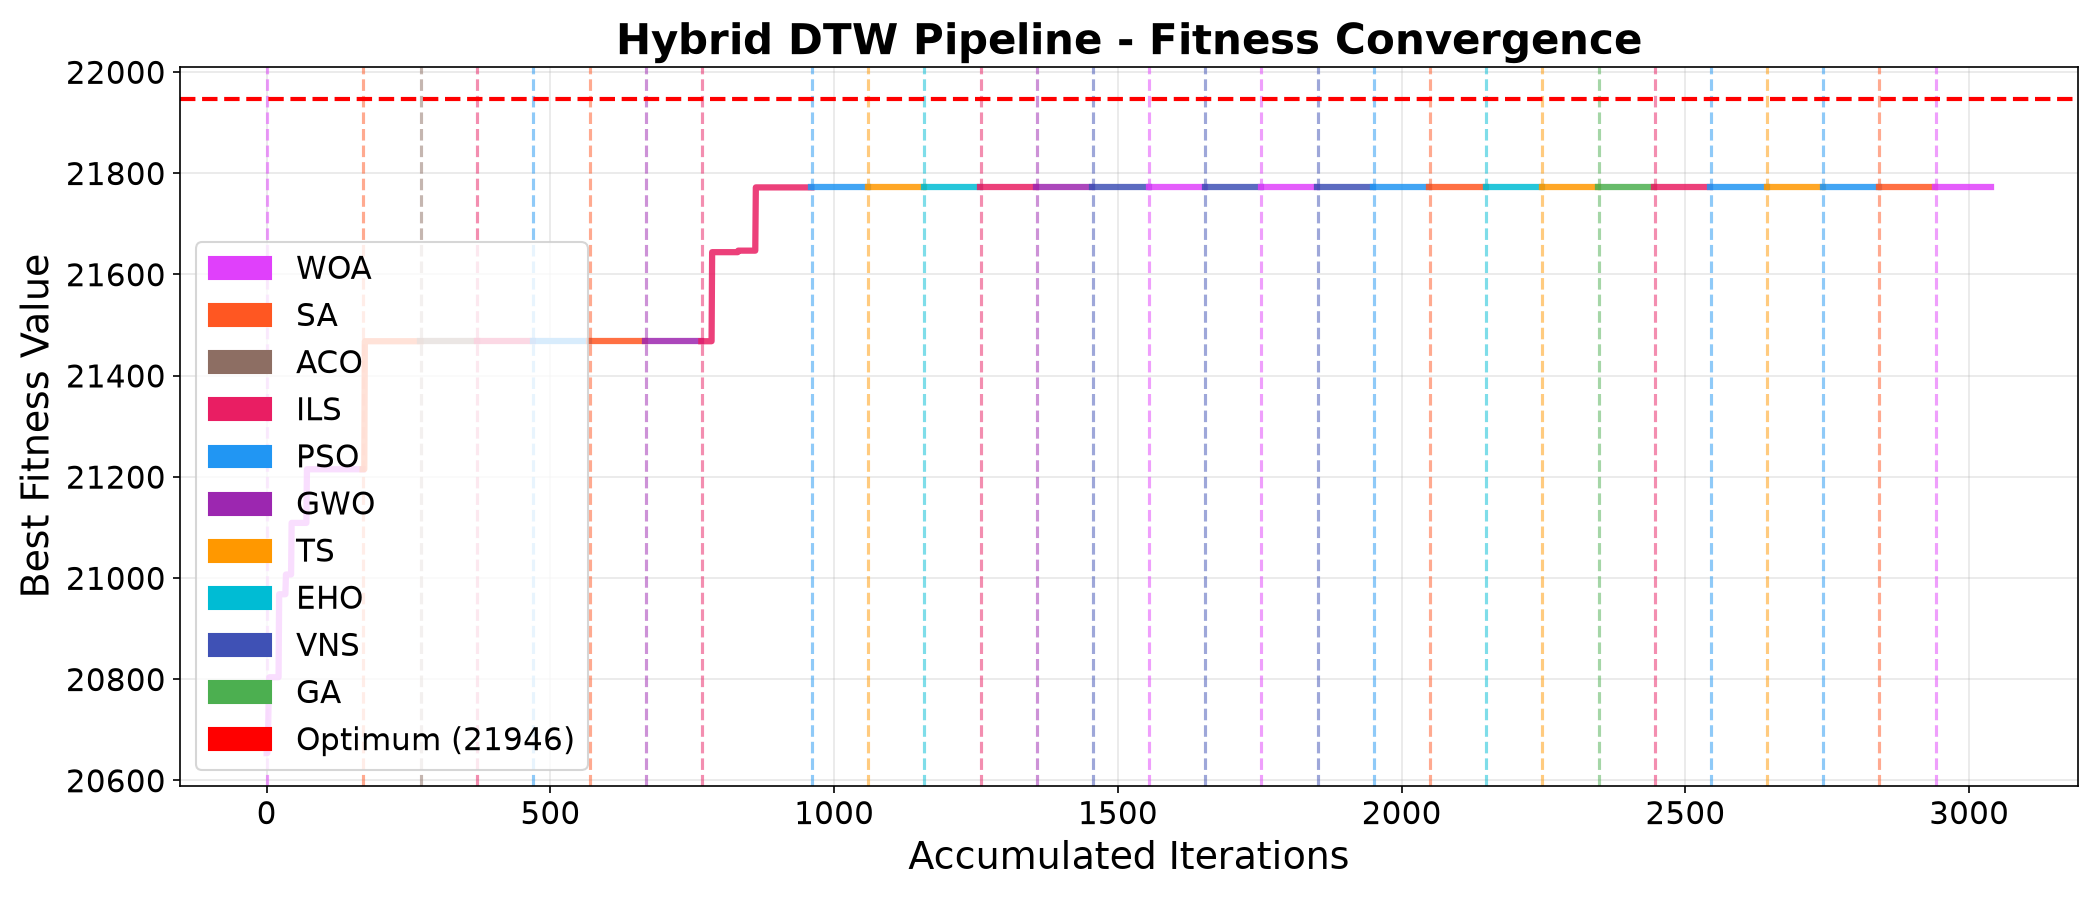
\includegraphics[width=0.32\textwidth]{imagenes_paper/mkp_dtw_3k_mknapcb7_convergencia.png}}\hfill
\subfloat[Elastic metric $\Delta=D_1-D_2$.]{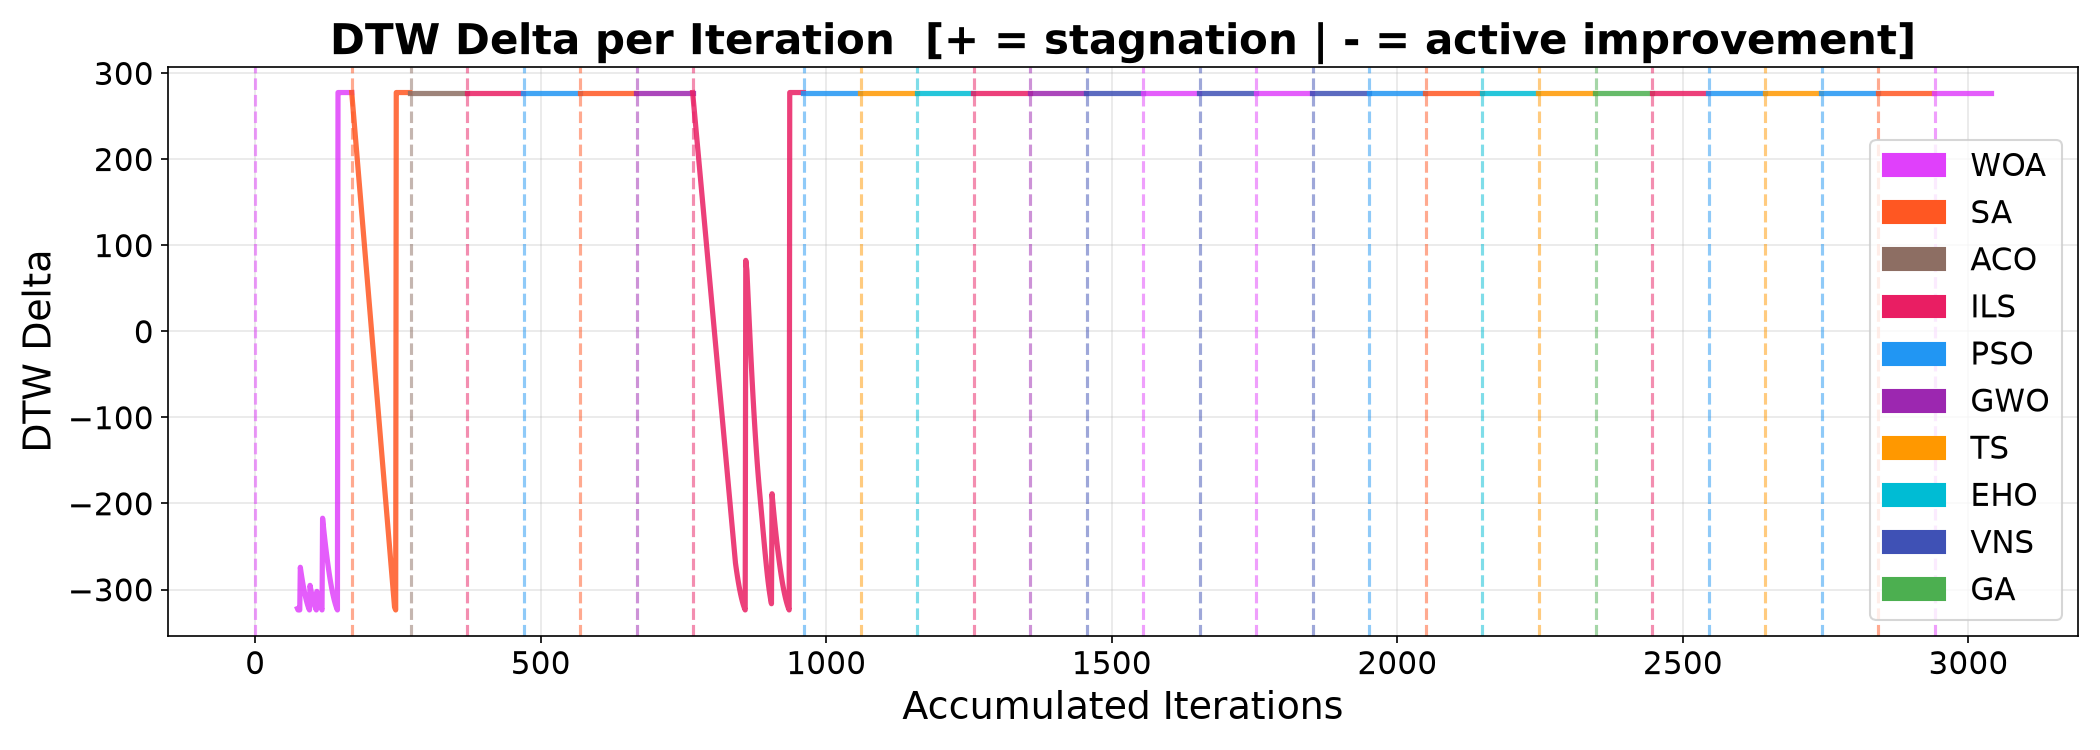
\includegraphics[width=0.32\textwidth]{imagenes_paper/mkp_dtw_3k_mknapcb7_delta.png}}
\caption{Diagnostic suite for instance \textbf{mknapcb7} ($n=100$, $m=30$) under the DTW framework with $T_{\max}=3{,}000$: (a)~final-fitness distribution over $N=31$ runs; (b)~convergence trajectory of the best run; (c)~elastic warping profile $\Delta$.}
\label{fig:mkp-best-cb7}
\end{figure}

% --- mknapcb8: DTW, 3,000 iterations ---
\begin{figure}[htbp]
\centering
\subfloat[Metaheuristic comparison.]{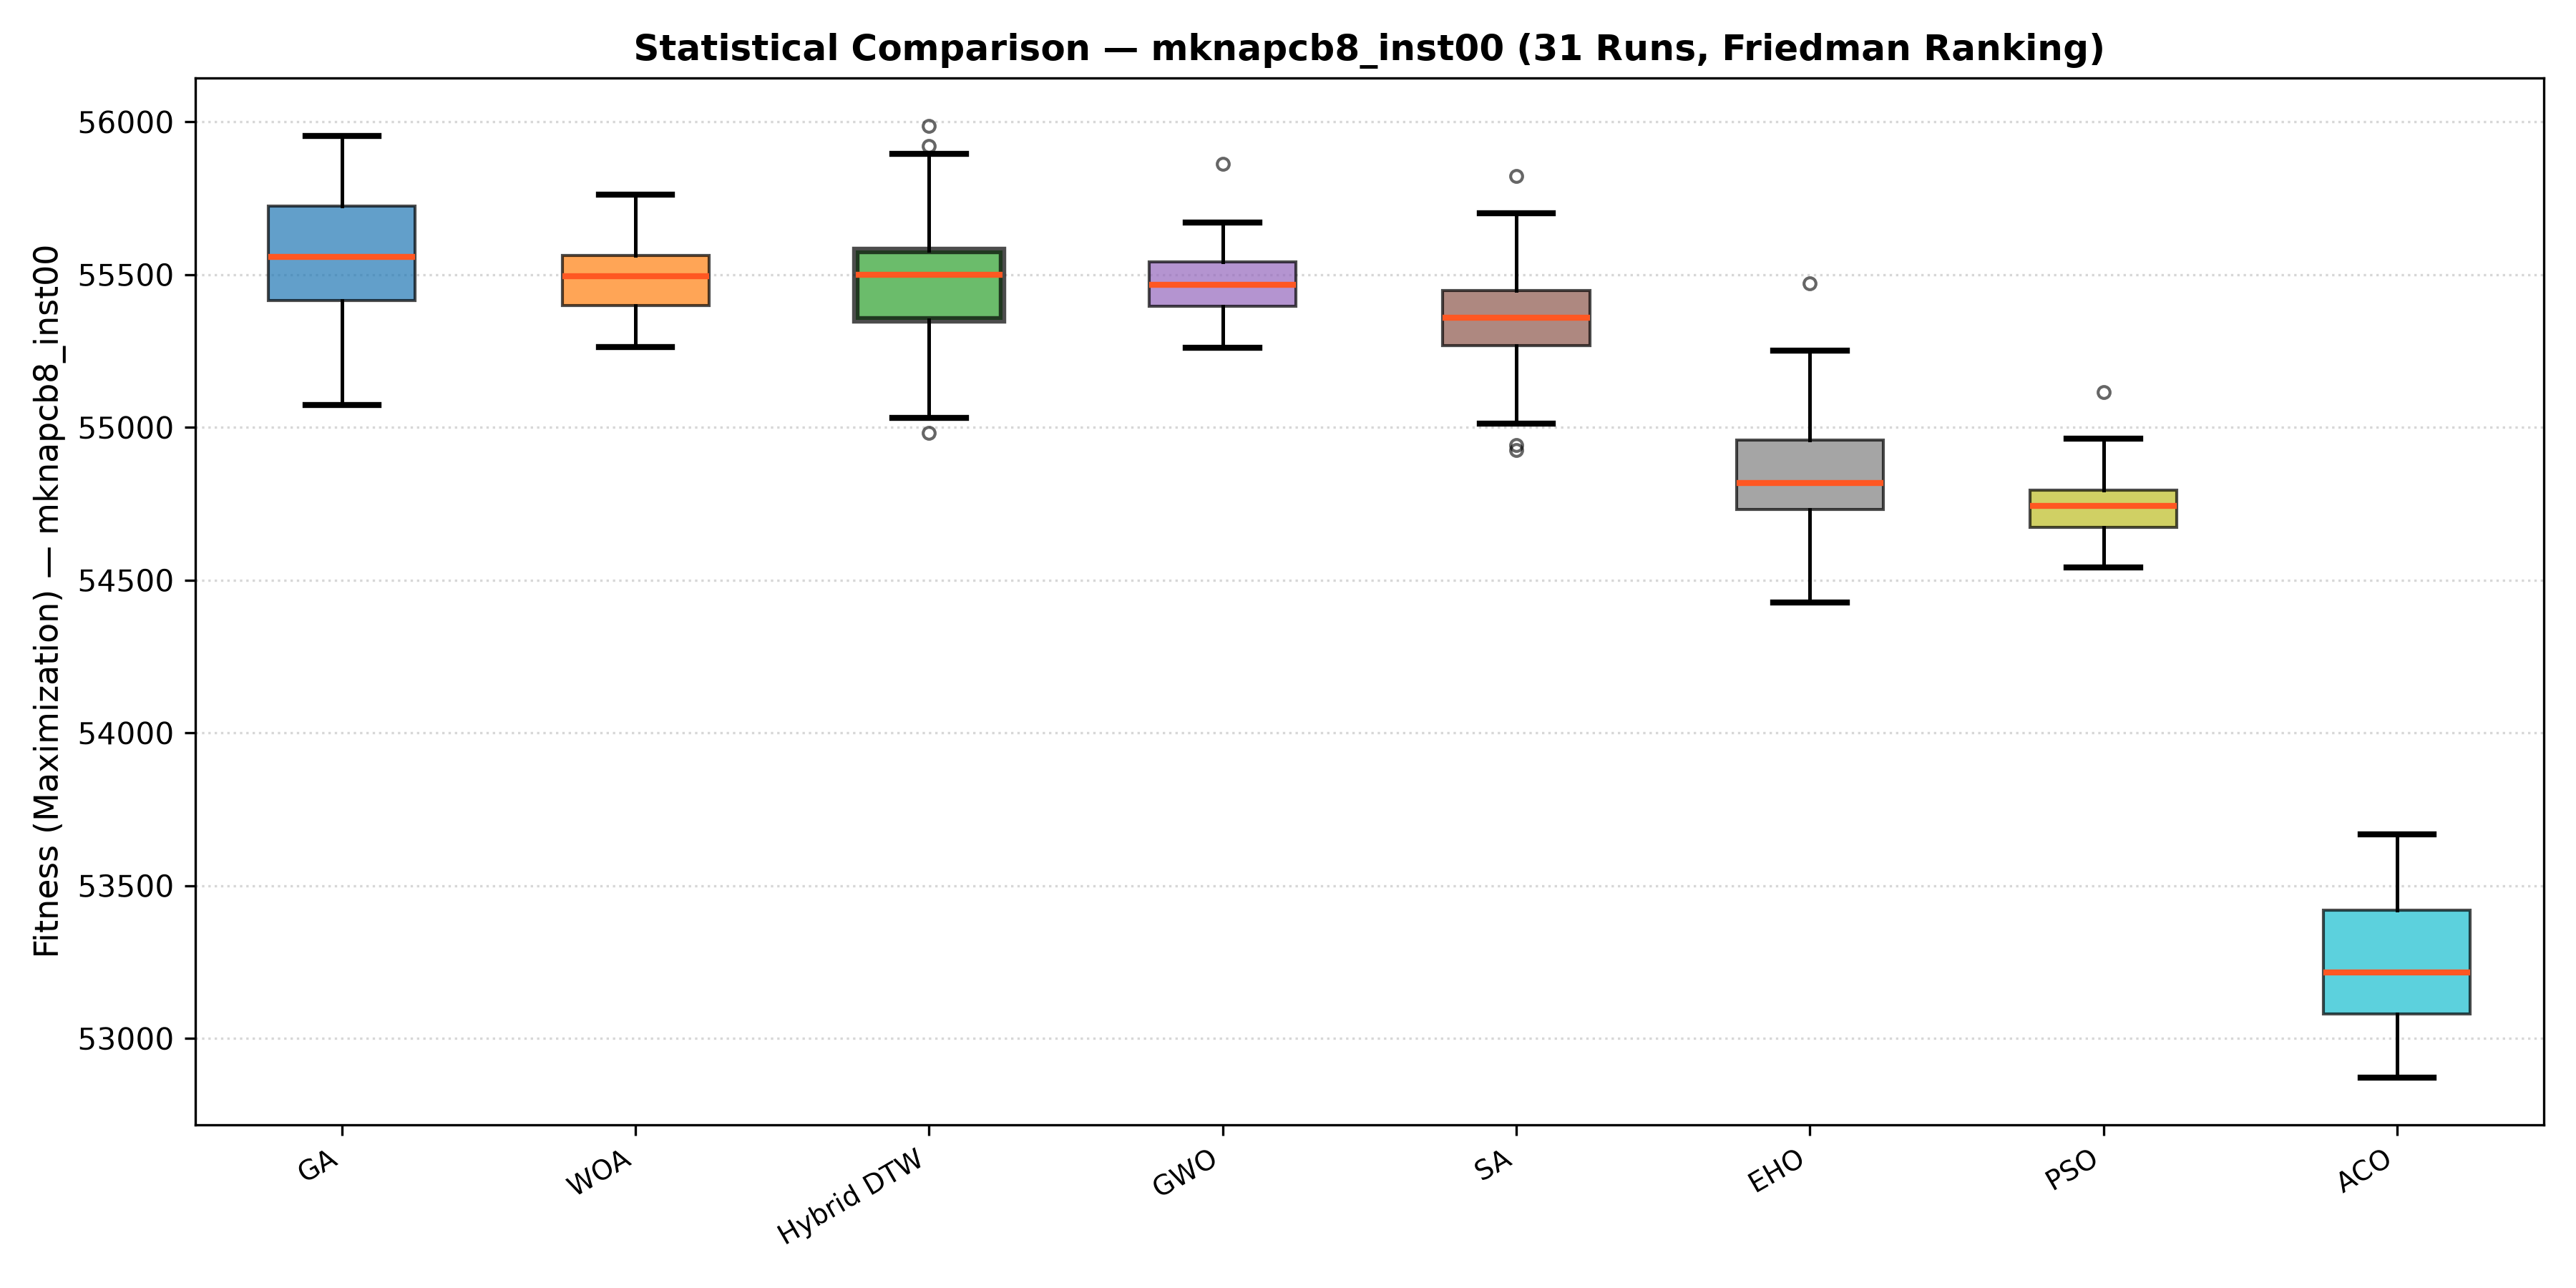
\includegraphics[width=0.32\textwidth]{imagenes_paper/mkp_dtw_3k_mknapcb8_comparativo_mh.png}}\hfill
\subfloat[Best-run convergence.]{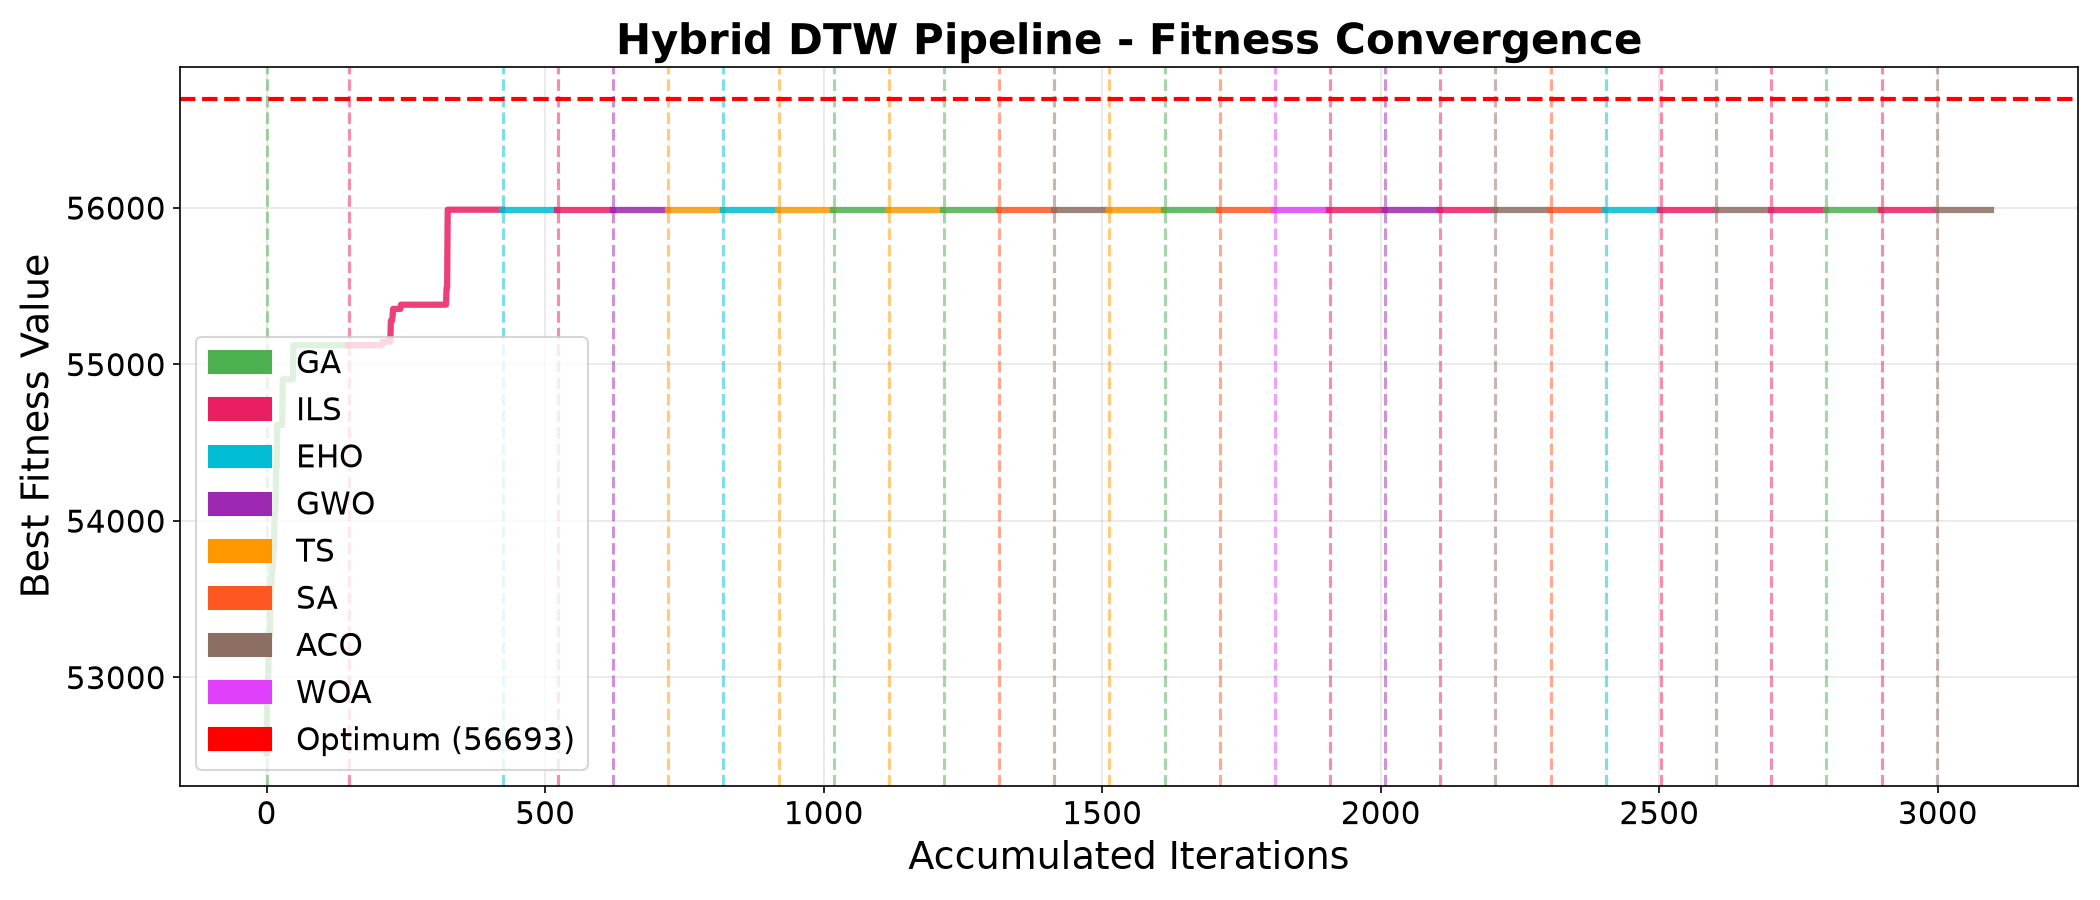
\includegraphics[width=0.32\textwidth]{imagenes_paper/mkp_dtw_3k_mknapcb8_convergencia.png}}\hfill
\subfloat[Elastic metric $\Delta=D_1-D_2$.]{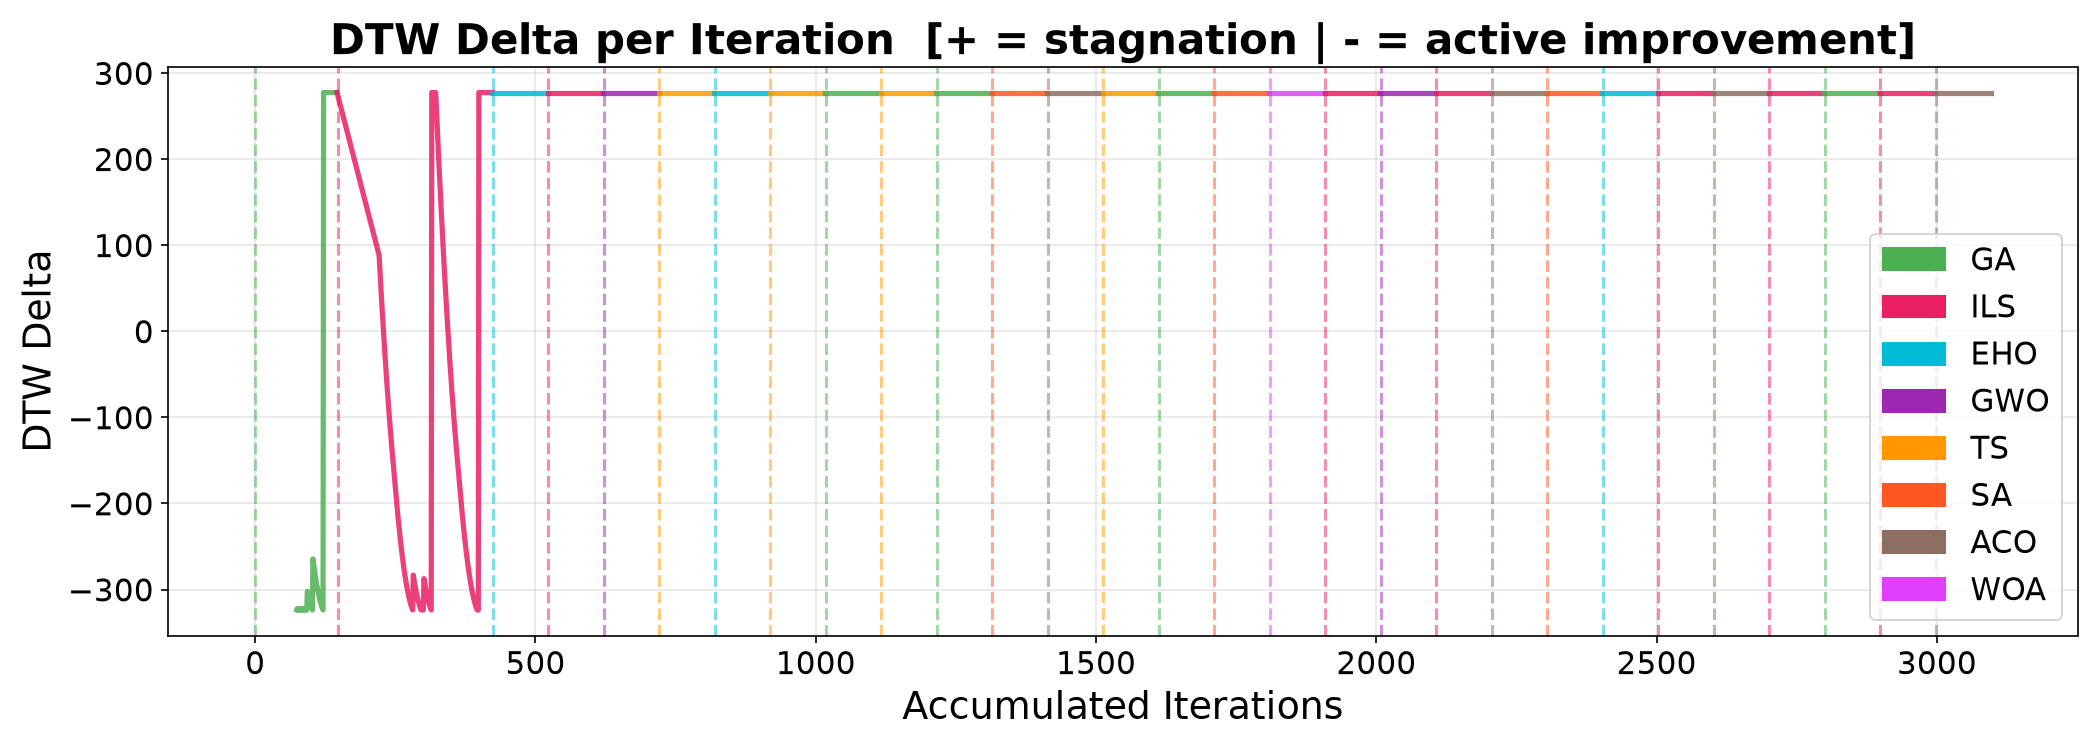
\includegraphics[width=0.32\textwidth]{imagenes_paper/mkp_dtw_3k_mknapcb8_delta.png}}
\caption{Diagnostic suite for instance \textbf{mknapcb8} ($n=250$, $m=30$) under the DTW framework with $T_{\max}=3{,}000$: (a)~final-fitness distribution over $N=31$ runs; (b)~convergence trajectory of the best run; (c)~elastic warping profile $\Delta$.}
\label{fig:mkp-best-cb8}
\end{figure}

% --- mknapcb9: DDTW, 3,000 iterations ---
\begin{figure}[htbp]
\centering
\subfloat[Metaheuristic comparison.]{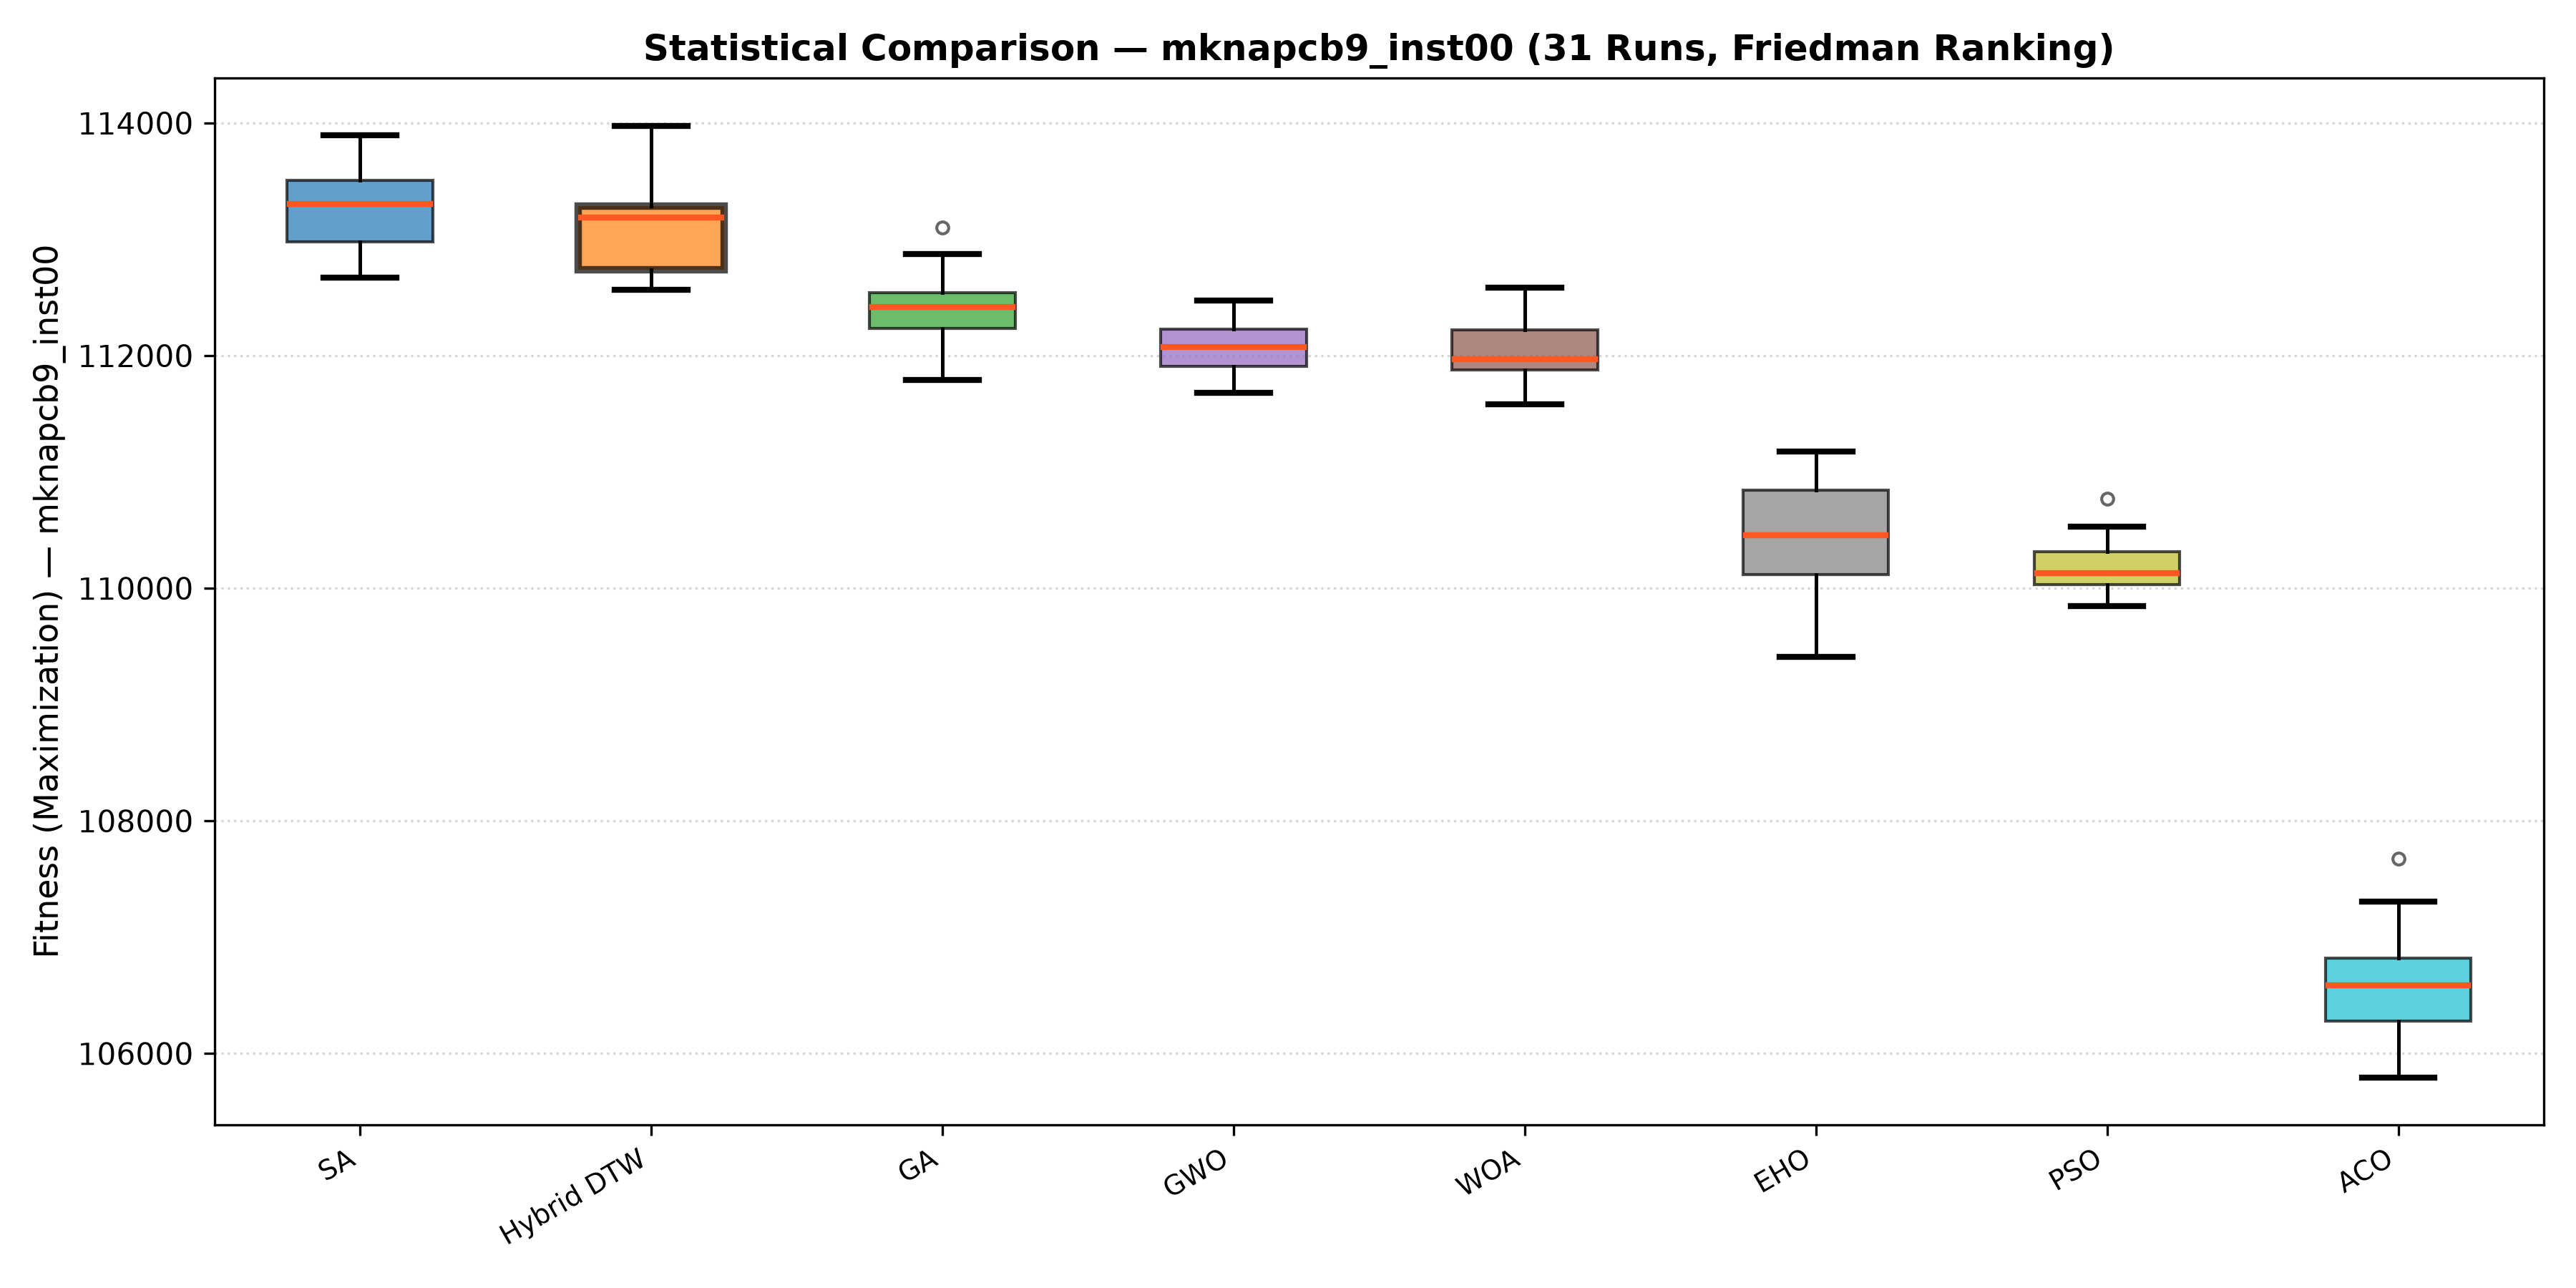
\includegraphics[width=0.32\textwidth]{imagenes_paper/mkp_ddtw_3k_mknapcb9_comparativo_mh.png}}\hfill
\subfloat[Best-run convergence.]{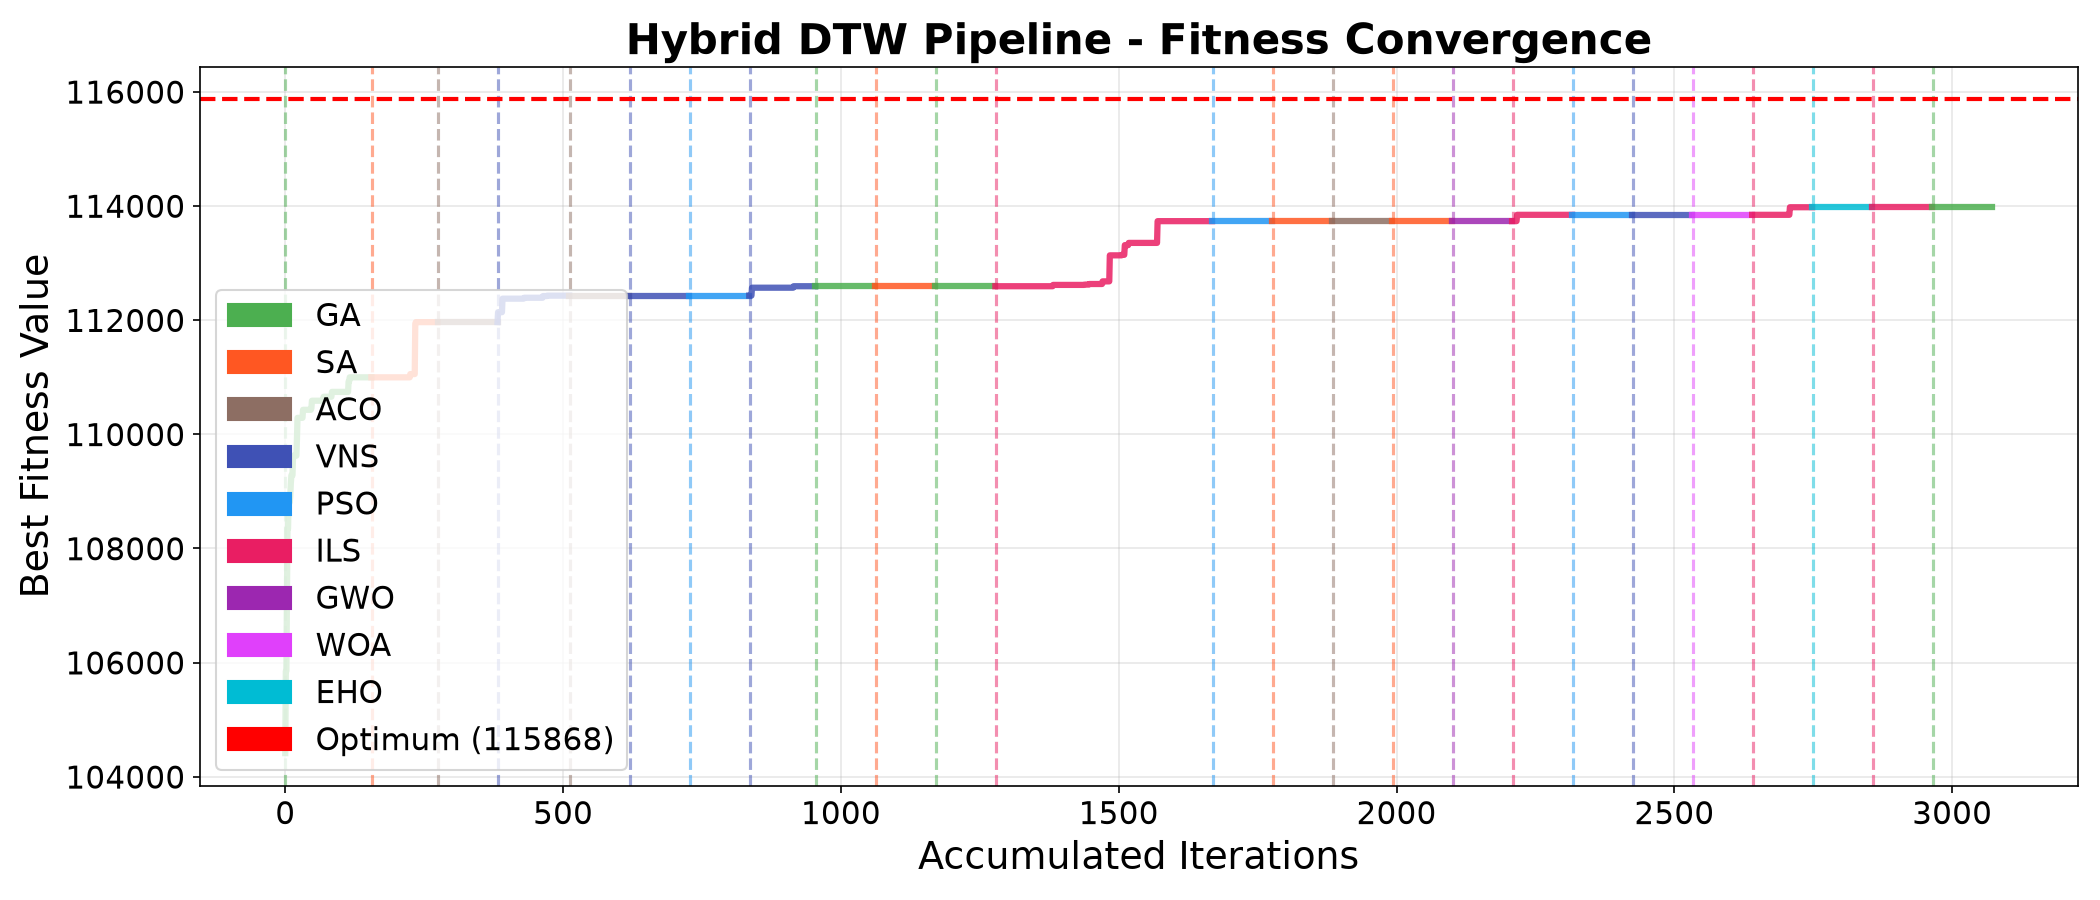
\includegraphics[width=0.32\textwidth]{imagenes_paper/mkp_ddtw_3k_mknapcb9_convergencia.png}}\hfill
\subfloat[Elastic metric $\Delta=D_1-D_2$.]{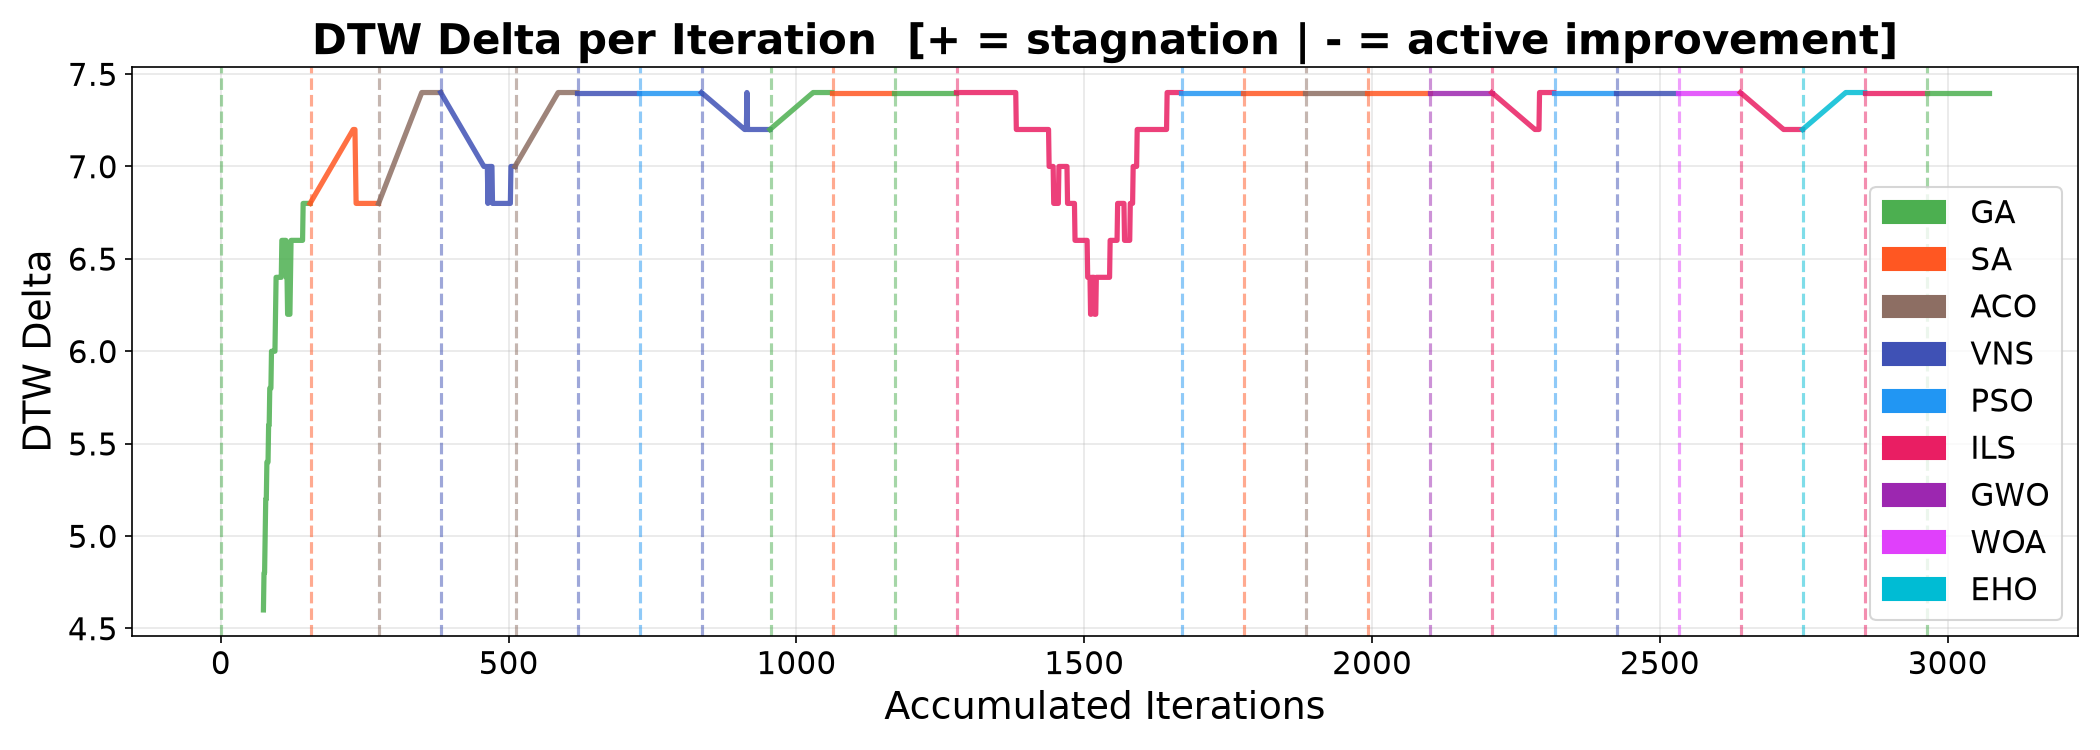
\includegraphics[width=0.32\textwidth]{imagenes_paper/mkp_ddtw_3k_mknapcb9_delta.png}}
\caption{Diagnostic suite for instance \textbf{mknapcb9} ($n=500$, $m=30$) under the DDTW framework with $T_{\max}=3{,}000$: (a)~final-fitness distribution over $N=31$ runs; (b)~convergence trajectory of the best run; (c)~elastic warping profile $\Delta$.}
\label{fig:mkp-best-cb9}
\end{figure}

% Required packages: graphicx, subfig (or subcaption with \subfloat redefined).

% Each figure shows the best-performing framework configuration for the
% corresponding instance, selected by highest mean fitness over 31 runs.
% DTW--3K is best for mknapcb1 and mknapcb3--mknapcb8;
% DDTW--3K is best for mknapcb2 and mknapcb9.

Figures~\ref{fig:mkp-best-cb1}--\ref{fig:mkp-best-cb9} present the
diagnostic suite for each of the nine Chu--Beasley MKP instances under its
best-performing framework configuration, selected by highest mean fitness
over the 31 runs, with corresponding executions treated as paired. DTW with $T_{\max}=3{,}000$ achieved the
highest mean in seven instances (mknapcb1 and mknapcb3--mknapcb8), while
DDTW with $T_{\max}=3{,}000$ was superior for mknapcb2 and mknapcb9.
Each figure comprises three panels: (a)~a box-plot comparing the
final-fitness distributions of the hybrid framework against the standalone
metaheuristics over the 31 runs, allowing visual assessment of both central
tendency and dispersion; (b)~the convergence trajectory of the best run,
showing the evolution of the incumbent fitness along with the solver
transitions triggered by the stagnation monitor; and (c)~the elastic
warping profile $\Delta = D_1 - D_2$, where positive values indicate
detected stagnation phases and negative values correspond to periods of
active improvement.

% --- mknapcb1: DTW, 3,000 iterations ---
\begin{figure}[htbp]
\centering
\subfloat[Metaheuristic comparison.]{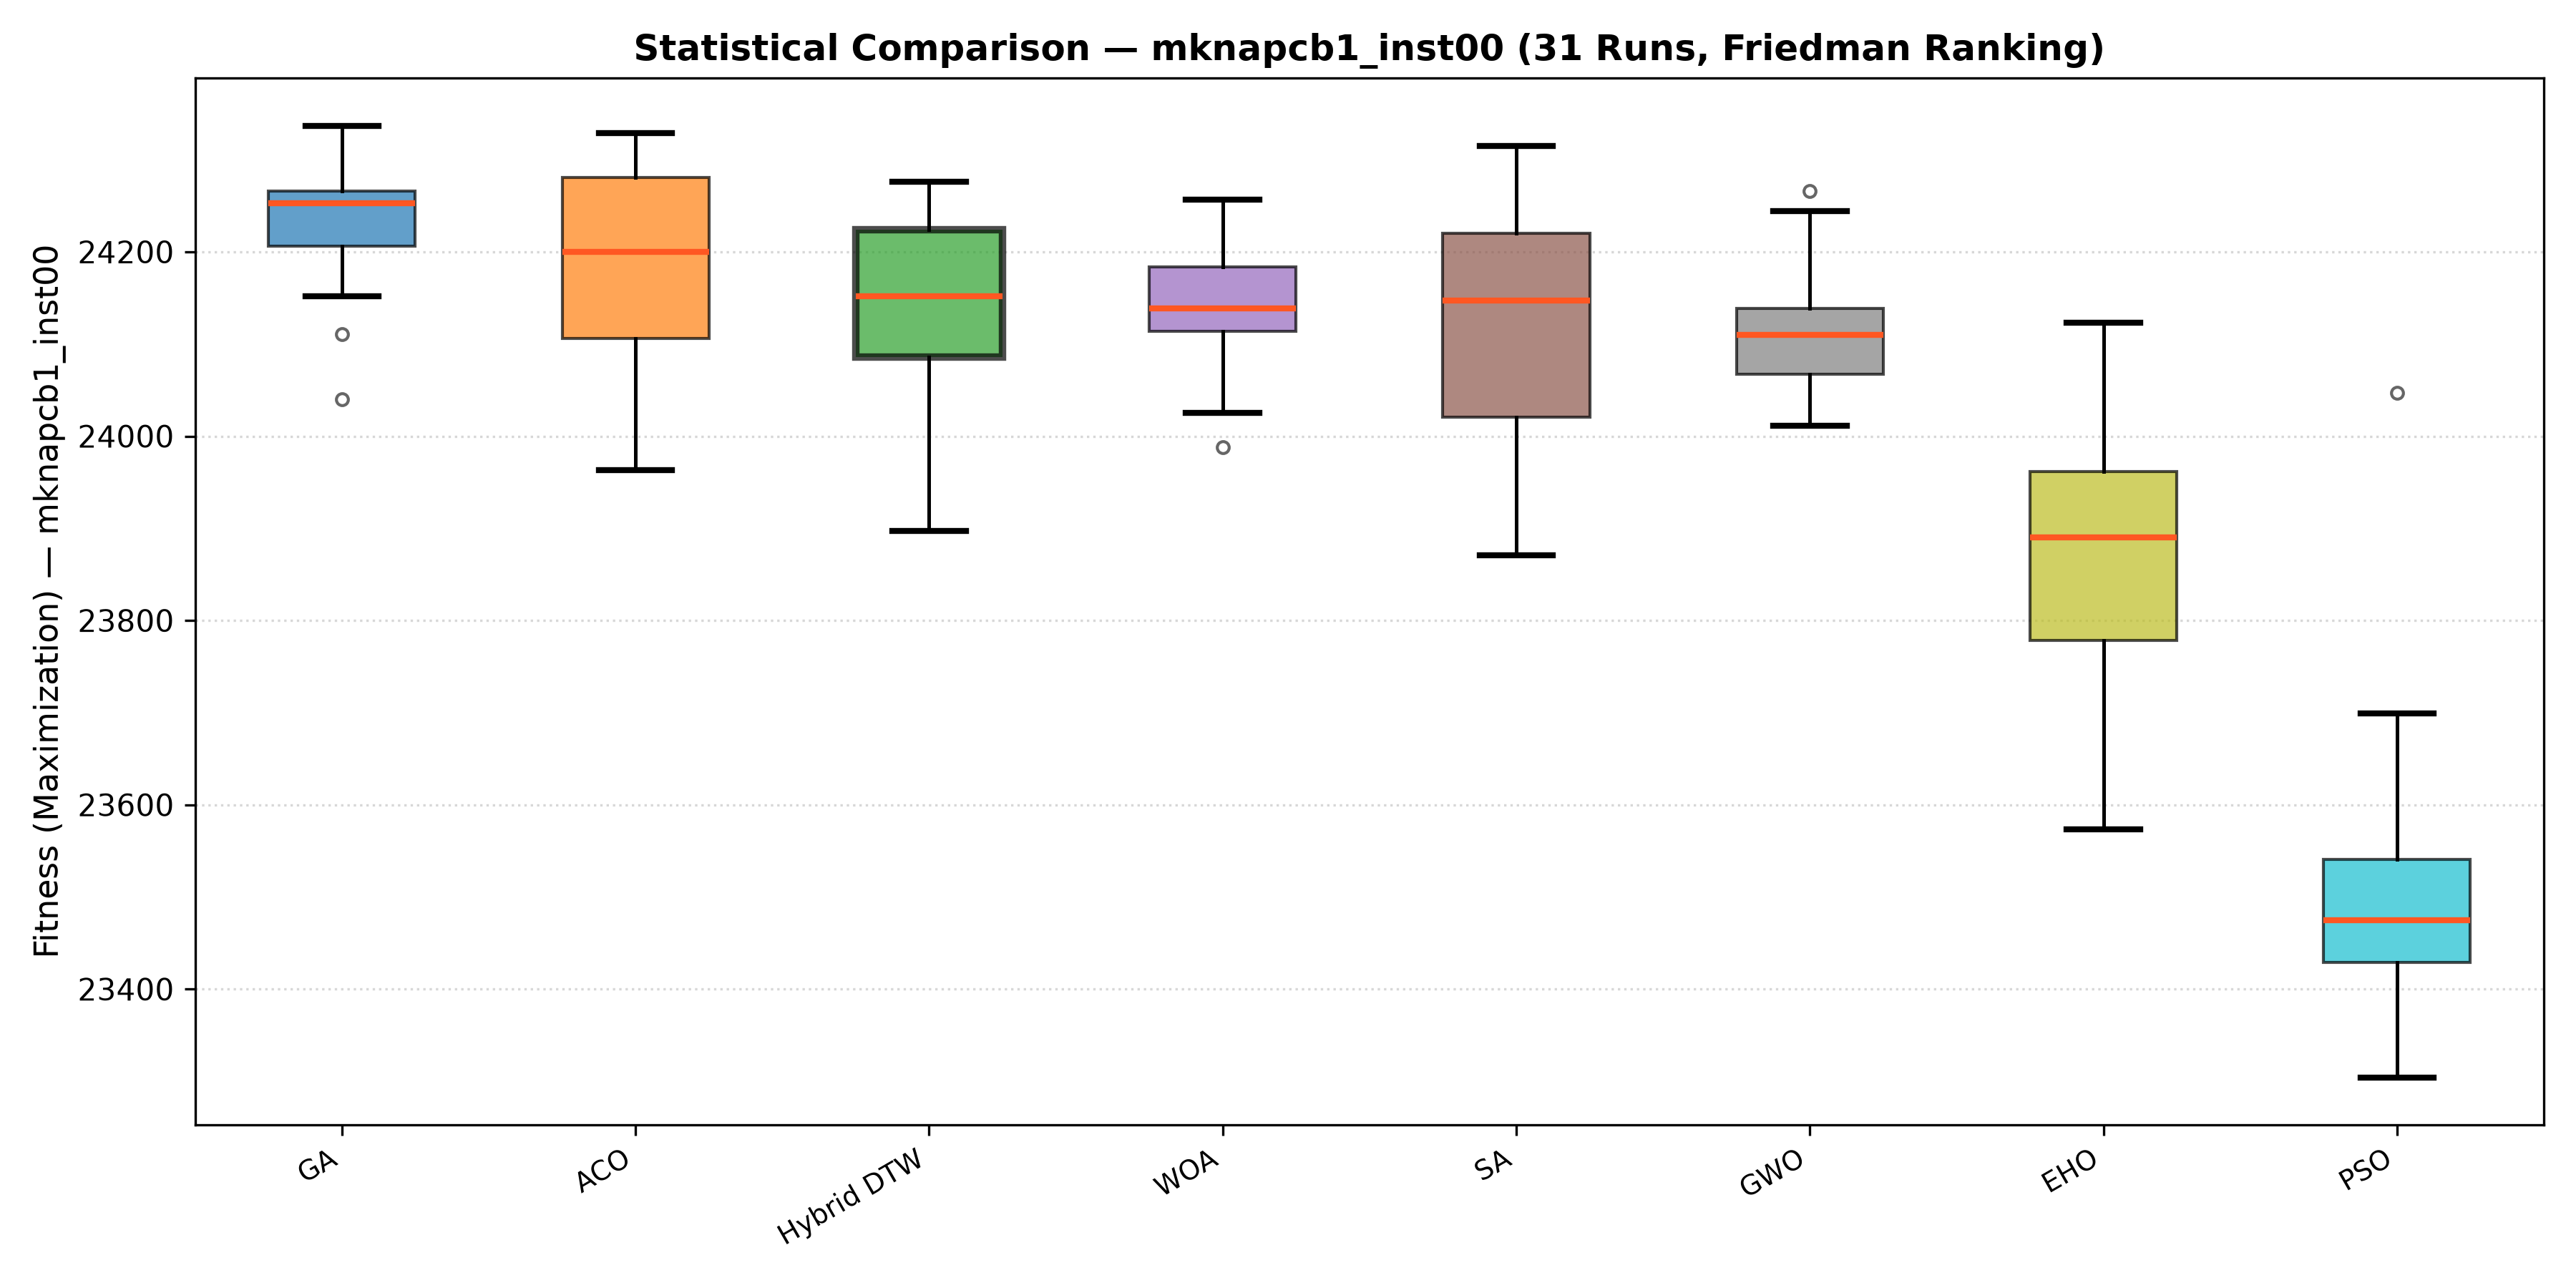
\includegraphics[width=0.32\textwidth]{imagenes_paper/mkp_dtw_3k_mknapcb1_comparativo_mh.png}}\hfill
\subfloat[Best-run convergence.]{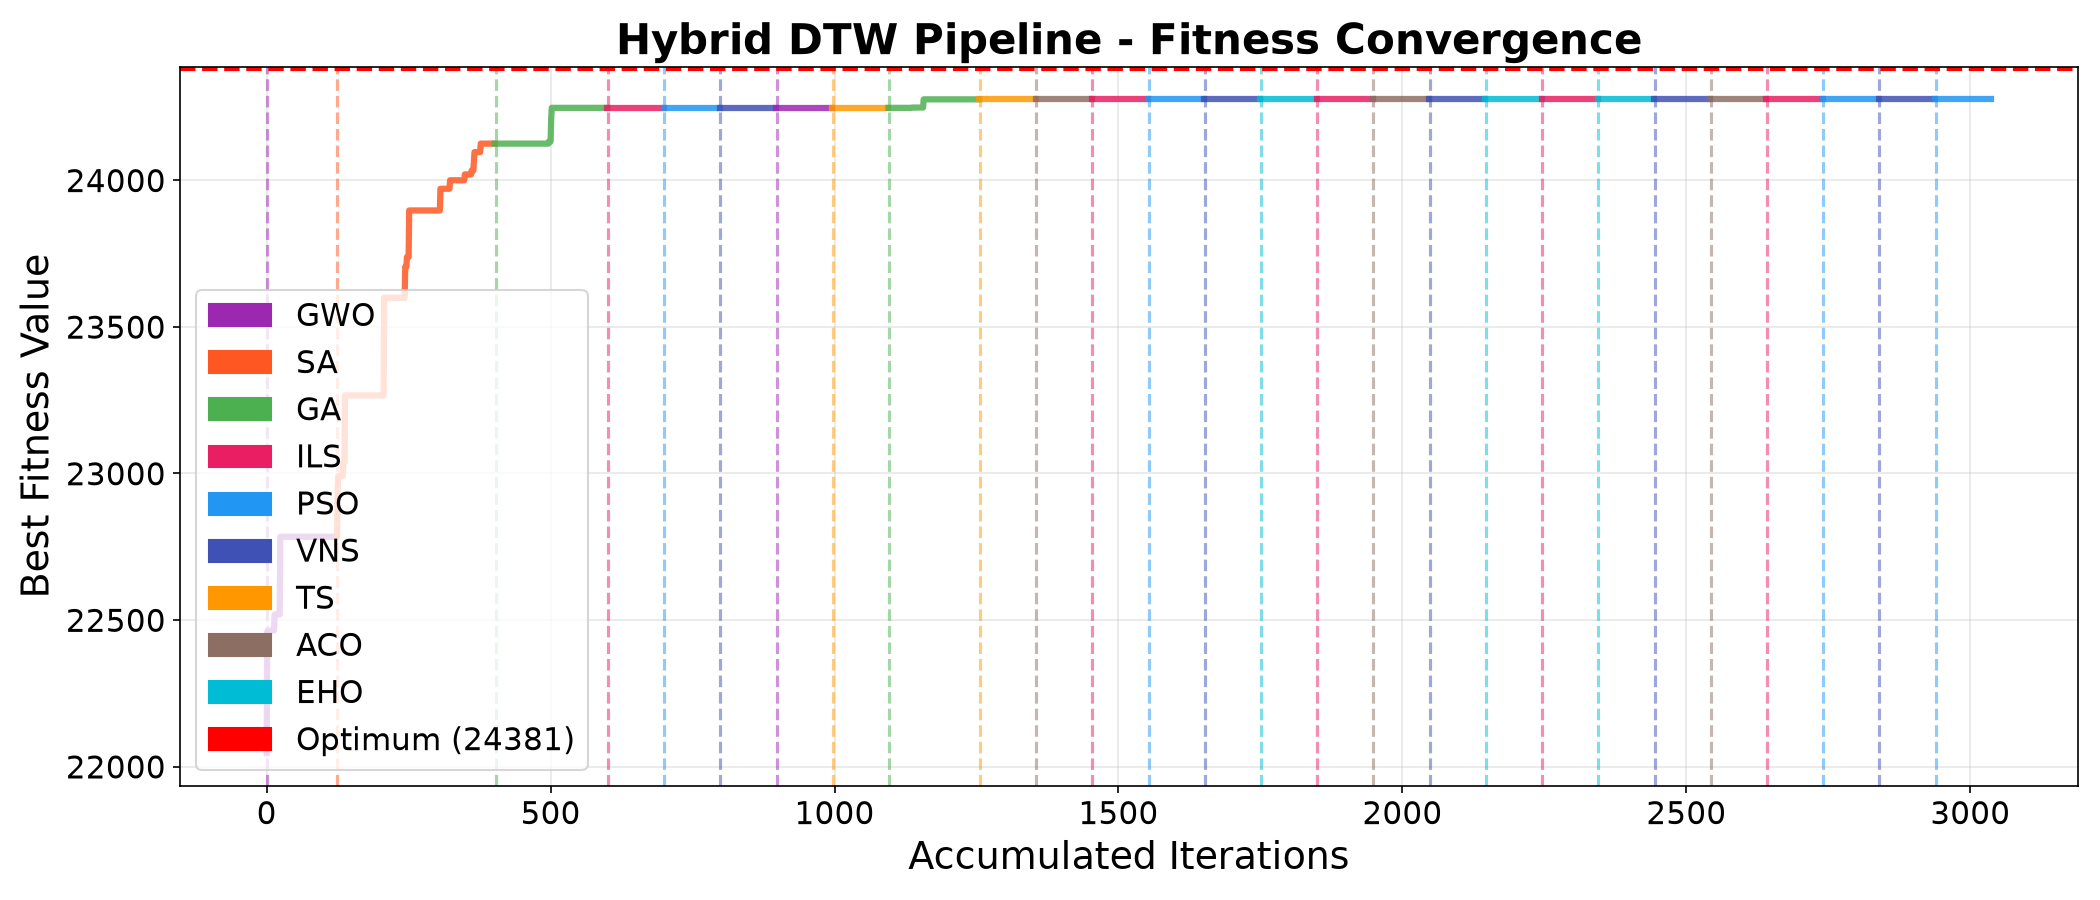
\includegraphics[width=0.32\textwidth]{imagenes_paper/mkp_dtw_3k_mknapcb1_convergencia.png}}\hfill
\subfloat[Elastic metric $\Delta=D_1-D_2$.]{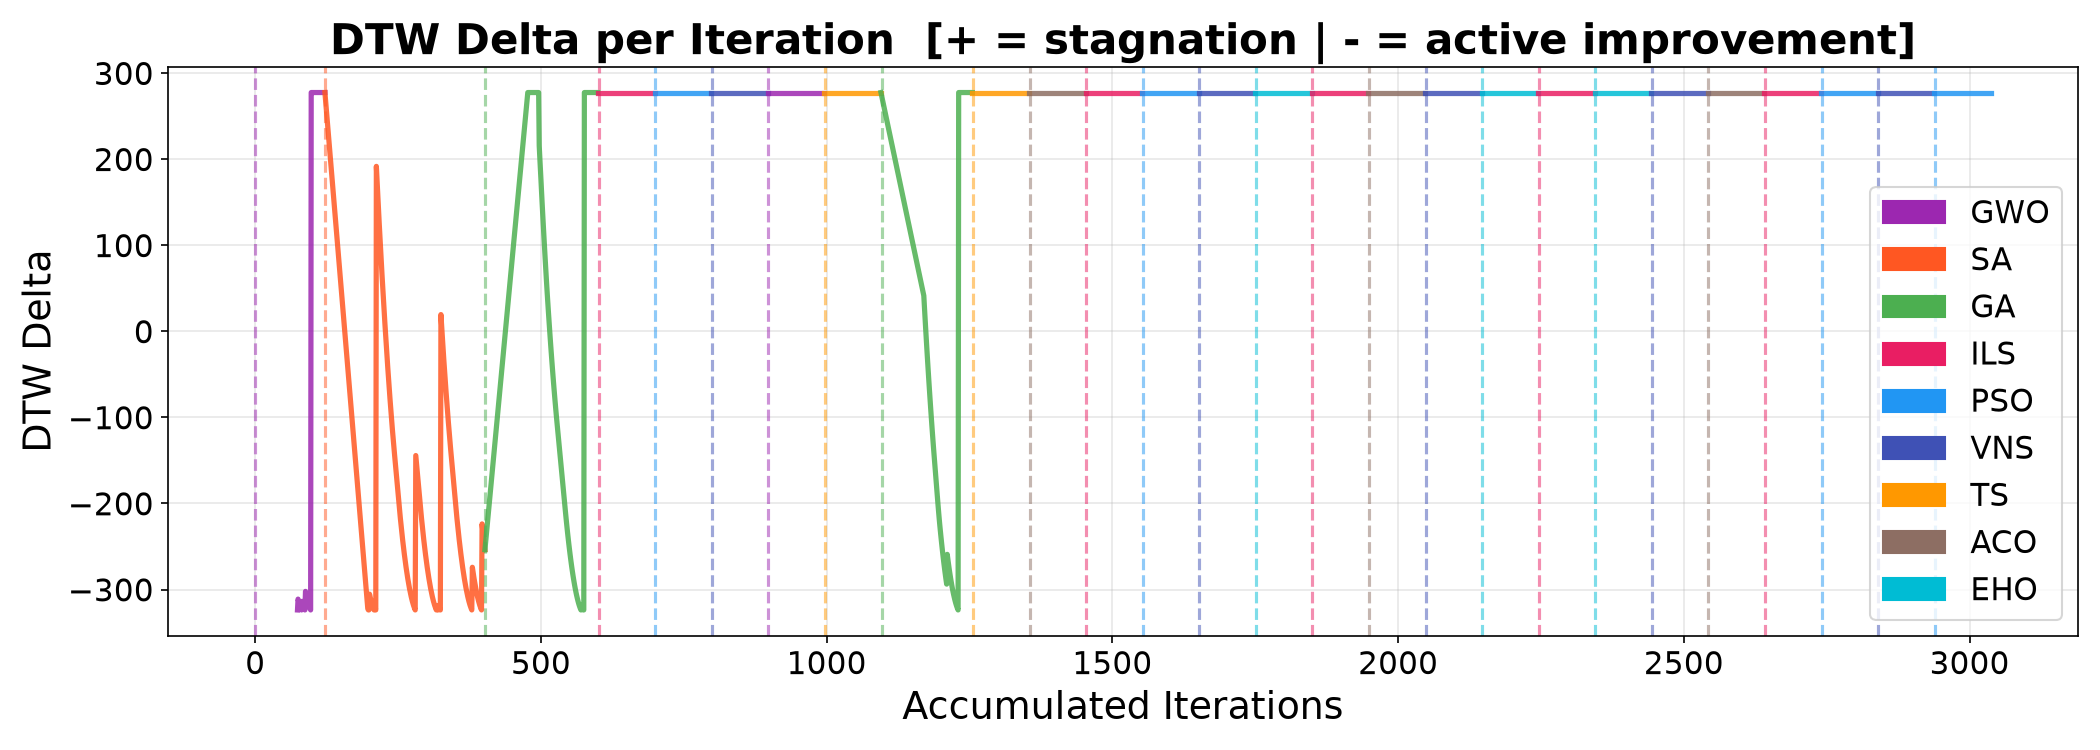
\includegraphics[width=0.32\textwidth]{imagenes_paper/mkp_dtw_3k_mknapcb1_delta.png}}
\caption{Diagnostic suite for instance \textbf{mknapcb1} ($n=100$, $m=5$) under the DTW framework with $T_{\max}=3{,}000$: (a)~final-fitness distribution over $N=31$ runs; (b)~convergence trajectory of the best run; (c)~elastic warping profile $\Delta$.}
\label{fig:mkp-best-cb1}
\end{figure}

% --- mknapcb2: DDTW, 3,000 iterations ---
\begin{figure}[htbp]
\centering
\subfloat[Metaheuristic comparison.]{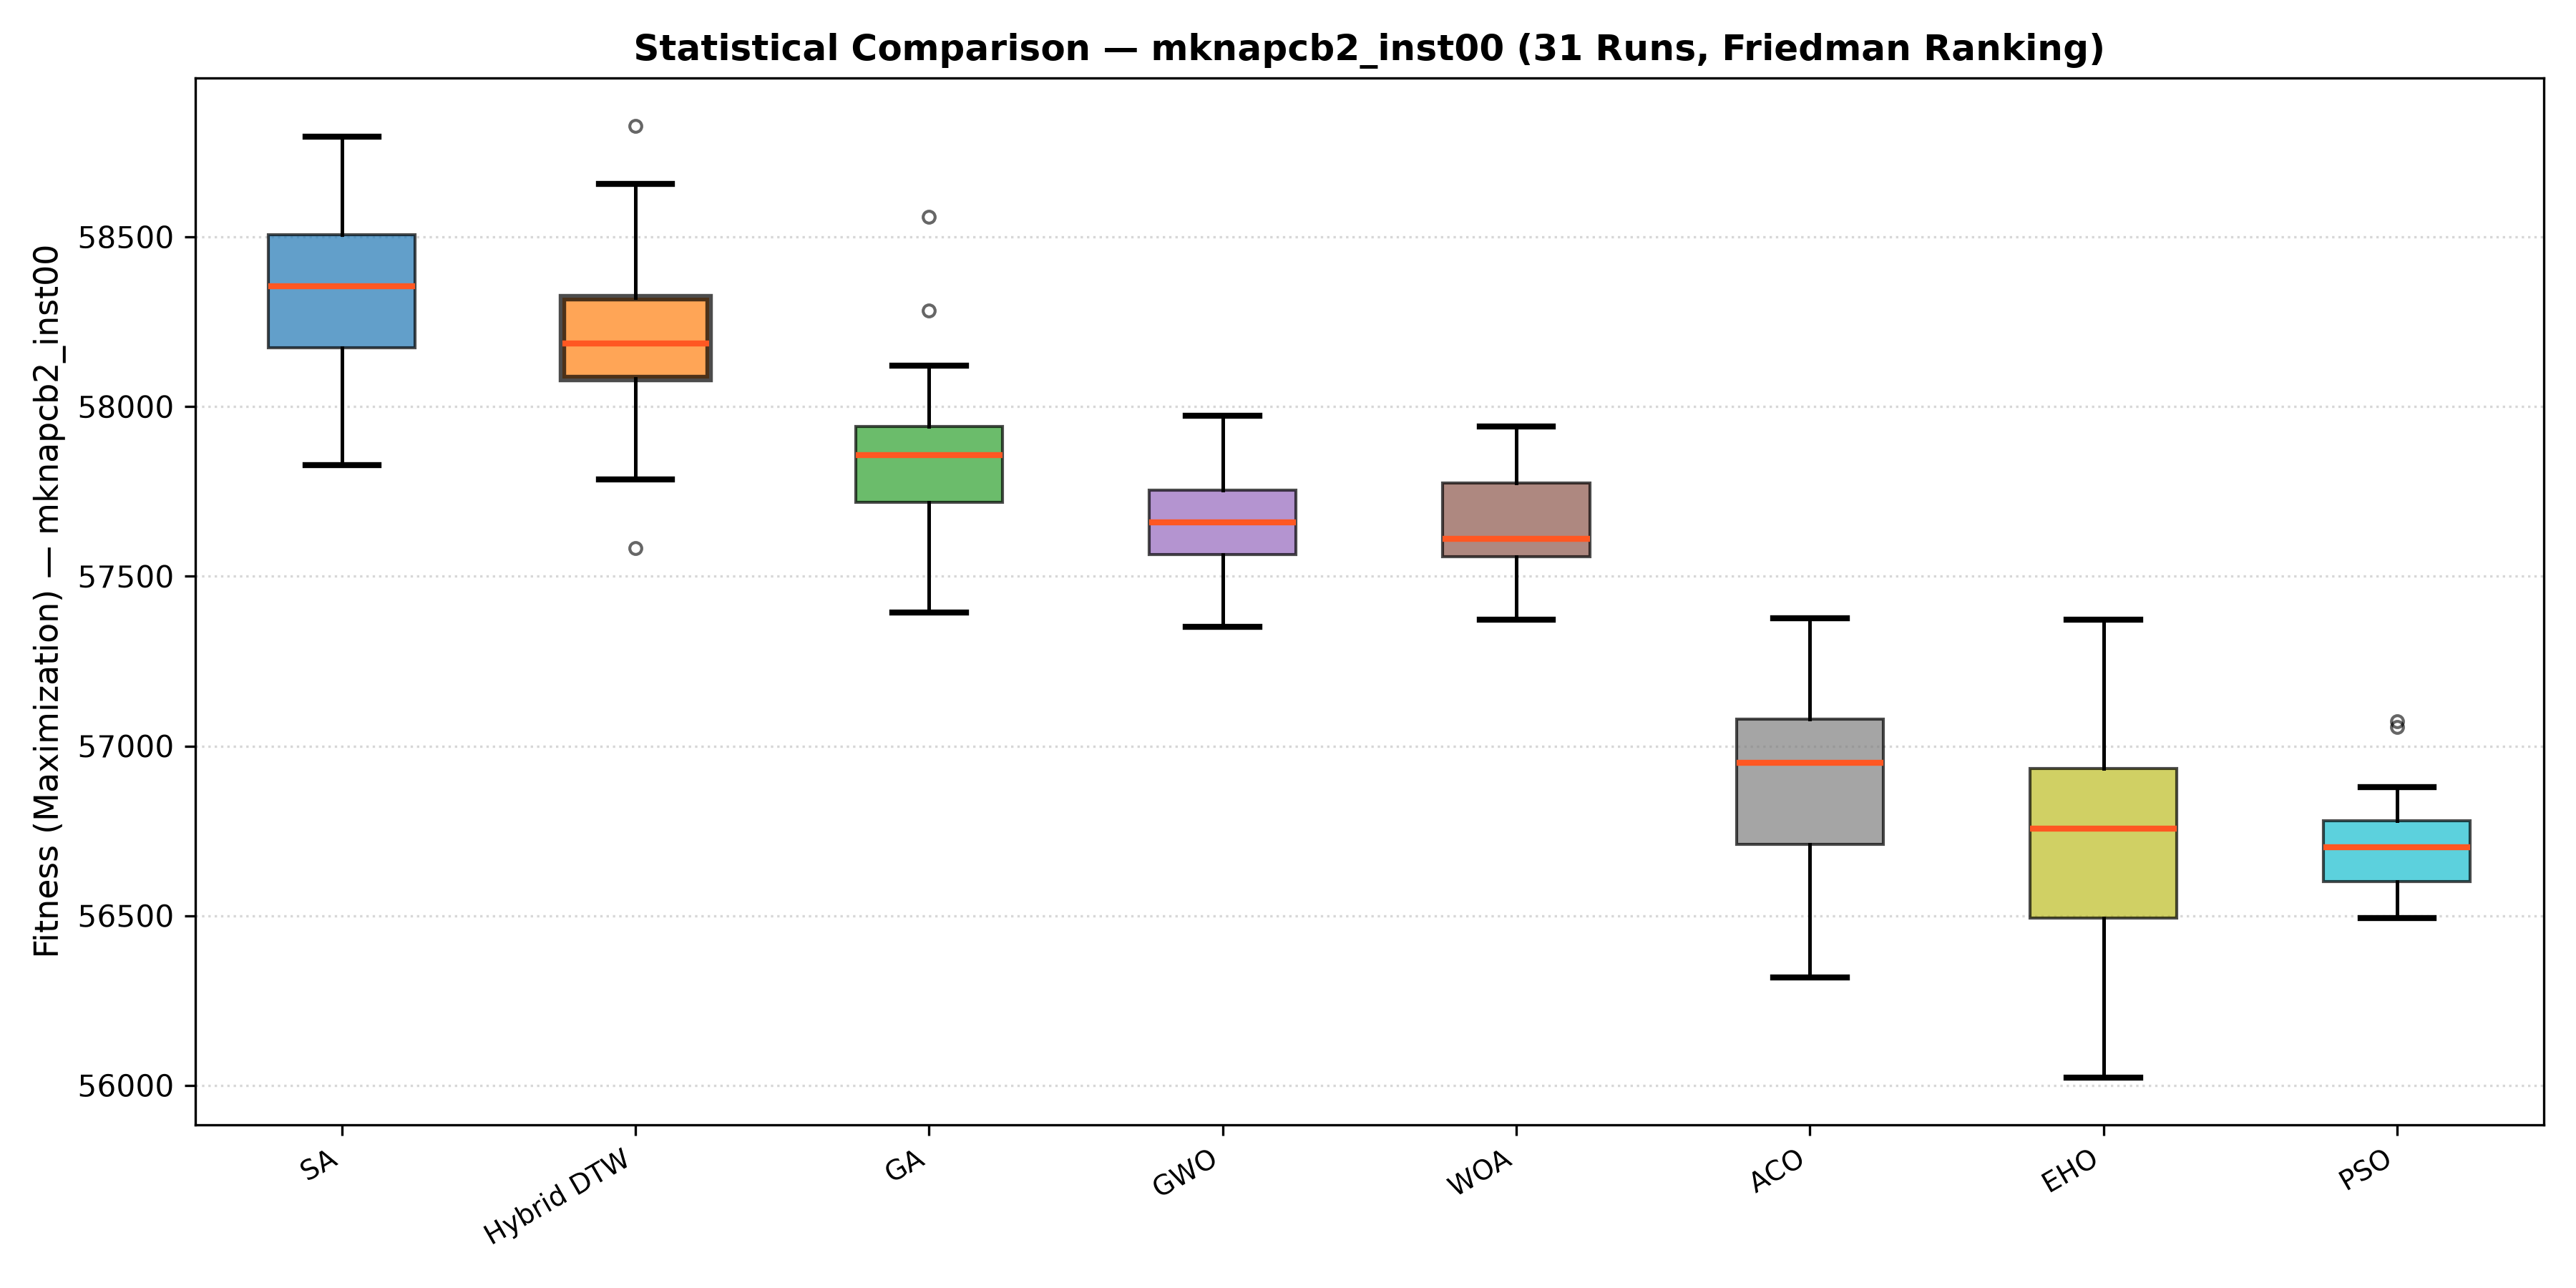
\includegraphics[width=0.32\textwidth]{imagenes_paper/mkp_ddtw_3k_mknapcb2_comparativo_mh.png}}\hfill
\subfloat[Best-run convergence.]{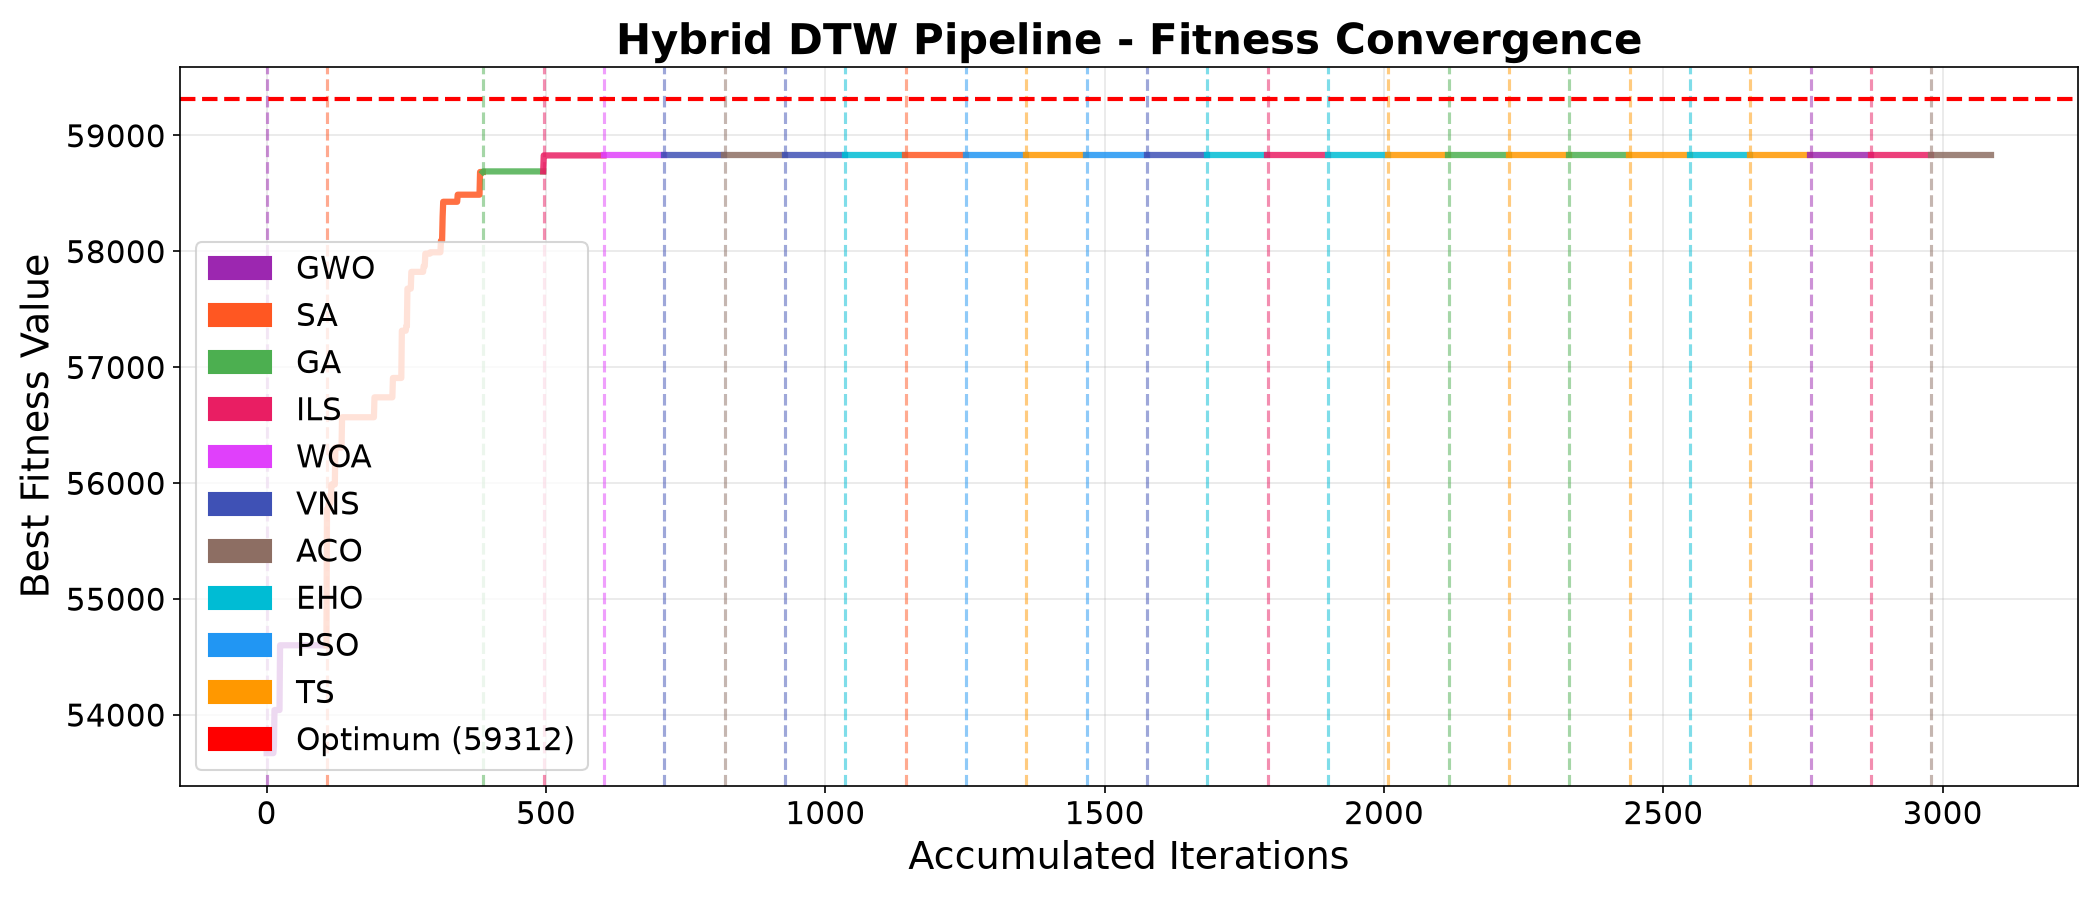
\includegraphics[width=0.32\textwidth]{imagenes_paper/mkp_ddtw_3k_mknapcb2_convergencia.png}}\hfill
\subfloat[Elastic metric $\Delta=D_1-D_2$.]{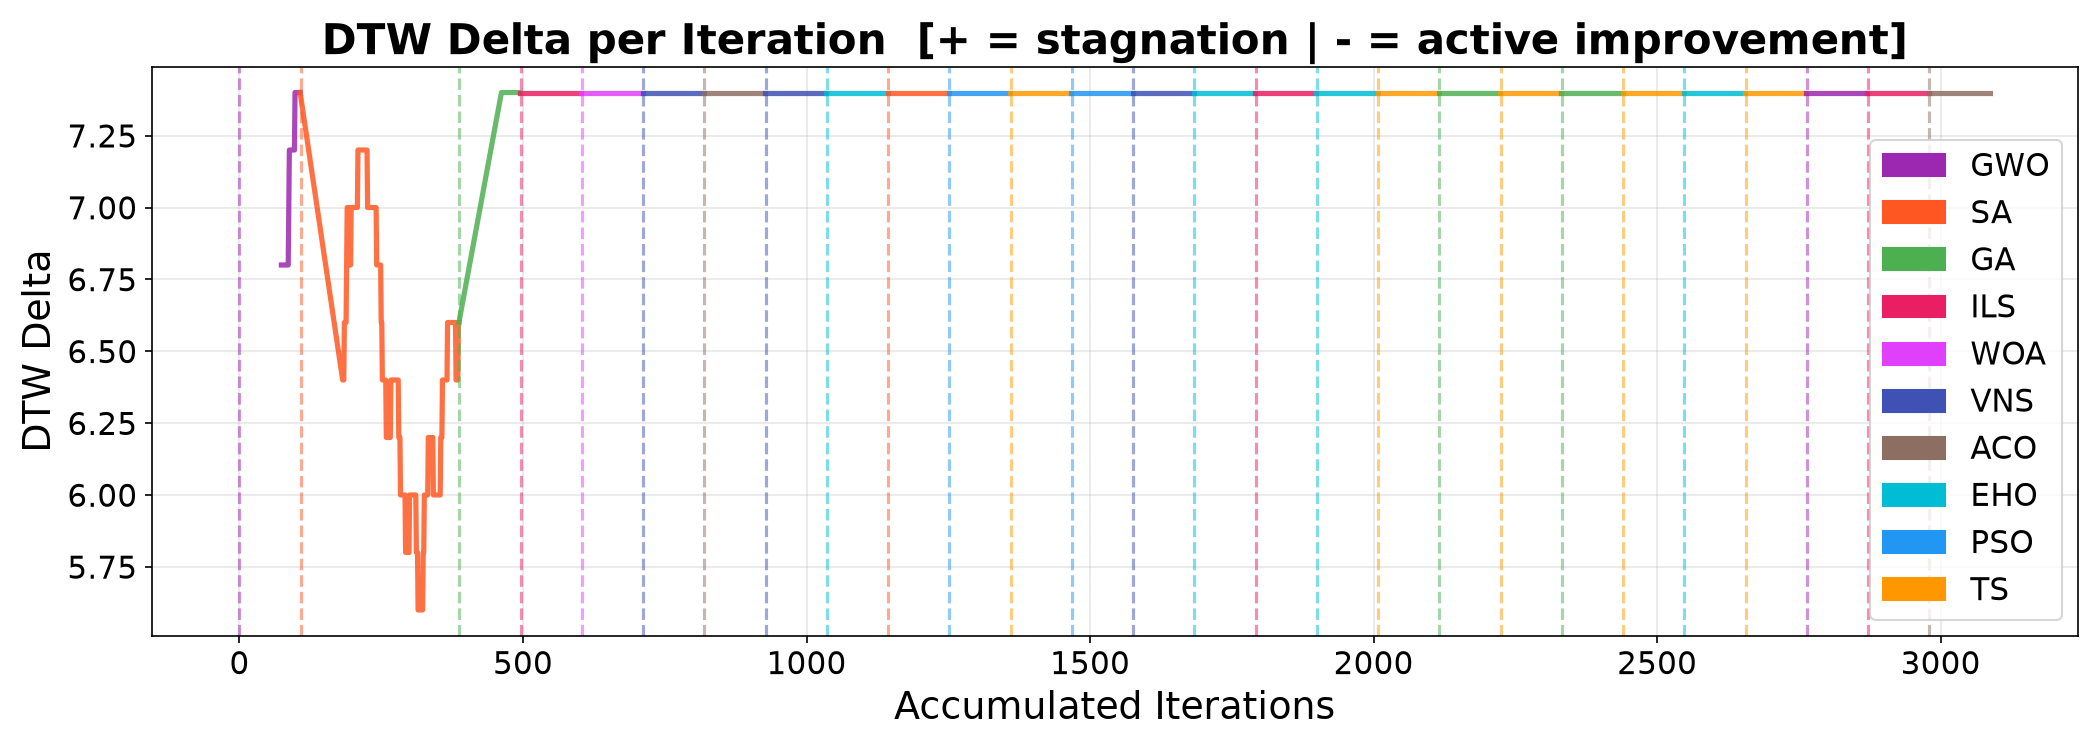
\includegraphics[width=0.32\textwidth]{imagenes_paper/mkp_ddtw_3k_mknapcb2_delta.png}}
\caption{Diagnostic suite for instance \textbf{mknapcb2} ($n=250$, $m=5$) under the DDTW framework with $T_{\max}=3{,}000$: (a)~final-fitness distribution over $N=31$ runs; (b)~convergence trajectory of the best run; (c)~elastic warping profile $\Delta$.}
\label{fig:mkp-best-cb2}
\end{figure}

% --- mknapcb3: DTW, 3,000 iterations ---
\begin{figure}[htbp]
\centering
\subfloat[Metaheuristic comparison.]{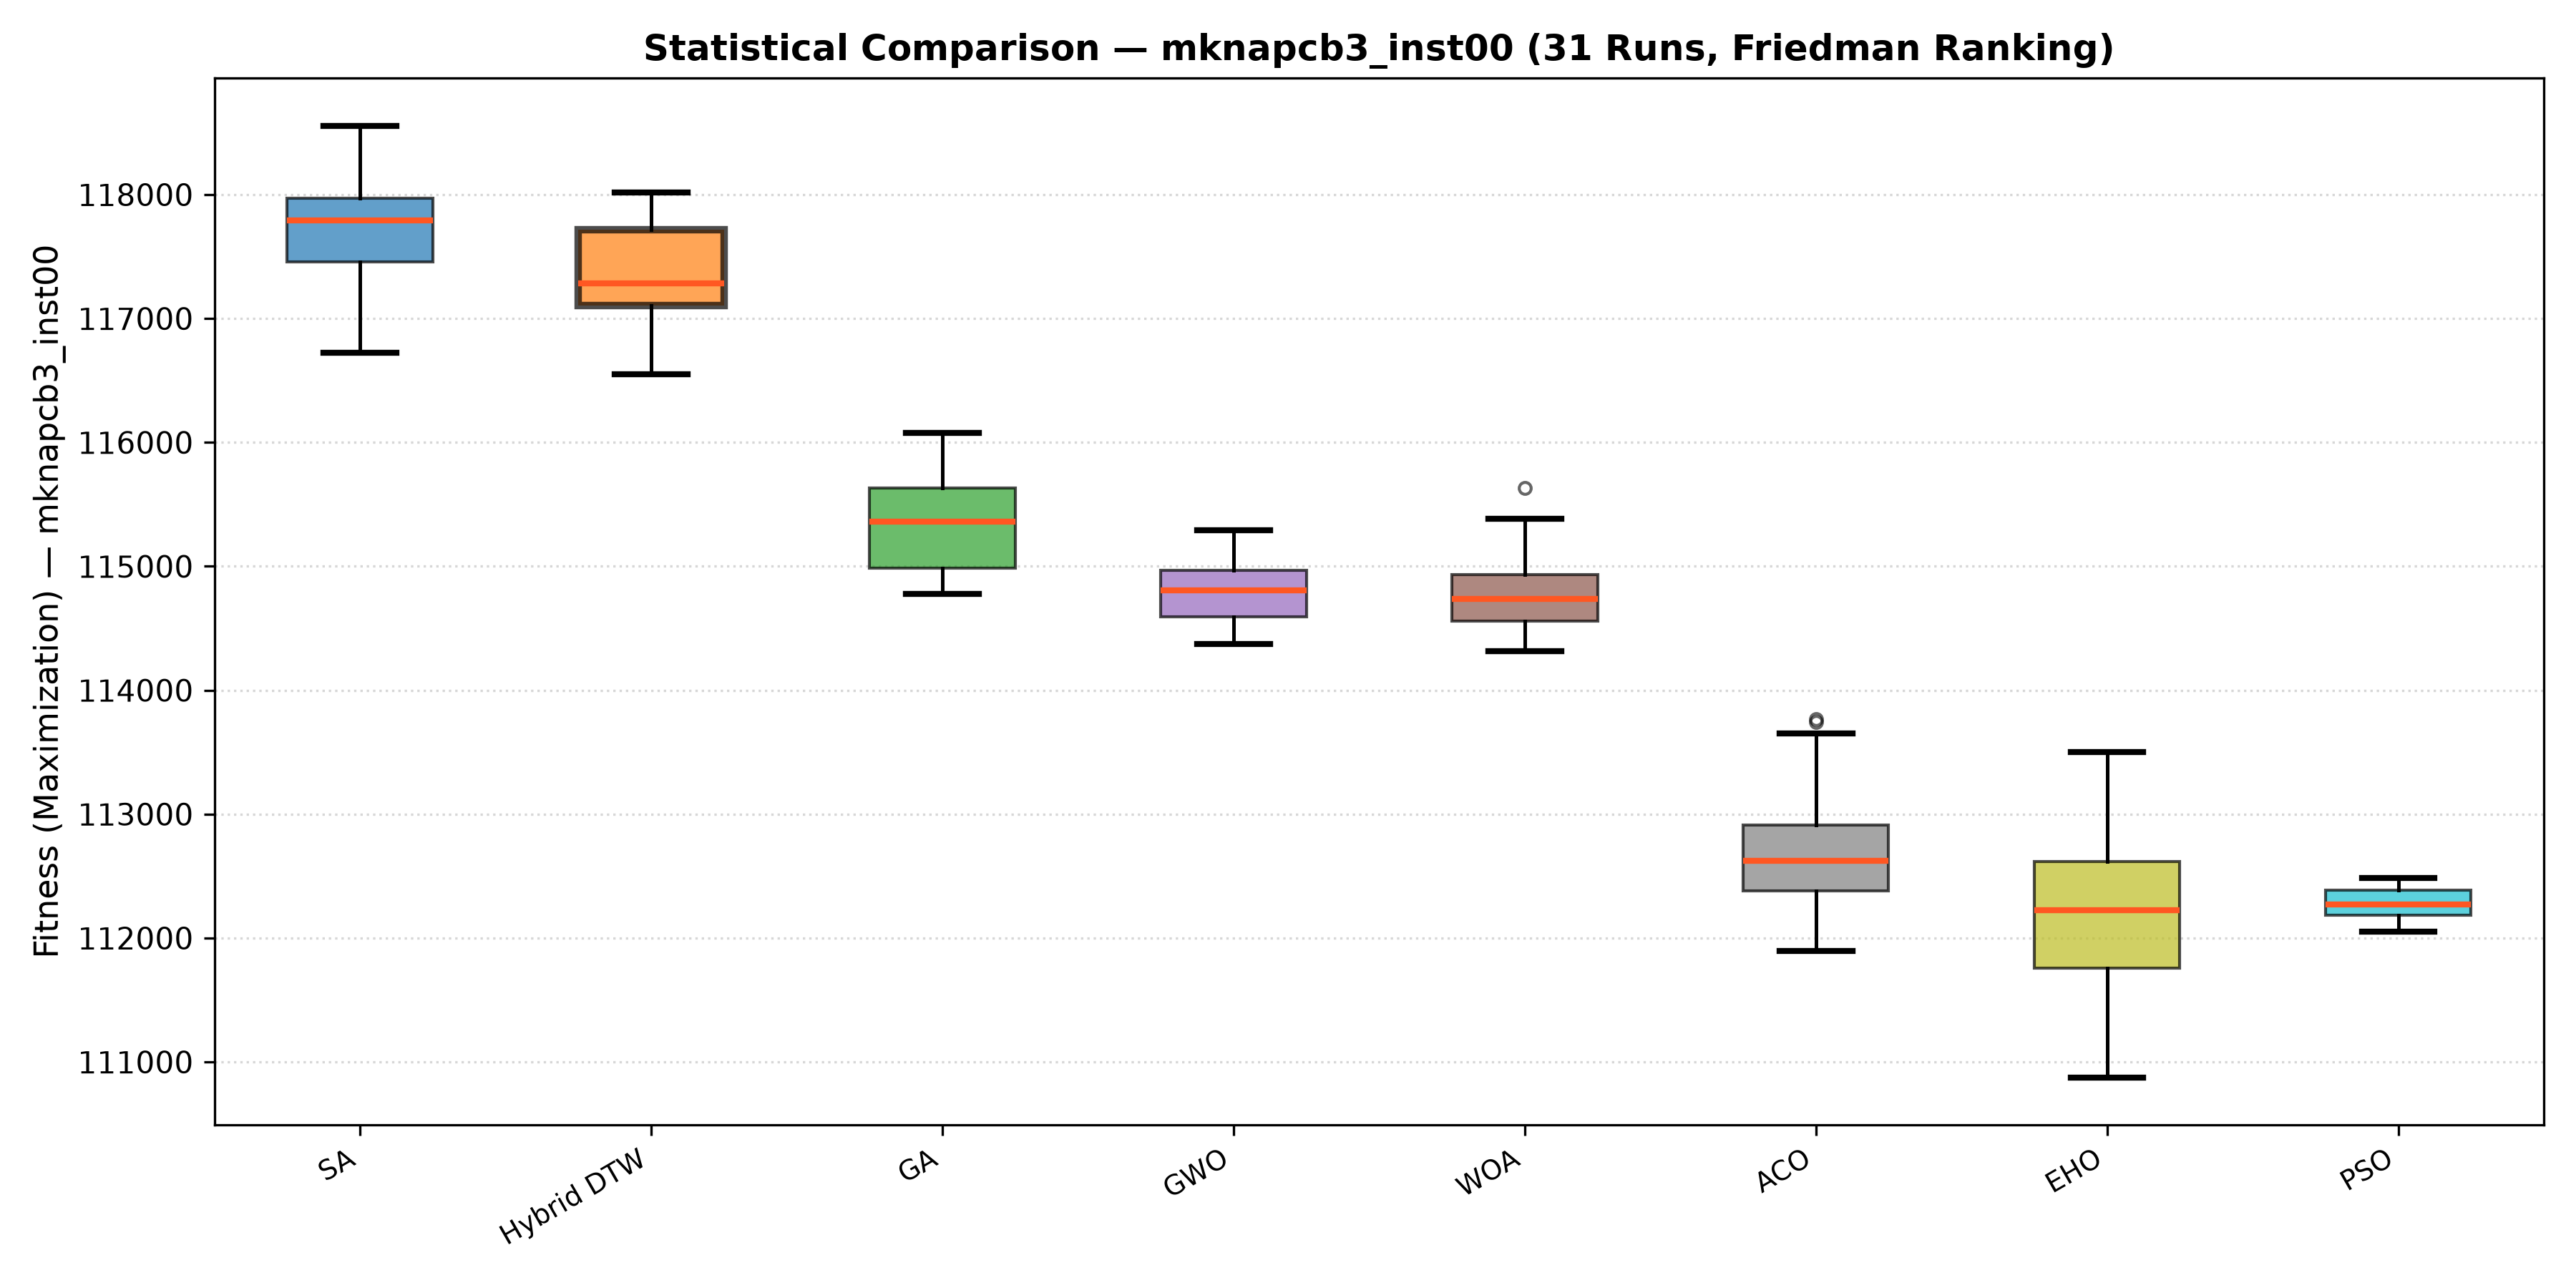
\includegraphics[width=0.32\textwidth]{imagenes_paper/mkp_dtw_3k_mknapcb3_comparativo_mh.png}}\hfill
\subfloat[Best-run convergence.]{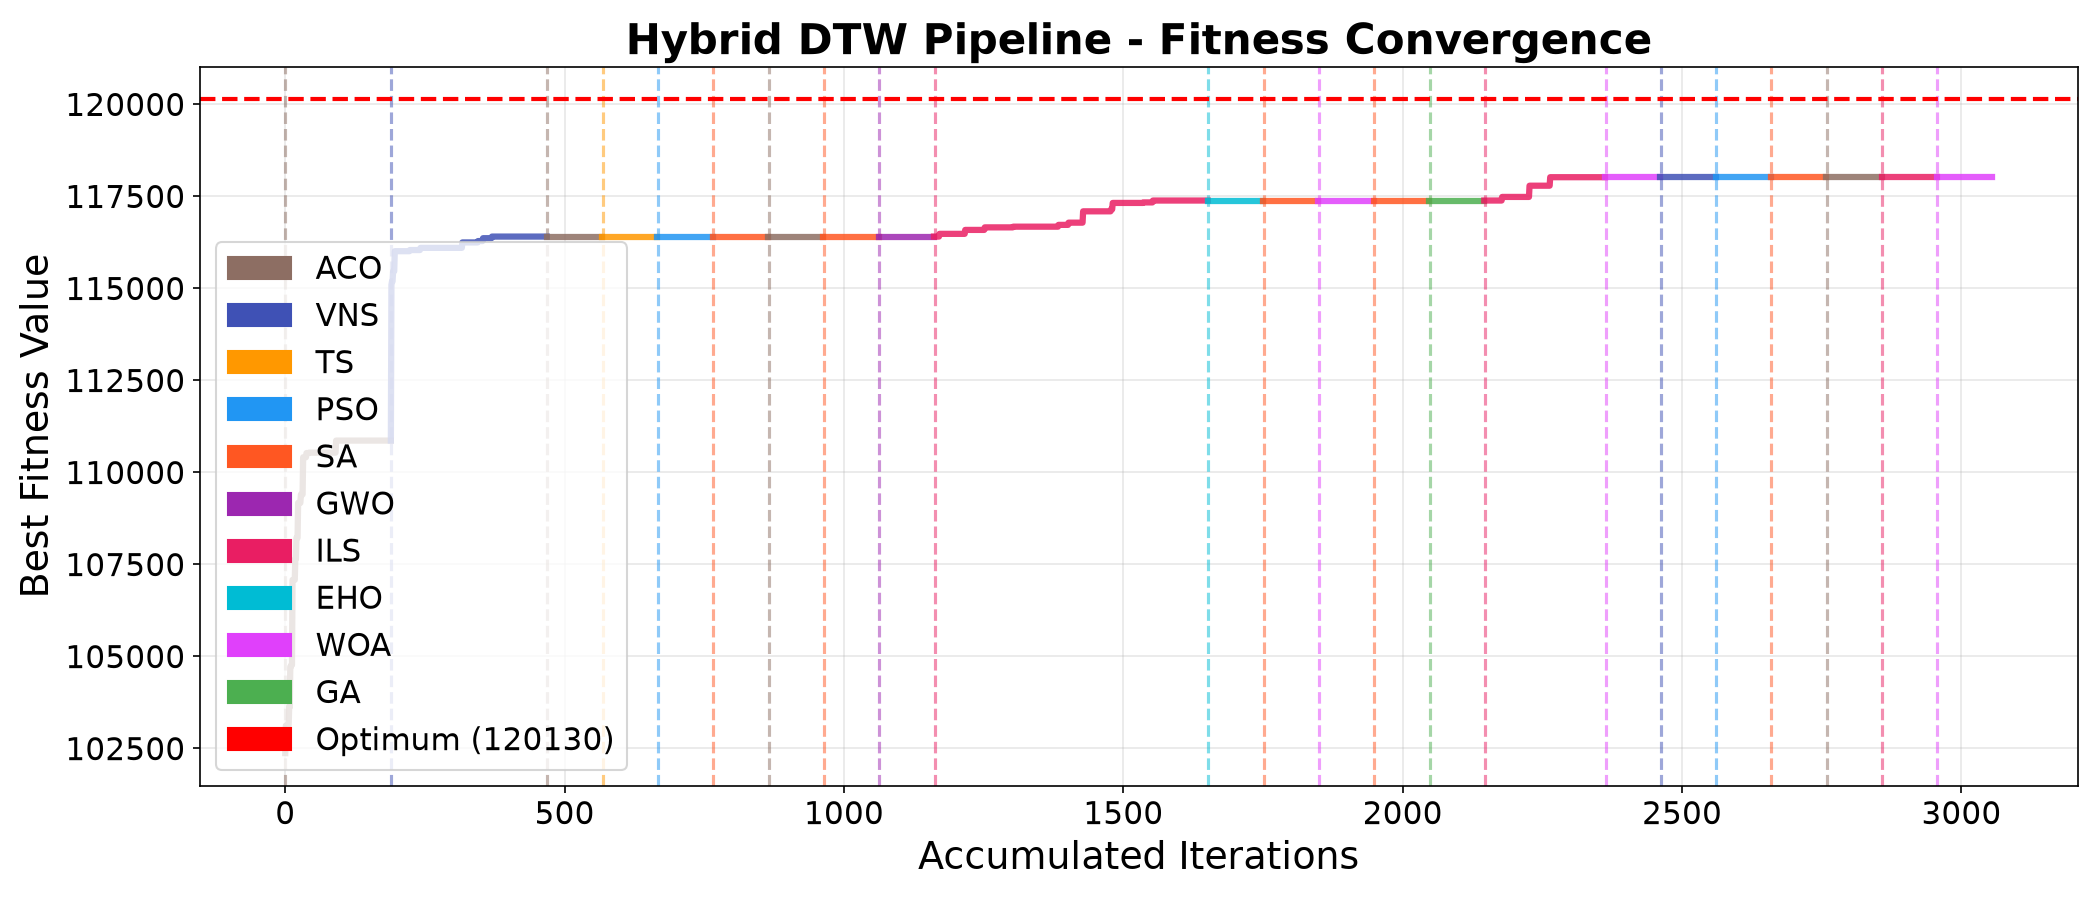
\includegraphics[width=0.32\textwidth]{imagenes_paper/mkp_dtw_3k_mknapcb3_convergencia.png}}\hfill
\subfloat[Elastic metric $\Delta=D_1-D_2$.]{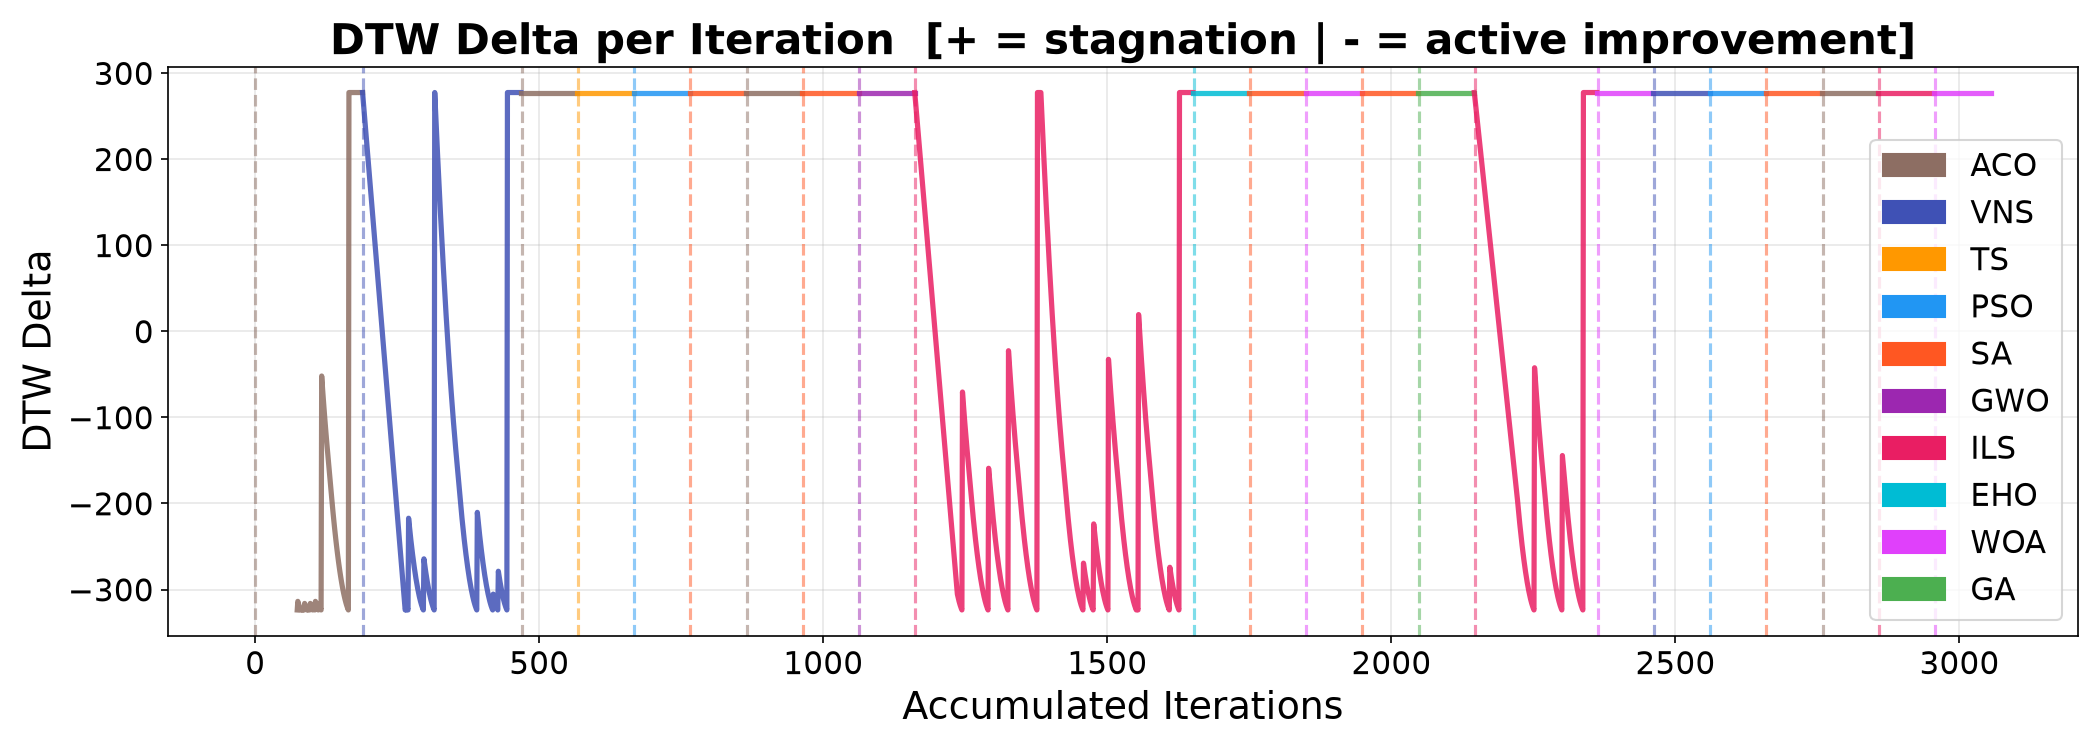
\includegraphics[width=0.32\textwidth]{imagenes_paper/mkp_dtw_3k_mknapcb3_delta.png}}
\caption{Diagnostic suite for instance \textbf{mknapcb3} ($n=500$, $m=5$) under the DTW framework with $T_{\max}=3{,}000$: (a)~final-fitness distribution over $N=31$ runs; (b)~convergence trajectory of the best run; (c)~elastic warping profile $\Delta$.}
\label{fig:mkp-best-cb3}
\end{figure}

% --- mknapcb4: DTW, 3,000 iterations ---
\begin{figure}[htbp]
\centering
\subfloat[Metaheuristic comparison.]{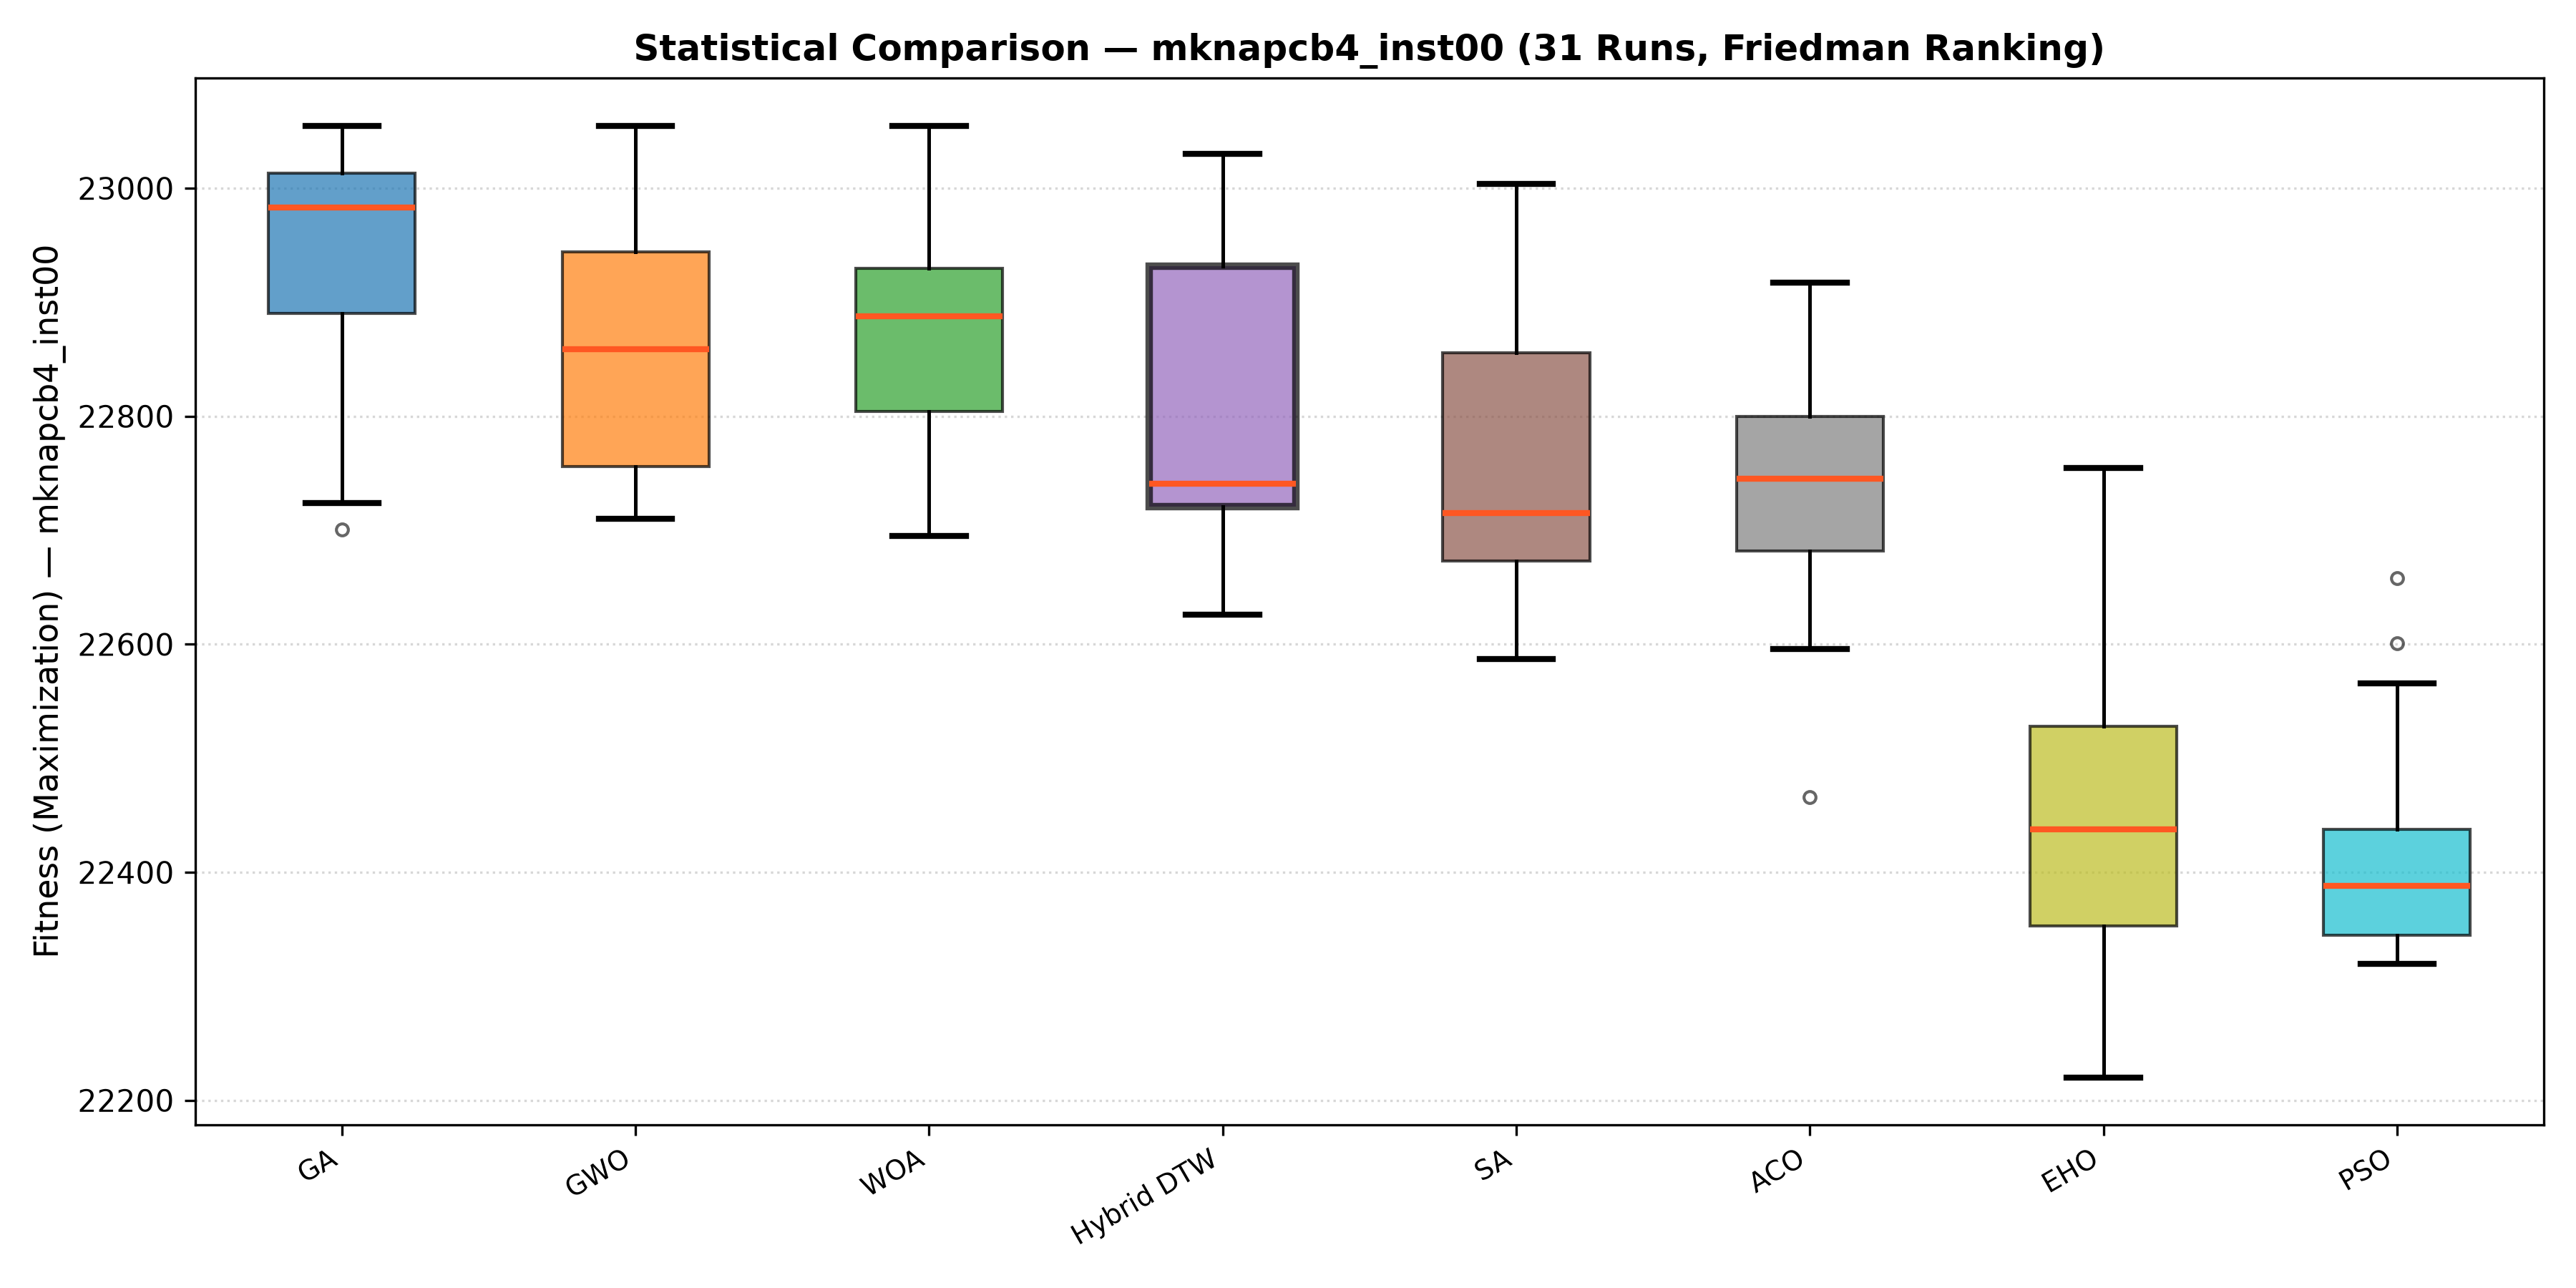
\includegraphics[width=0.32\textwidth]{imagenes_paper/mkp_dtw_3k_mknapcb4_comparativo_mh.png}}\hfill
\subfloat[Best-run convergence.]{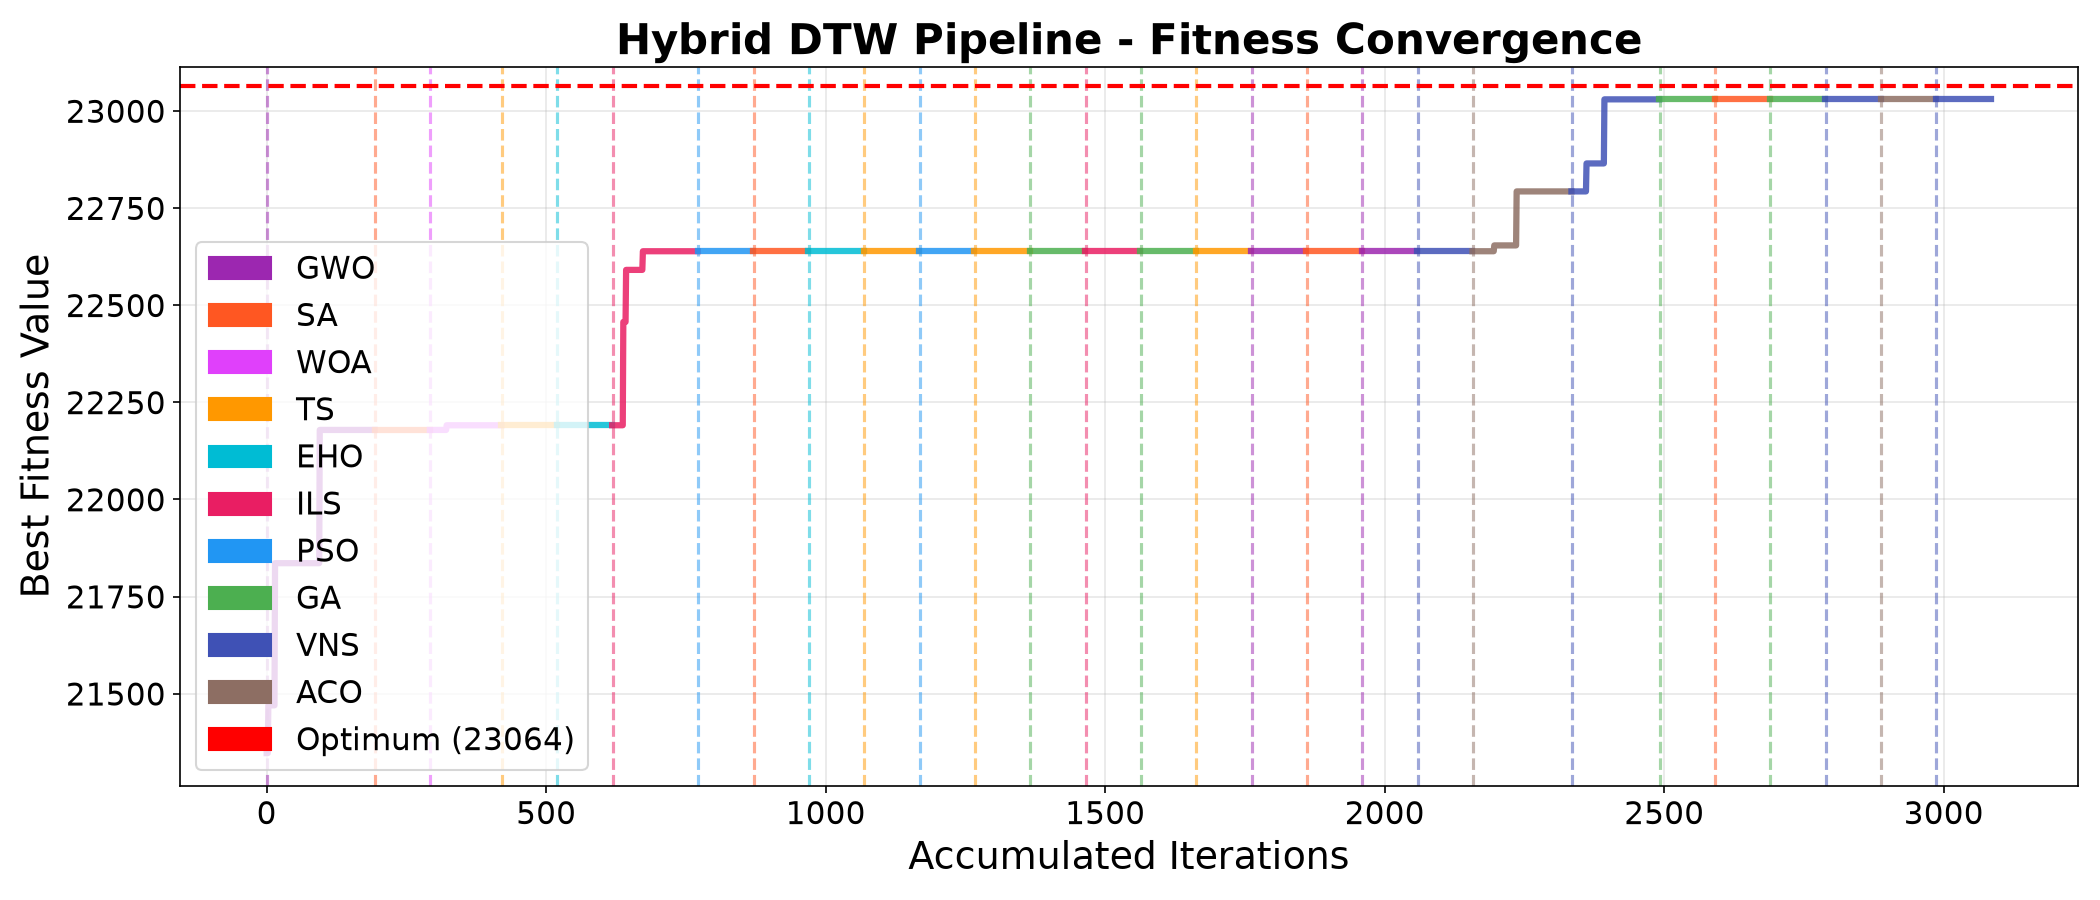
\includegraphics[width=0.32\textwidth]{imagenes_paper/mkp_dtw_3k_mknapcb4_convergencia.png}}\hfill
\subfloat[Elastic metric $\Delta=D_1-D_2$.]{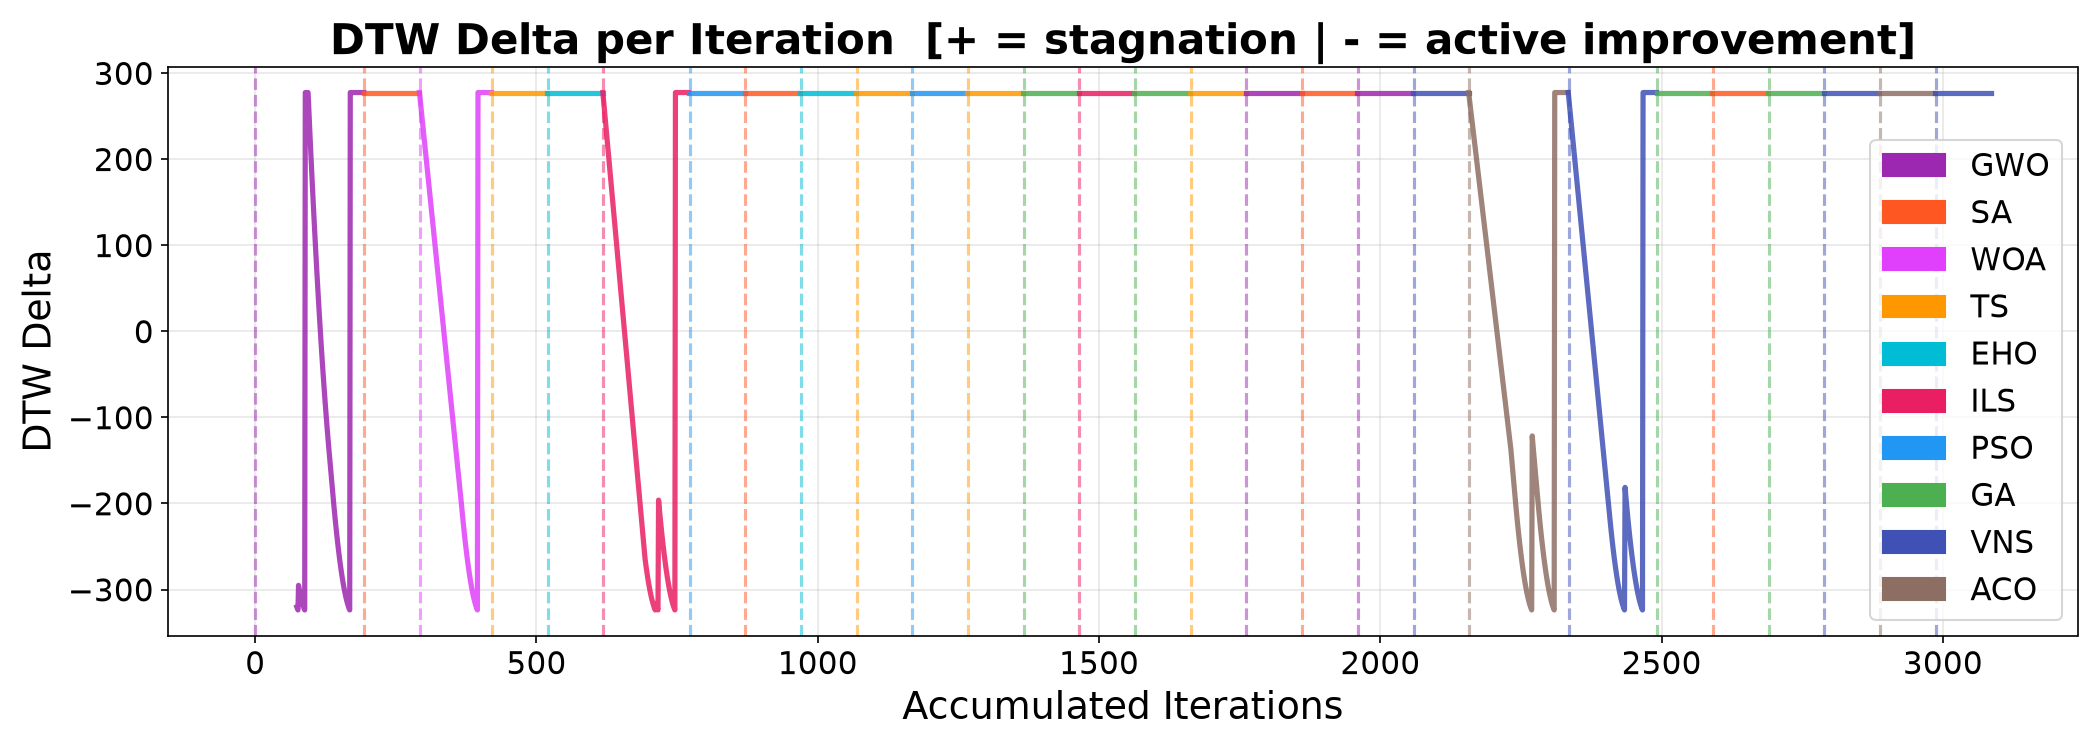
\includegraphics[width=0.32\textwidth]{imagenes_paper/mkp_dtw_3k_mknapcb4_delta.png}}
\caption{Diagnostic suite for instance \textbf{mknapcb4} ($n=100$, $m=10$) under the DTW framework with $T_{\max}=3{,}000$: (a)~final-fitness distribution over $N=31$ runs; (b)~convergence trajectory of the best run; (c)~elastic warping profile $\Delta$.}
\label{fig:mkp-best-cb4}
\end{figure}

% --- mknapcb5: DTW, 3,000 iterations ---
\begin{figure}[htbp]
\centering
\subfloat[Metaheuristic comparison.]{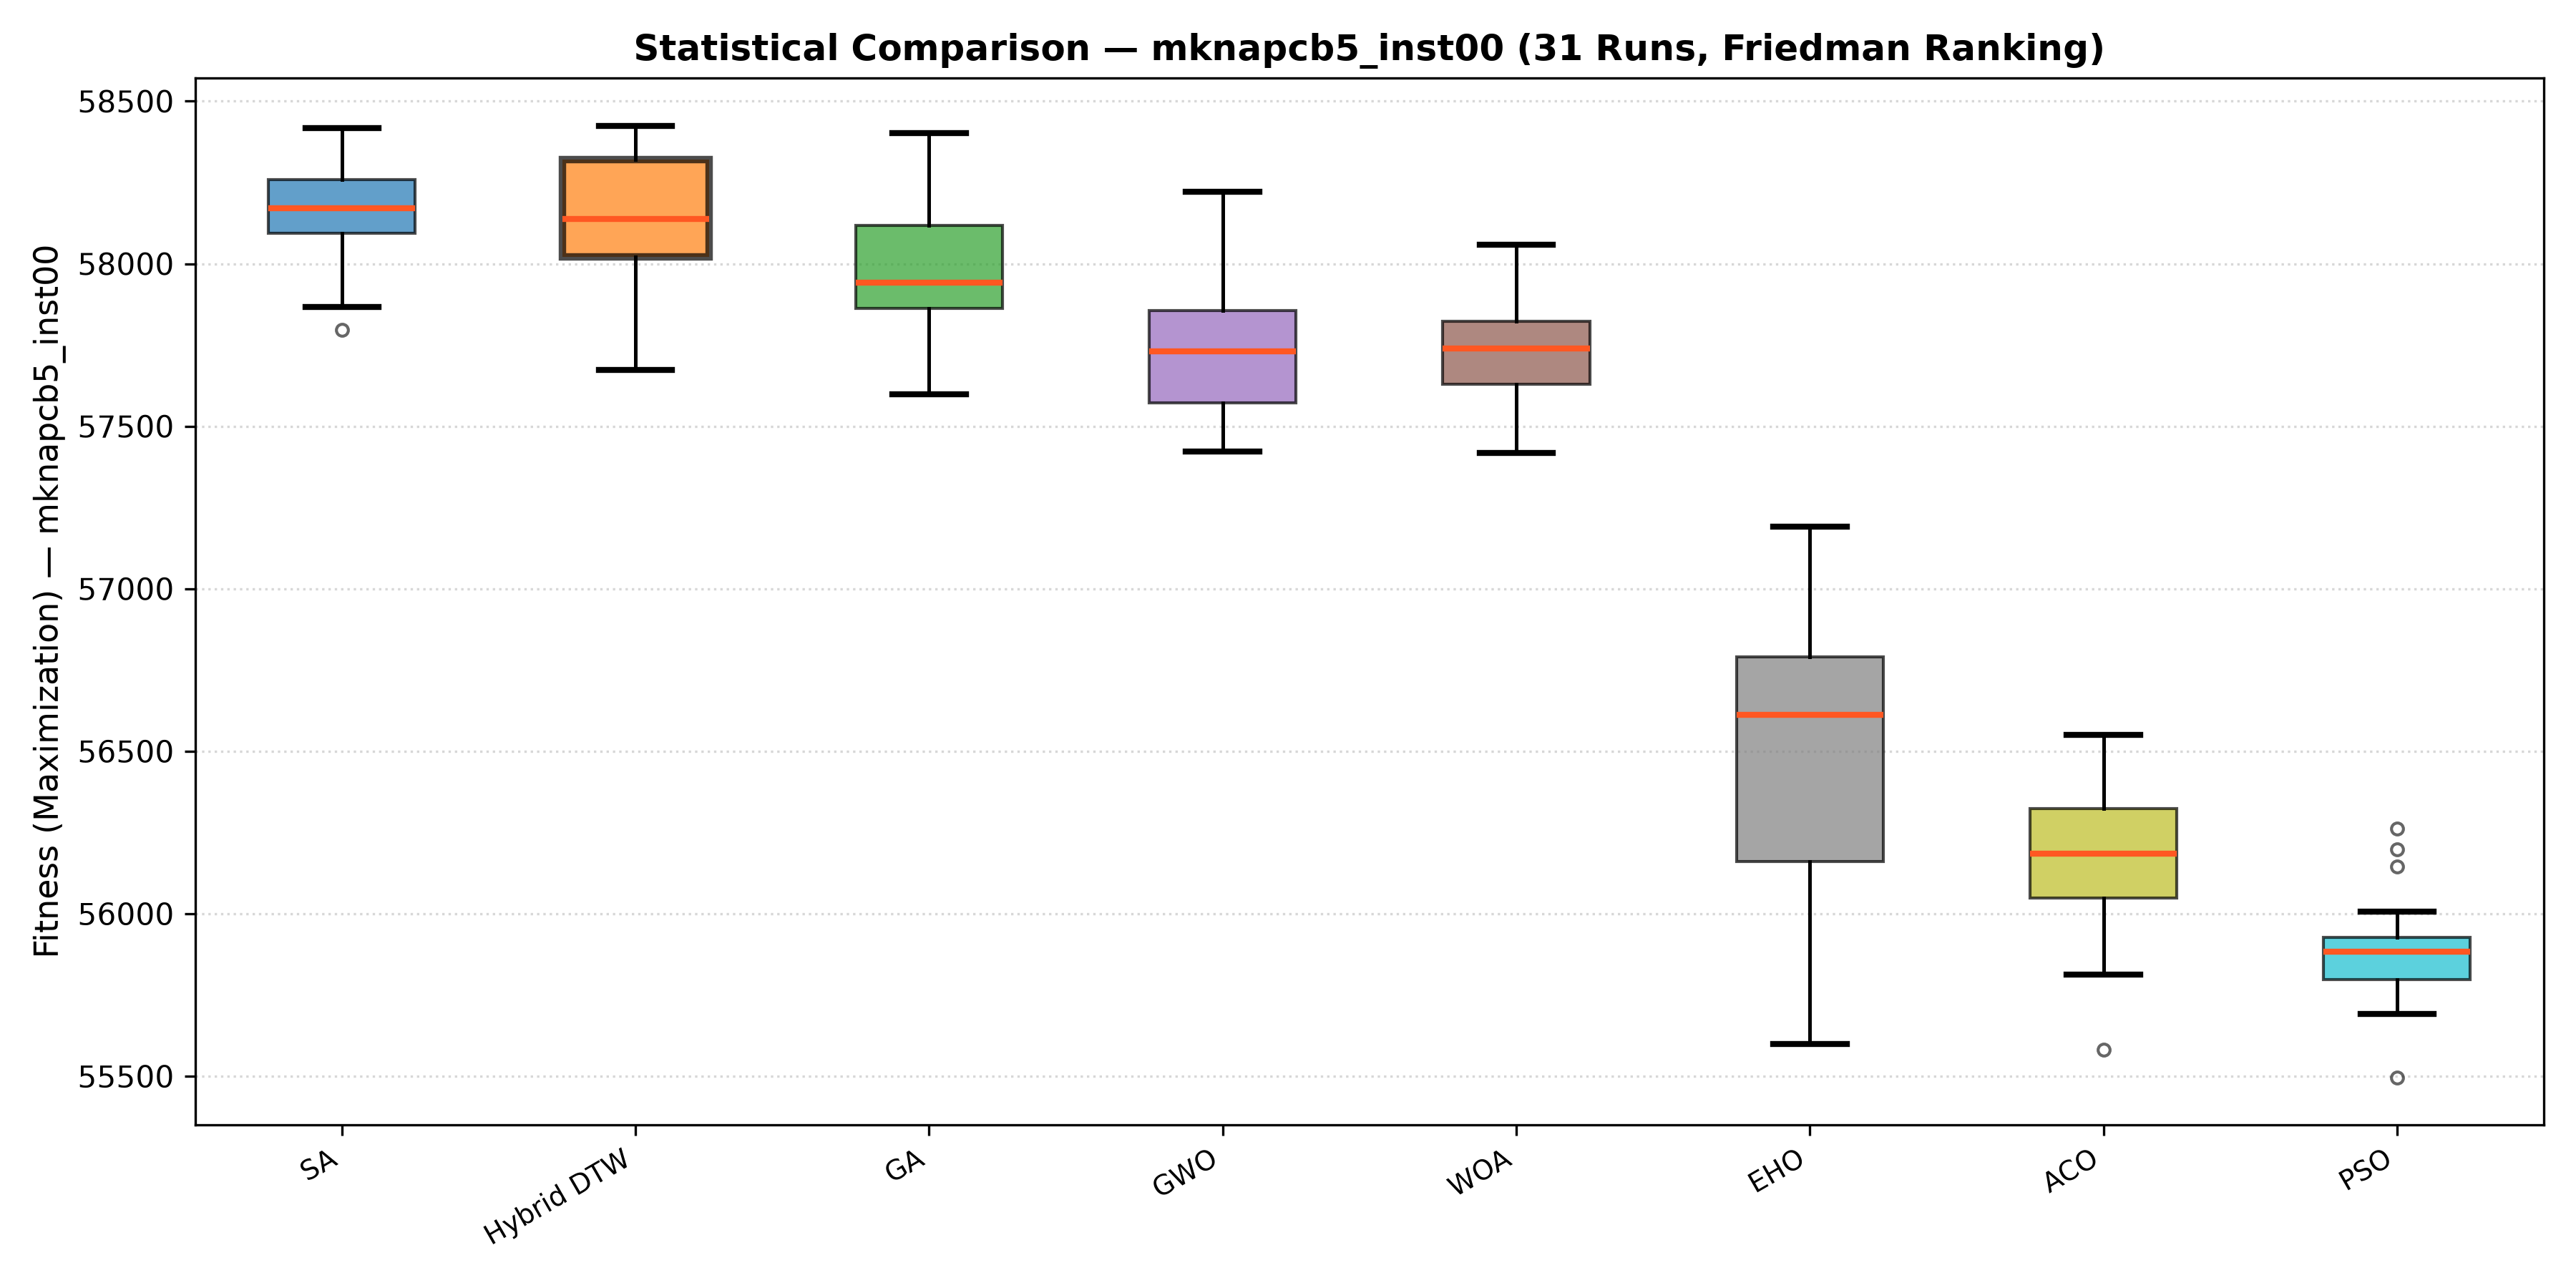
\includegraphics[width=0.32\textwidth]{imagenes_paper/mkp_dtw_3k_mknapcb5_comparativo_mh.png}}\hfill
\subfloat[Best-run convergence.]{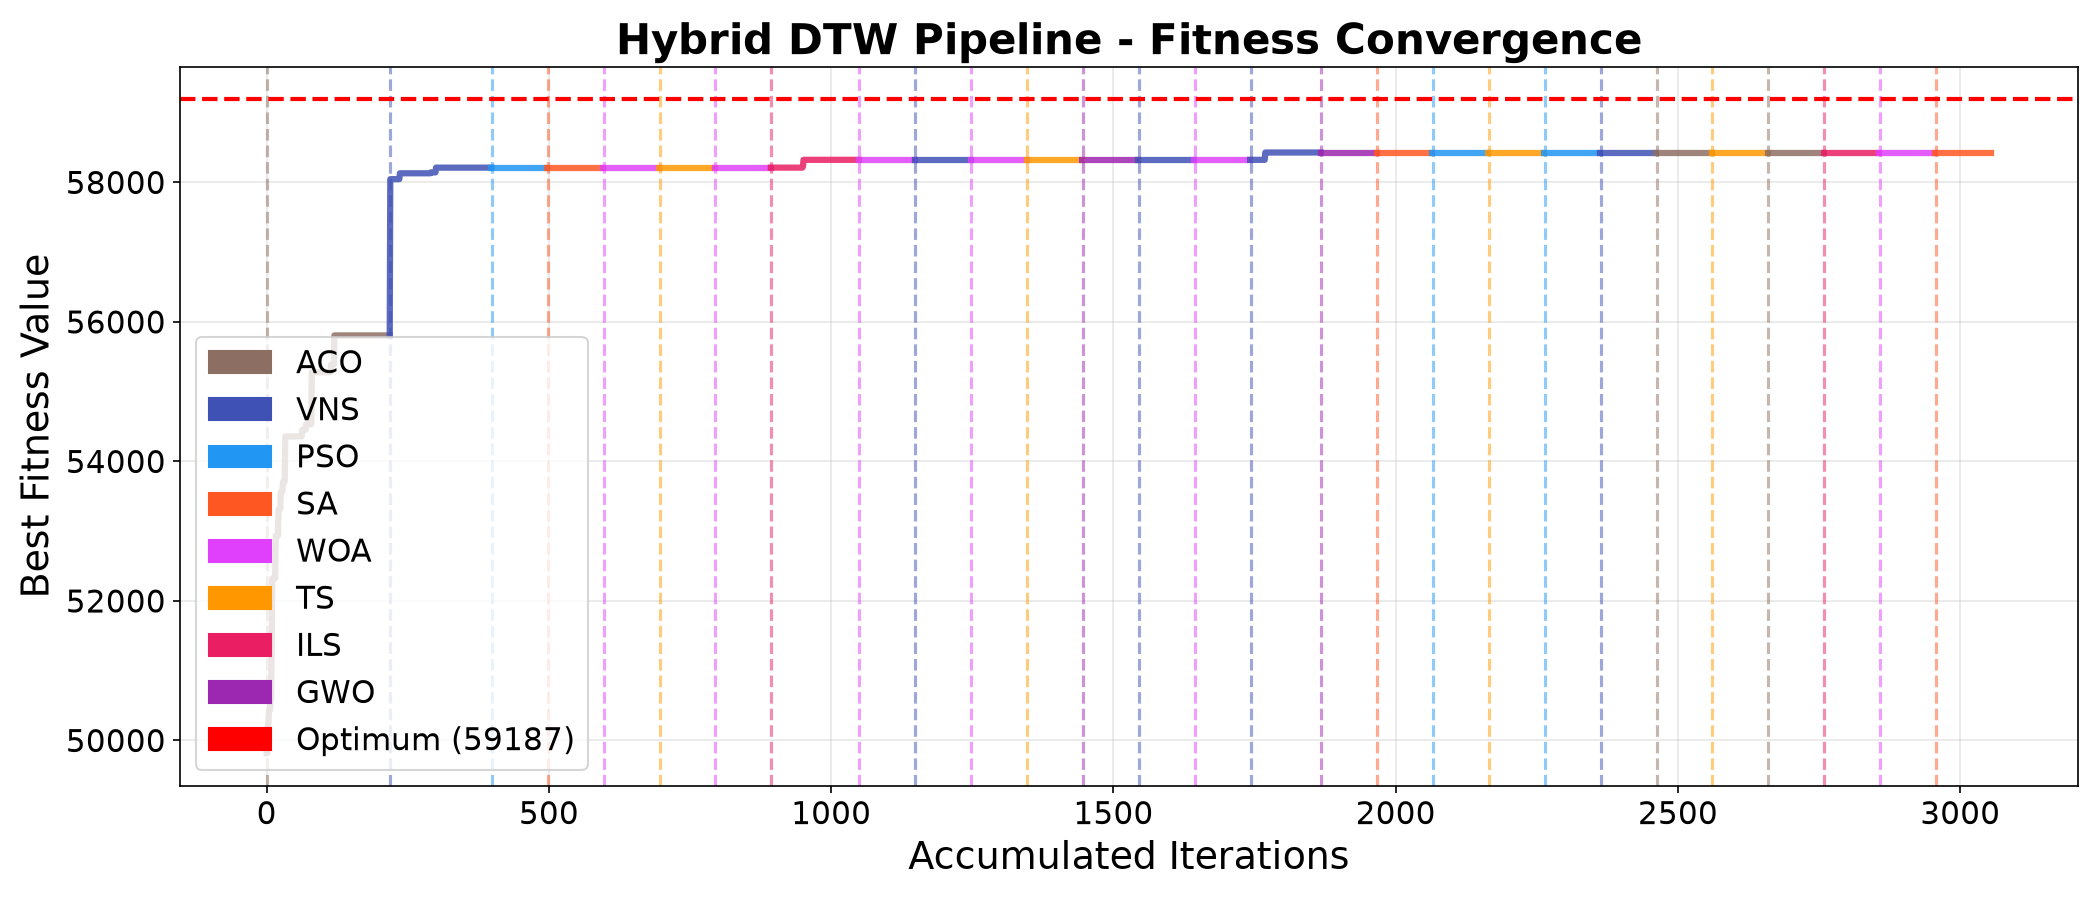
\includegraphics[width=0.32\textwidth]{imagenes_paper/mkp_dtw_3k_mknapcb5_convergencia.png}}\hfill
\subfloat[Elastic metric $\Delta=D_1-D_2$.]{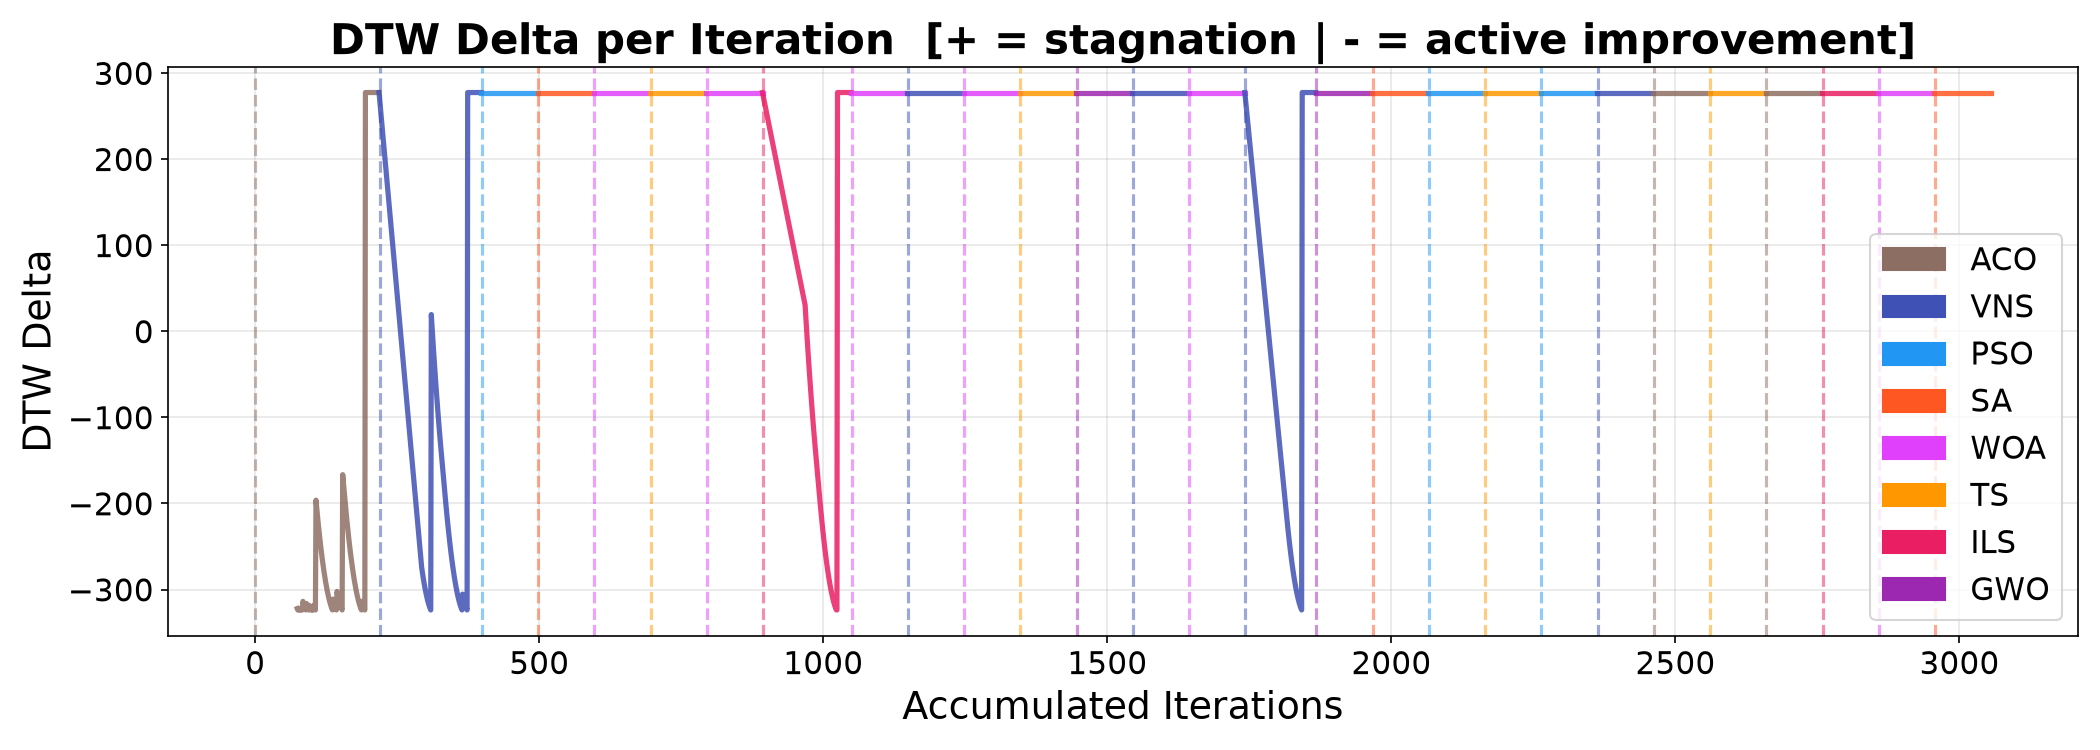
\includegraphics[width=0.32\textwidth]{imagenes_paper/mkp_dtw_3k_mknapcb5_delta.png}}
\caption{Diagnostic suite for instance \textbf{mknapcb5} ($n=250$, $m=10$) under the DTW framework with $T_{\max}=3{,}000$: (a)~final-fitness distribution over $N=31$ runs; (b)~convergence trajectory of the best run; (c)~elastic warping profile $\Delta$.}
\label{fig:mkp-best-cb5}
\end{figure}

% --- mknapcb6: DTW, 3,000 iterations ---
\begin{figure}[htbp]
\centering
\subfloat[Metaheuristic comparison.]{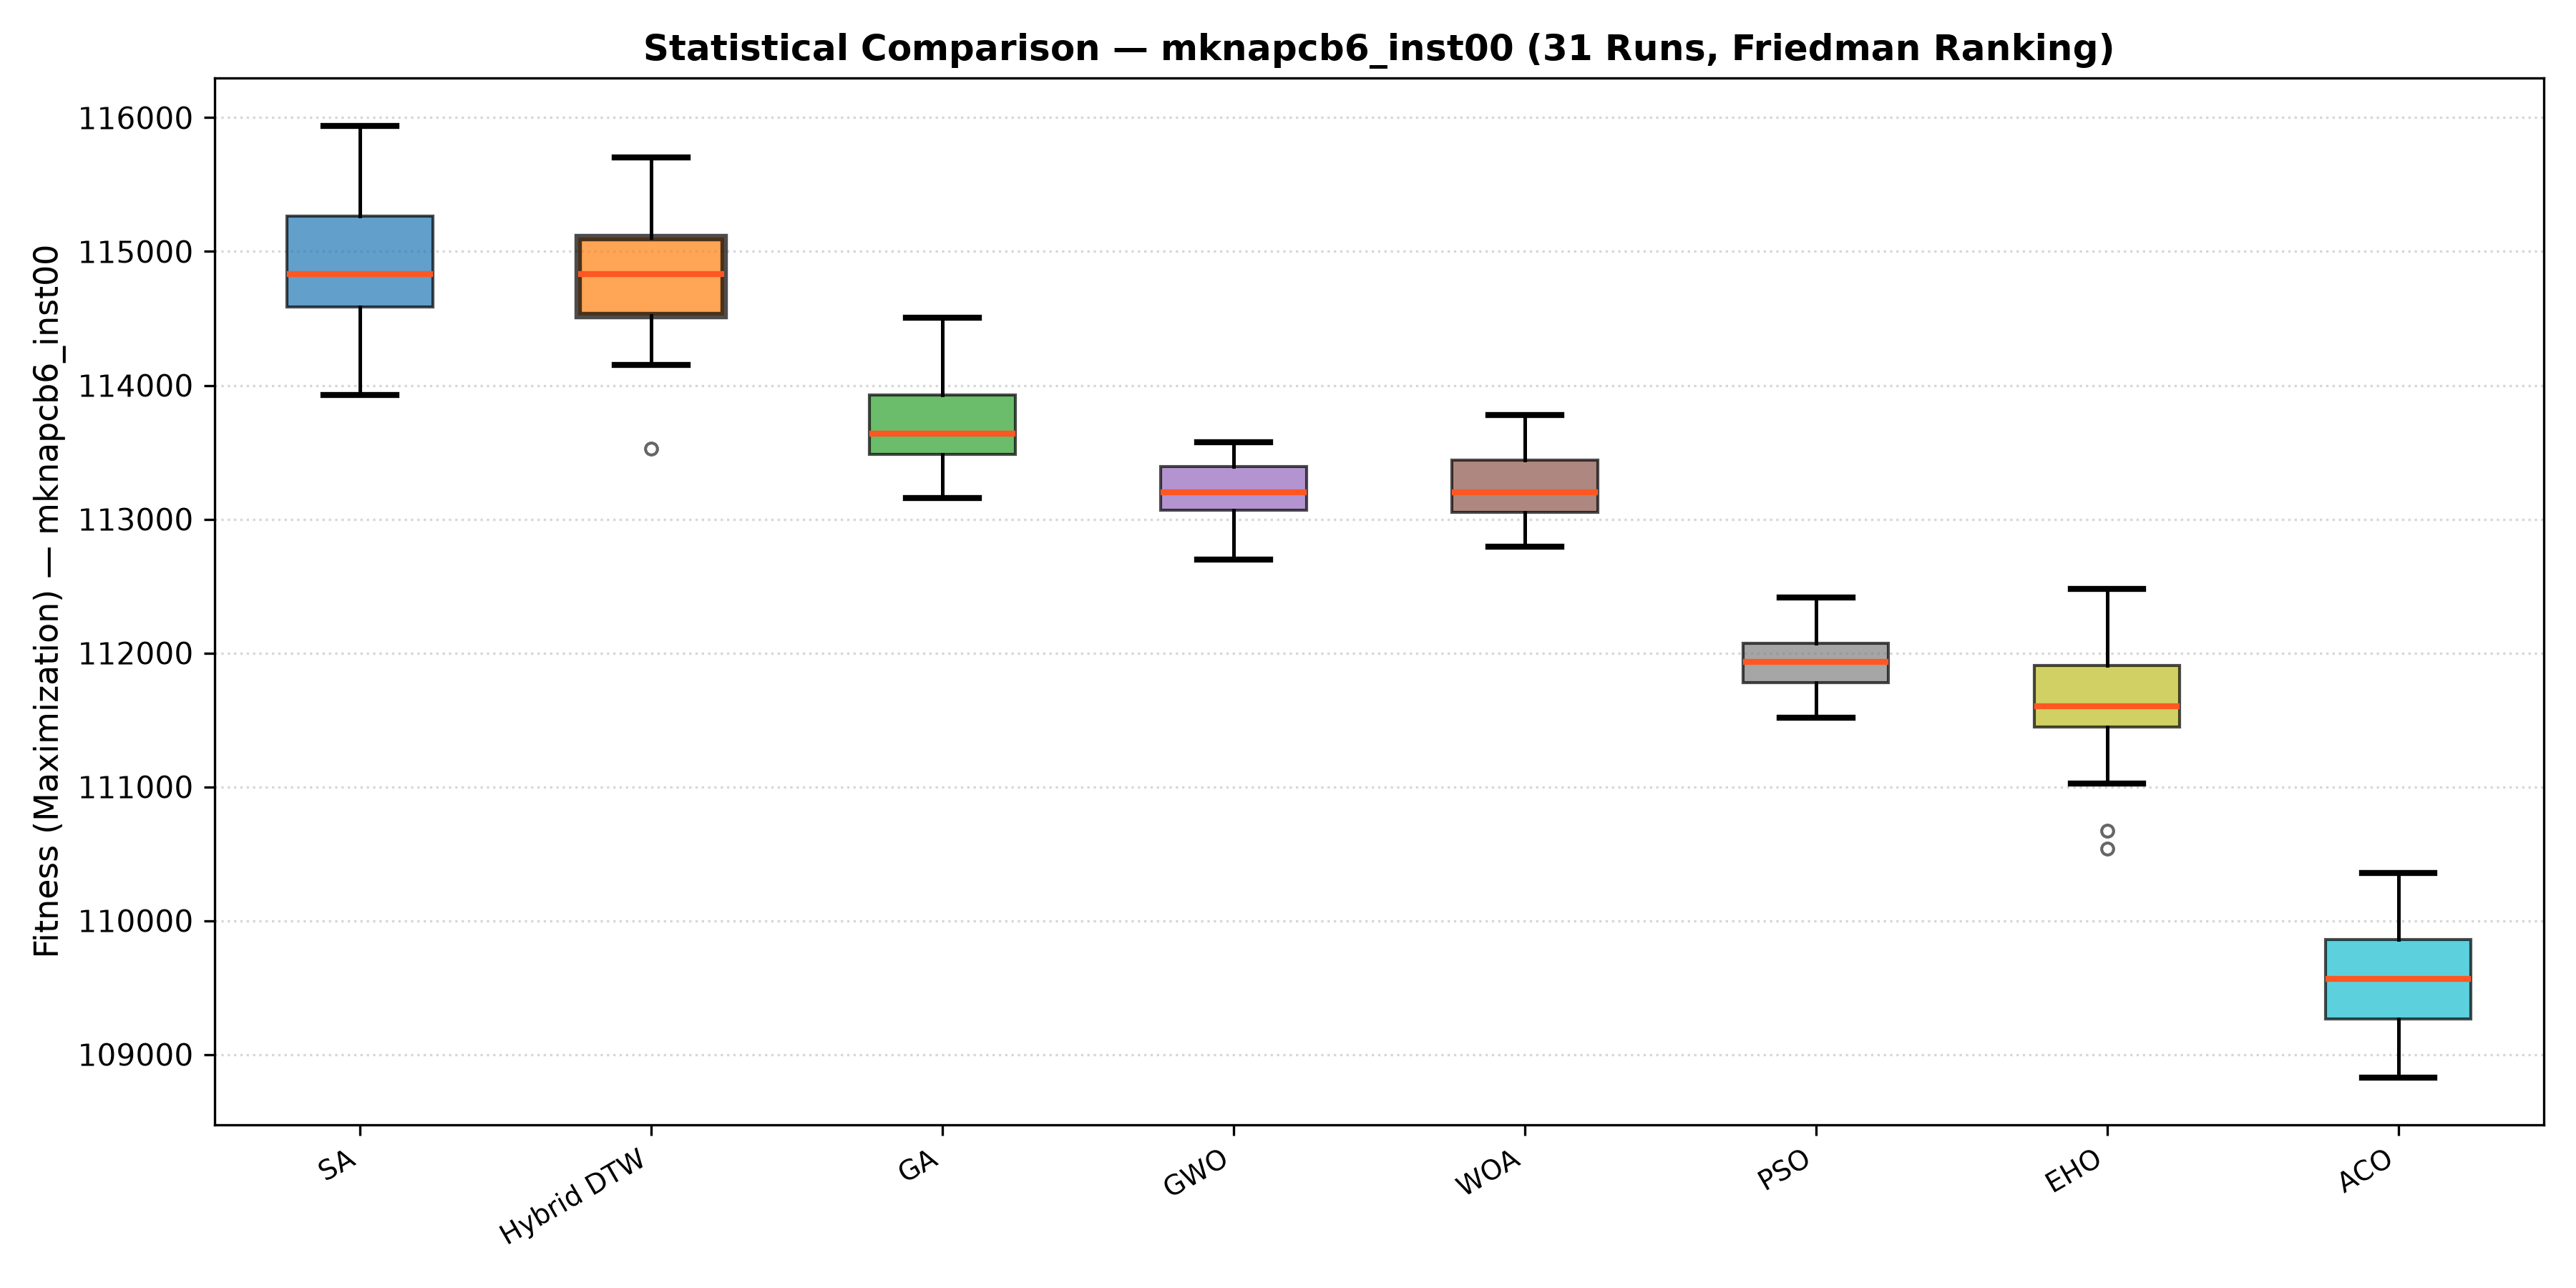
\includegraphics[width=0.32\textwidth]{imagenes_paper/mkp_dtw_3k_mknapcb6_comparativo_mh.png}}\hfill
\subfloat[Best-run convergence.]{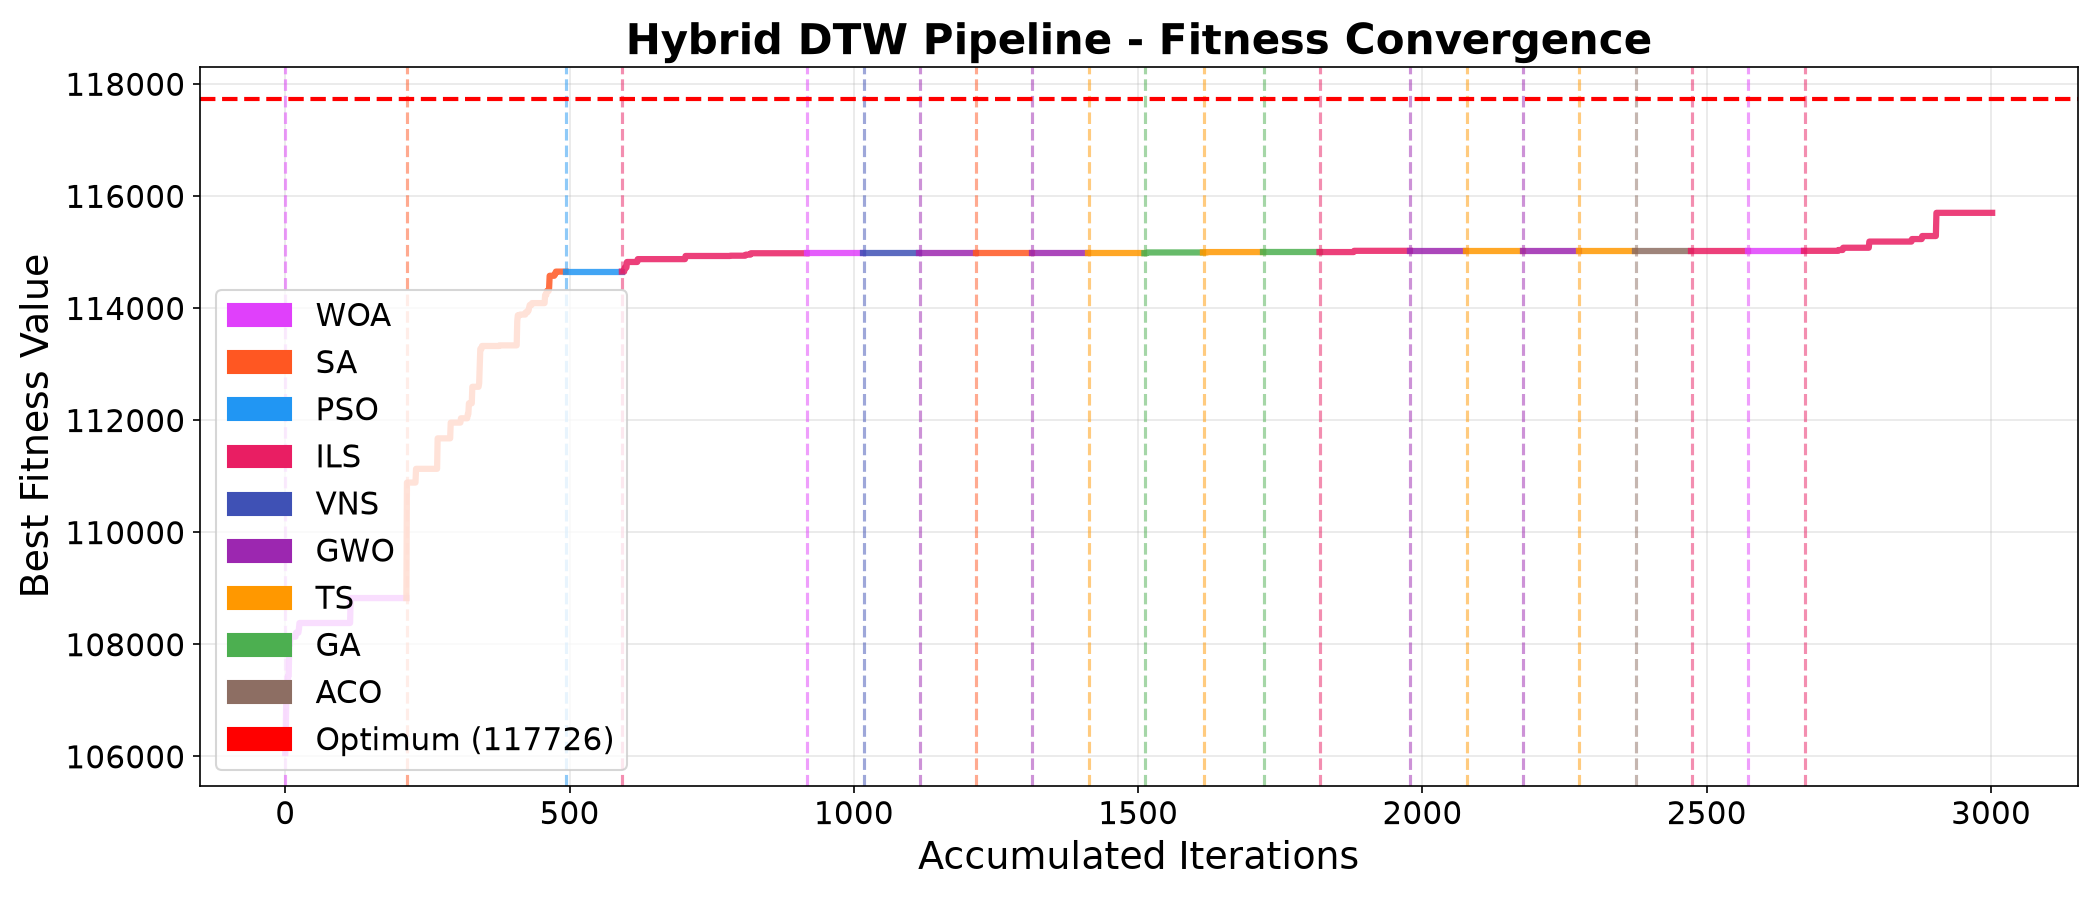
\includegraphics[width=0.32\textwidth]{imagenes_paper/mkp_dtw_3k_mknapcb6_convergencia.png}}\hfill
\subfloat[Elastic metric $\Delta=D_1-D_2$.]{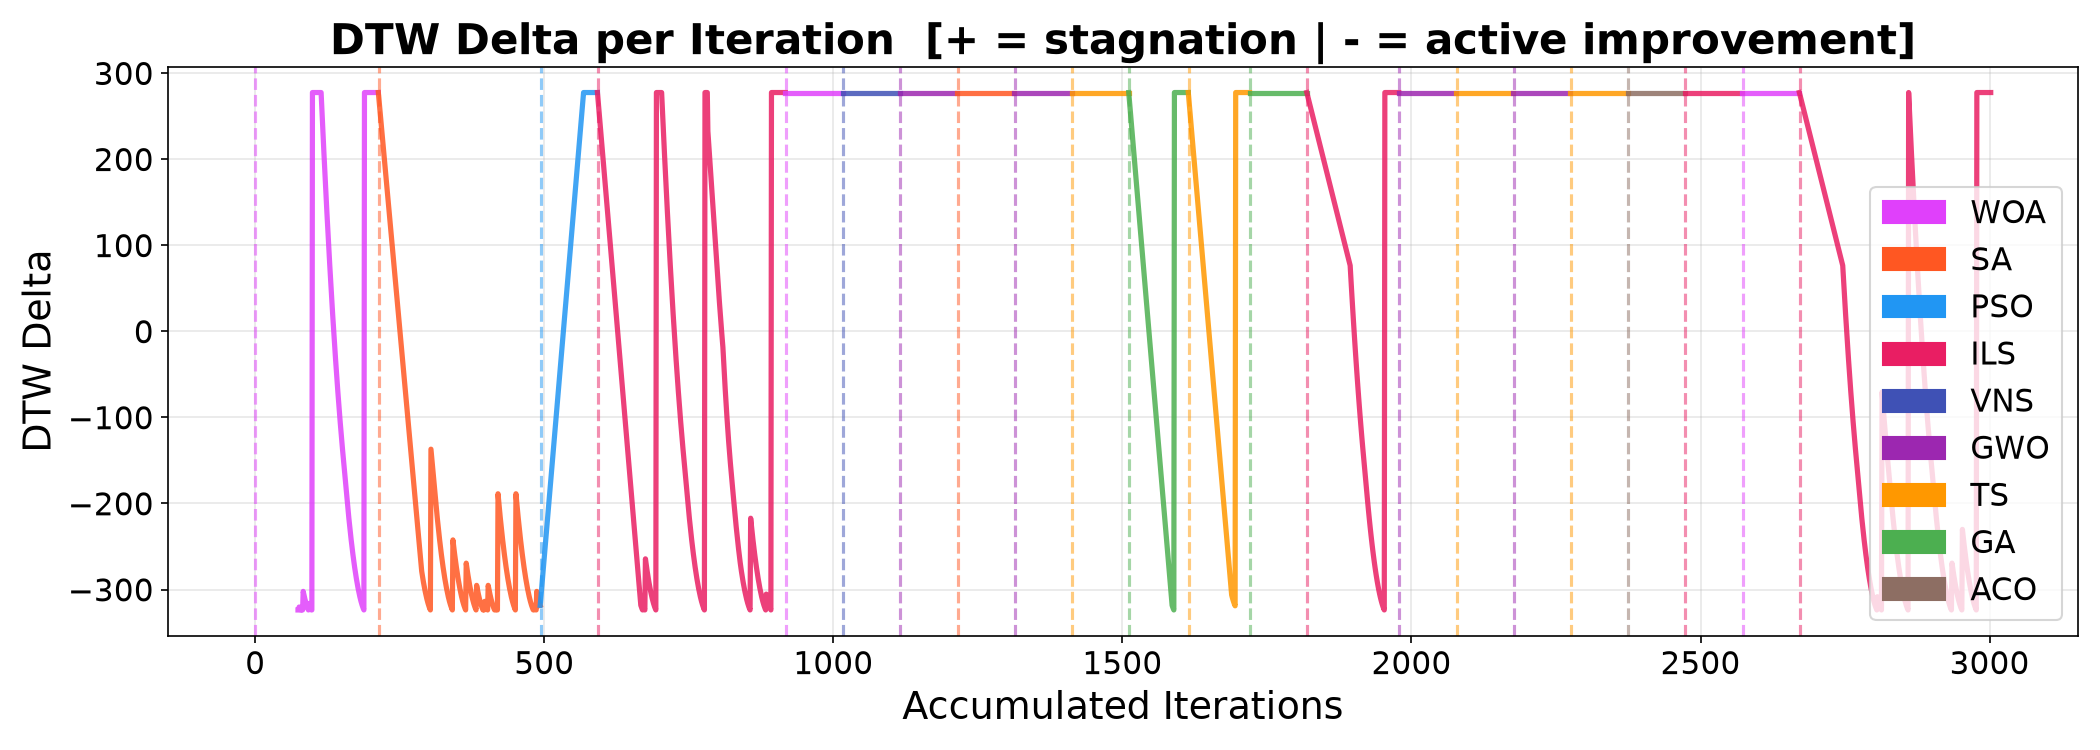
\includegraphics[width=0.32\textwidth]{imagenes_paper/mkp_dtw_3k_mknapcb6_delta.png}}
\caption{Diagnostic suite for instance \textbf{mknapcb6} ($n=500$, $m=10$) under the DTW framework with $T_{\max}=3{,}000$: (a)~final-fitness distribution over $N=31$ runs; (b)~convergence trajectory of the best run; (c)~elastic warping profile $\Delta$.}
\label{fig:mkp-best-cb6}
\end{figure}

% --- mknapcb7: DTW, 3,000 iterations ---
\begin{figure}[htbp]
\centering
\subfloat[Metaheuristic comparison.]{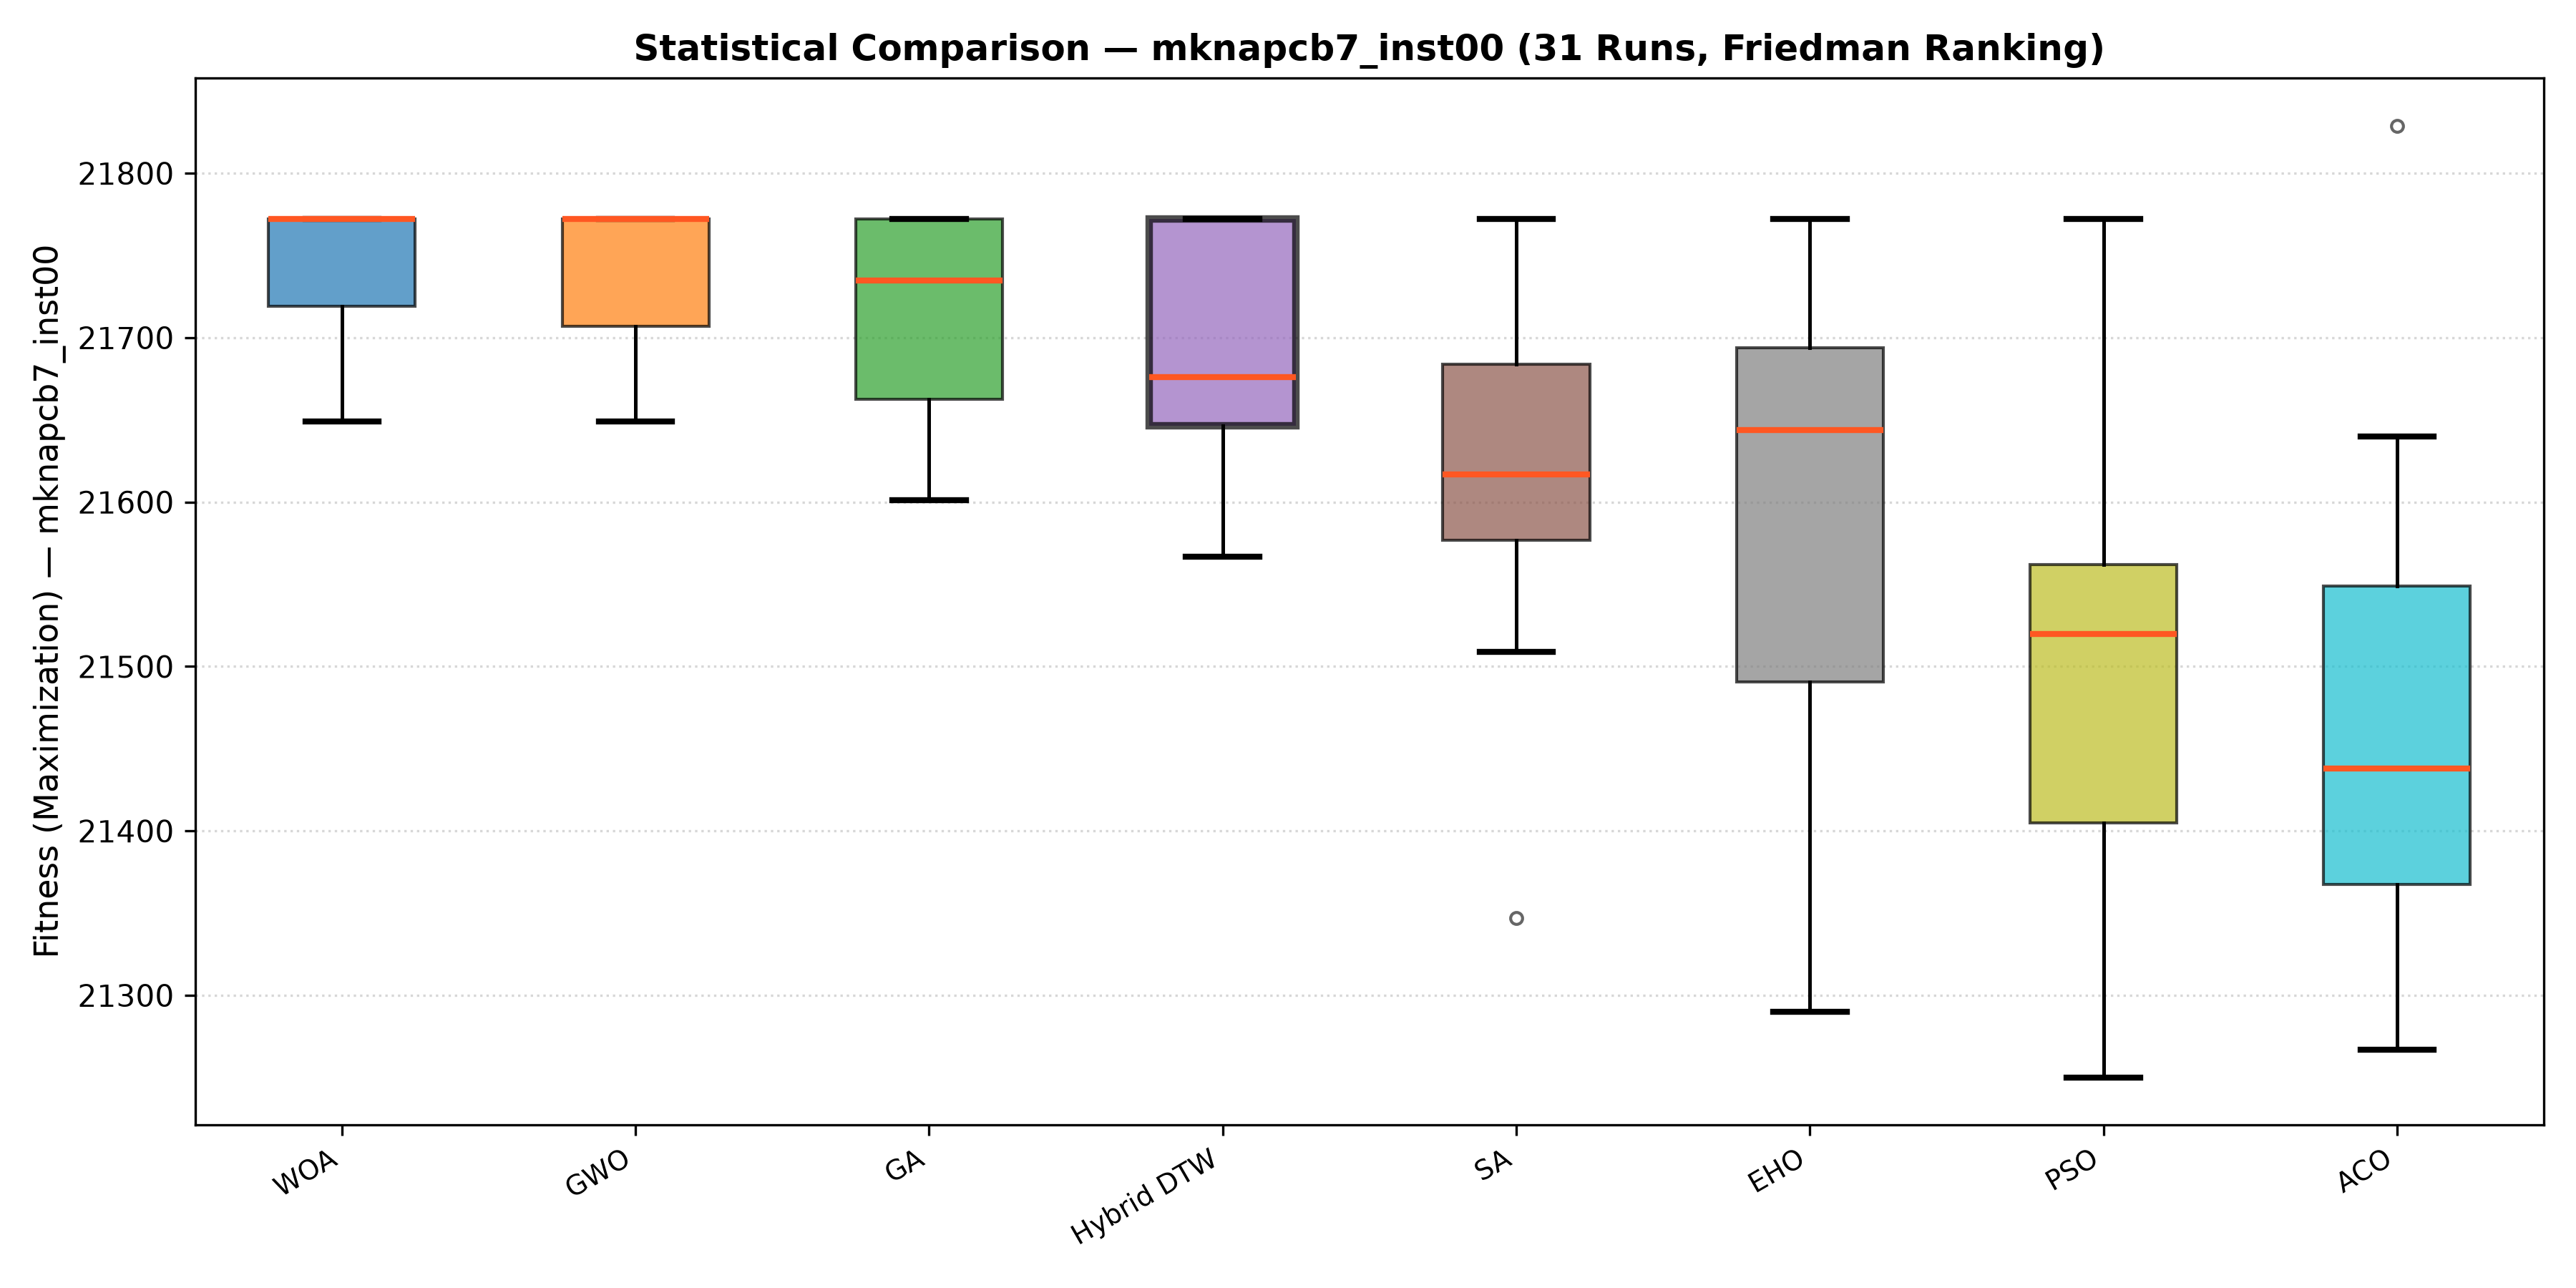
\includegraphics[width=0.32\textwidth]{imagenes_paper/mkp_dtw_3k_mknapcb7_comparativo_mh.png}}\hfill
\subfloat[Best-run convergence.]{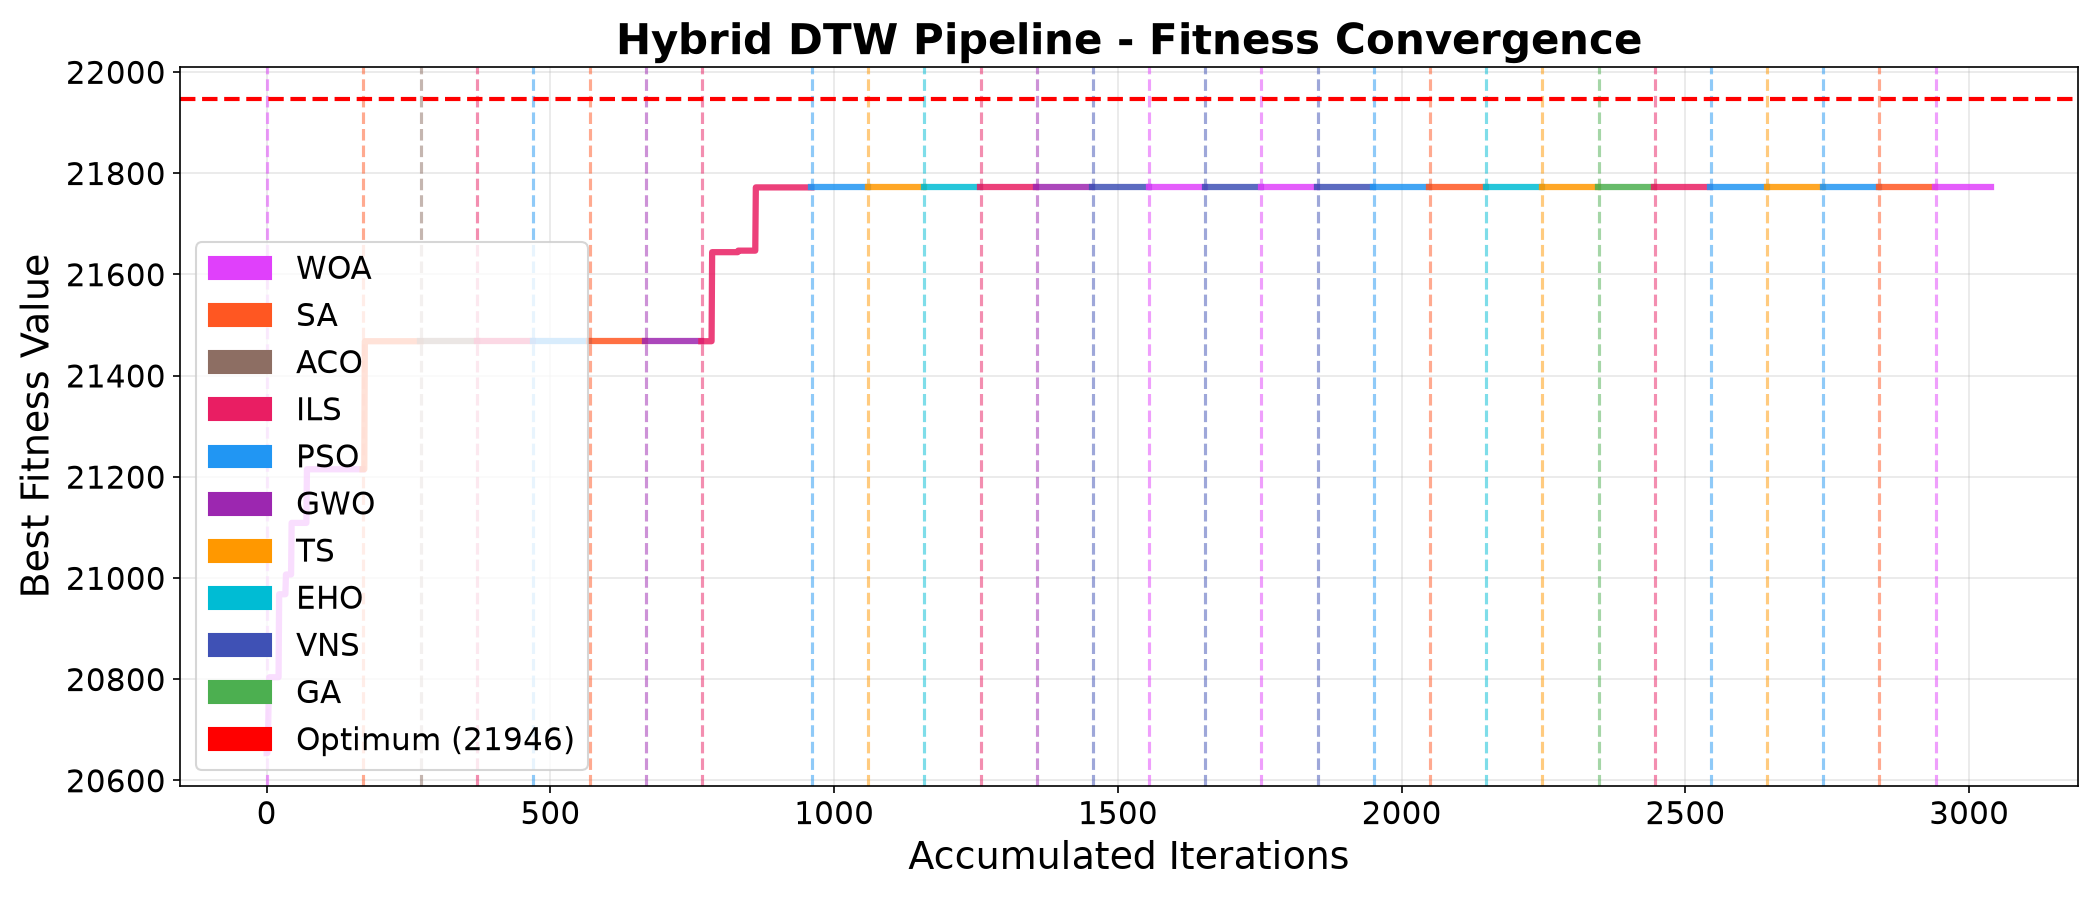
\includegraphics[width=0.32\textwidth]{imagenes_paper/mkp_dtw_3k_mknapcb7_convergencia.png}}\hfill
\subfloat[Elastic metric $\Delta=D_1-D_2$.]{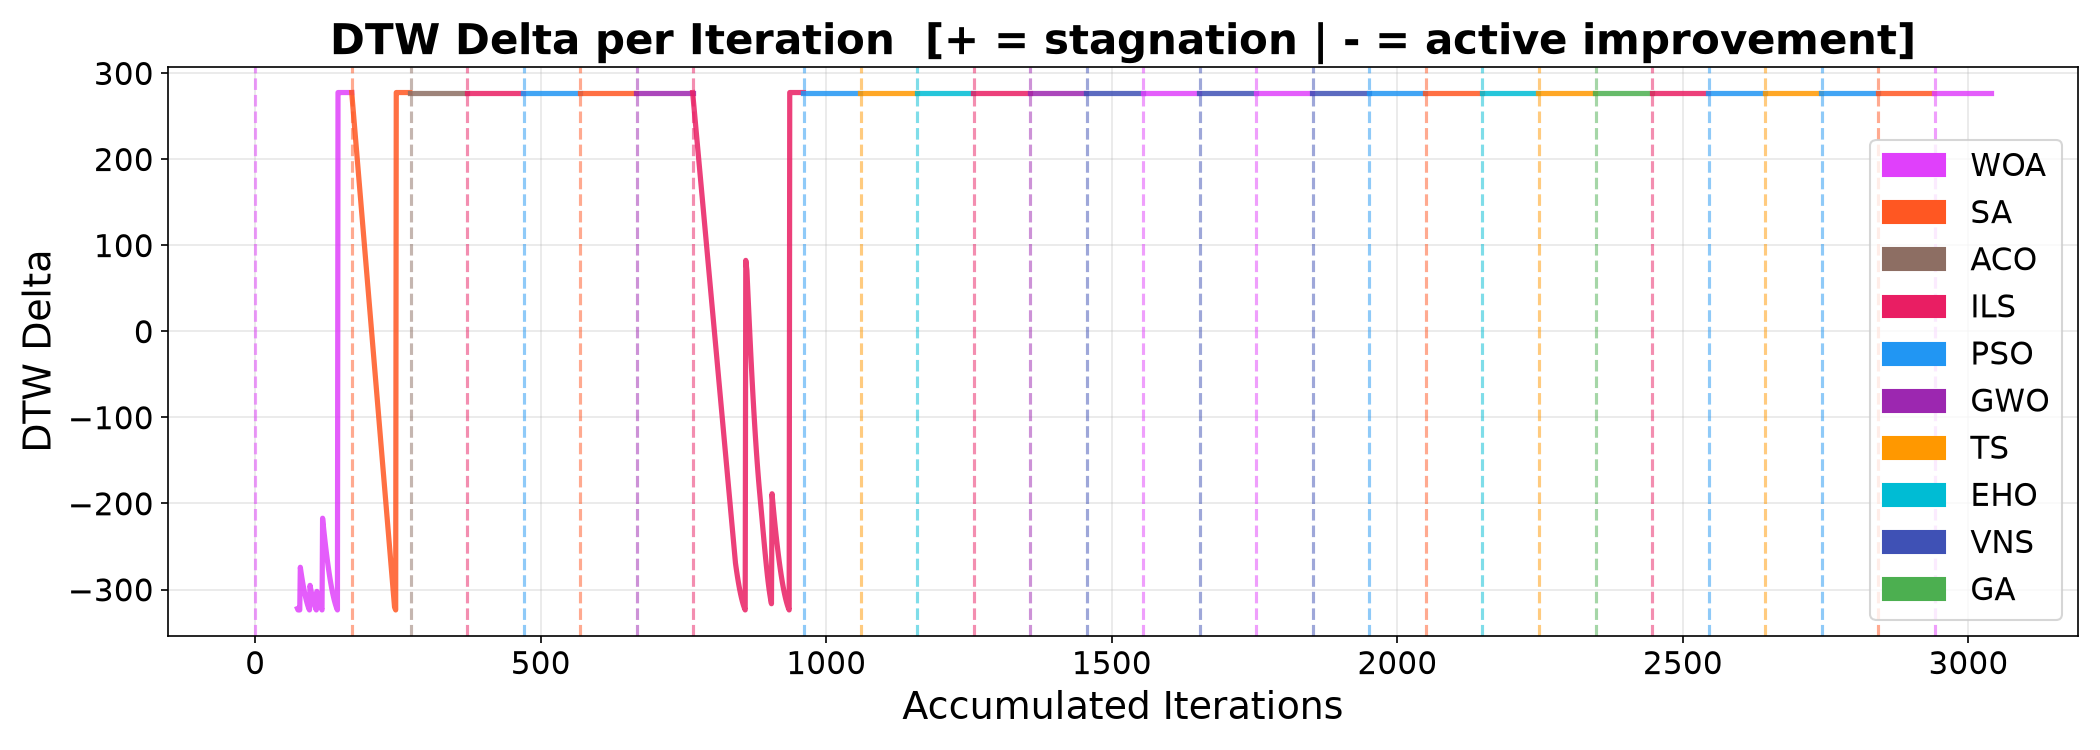
\includegraphics[width=0.32\textwidth]{imagenes_paper/mkp_dtw_3k_mknapcb7_delta.png}}
\caption{Diagnostic suite for instance \textbf{mknapcb7} ($n=100$, $m=30$) under the DTW framework with $T_{\max}=3{,}000$: (a)~final-fitness distribution over $N=31$ runs; (b)~convergence trajectory of the best run; (c)~elastic warping profile $\Delta$.}
\label{fig:mkp-best-cb7}
\end{figure}

% --- mknapcb8: DTW, 3,000 iterations ---
\begin{figure}[htbp]
\centering
\subfloat[Metaheuristic comparison.]{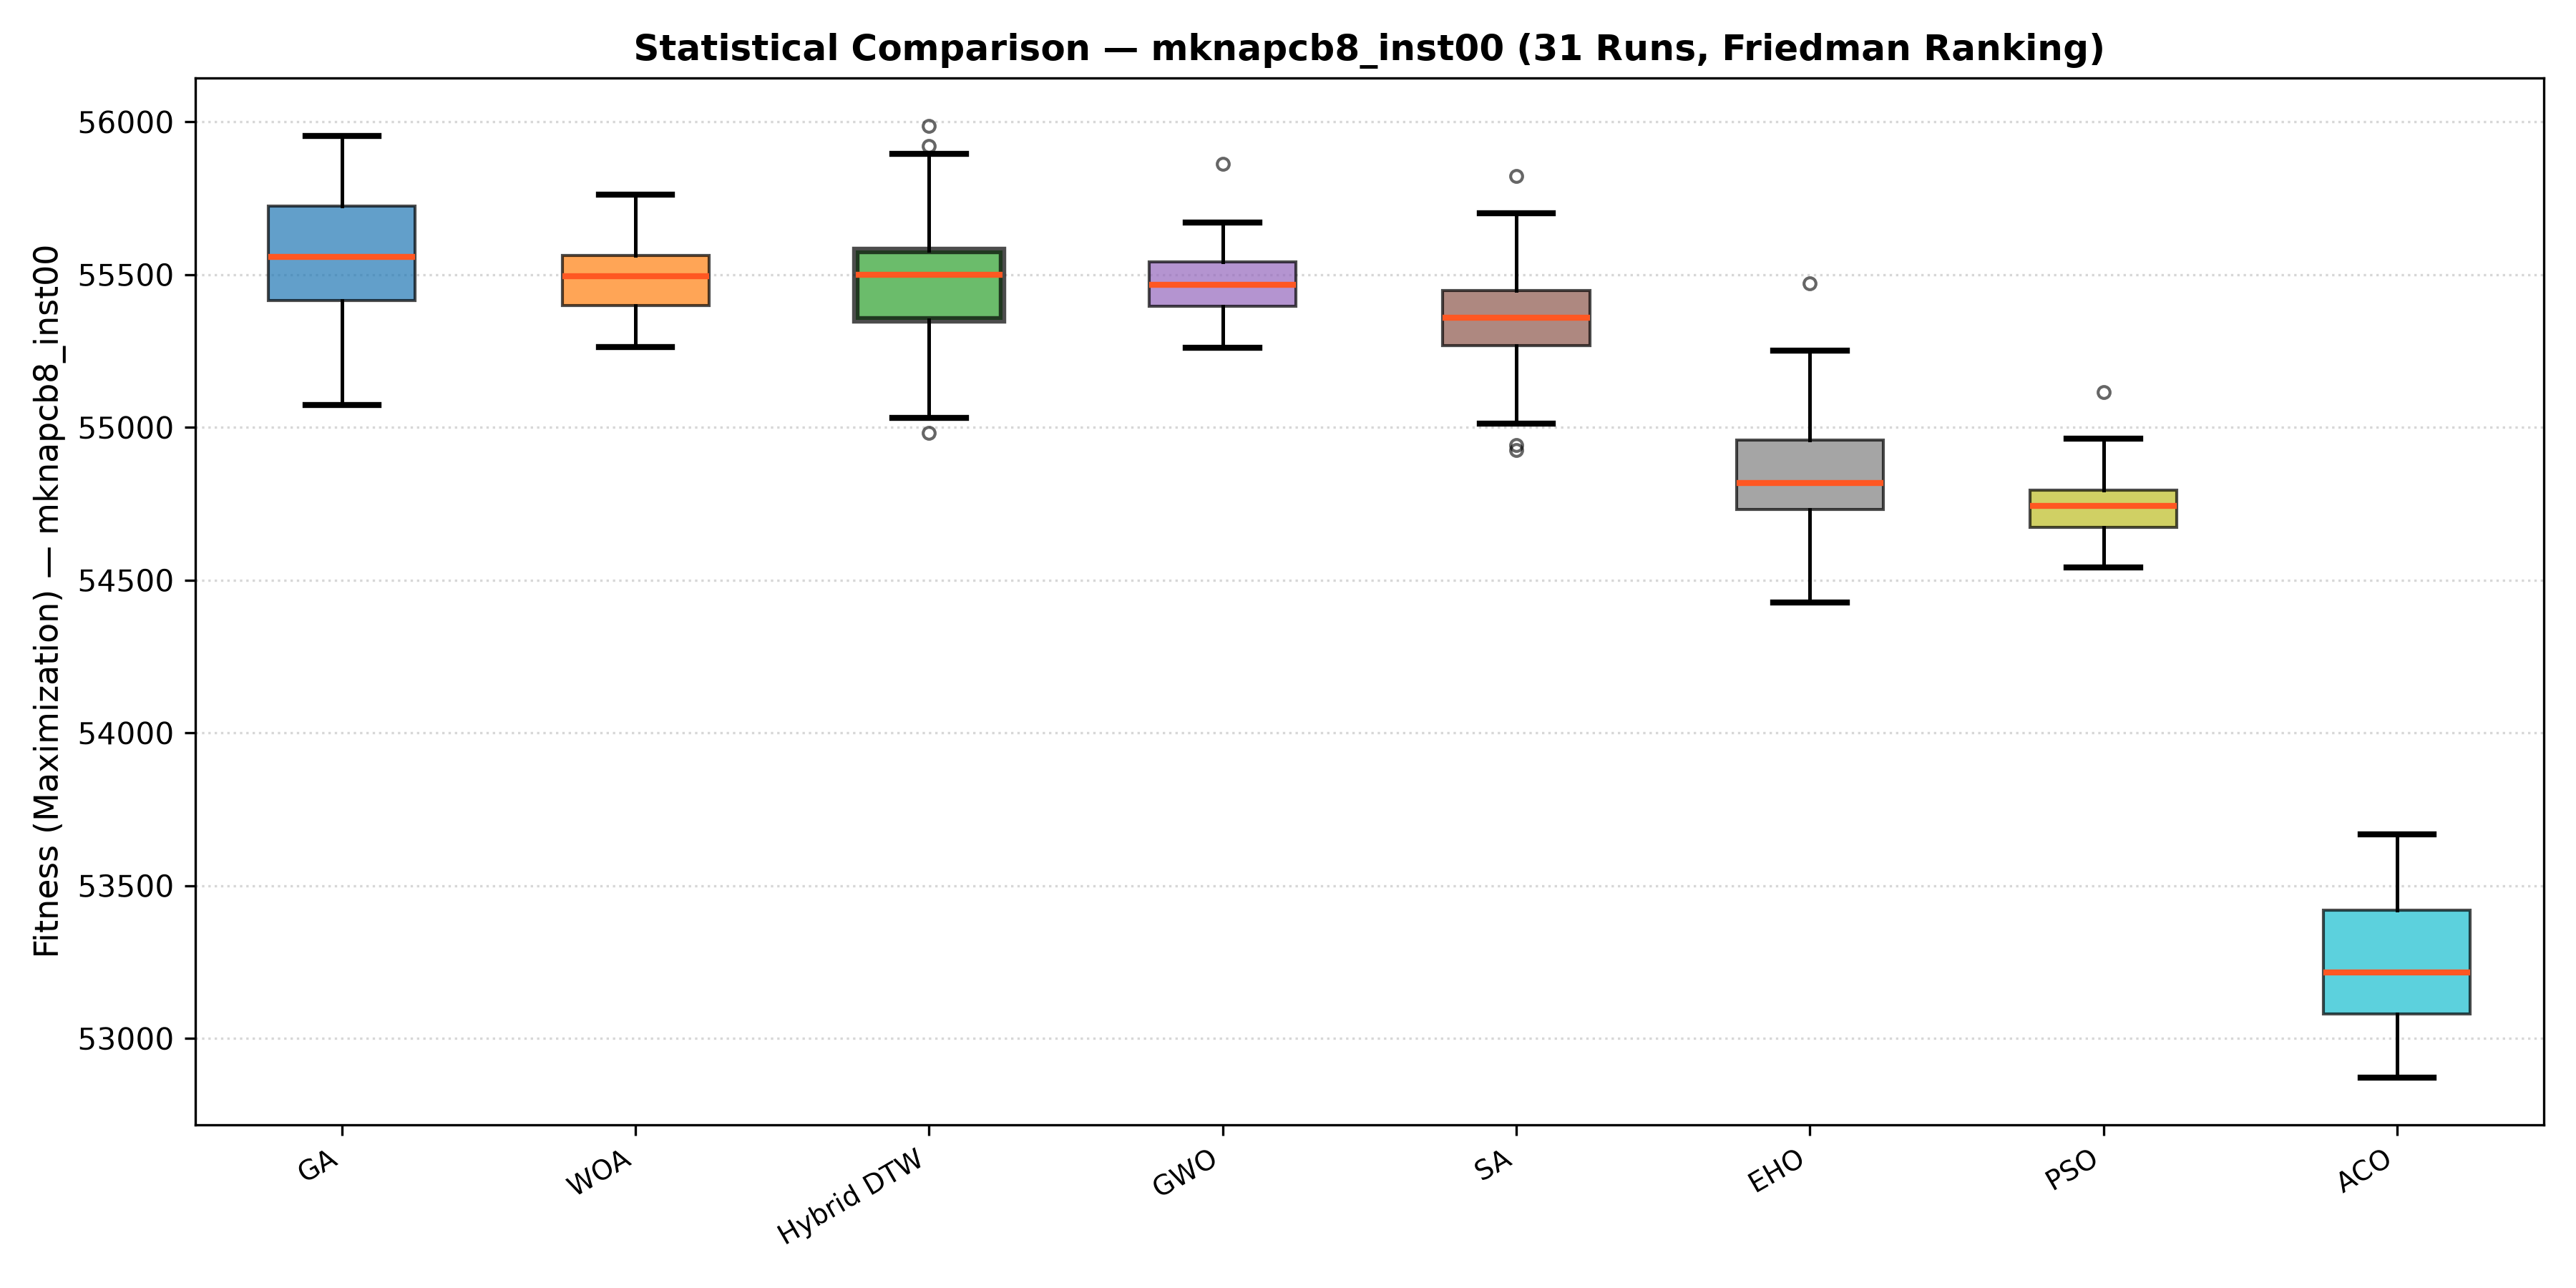
\includegraphics[width=0.32\textwidth]{imagenes_paper/mkp_dtw_3k_mknapcb8_comparativo_mh.png}}\hfill
\subfloat[Best-run convergence.]{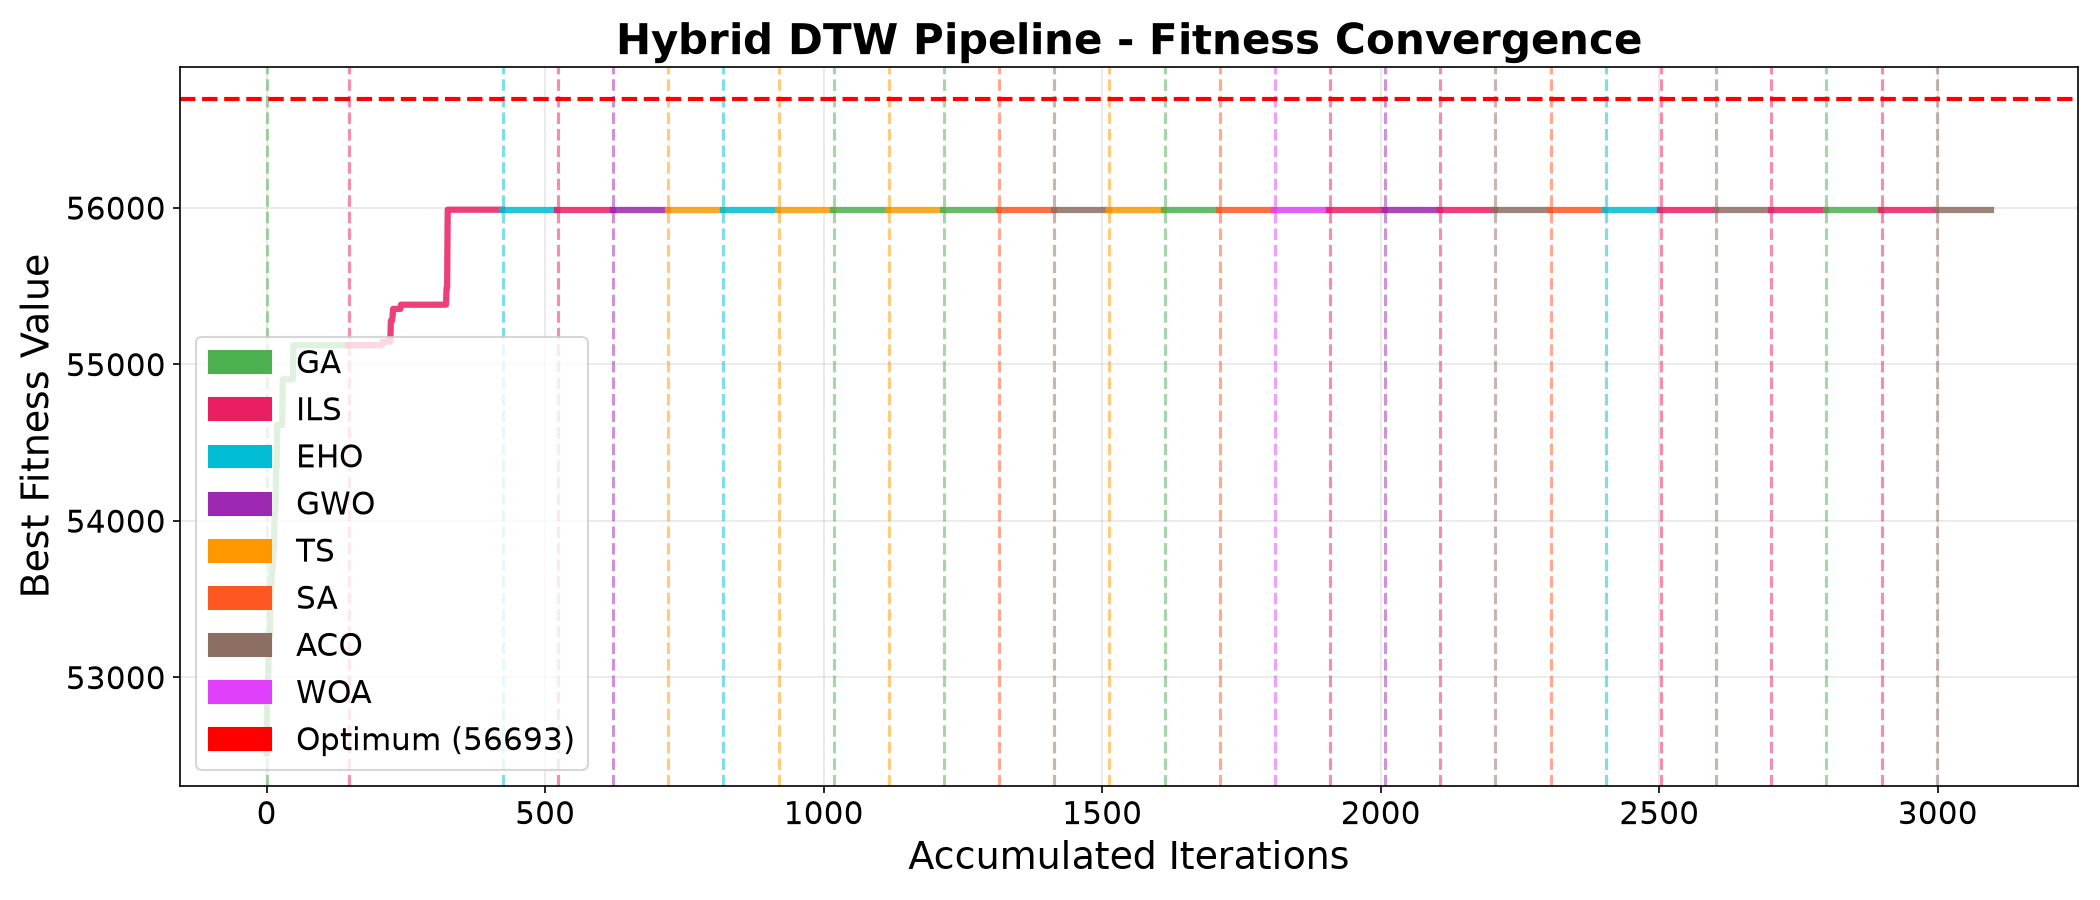
\includegraphics[width=0.32\textwidth]{imagenes_paper/mkp_dtw_3k_mknapcb8_convergencia.png}}\hfill
\subfloat[Elastic metric $\Delta=D_1-D_2$.]{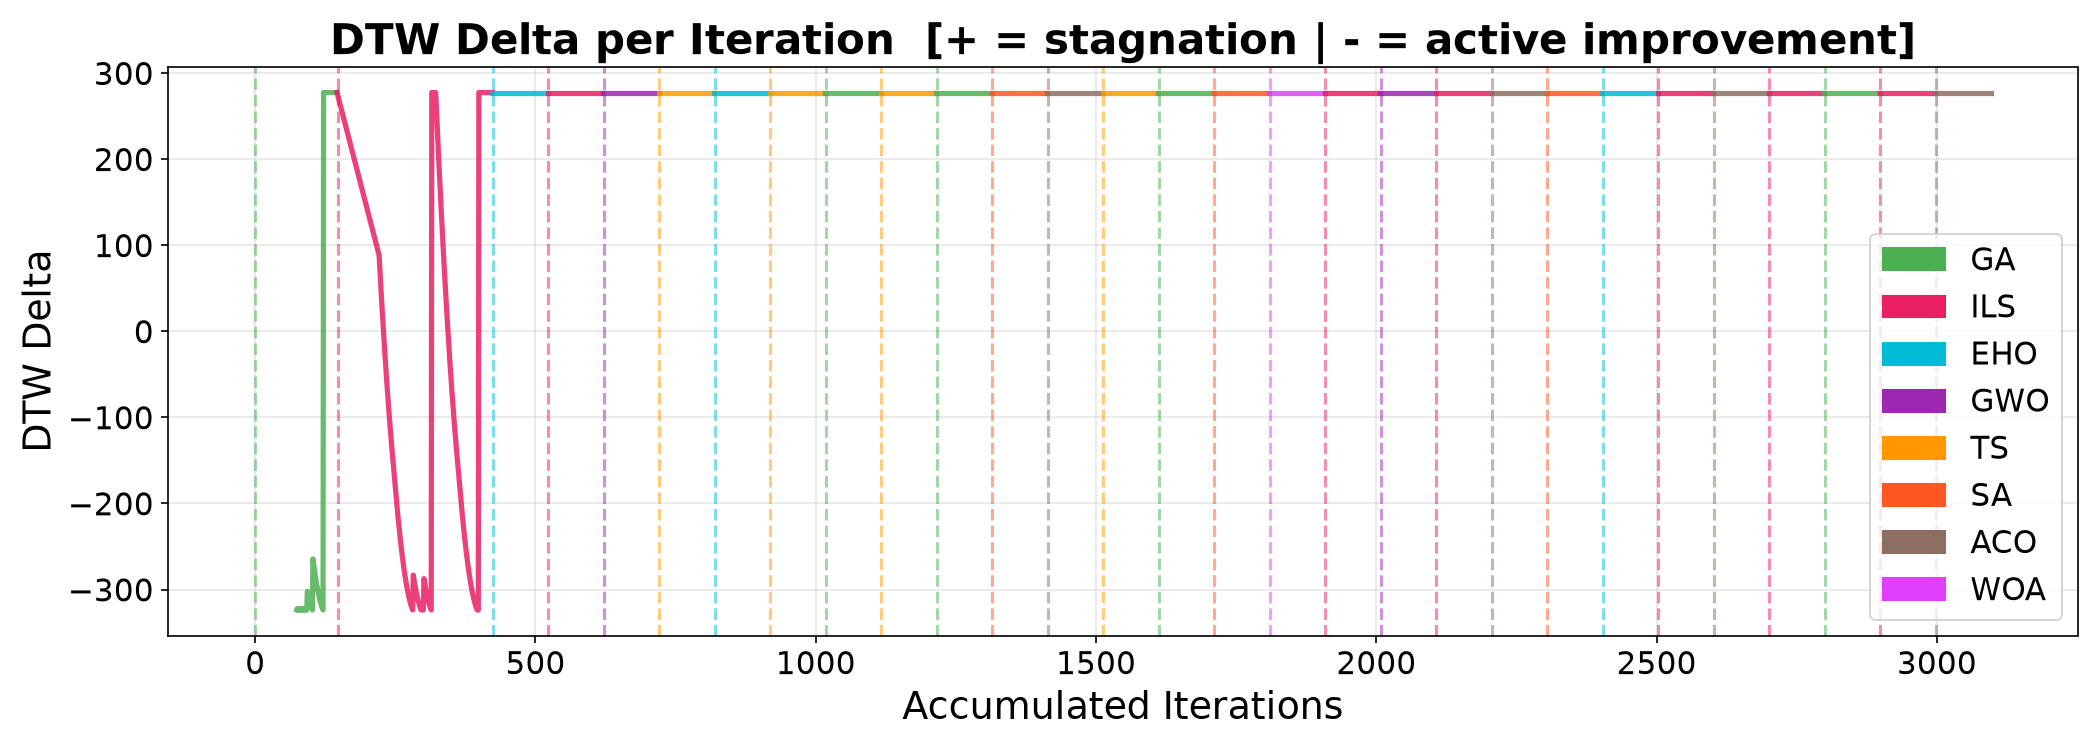
\includegraphics[width=0.32\textwidth]{imagenes_paper/mkp_dtw_3k_mknapcb8_delta.png}}
\caption{Diagnostic suite for instance \textbf{mknapcb8} ($n=250$, $m=30$) under the DTW framework with $T_{\max}=3{,}000$: (a)~final-fitness distribution over $N=31$ runs; (b)~convergence trajectory of the best run; (c)~elastic warping profile $\Delta$.}
\label{fig:mkp-best-cb8}
\end{figure}

% --- mknapcb9: DDTW, 3,000 iterations ---
\begin{figure}[htbp]
\centering
\subfloat[Metaheuristic comparison.]{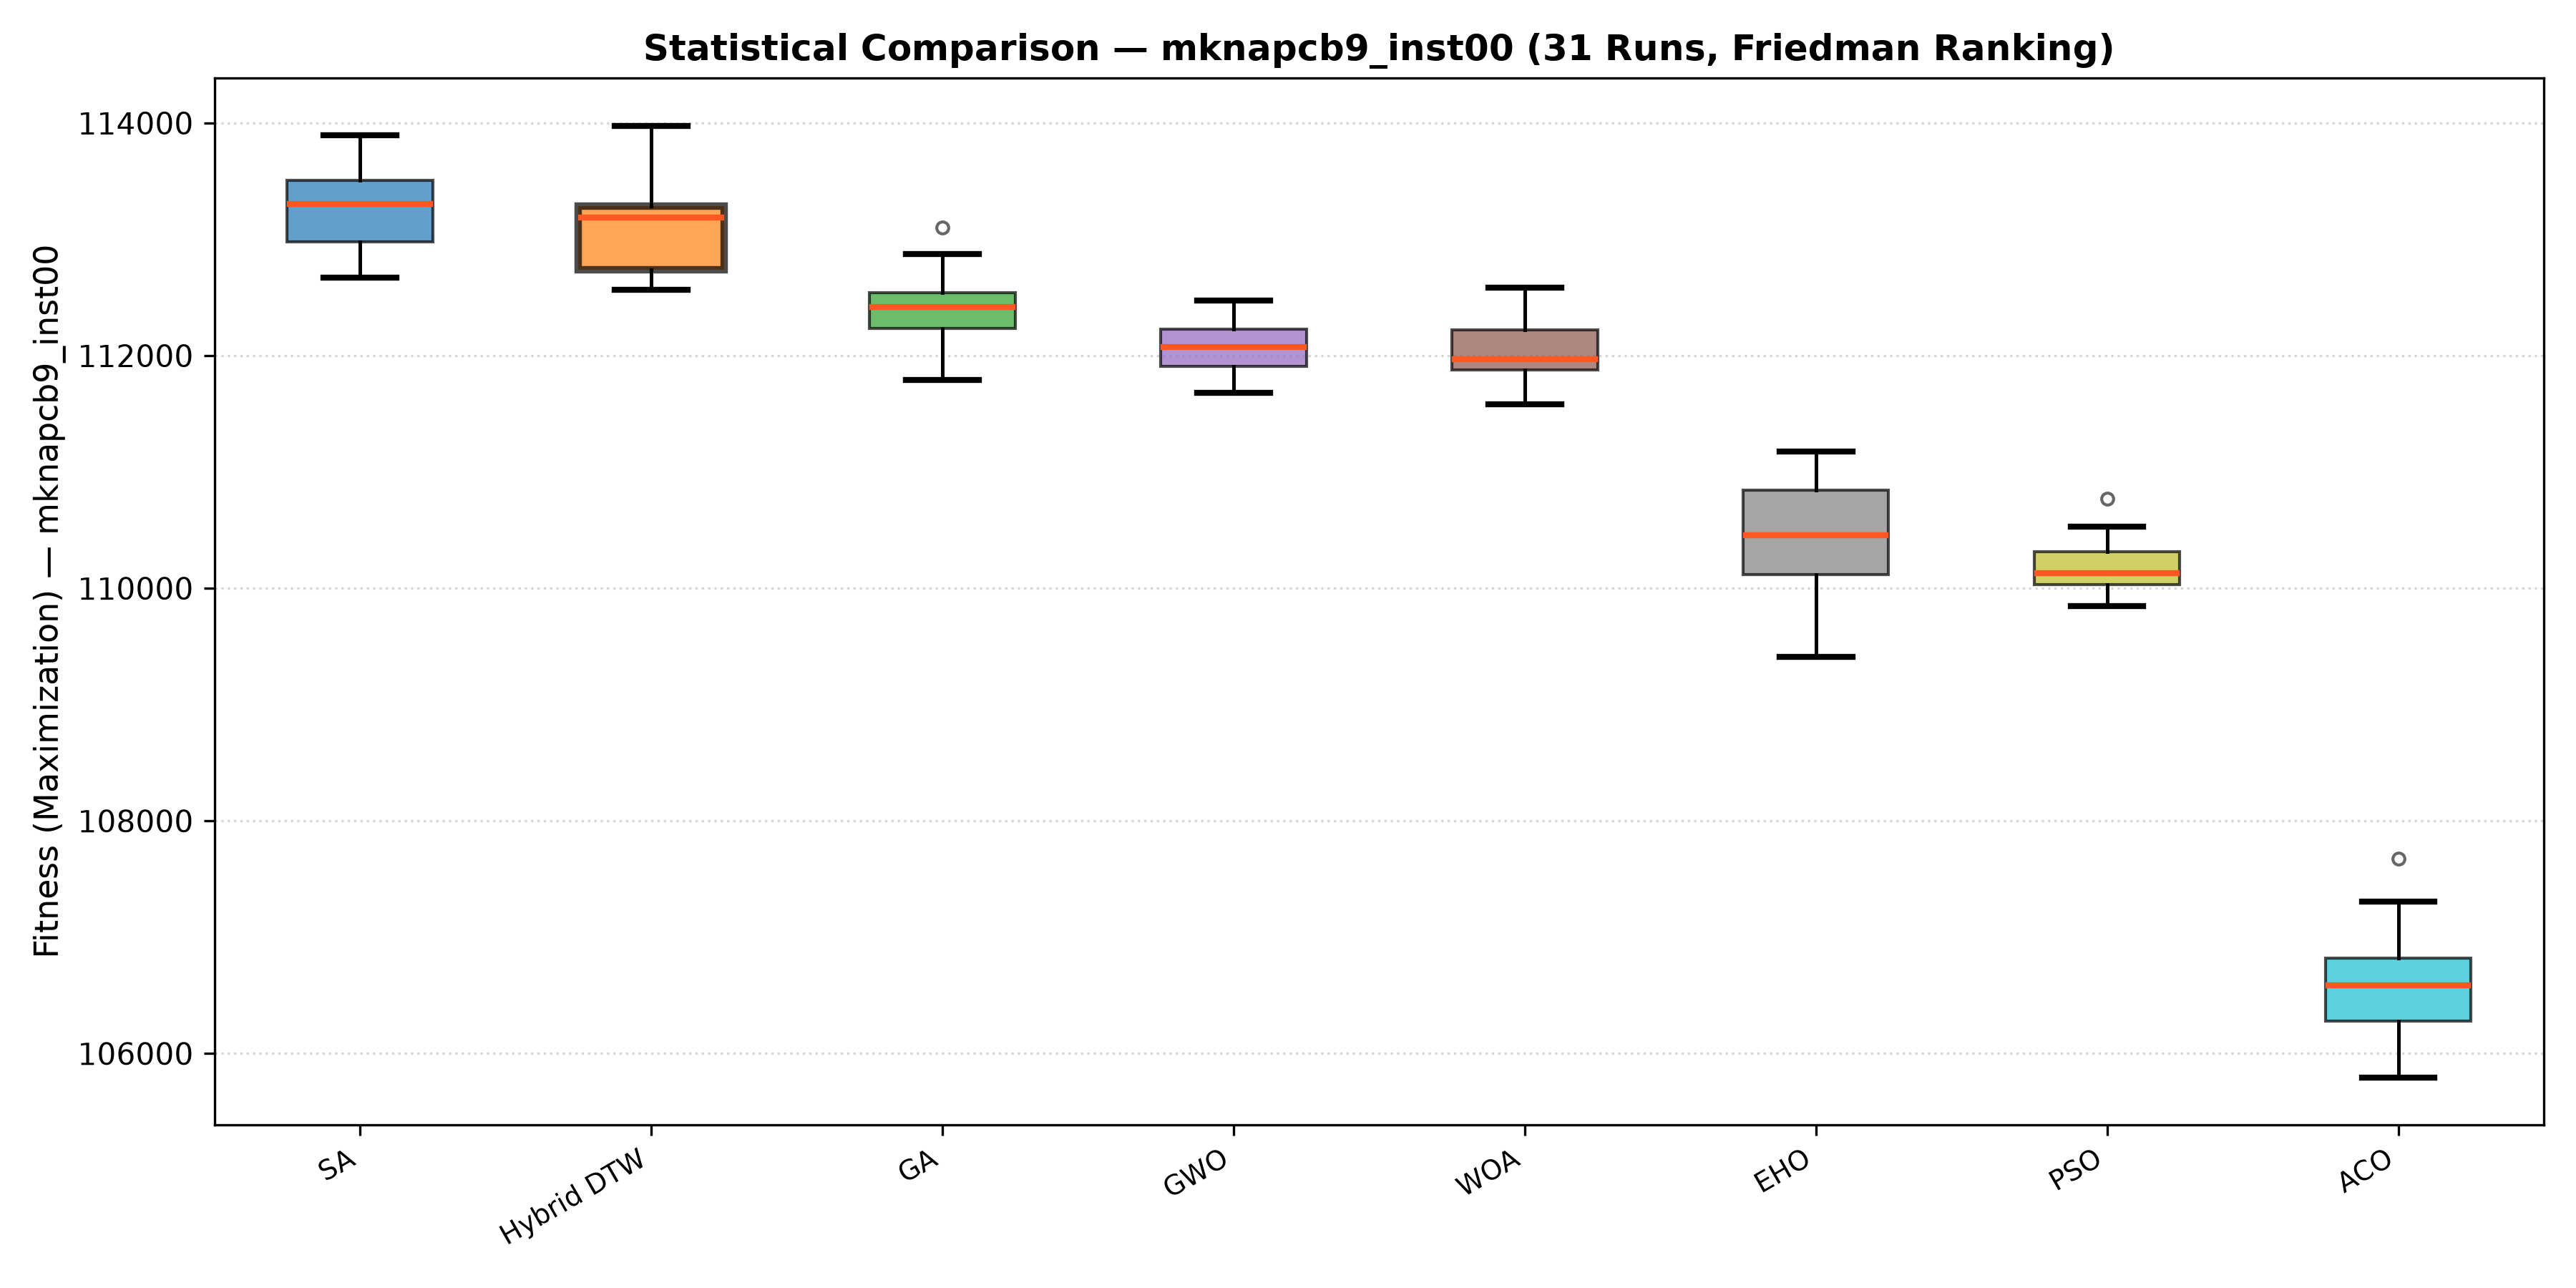
\includegraphics[width=0.32\textwidth]{imagenes_paper/mkp_ddtw_3k_mknapcb9_comparativo_mh.png}}\hfill
\subfloat[Best-run convergence.]{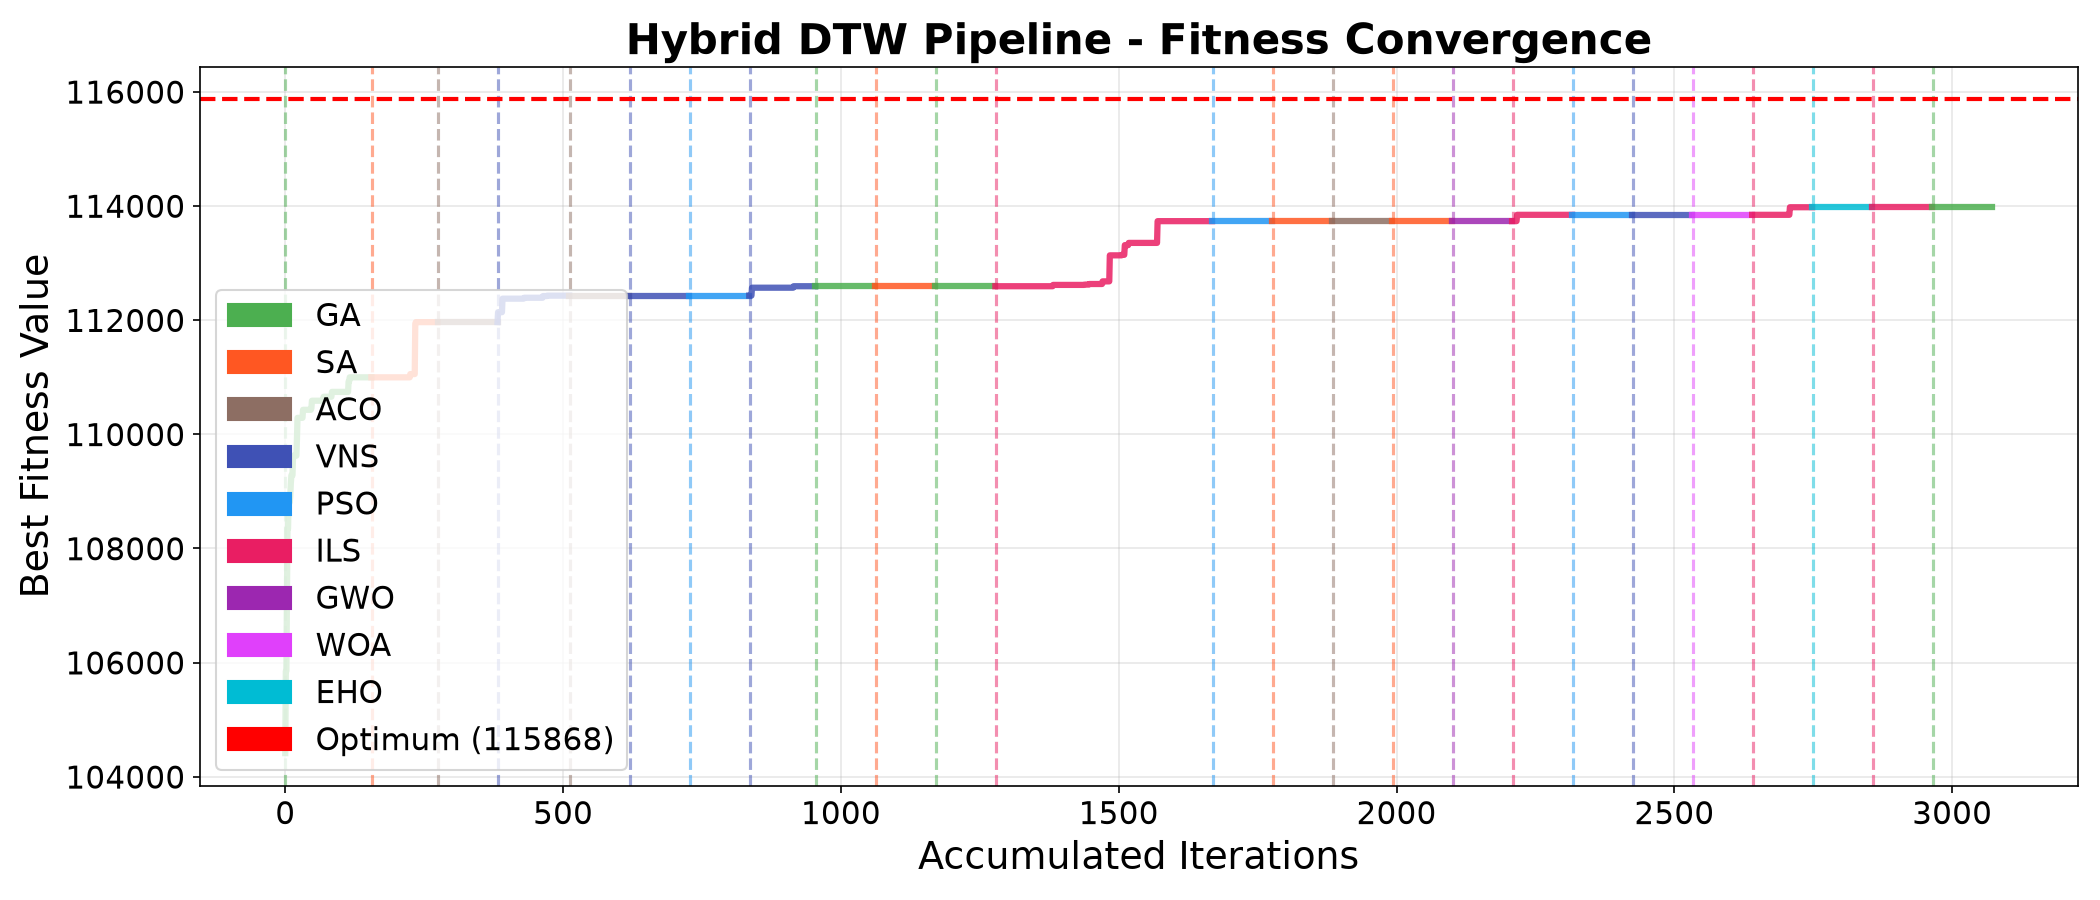
\includegraphics[width=0.32\textwidth]{imagenes_paper/mkp_ddtw_3k_mknapcb9_convergencia.png}}\hfill
\subfloat[Elastic metric $\Delta=D_1-D_2$.]{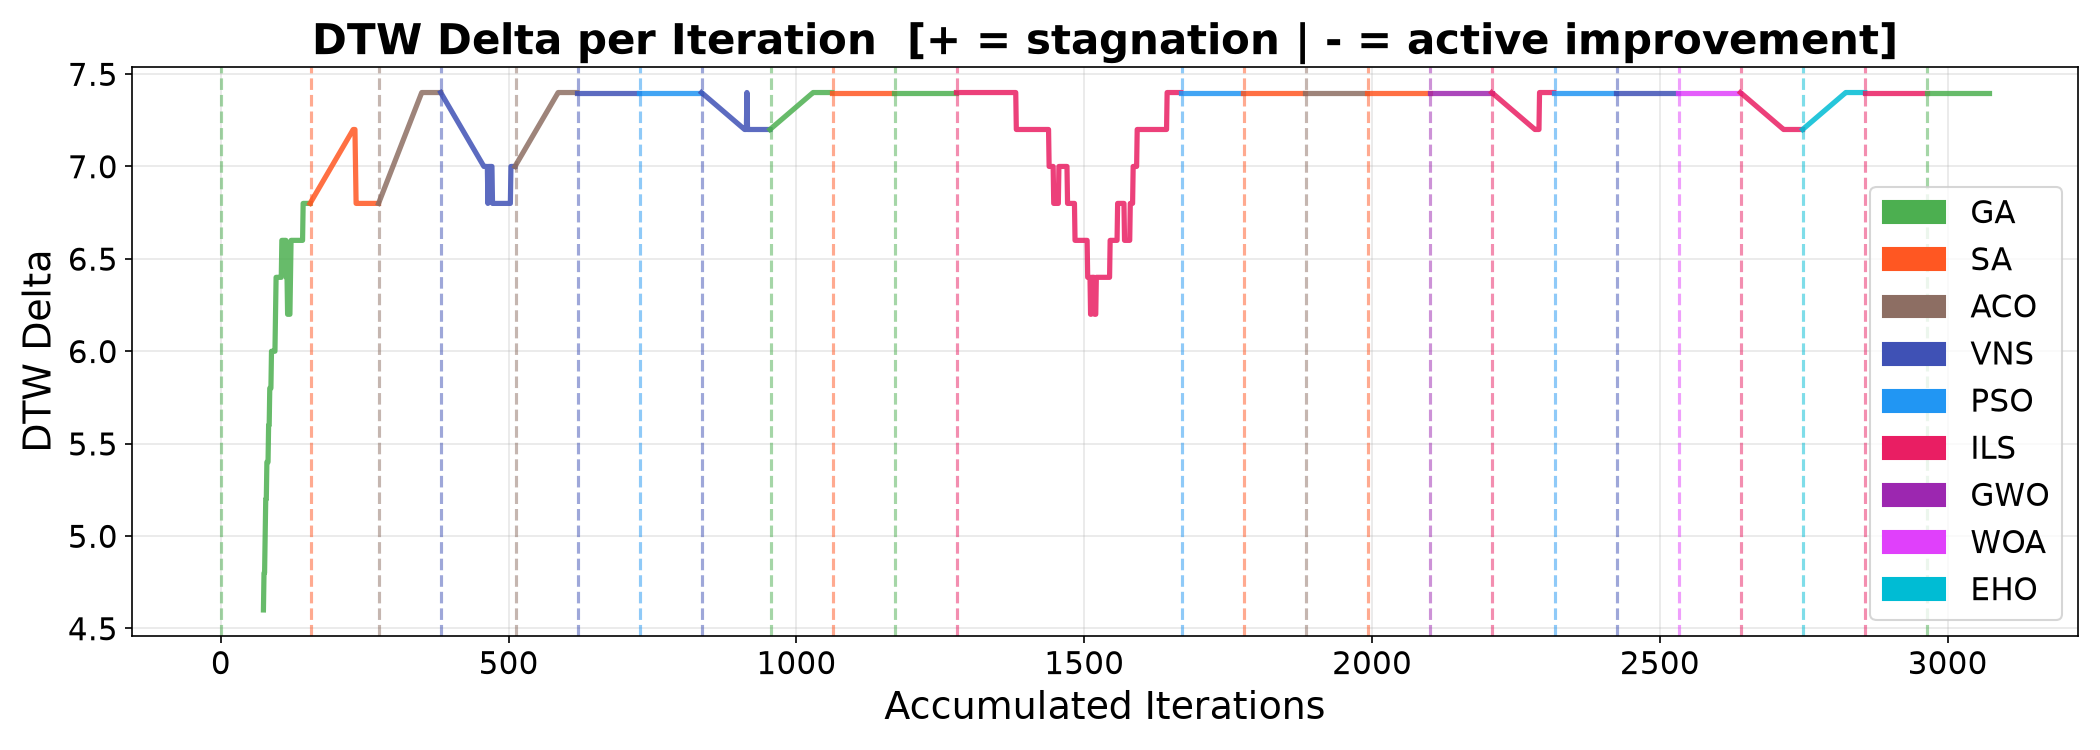
\includegraphics[width=0.32\textwidth]{imagenes_paper/mkp_ddtw_3k_mknapcb9_delta.png}}
\caption{Diagnostic suite for instance \textbf{mknapcb9} ($n=500$, $m=30$) under the DDTW framework with $T_{\max}=3{,}000$: (a)~final-fitness distribution over $N=31$ runs; (b)~convergence trajectory of the best run; (c)~elastic warping profile $\Delta$.}
\label{fig:mkp-best-cb9}
\end{figure}

% Required packages: graphicx, subfig (or subcaption with \subfloat redefined).

% Each figure shows the best-performing framework configuration for the
% corresponding instance, selected by highest mean fitness over 31 runs.
% DTW--3K is best for mknapcb1 and mknapcb3--mknapcb8;
% DDTW--3K is best for mknapcb2 and mknapcb9.

Figures~\ref{fig:mkp-best-cb1}--\ref{fig:mkp-best-cb9} present the
diagnostic suite for each of the nine Chu--Beasley MKP instances under its
best-performing framework configuration, selected by highest mean fitness
over the 31 runs, with corresponding executions treated as paired. DTW with $T_{\max}=3{,}000$ achieved the
highest mean in seven instances (mknapcb1 and mknapcb3--mknapcb8), while
DDTW with $T_{\max}=3{,}000$ was superior for mknapcb2 and mknapcb9.
Each figure comprises three panels: (a)~a box-plot comparing the
final-fitness distributions of the hybrid framework against the standalone
metaheuristics over the 31 runs, allowing visual assessment of both central
tendency and dispersion; (b)~the convergence trajectory of the best run,
showing the evolution of the incumbent fitness along with the solver
transitions triggered by the stagnation monitor; and (c)~the elastic
warping profile $\Delta = D_1 - D_2$, where positive values indicate
detected stagnation phases and negative values correspond to periods of
active improvement.

% --- mknapcb1: DTW, 3,000 iterations ---
\begin{figure}[htbp]
\centering
\subfloat[Metaheuristic comparison.]{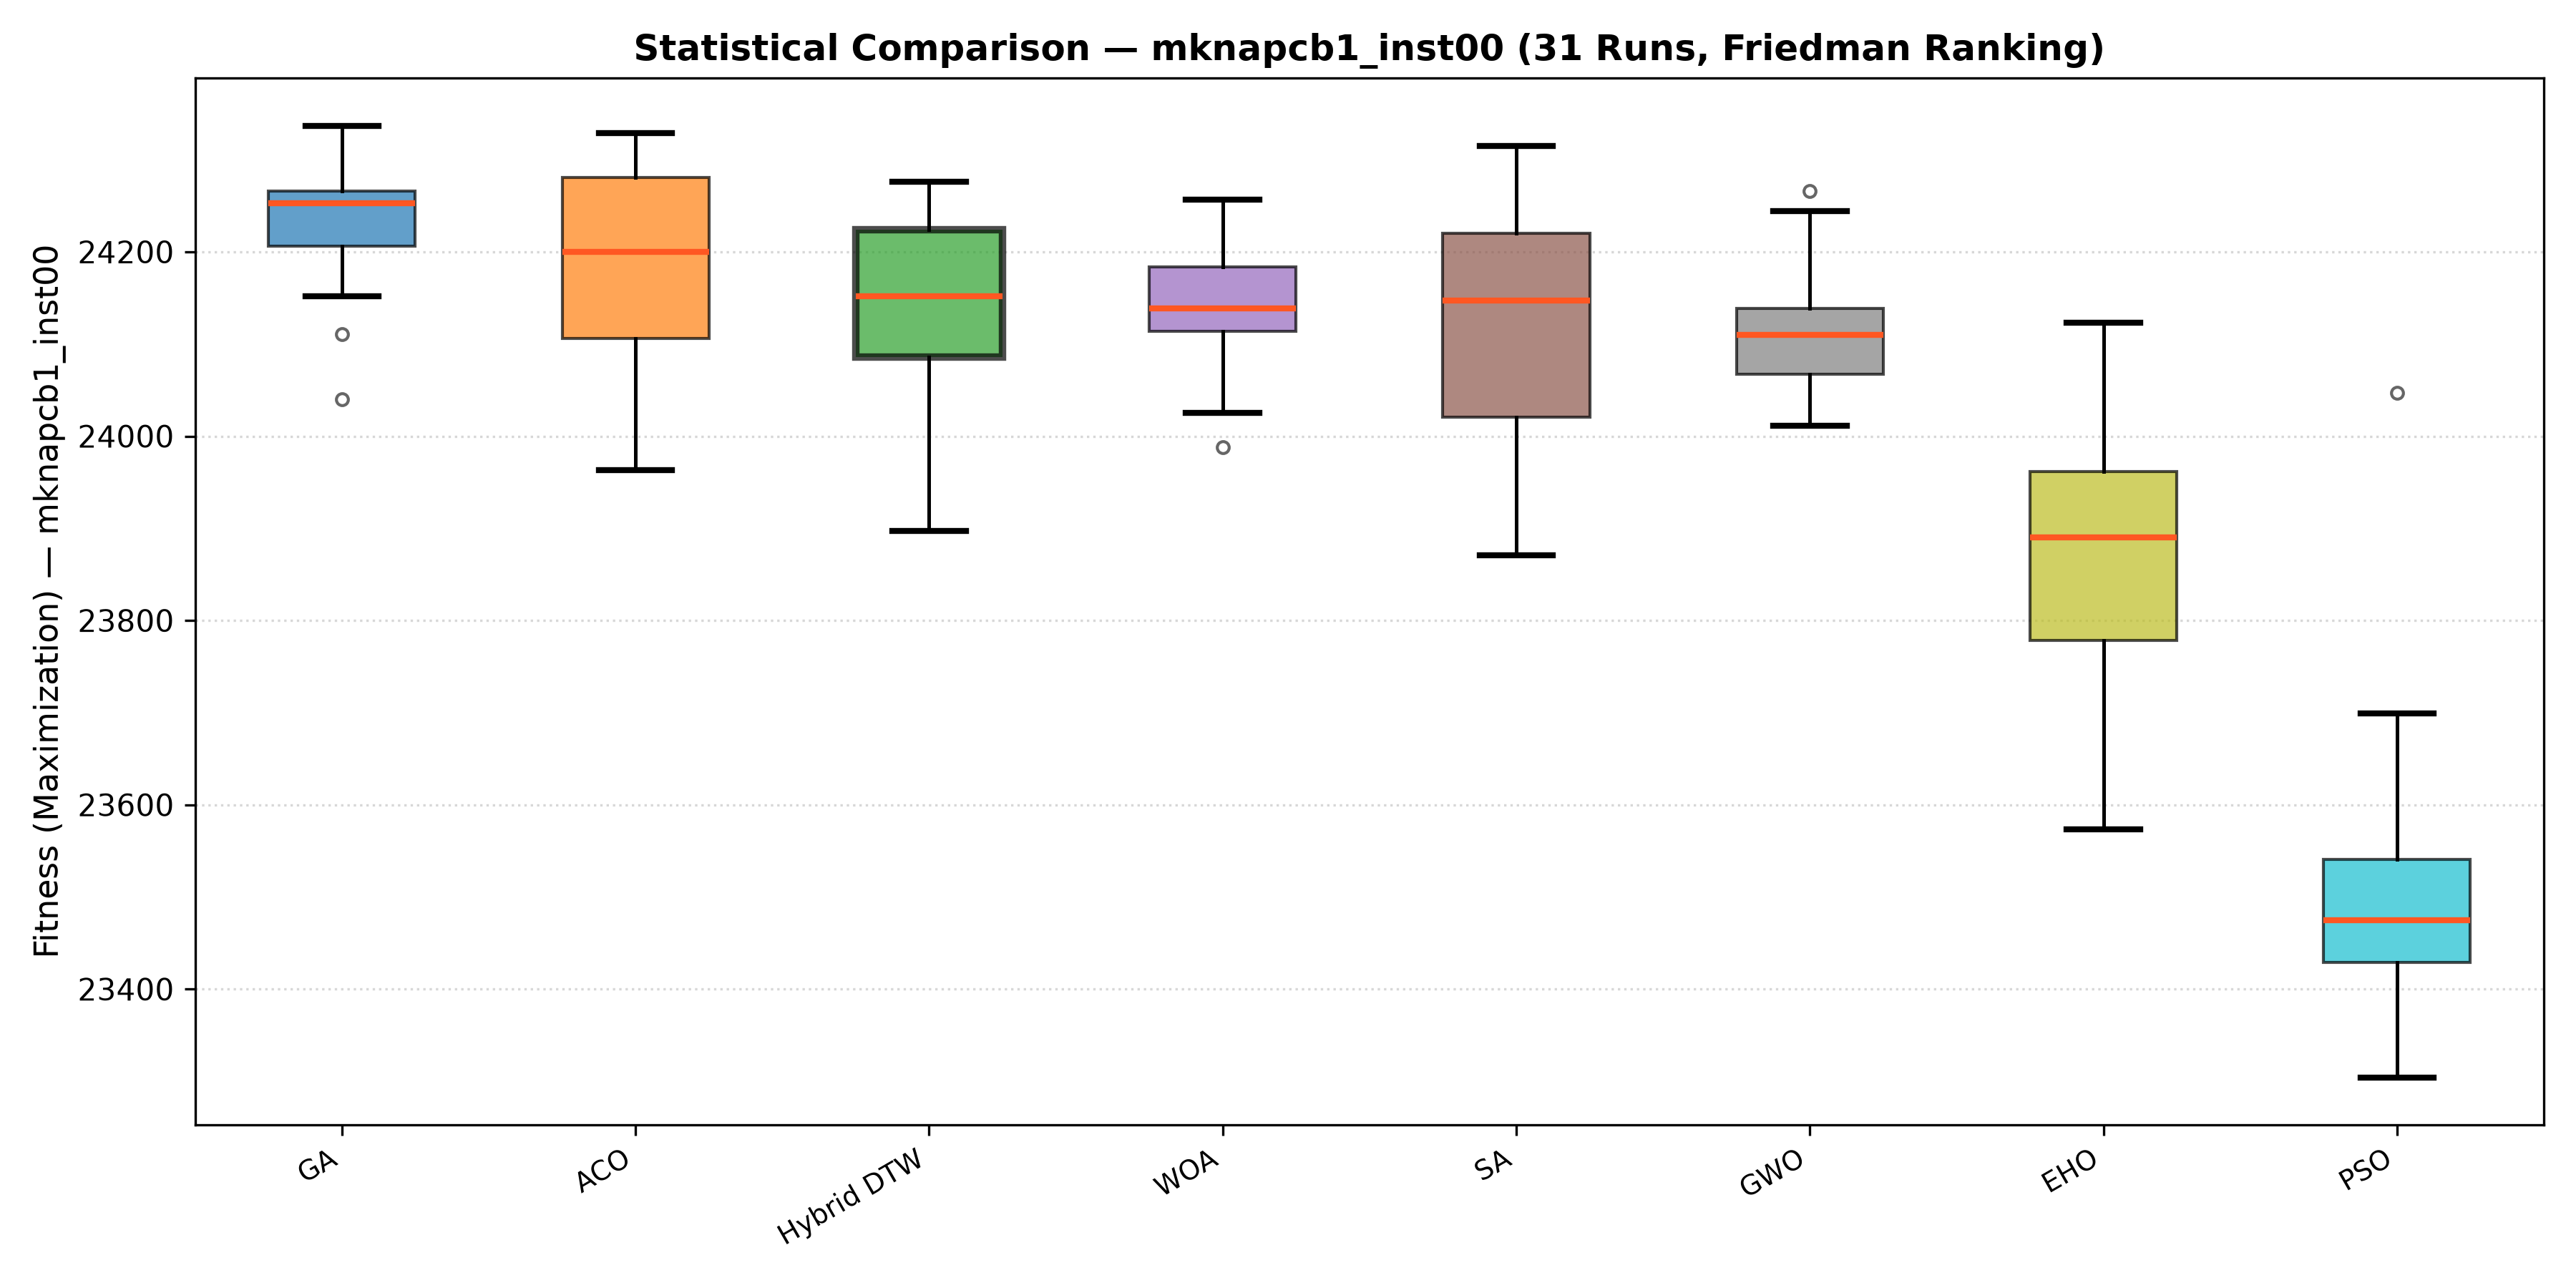
\includegraphics[width=0.32\textwidth]{imagenes_paper/mkp_dtw_3k_mknapcb1_comparativo_mh.png}}\hfill
\subfloat[Best-run convergence.]{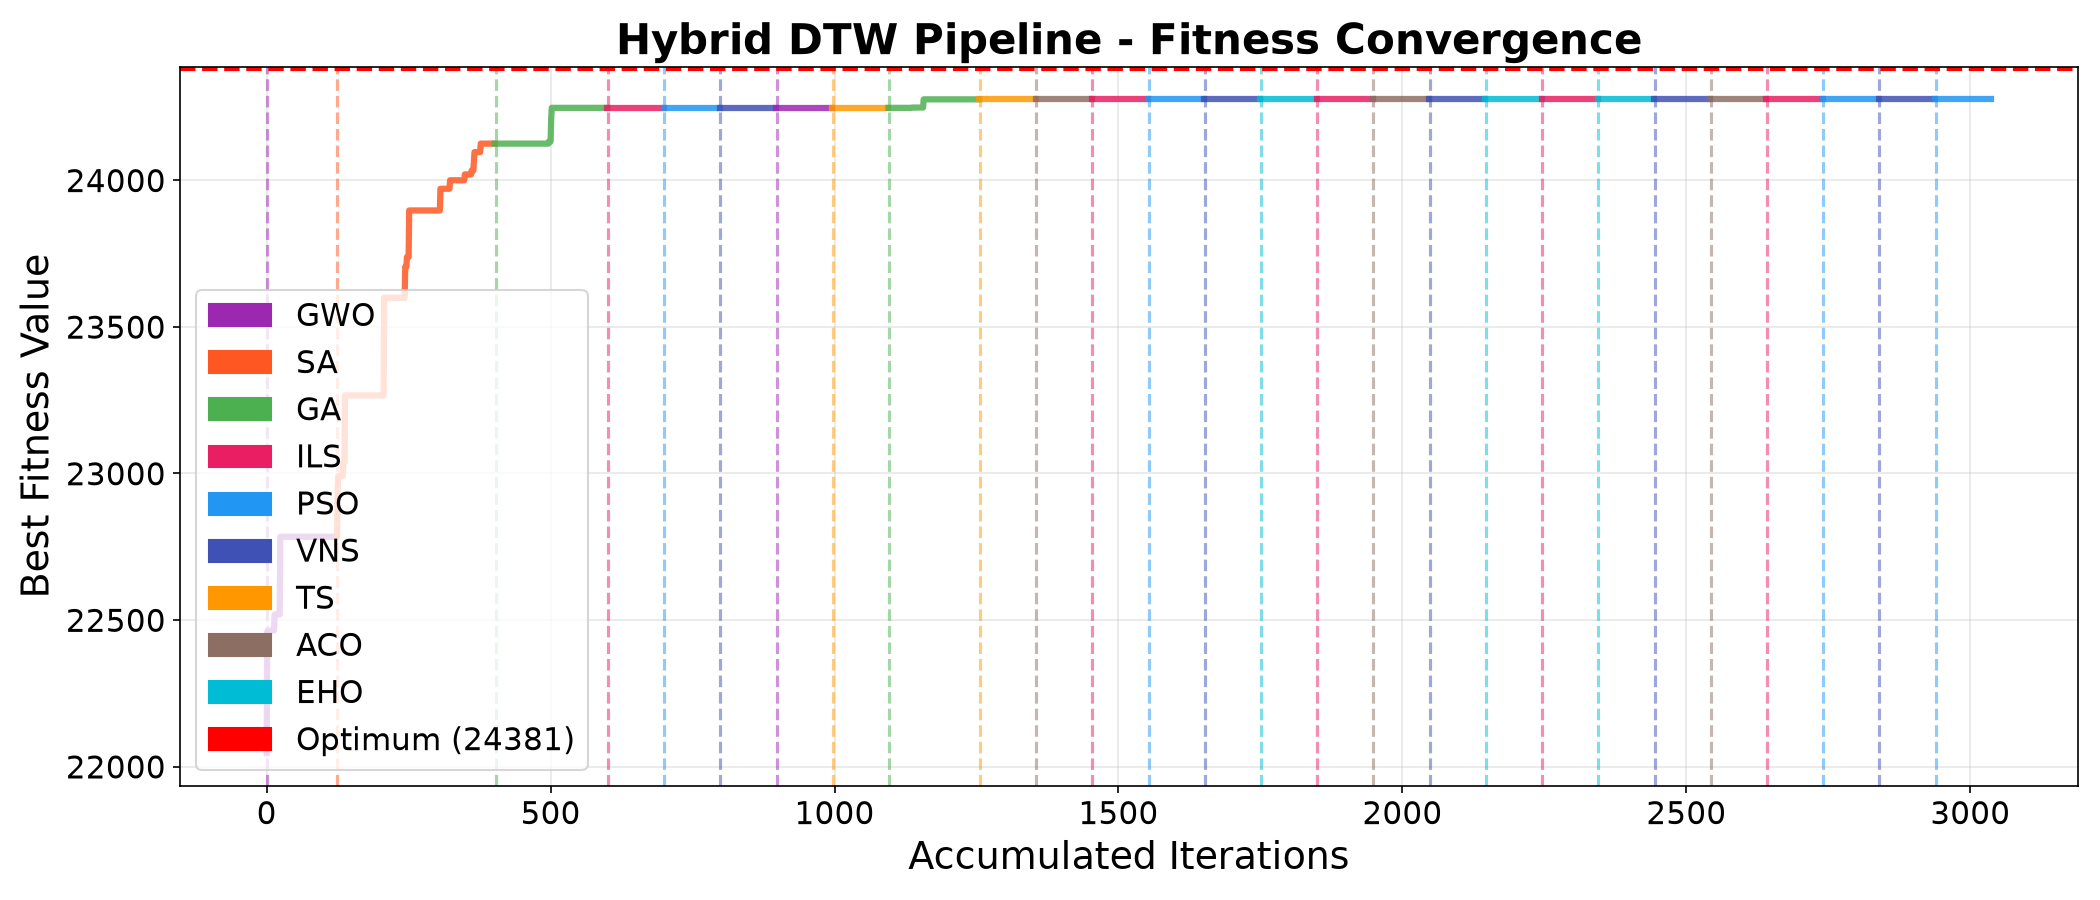
\includegraphics[width=0.32\textwidth]{imagenes_paper/mkp_dtw_3k_mknapcb1_convergencia.png}}\hfill
\subfloat[Elastic metric $\Delta=D_1-D_2$.]{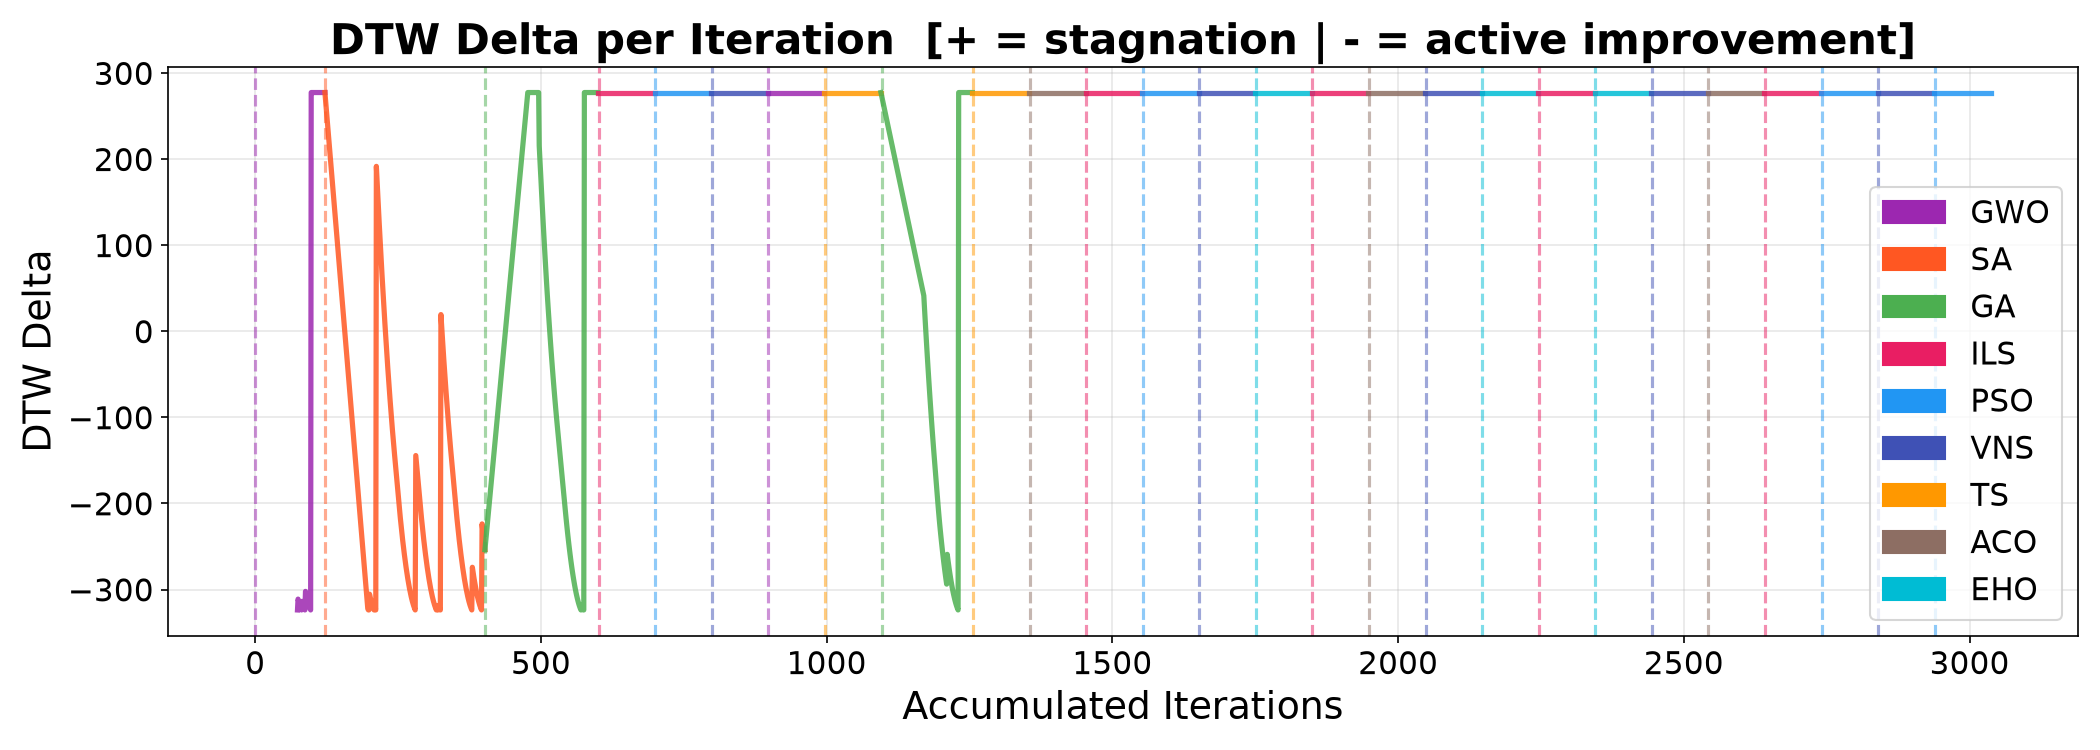
\includegraphics[width=0.32\textwidth]{imagenes_paper/mkp_dtw_3k_mknapcb1_delta.png}}
\caption{Diagnostic suite for instance \textbf{mknapcb1} ($n=100$, $m=5$) under the DTW framework with $T_{\max}=3{,}000$: (a)~final-fitness distribution over $N=31$ runs; (b)~convergence trajectory of the best run; (c)~elastic warping profile $\Delta$.}
\label{fig:mkp-best-cb1}
\end{figure}

% --- mknapcb2: DDTW, 3,000 iterations ---
\begin{figure}[htbp]
\centering
\subfloat[Metaheuristic comparison.]{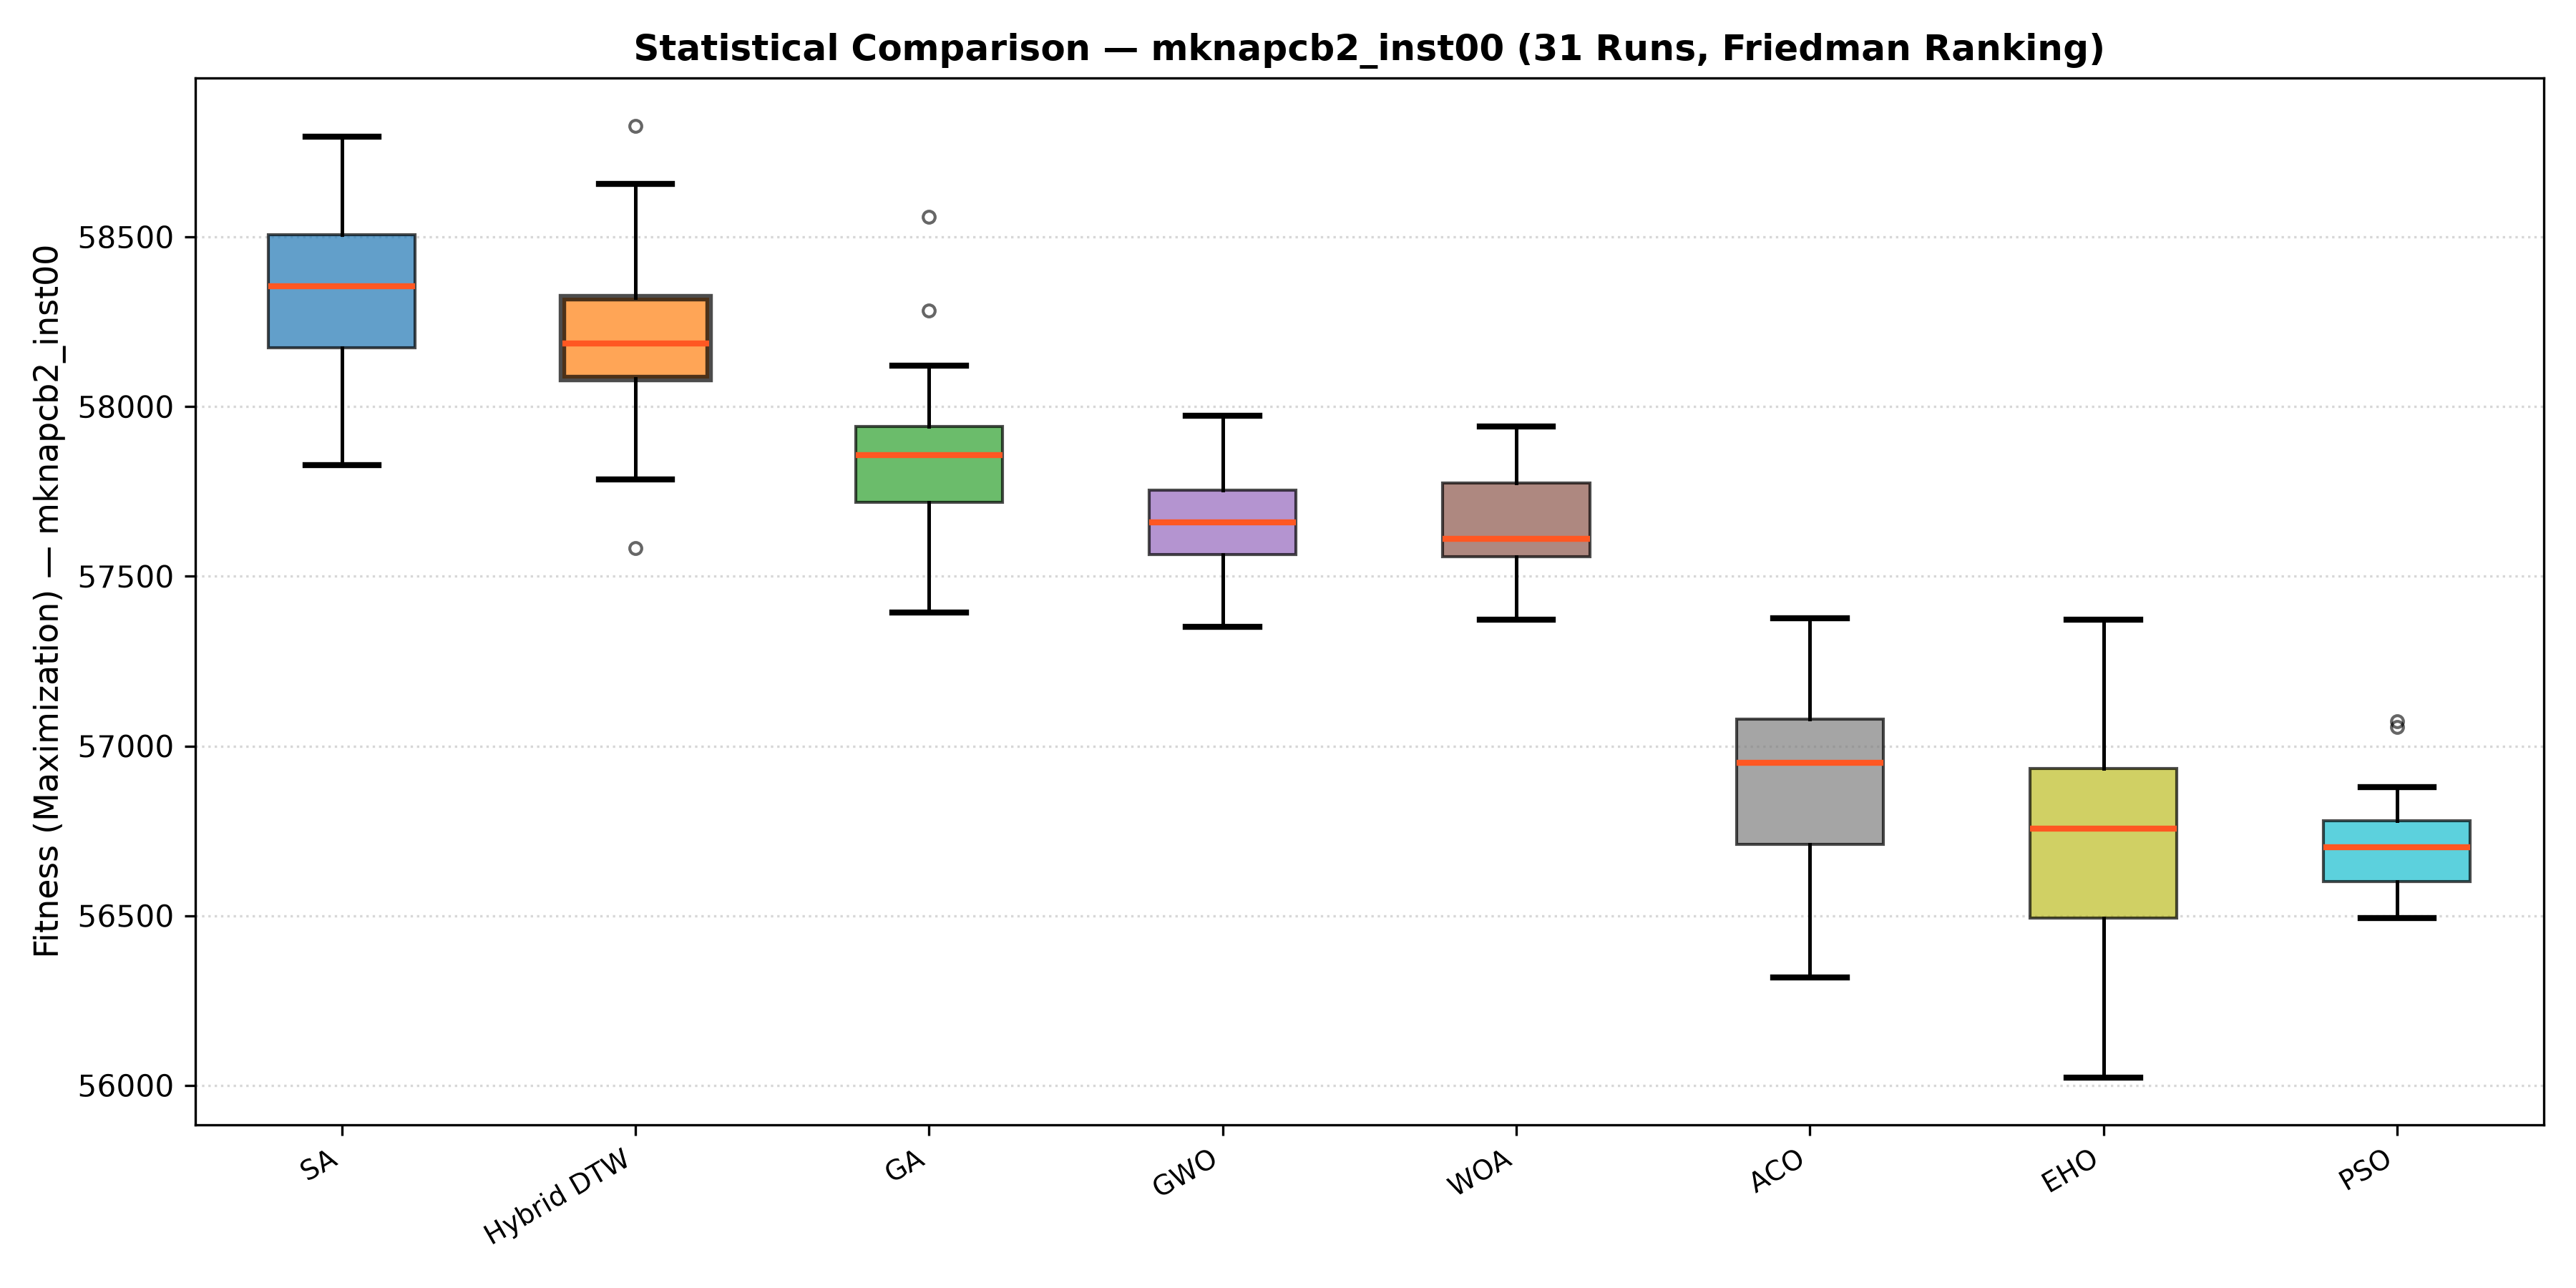
\includegraphics[width=0.32\textwidth]{imagenes_paper/mkp_ddtw_3k_mknapcb2_comparativo_mh.png}}\hfill
\subfloat[Best-run convergence.]{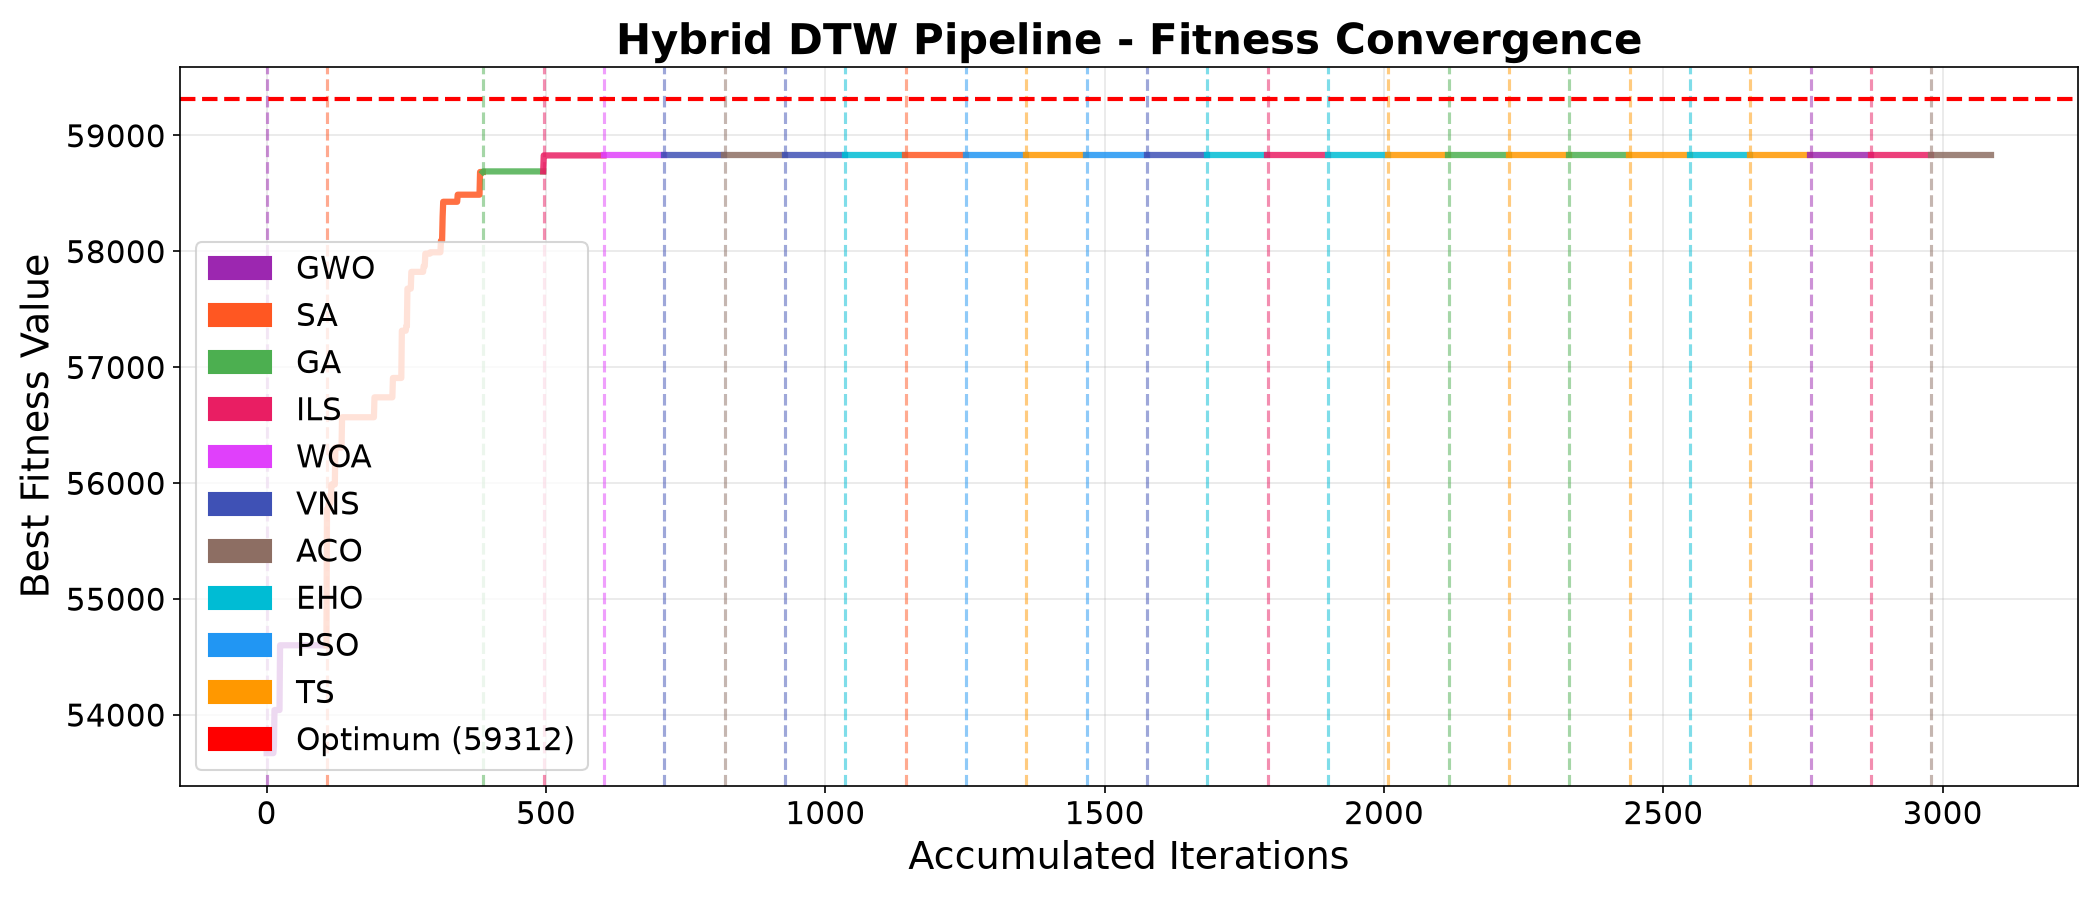
\includegraphics[width=0.32\textwidth]{imagenes_paper/mkp_ddtw_3k_mknapcb2_convergencia.png}}\hfill
\subfloat[Elastic metric $\Delta=D_1-D_2$.]{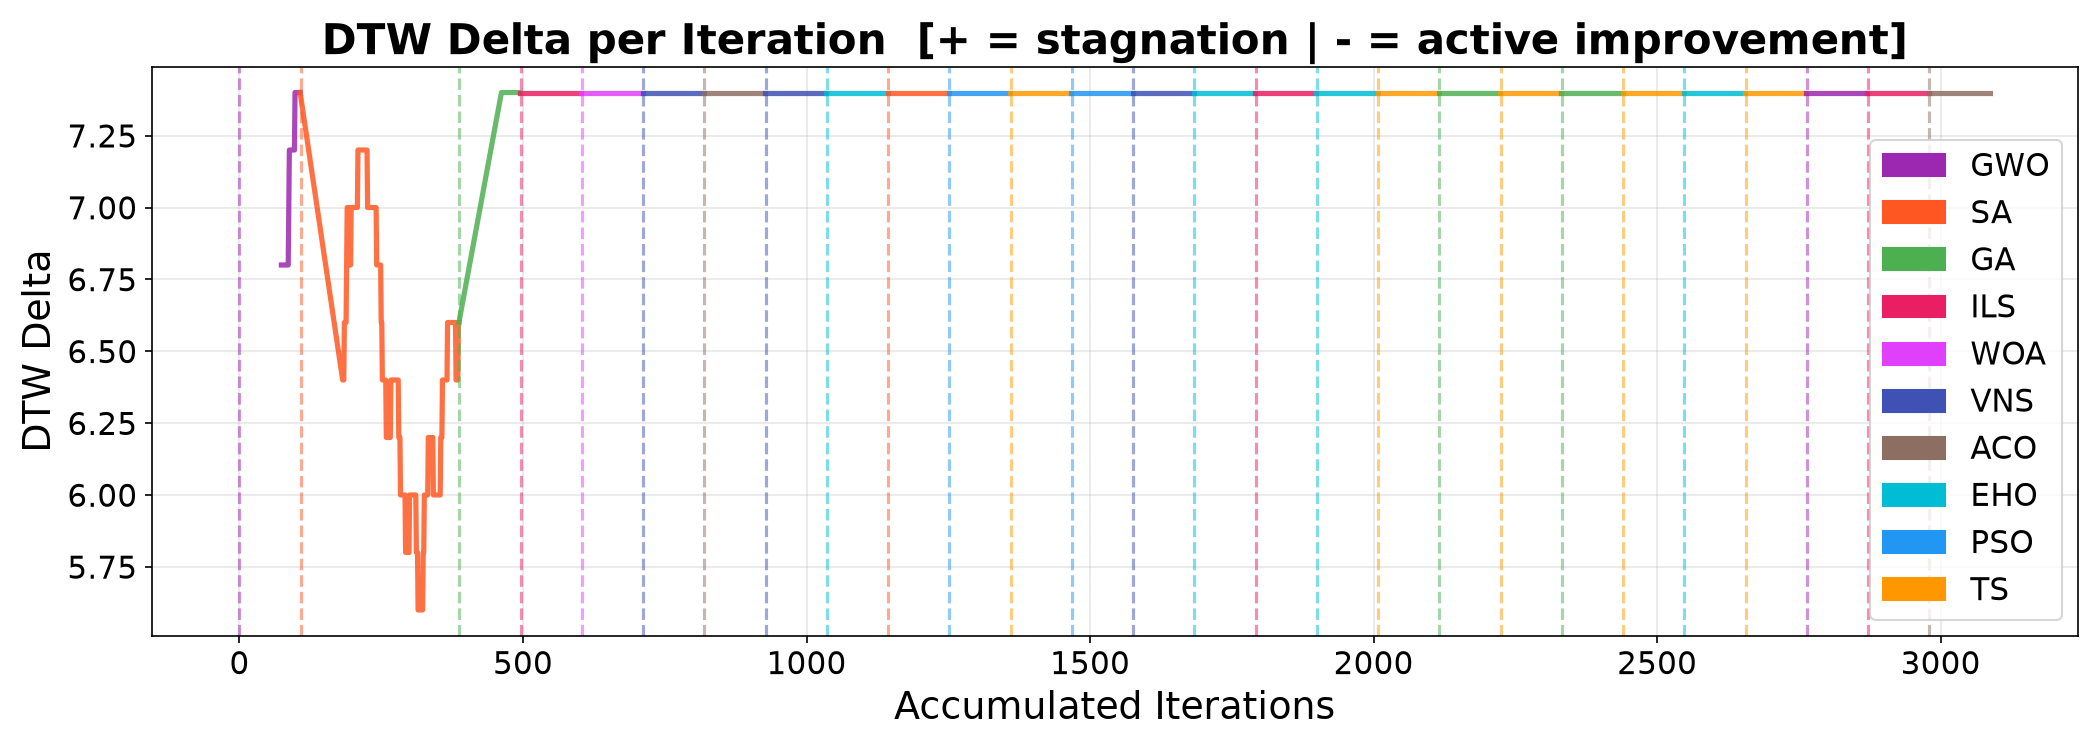
\includegraphics[width=0.32\textwidth]{imagenes_paper/mkp_ddtw_3k_mknapcb2_delta.png}}
\caption{Diagnostic suite for instance \textbf{mknapcb2} ($n=250$, $m=5$) under the DDTW framework with $T_{\max}=3{,}000$: (a)~final-fitness distribution over $N=31$ runs; (b)~convergence trajectory of the best run; (c)~elastic warping profile $\Delta$.}
\label{fig:mkp-best-cb2}
\end{figure}

% --- mknapcb3: DTW, 3,000 iterations ---
\begin{figure}[htbp]
\centering
\subfloat[Metaheuristic comparison.]{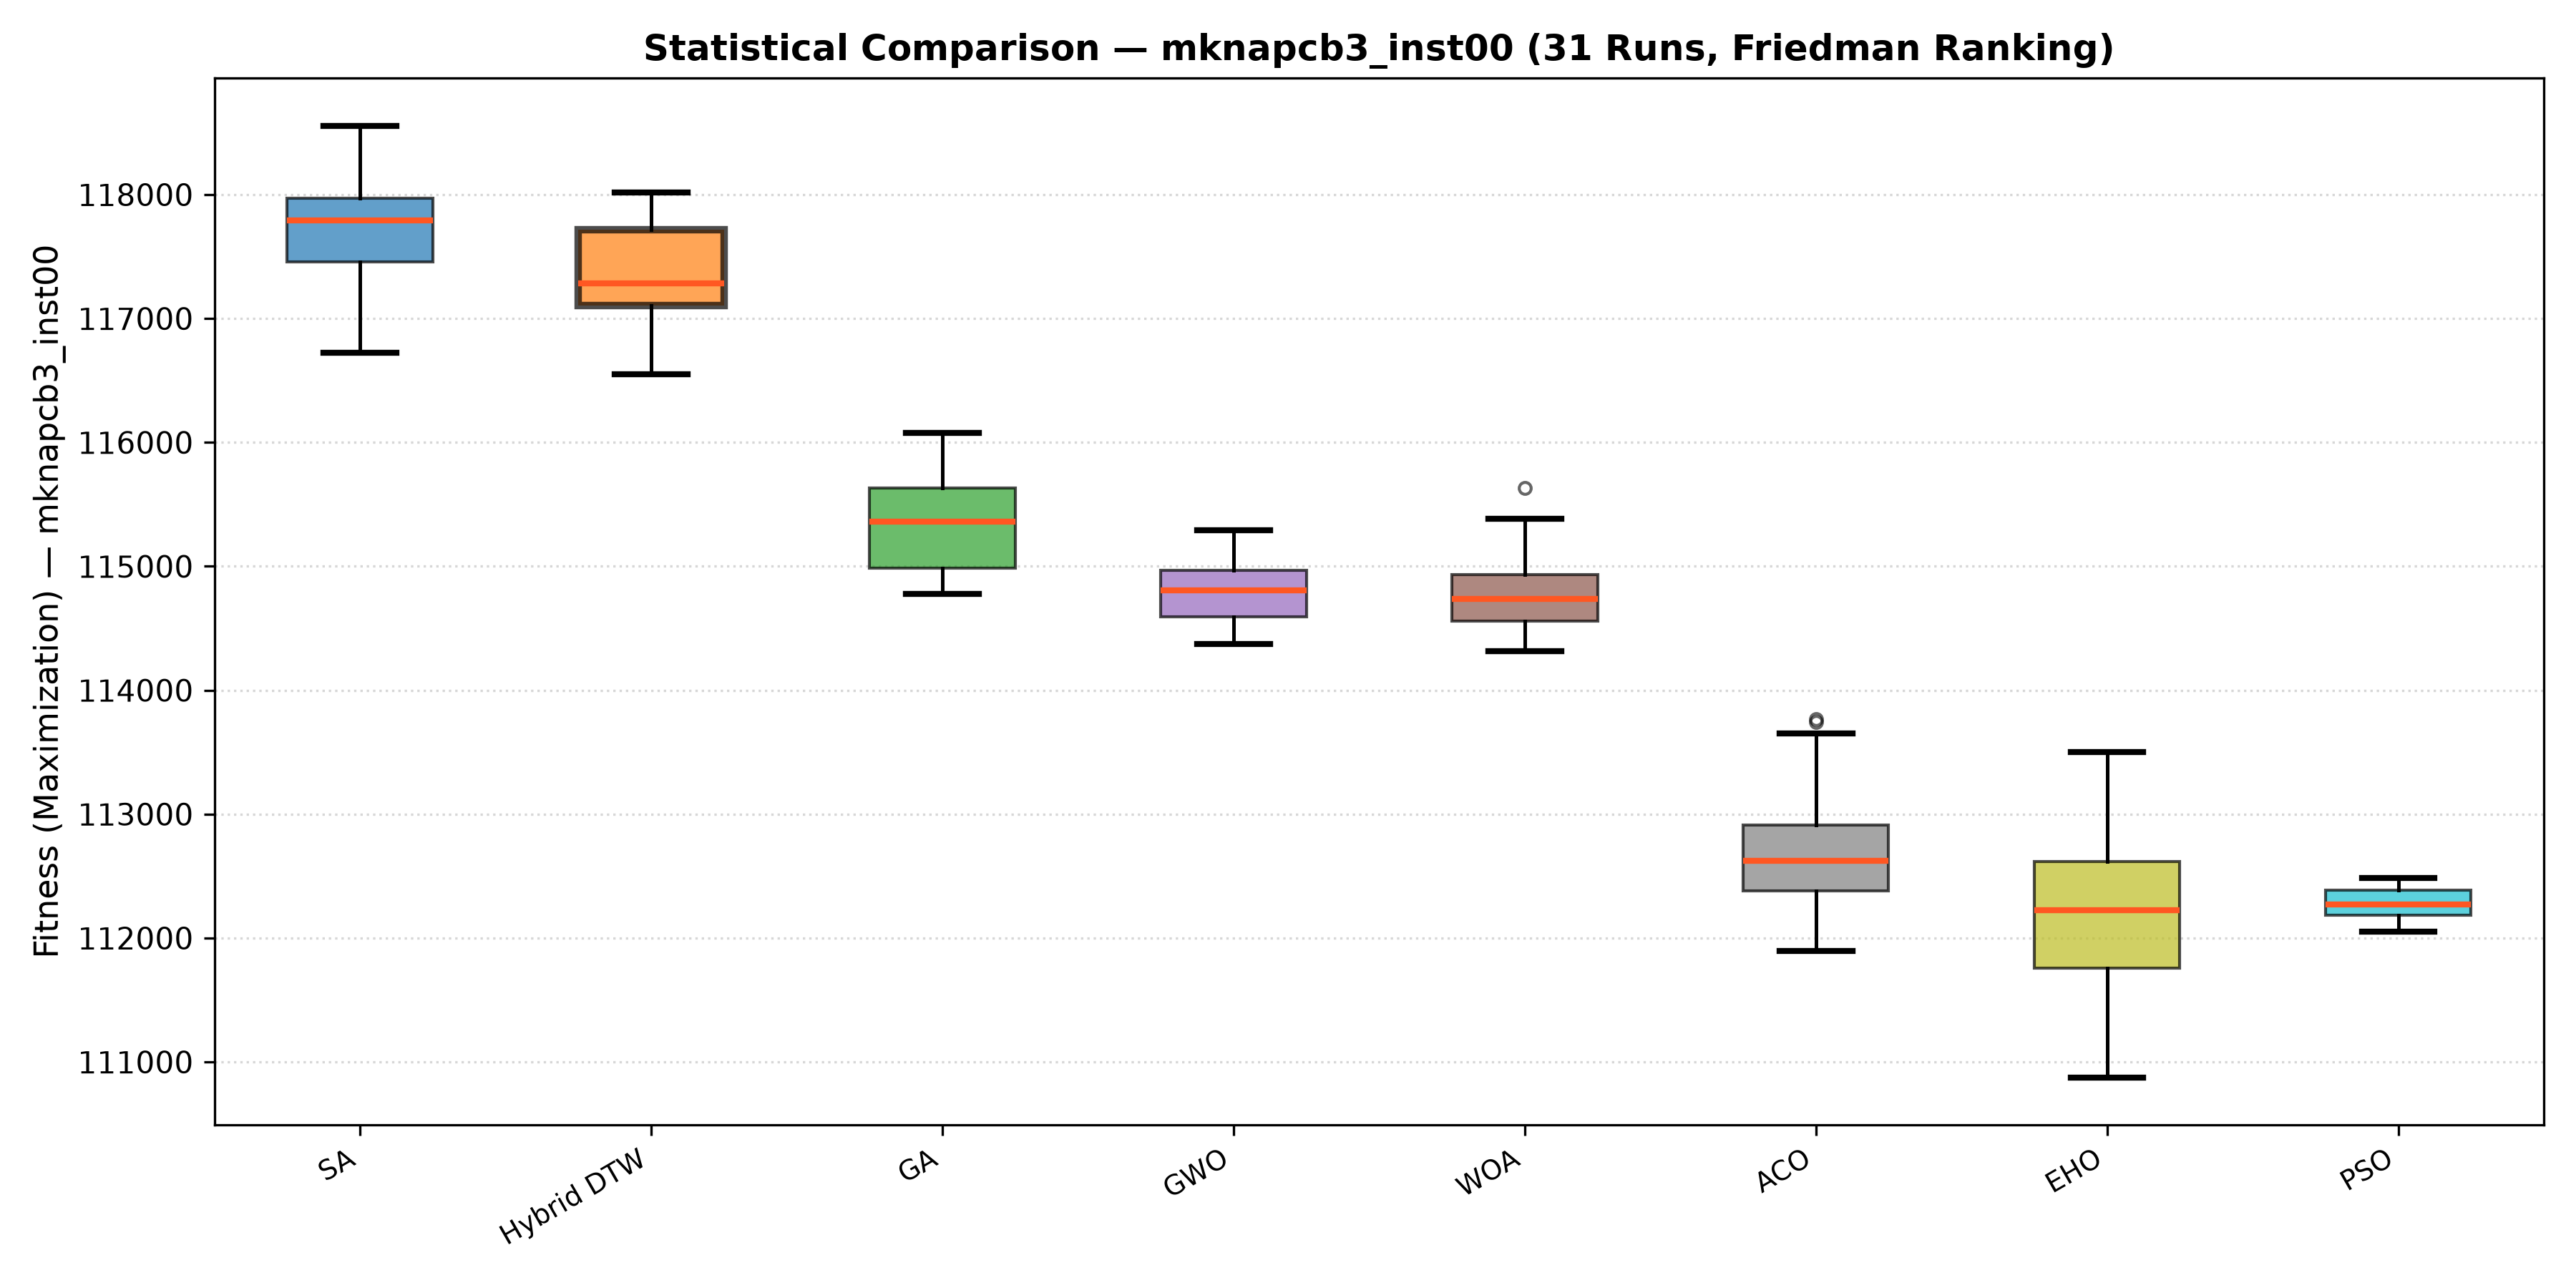
\includegraphics[width=0.32\textwidth]{imagenes_paper/mkp_dtw_3k_mknapcb3_comparativo_mh.png}}\hfill
\subfloat[Best-run convergence.]{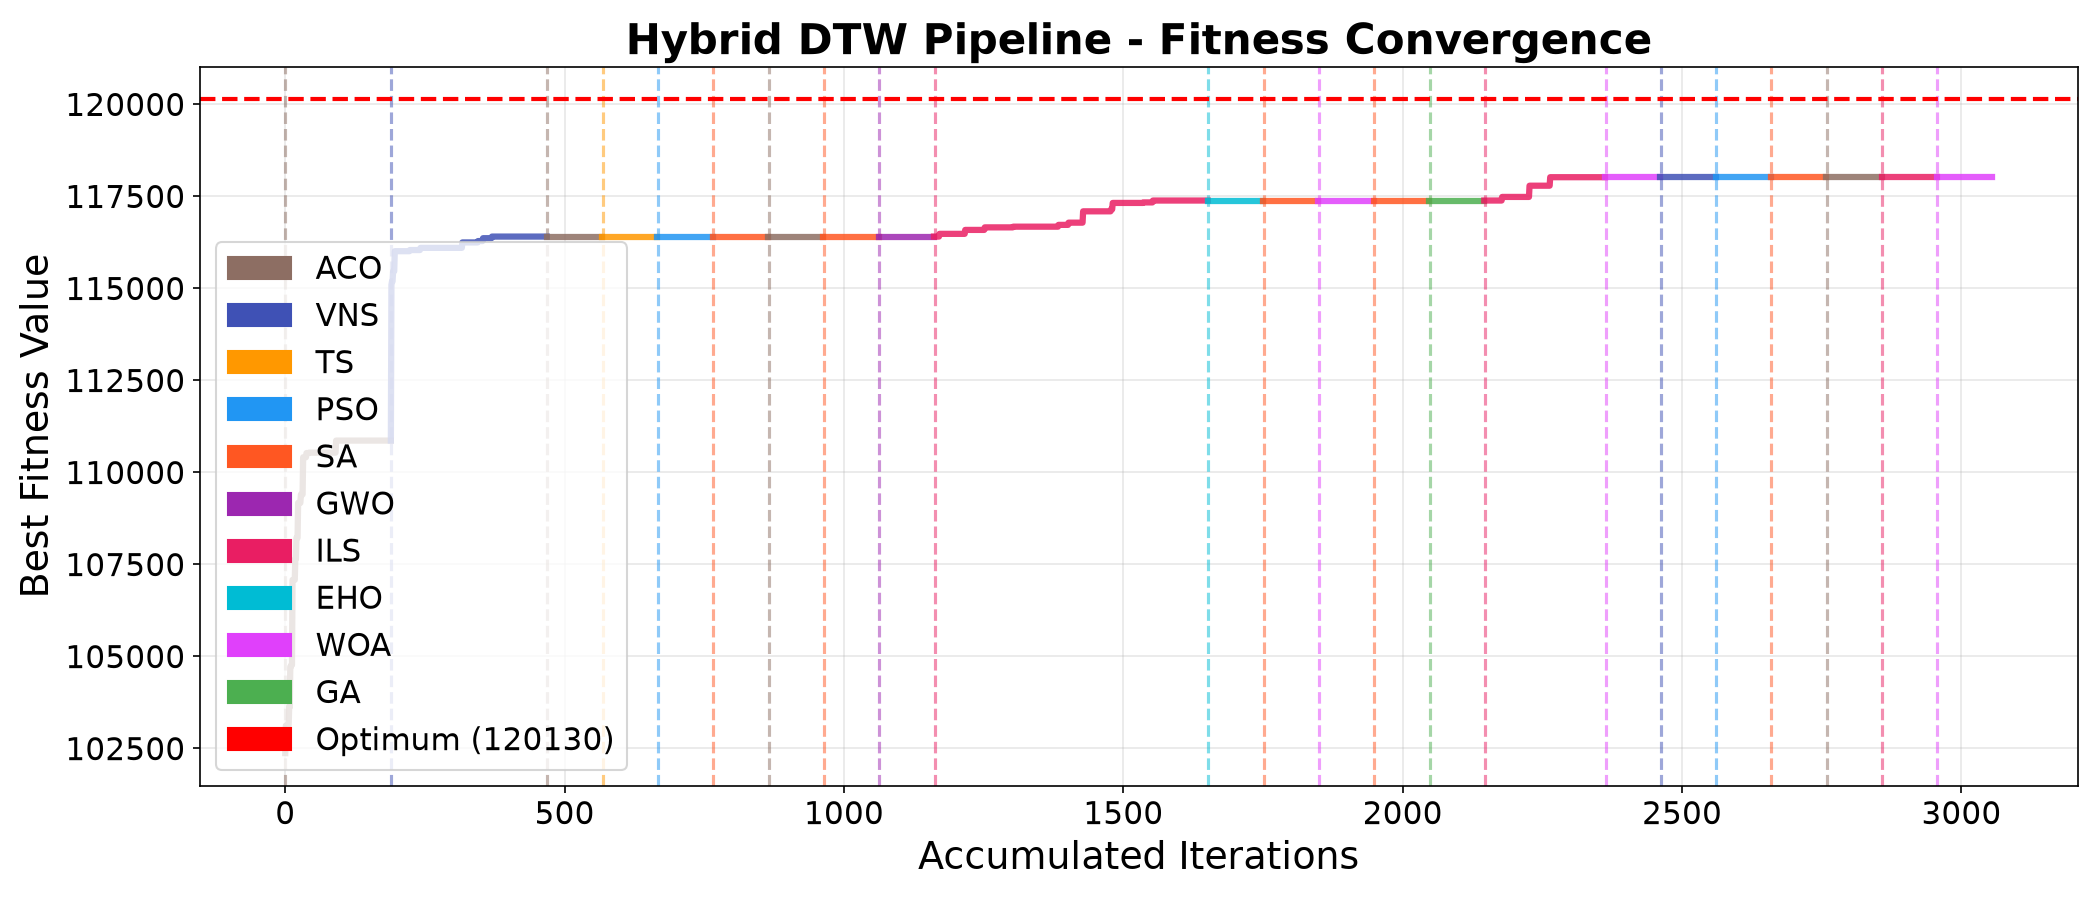
\includegraphics[width=0.32\textwidth]{imagenes_paper/mkp_dtw_3k_mknapcb3_convergencia.png}}\hfill
\subfloat[Elastic metric $\Delta=D_1-D_2$.]{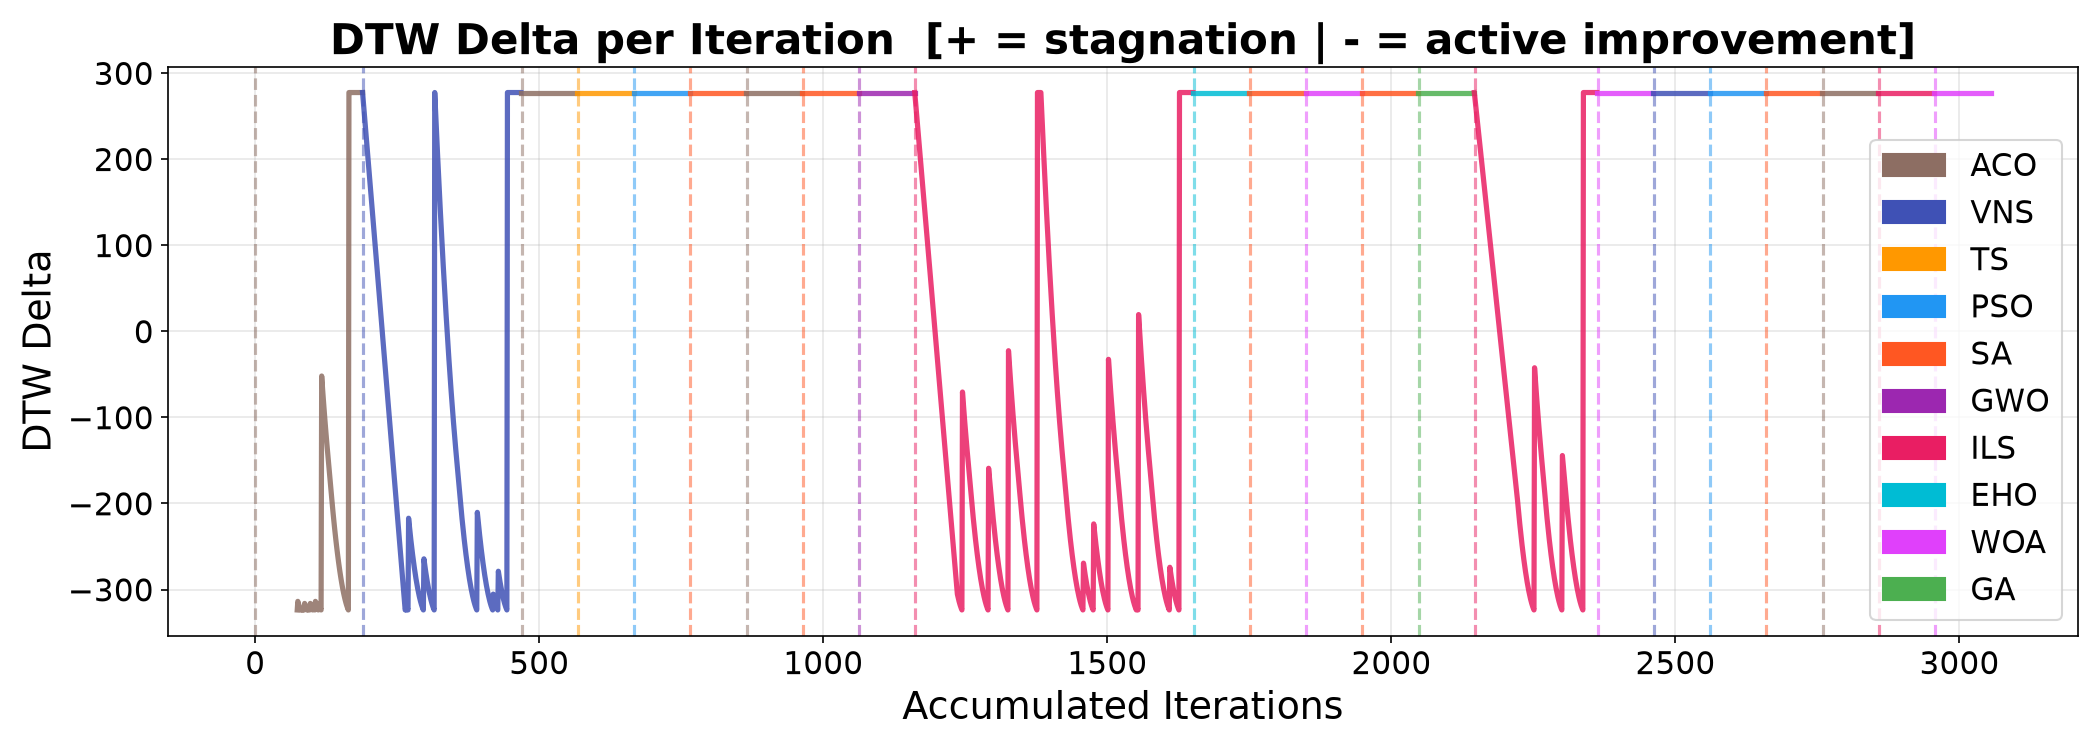
\includegraphics[width=0.32\textwidth]{imagenes_paper/mkp_dtw_3k_mknapcb3_delta.png}}
\caption{Diagnostic suite for instance \textbf{mknapcb3} ($n=500$, $m=5$) under the DTW framework with $T_{\max}=3{,}000$: (a)~final-fitness distribution over $N=31$ runs; (b)~convergence trajectory of the best run; (c)~elastic warping profile $\Delta$.}
\label{fig:mkp-best-cb3}
\end{figure}

% --- mknapcb4: DTW, 3,000 iterations ---
\begin{figure}[htbp]
\centering
\subfloat[Metaheuristic comparison.]{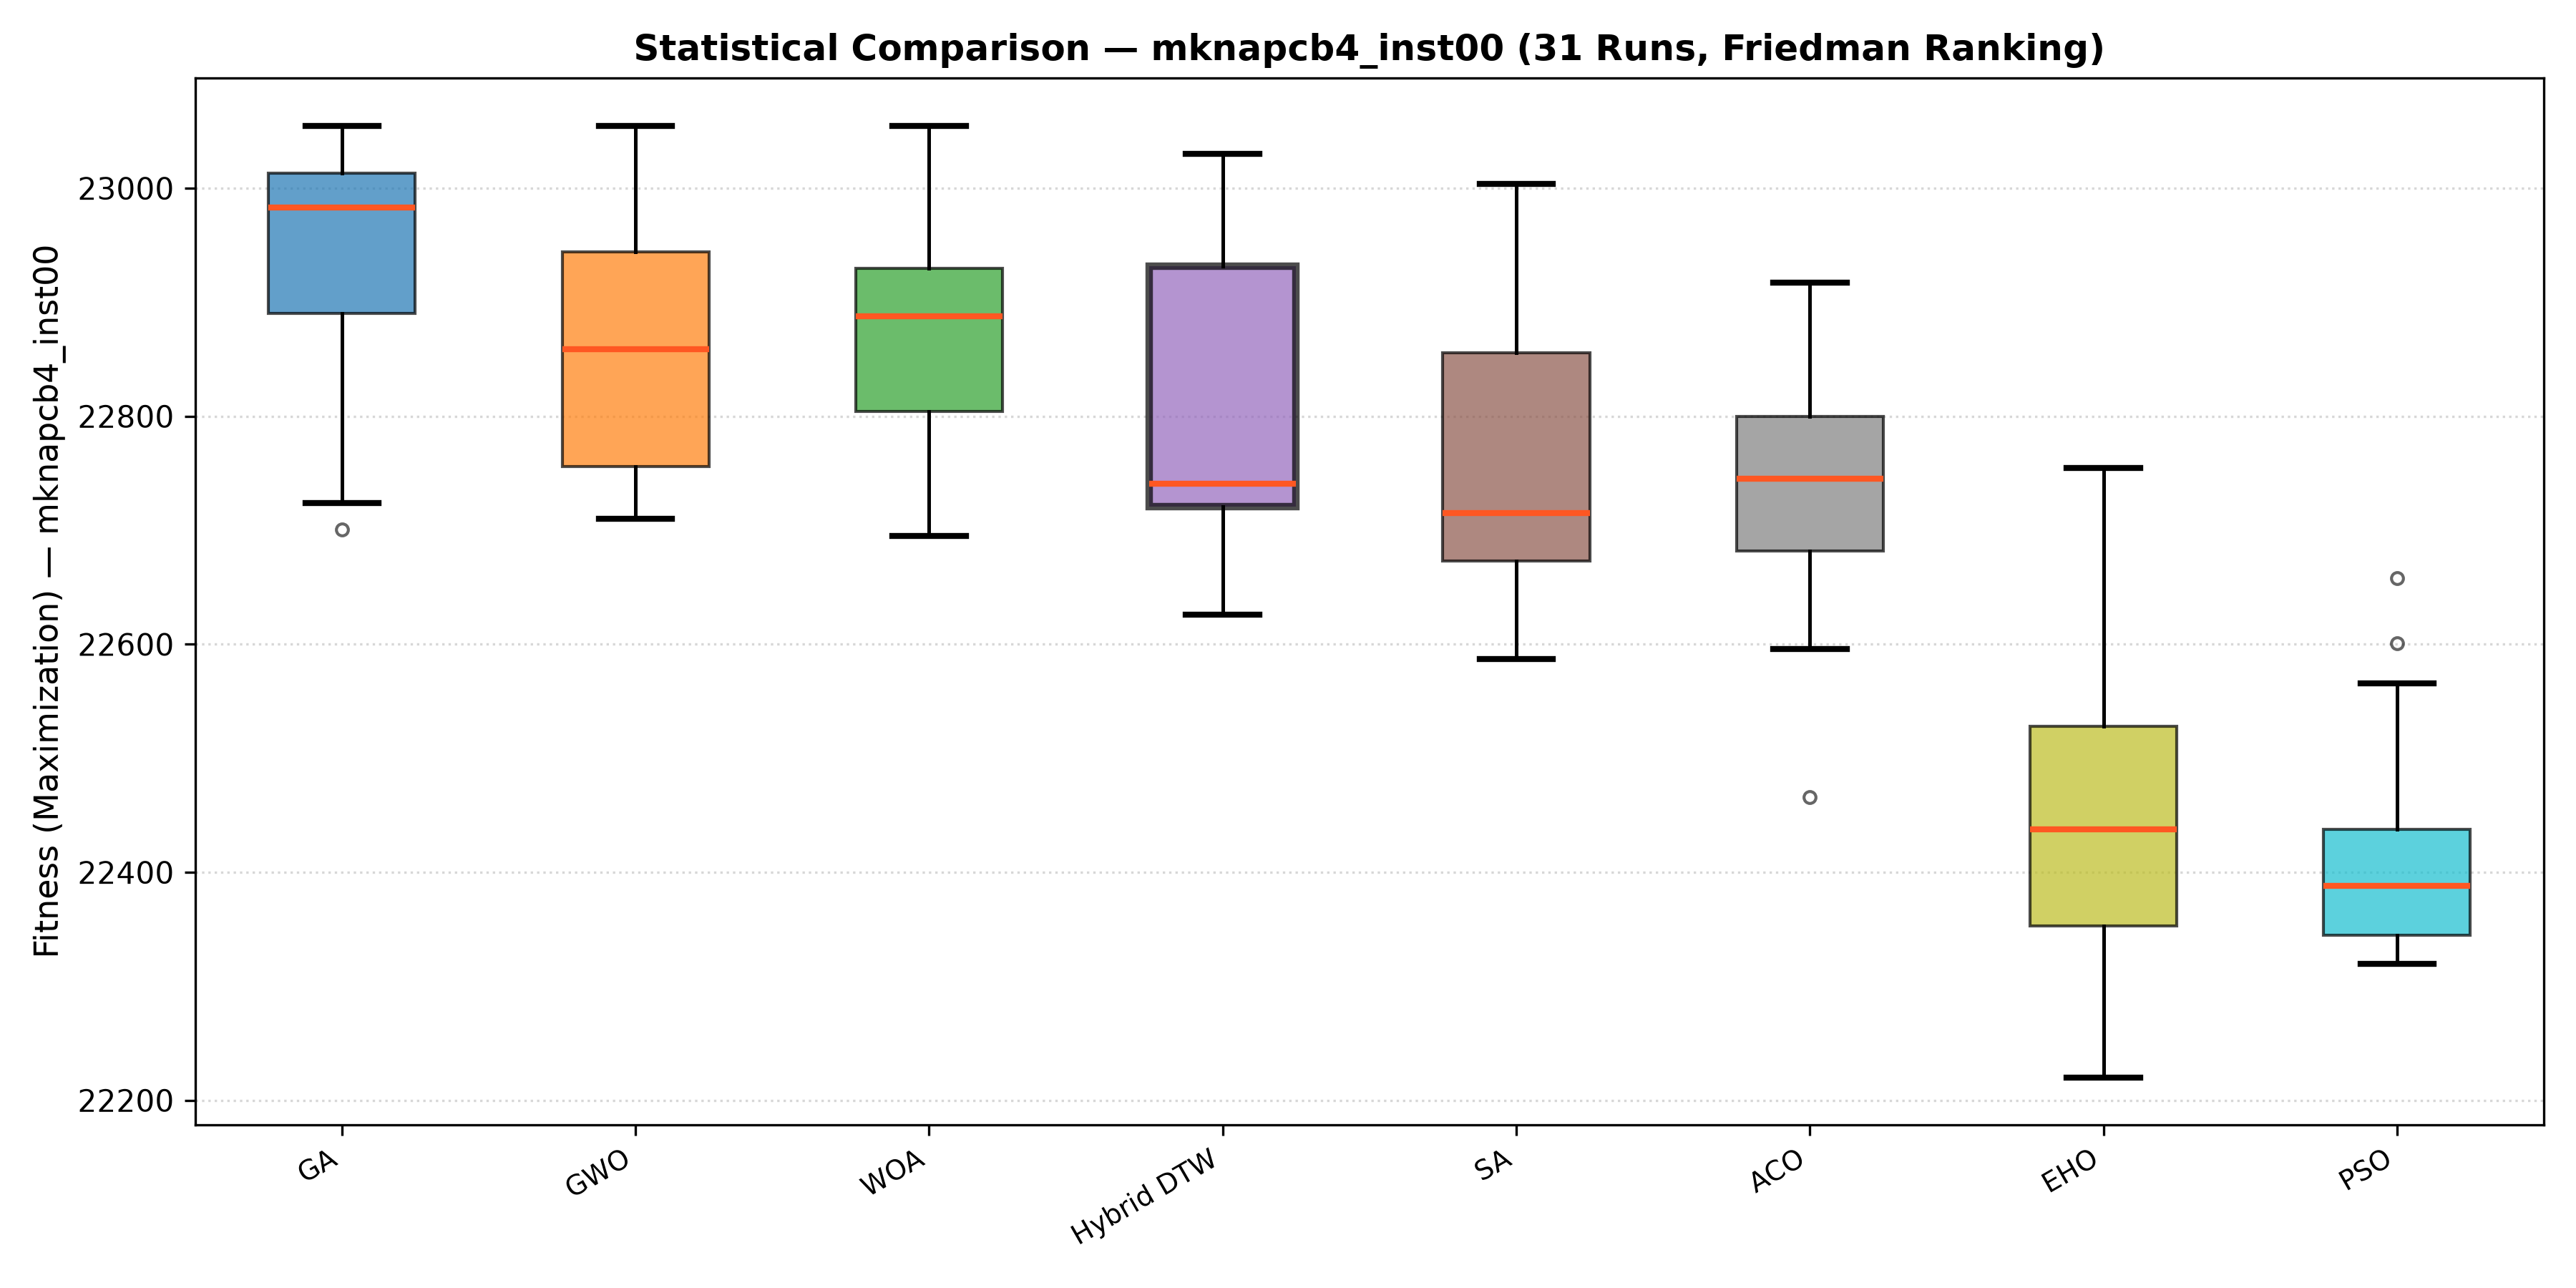
\includegraphics[width=0.32\textwidth]{imagenes_paper/mkp_dtw_3k_mknapcb4_comparativo_mh.png}}\hfill
\subfloat[Best-run convergence.]{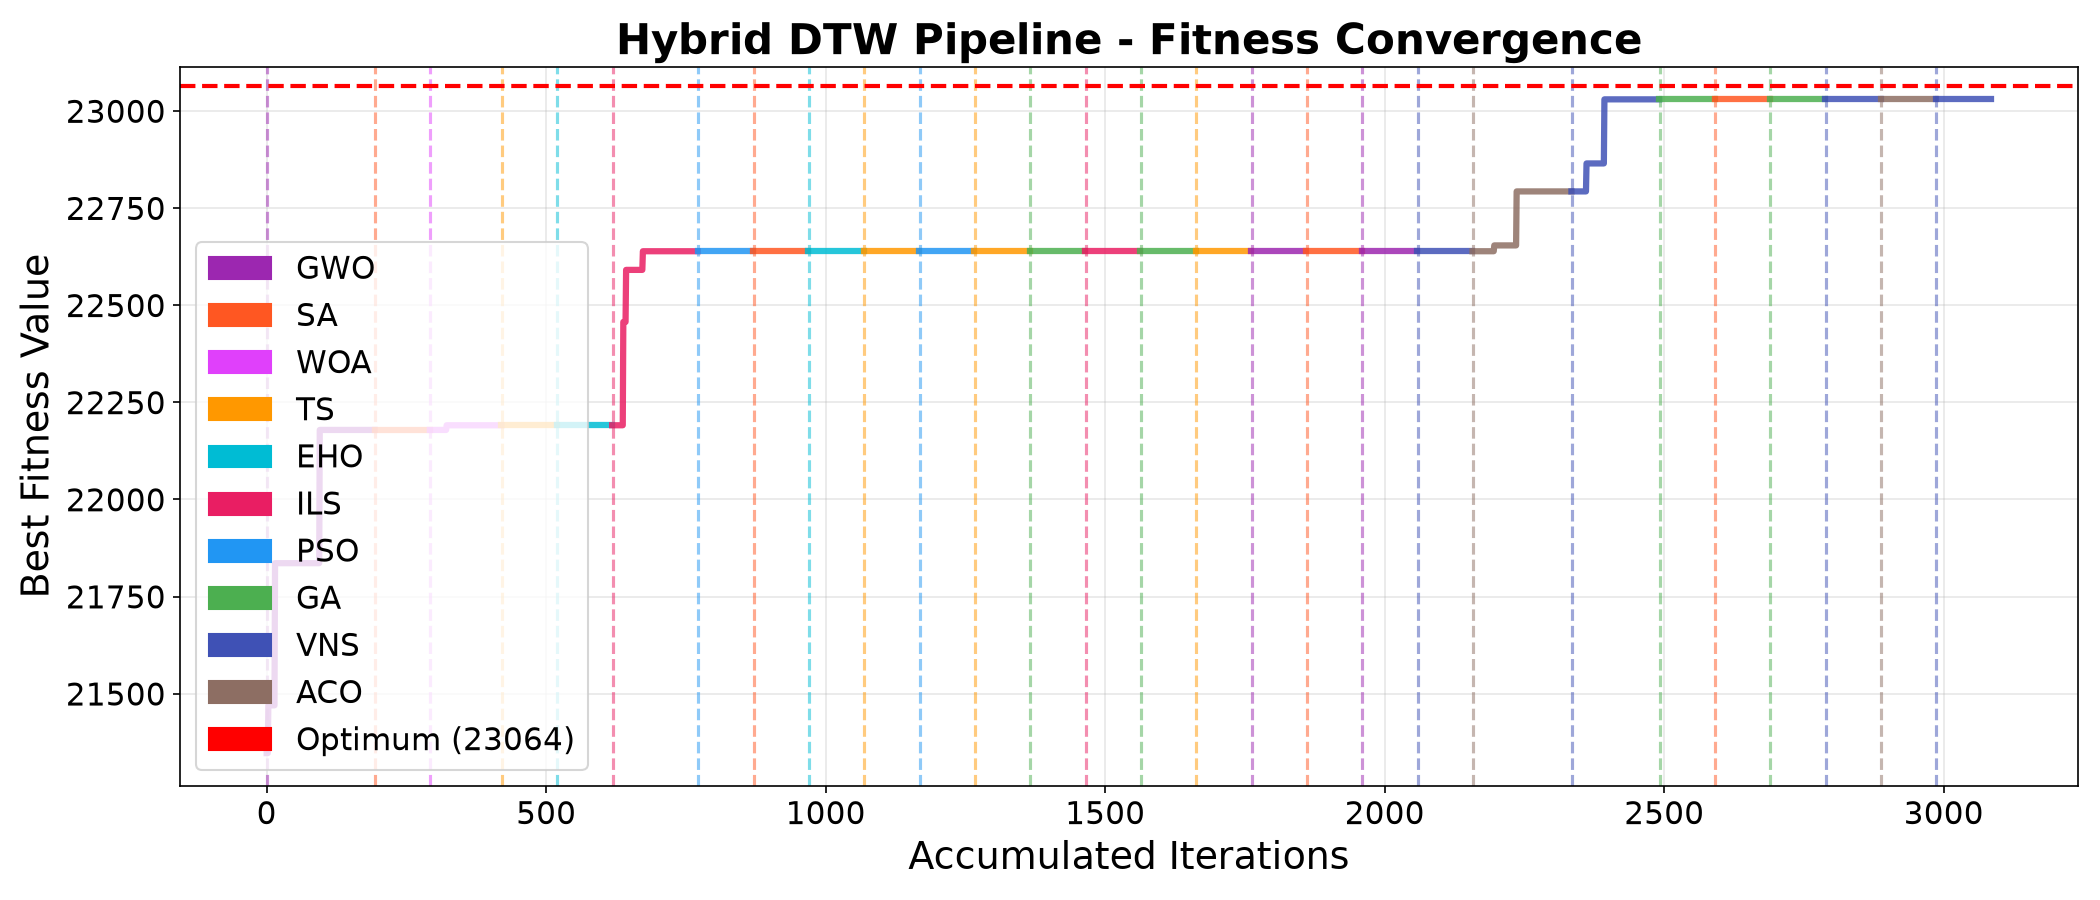
\includegraphics[width=0.32\textwidth]{imagenes_paper/mkp_dtw_3k_mknapcb4_convergencia.png}}\hfill
\subfloat[Elastic metric $\Delta=D_1-D_2$.]{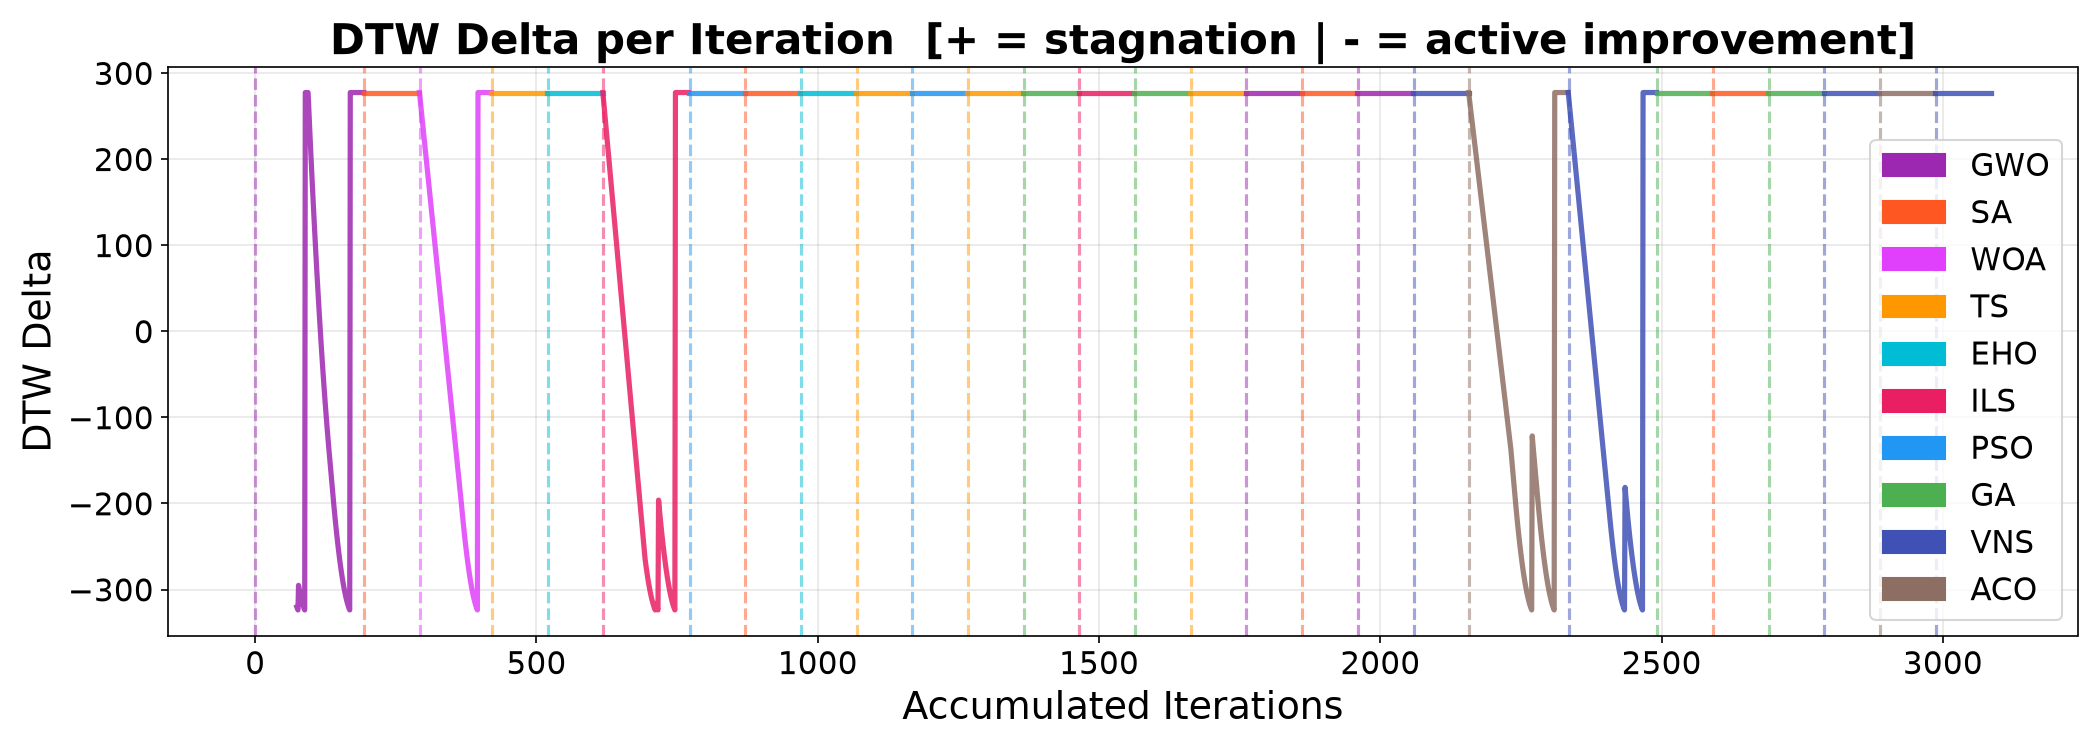
\includegraphics[width=0.32\textwidth]{imagenes_paper/mkp_dtw_3k_mknapcb4_delta.png}}
\caption{Diagnostic suite for instance \textbf{mknapcb4} ($n=100$, $m=10$) under the DTW framework with $T_{\max}=3{,}000$: (a)~final-fitness distribution over $N=31$ runs; (b)~convergence trajectory of the best run; (c)~elastic warping profile $\Delta$.}
\label{fig:mkp-best-cb4}
\end{figure}

% --- mknapcb5: DTW, 3,000 iterations ---
\begin{figure}[htbp]
\centering
\subfloat[Metaheuristic comparison.]{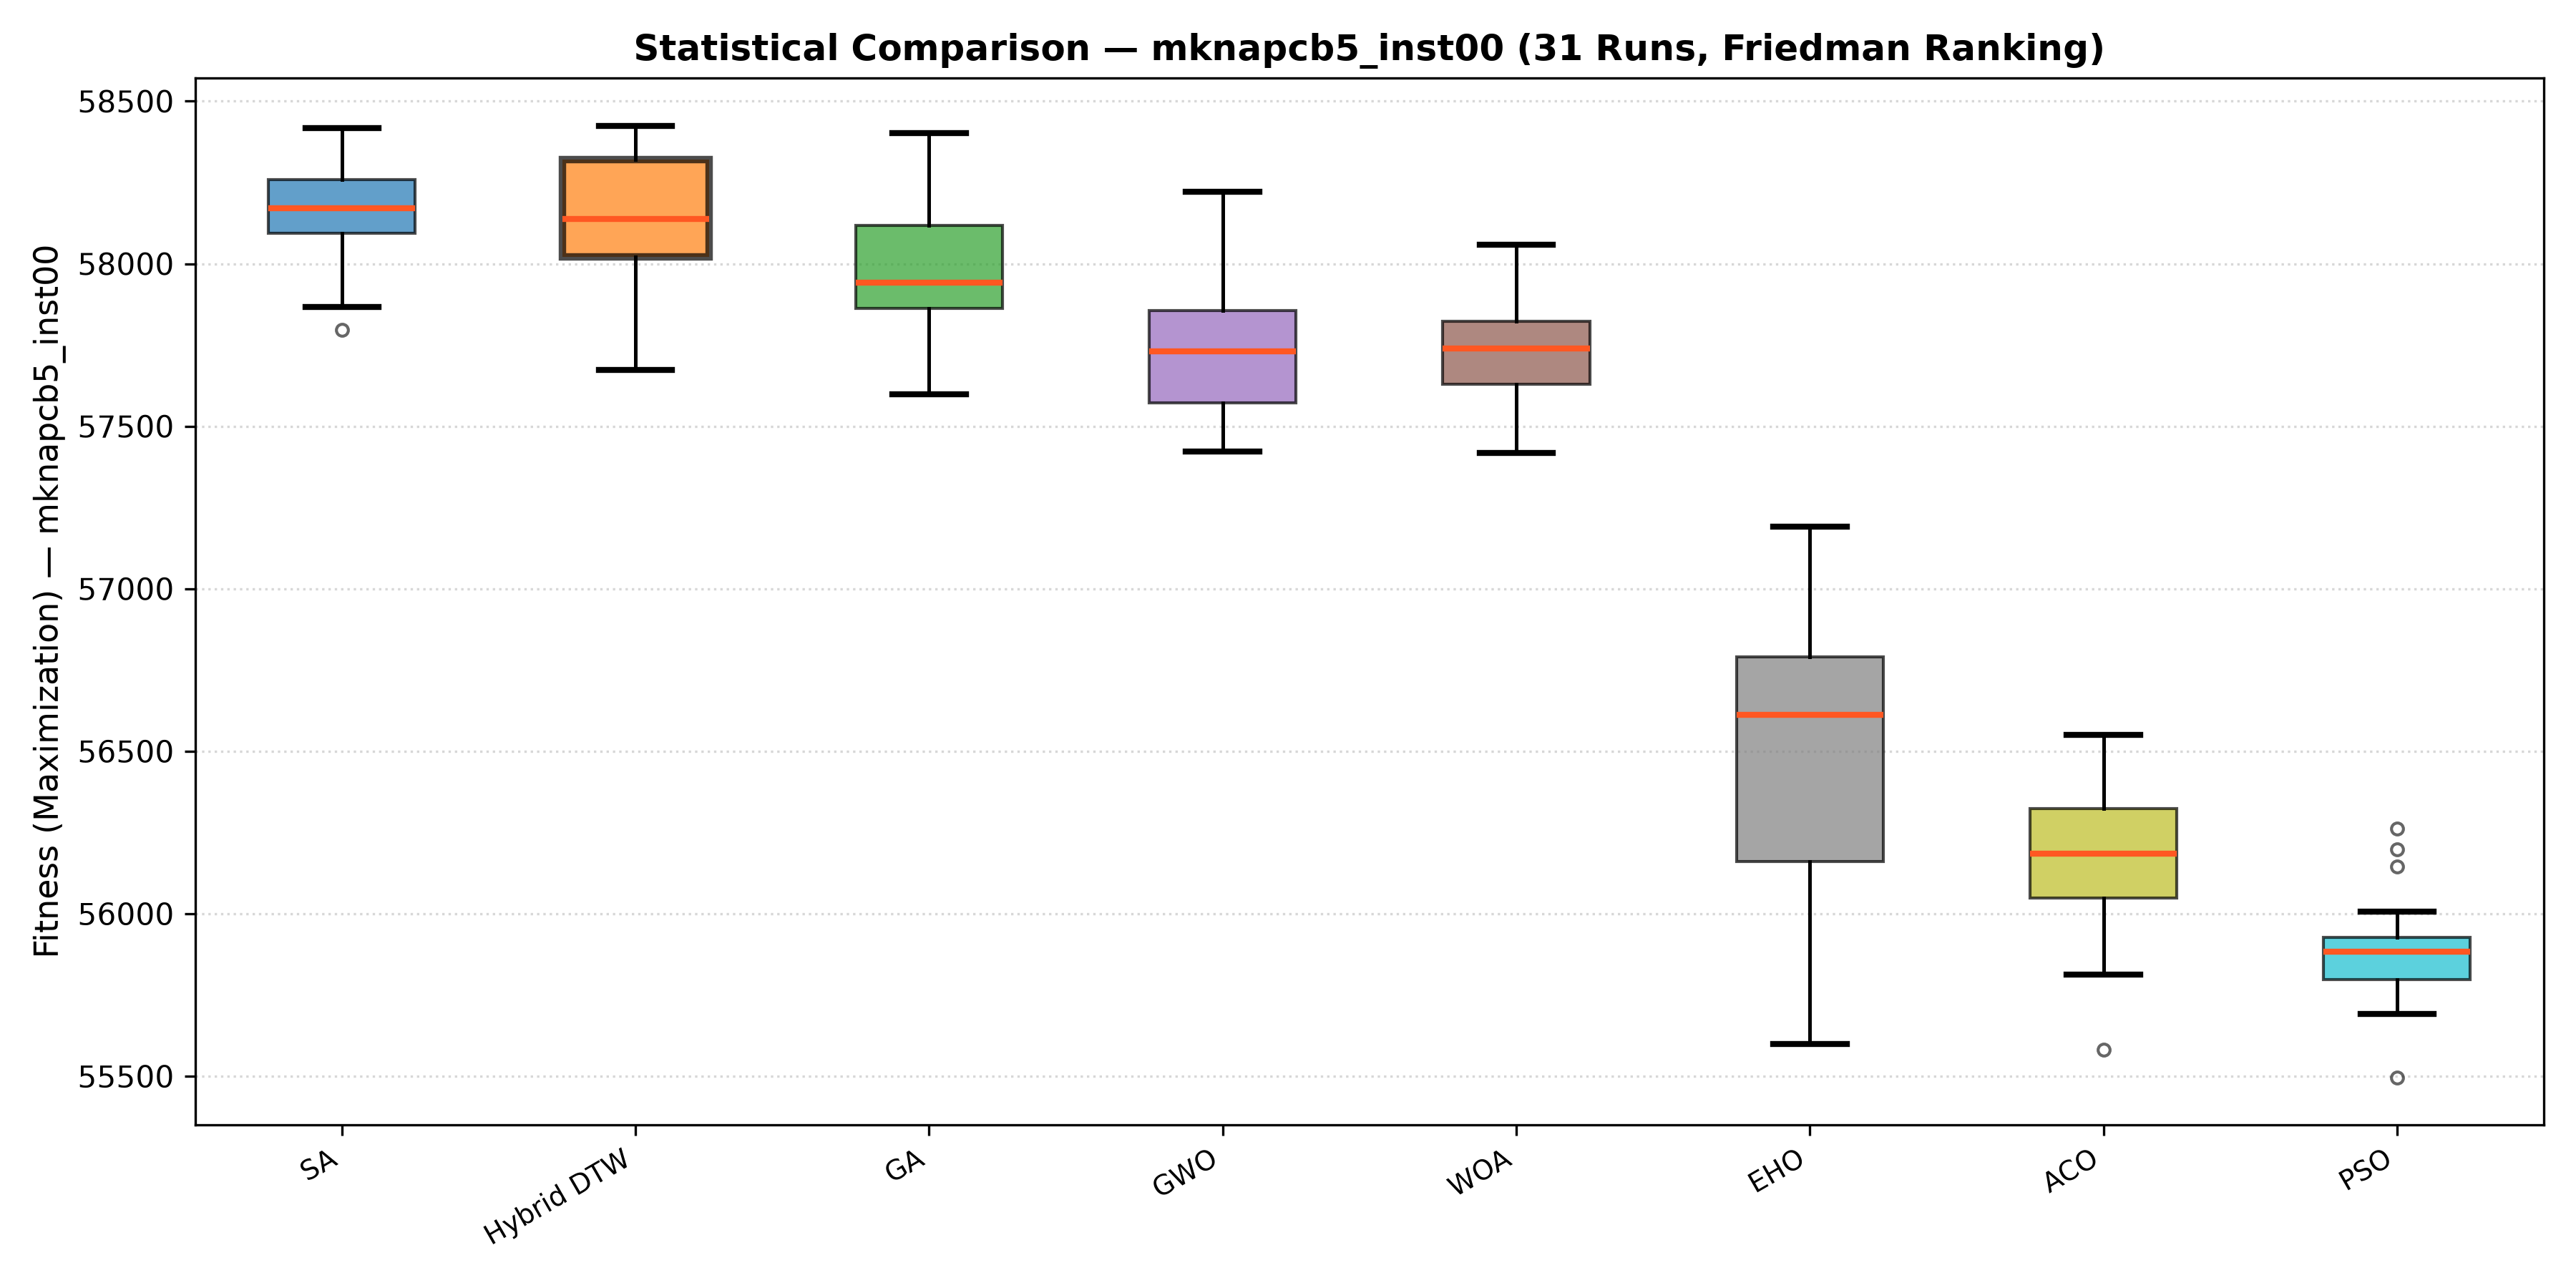
\includegraphics[width=0.32\textwidth]{imagenes_paper/mkp_dtw_3k_mknapcb5_comparativo_mh.png}}\hfill
\subfloat[Best-run convergence.]{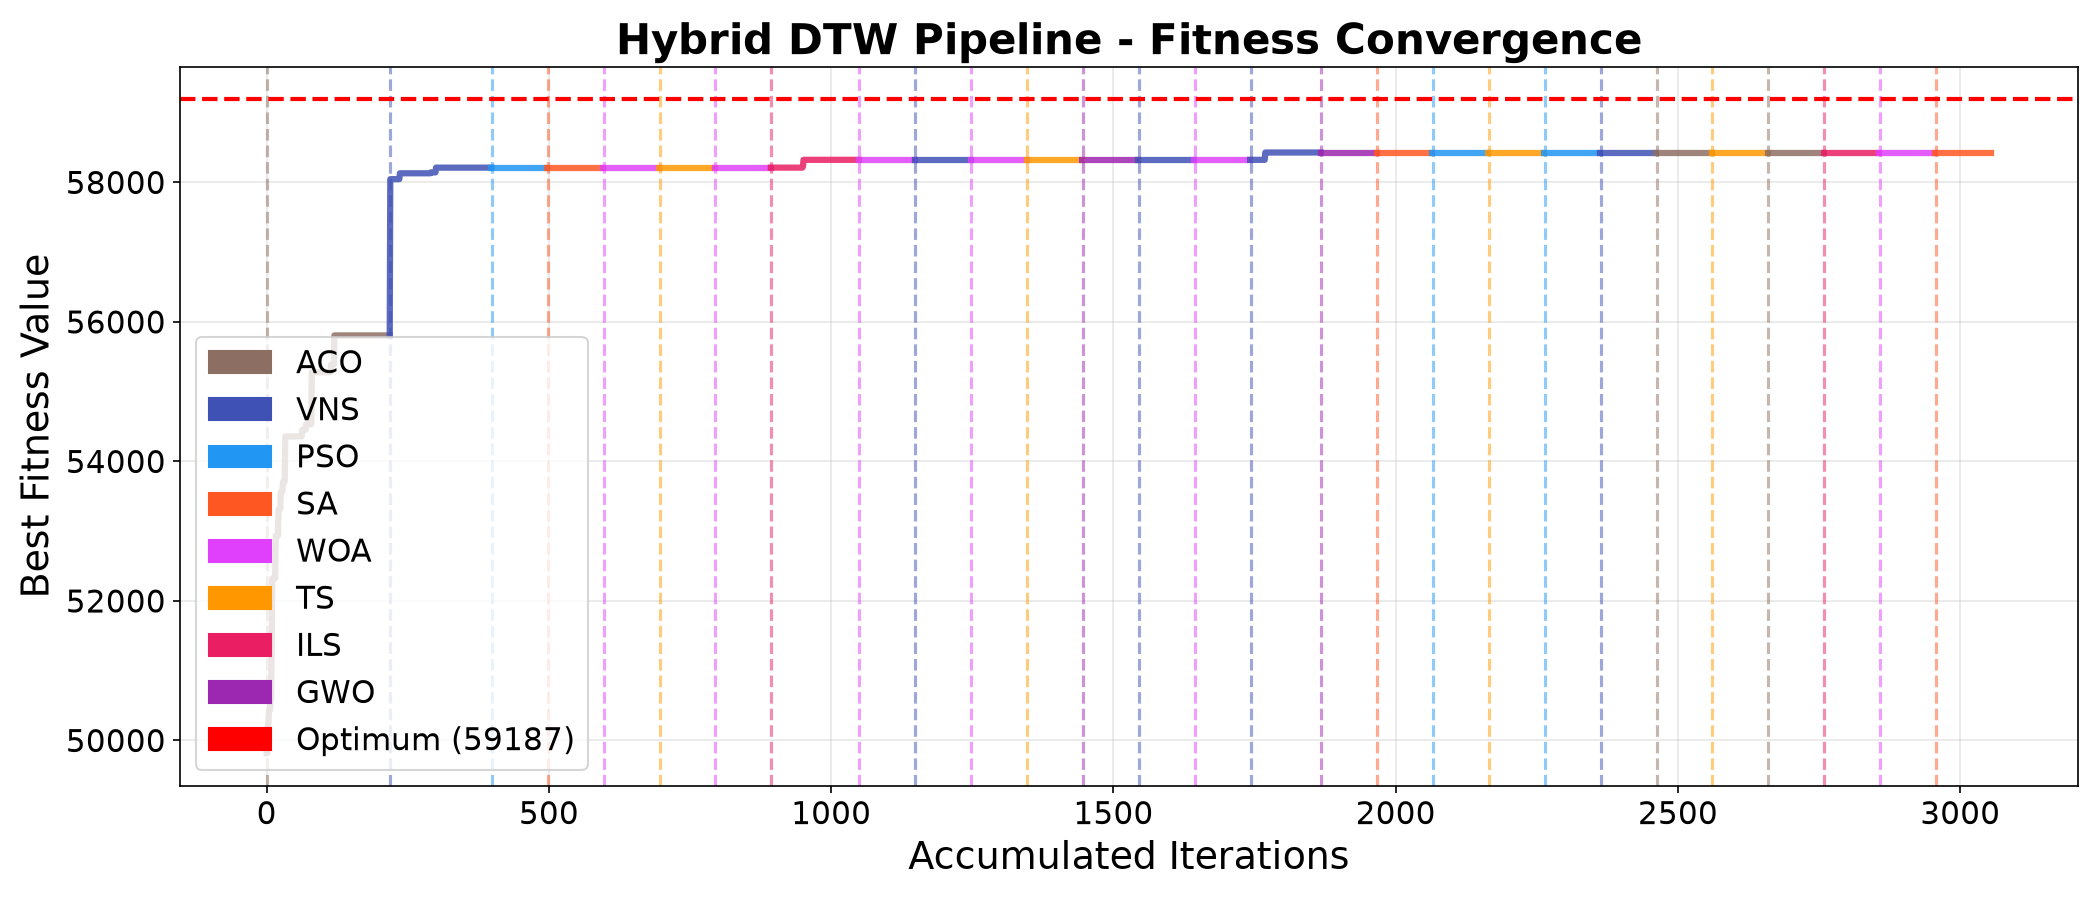
\includegraphics[width=0.32\textwidth]{imagenes_paper/mkp_dtw_3k_mknapcb5_convergencia.png}}\hfill
\subfloat[Elastic metric $\Delta=D_1-D_2$.]{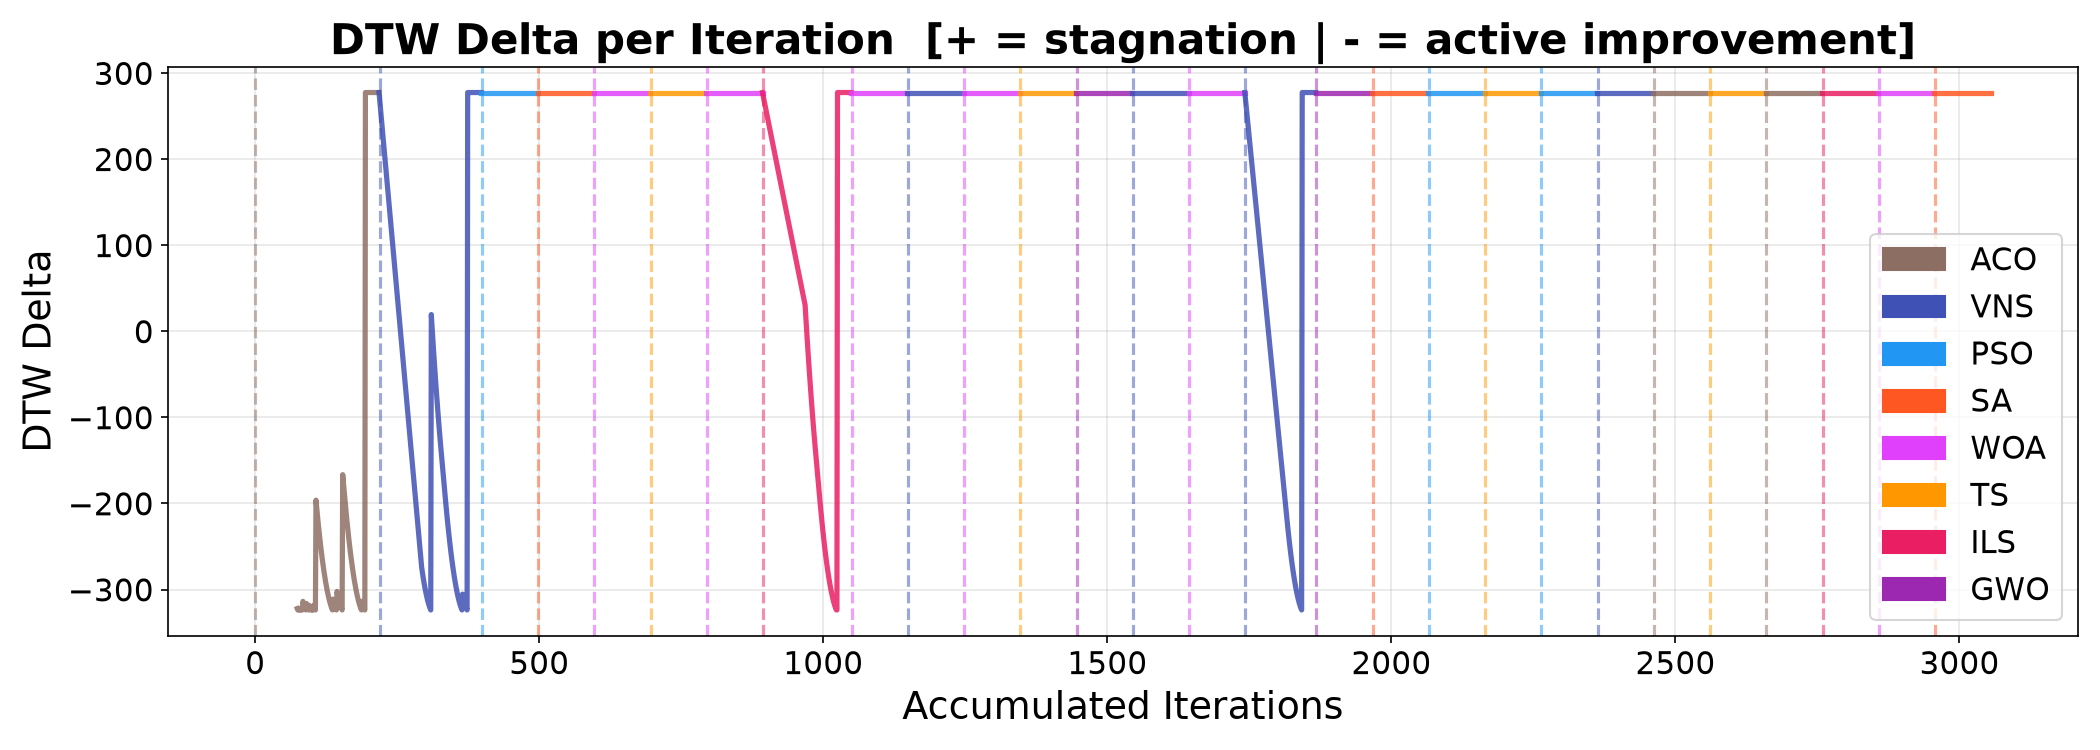
\includegraphics[width=0.32\textwidth]{imagenes_paper/mkp_dtw_3k_mknapcb5_delta.png}}
\caption{Diagnostic suite for instance \textbf{mknapcb5} ($n=250$, $m=10$) under the DTW framework with $T_{\max}=3{,}000$: (a)~final-fitness distribution over $N=31$ runs; (b)~convergence trajectory of the best run; (c)~elastic warping profile $\Delta$.}
\label{fig:mkp-best-cb5}
\end{figure}

% --- mknapcb6: DTW, 3,000 iterations ---
\begin{figure}[htbp]
\centering
\subfloat[Metaheuristic comparison.]{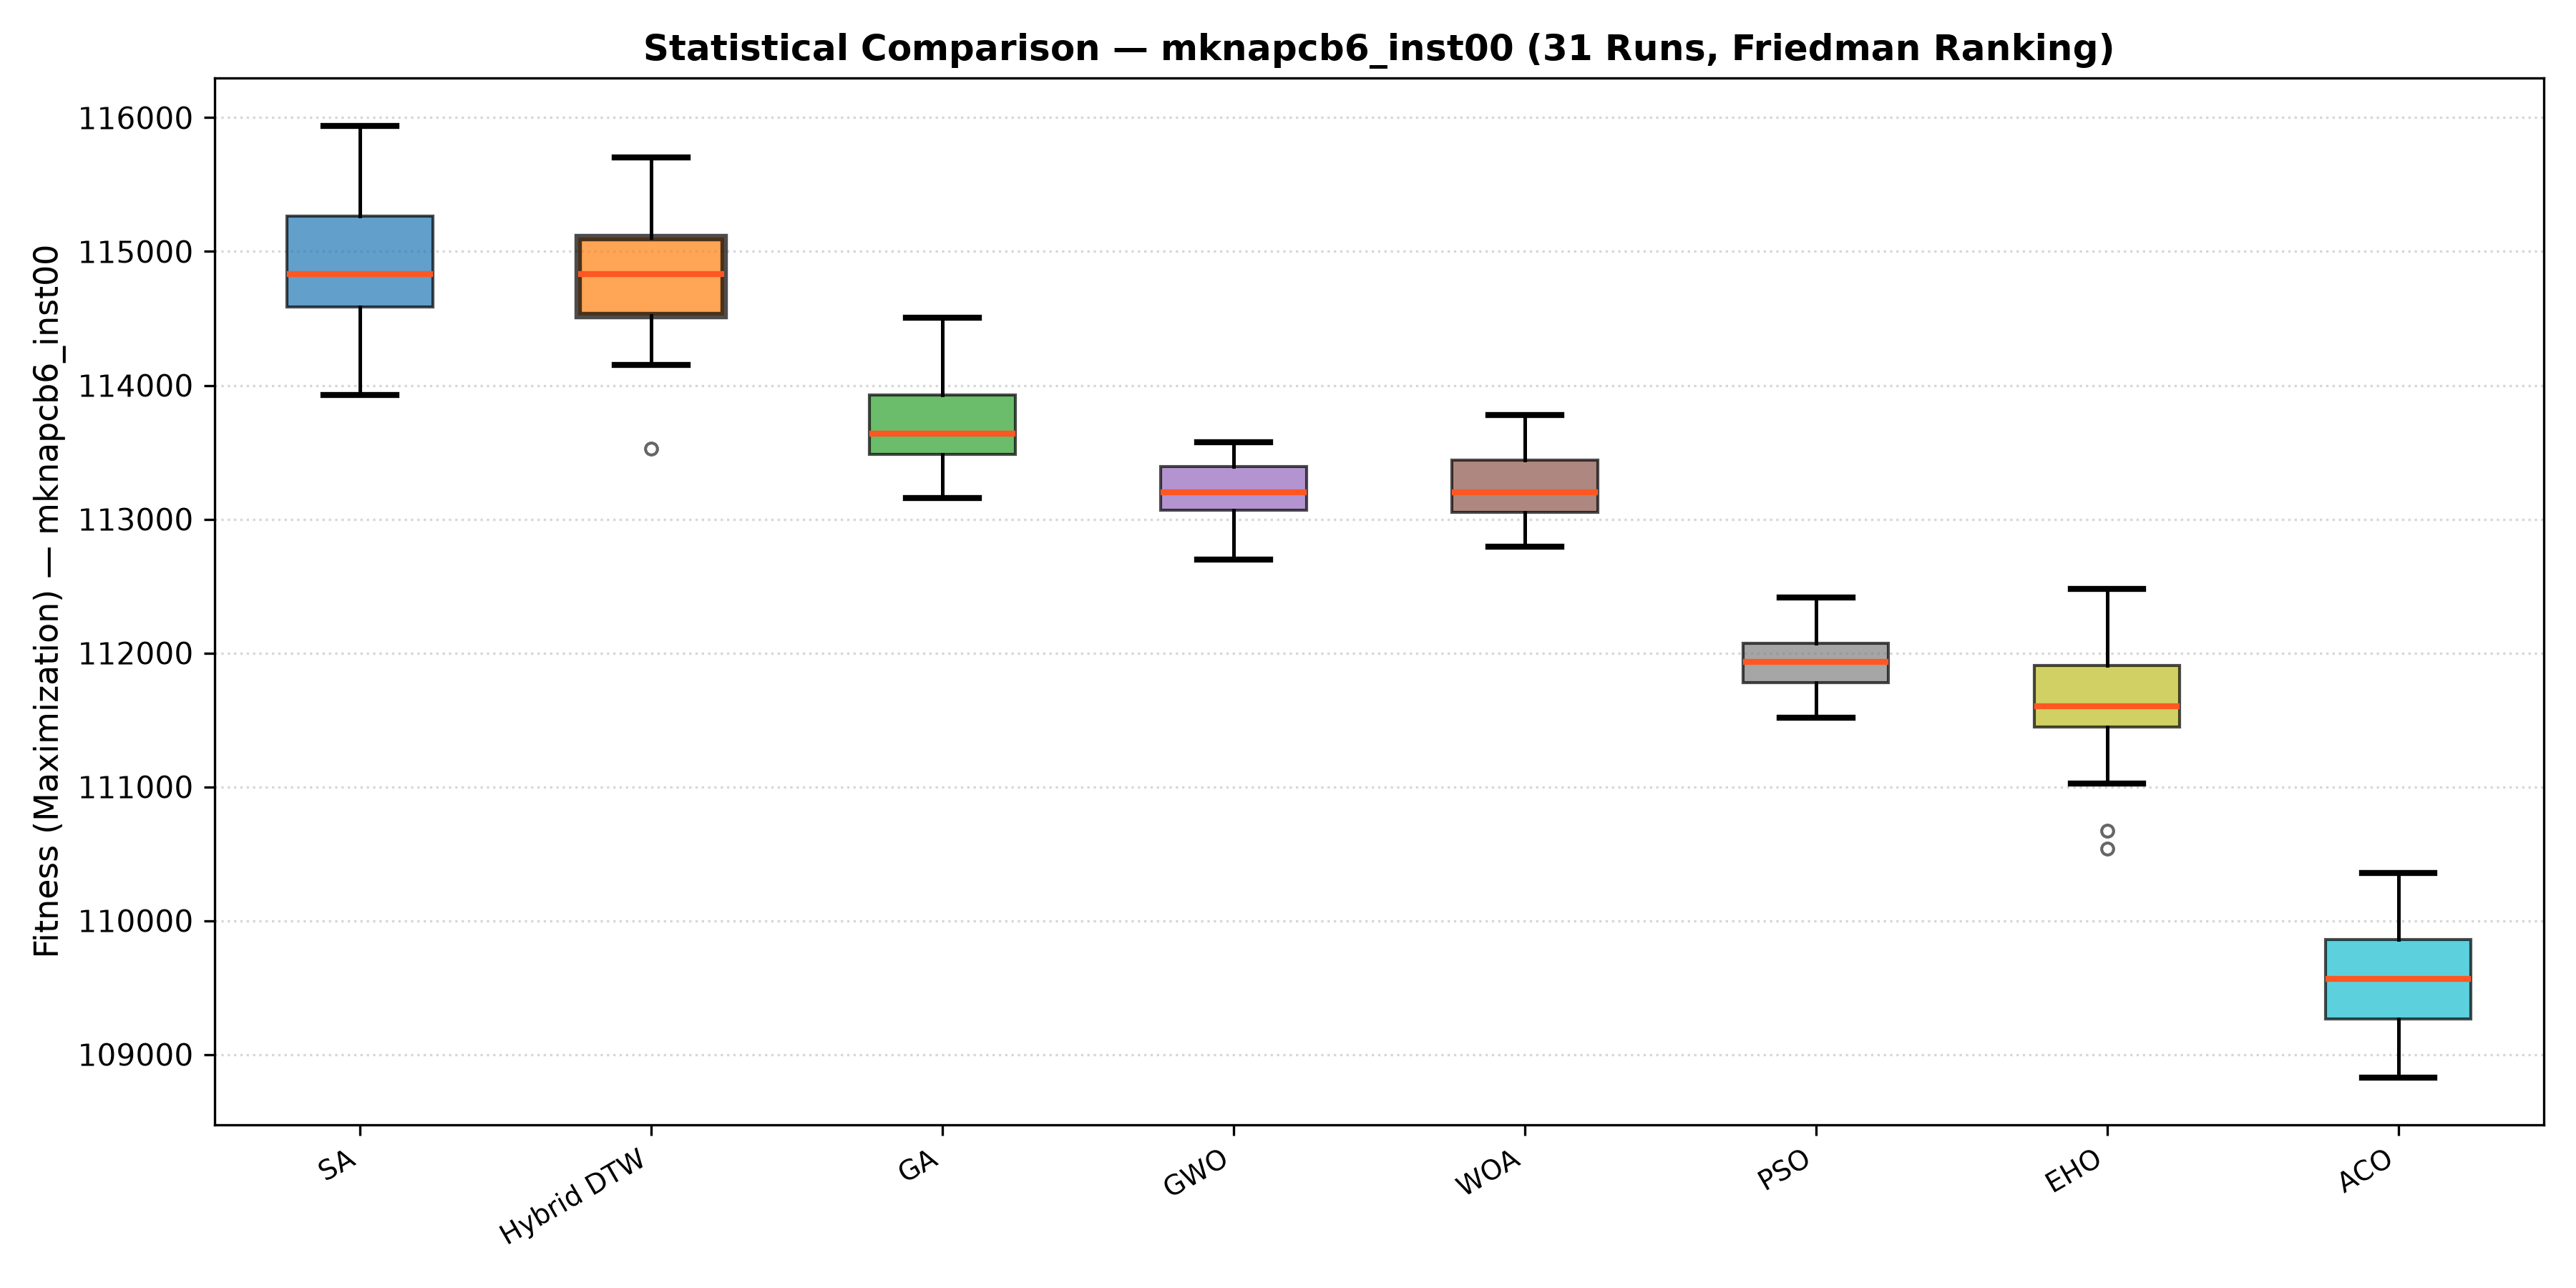
\includegraphics[width=0.32\textwidth]{imagenes_paper/mkp_dtw_3k_mknapcb6_comparativo_mh.png}}\hfill
\subfloat[Best-run convergence.]{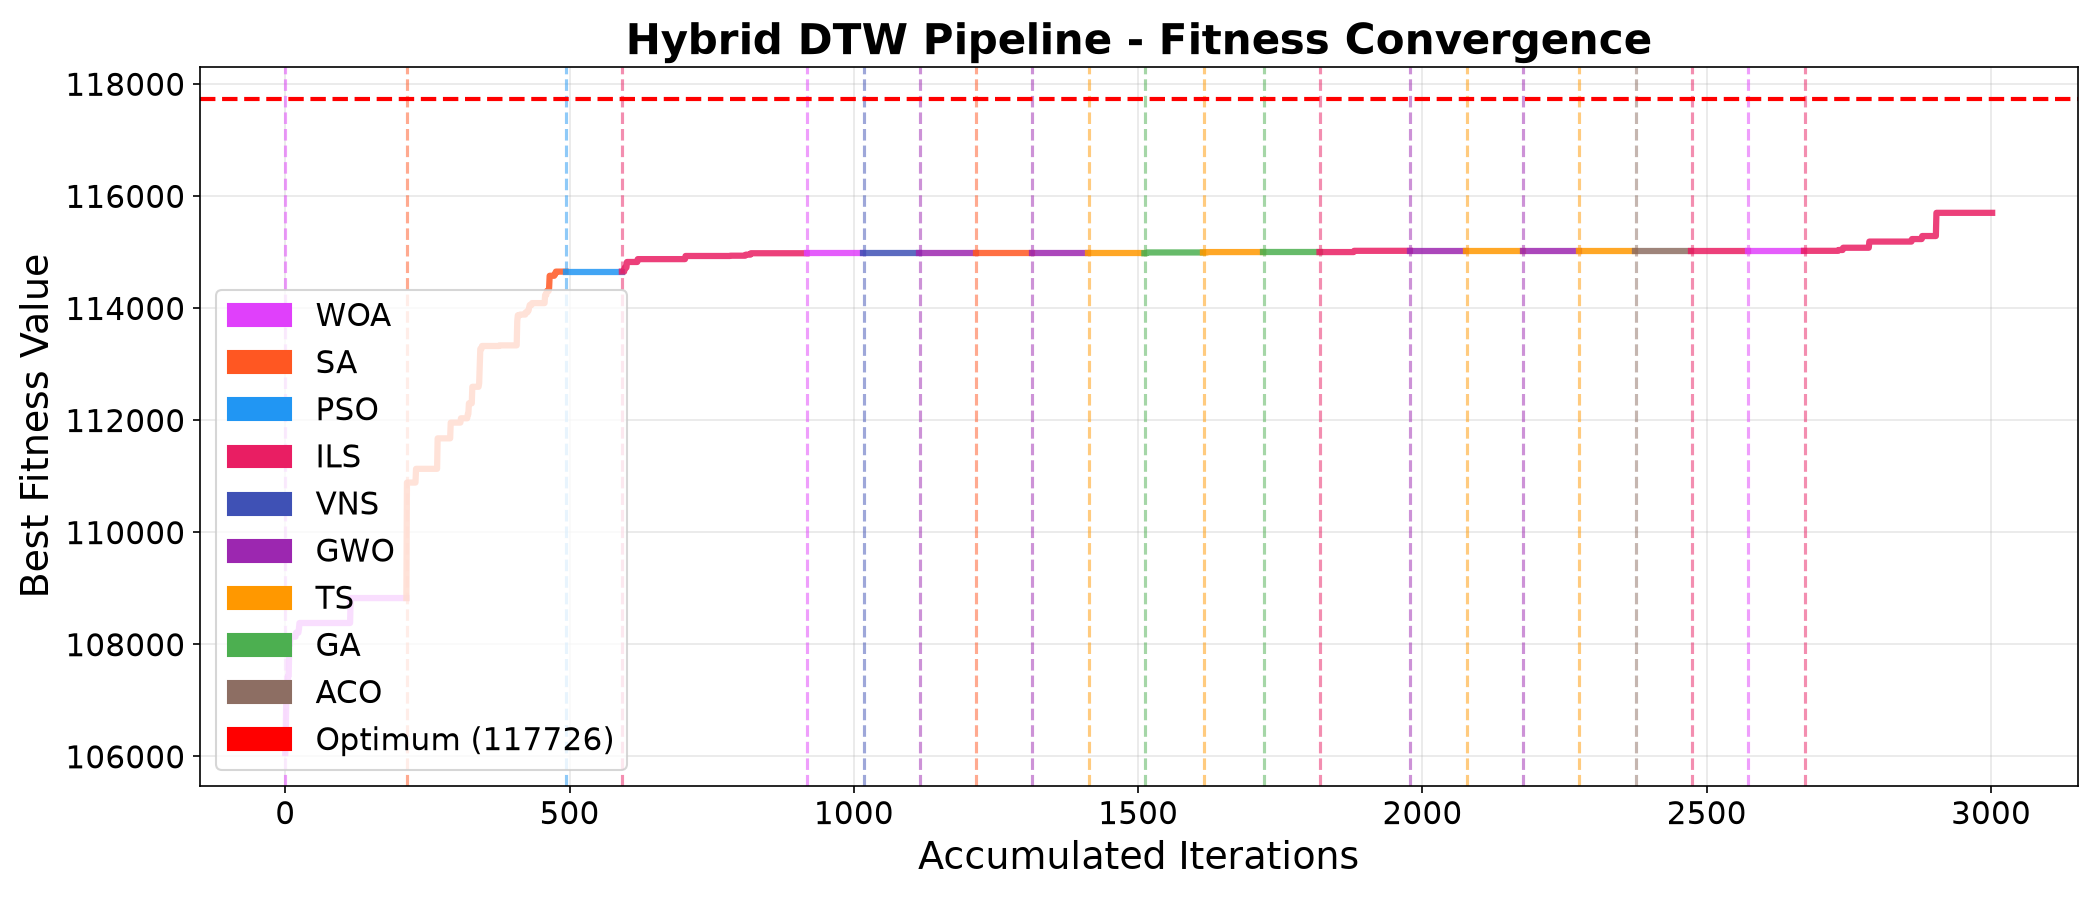
\includegraphics[width=0.32\textwidth]{imagenes_paper/mkp_dtw_3k_mknapcb6_convergencia.png}}\hfill
\subfloat[Elastic metric $\Delta=D_1-D_2$.]{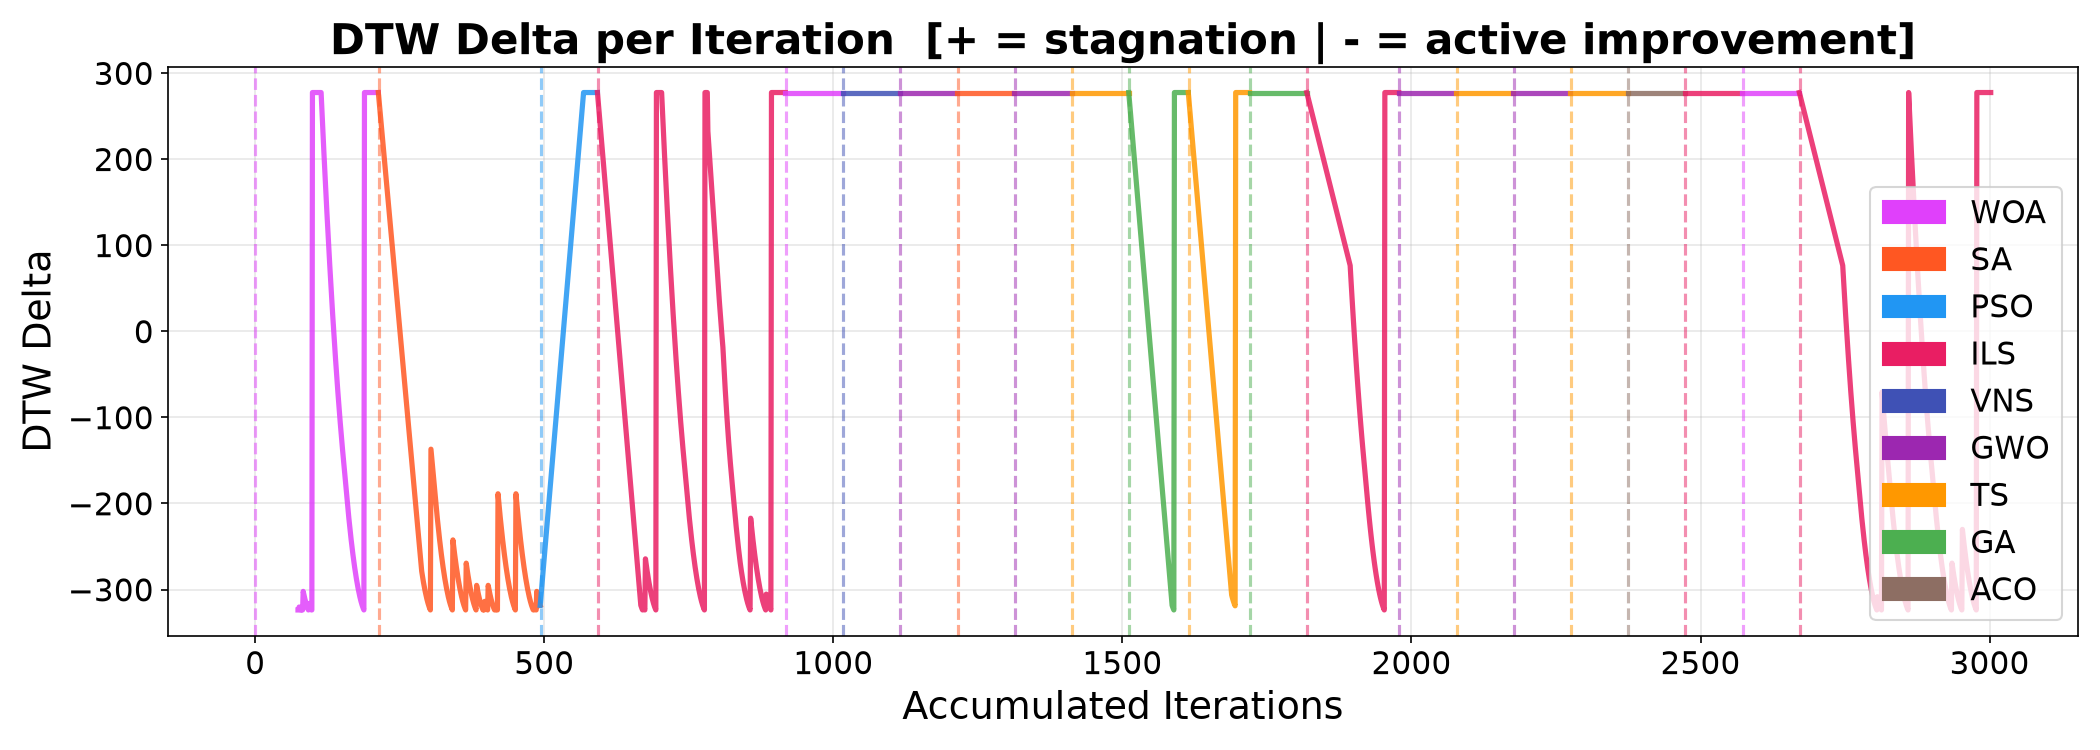
\includegraphics[width=0.32\textwidth]{imagenes_paper/mkp_dtw_3k_mknapcb6_delta.png}}
\caption{Diagnostic suite for instance \textbf{mknapcb6} ($n=500$, $m=10$) under the DTW framework with $T_{\max}=3{,}000$: (a)~final-fitness distribution over $N=31$ runs; (b)~convergence trajectory of the best run; (c)~elastic warping profile $\Delta$.}
\label{fig:mkp-best-cb6}
\end{figure}

% --- mknapcb7: DTW, 3,000 iterations ---
\begin{figure}[htbp]
\centering
\subfloat[Metaheuristic comparison.]{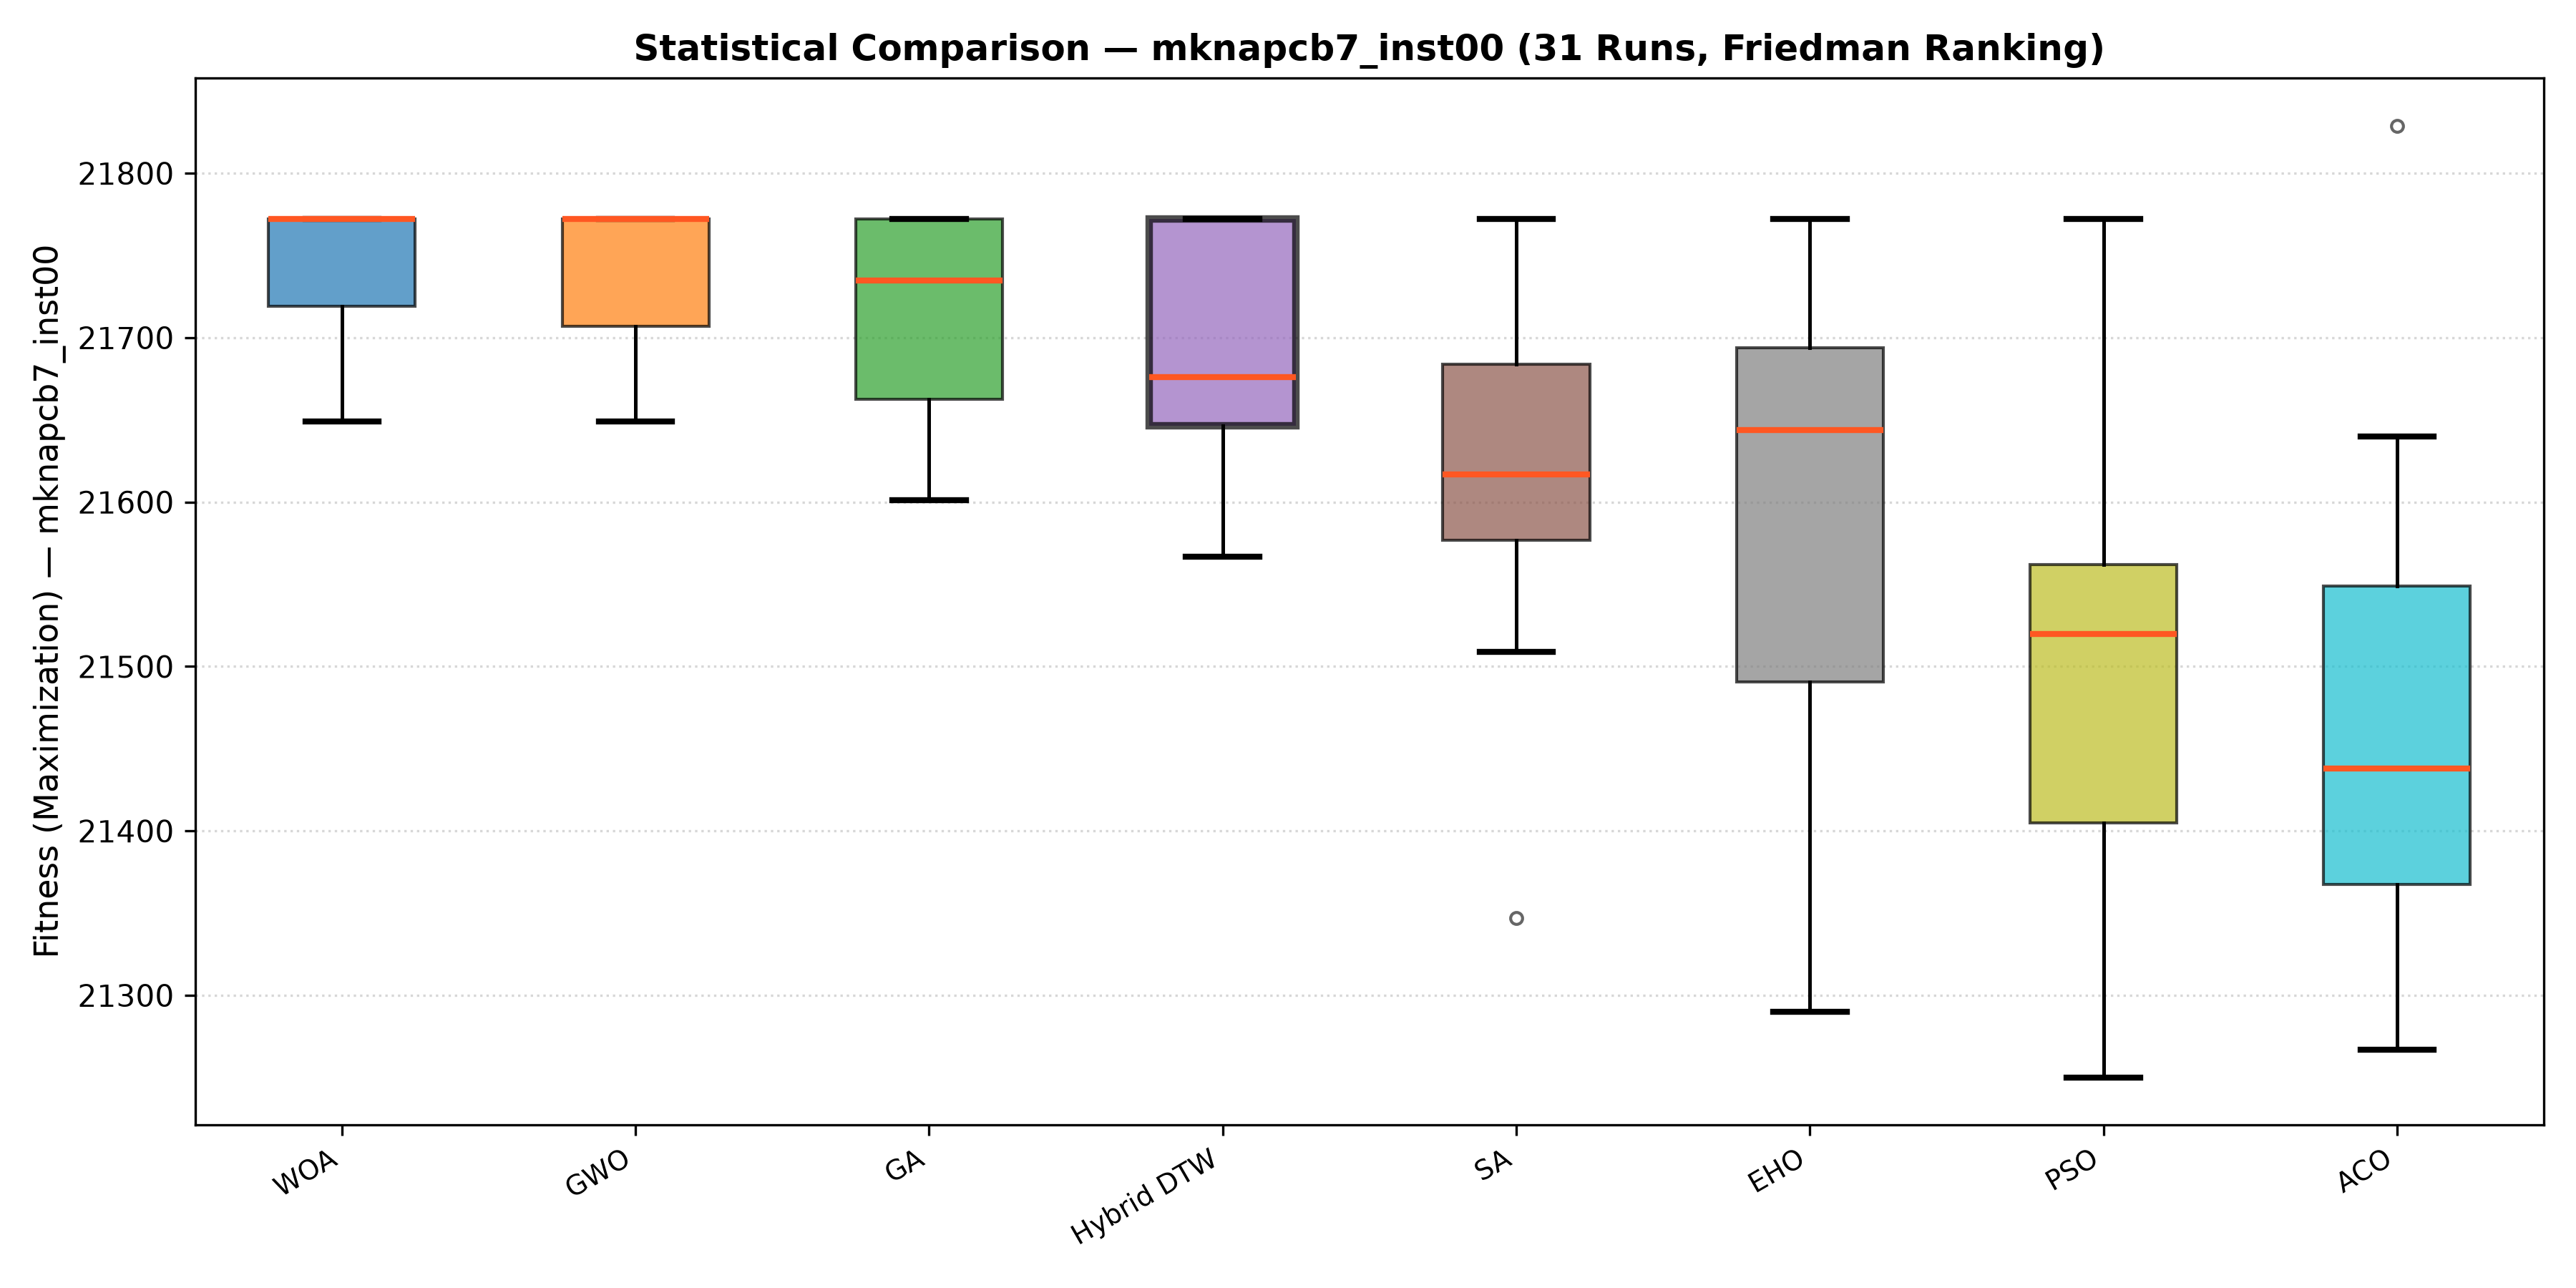
\includegraphics[width=0.32\textwidth]{imagenes_paper/mkp_dtw_3k_mknapcb7_comparativo_mh.png}}\hfill
\subfloat[Best-run convergence.]{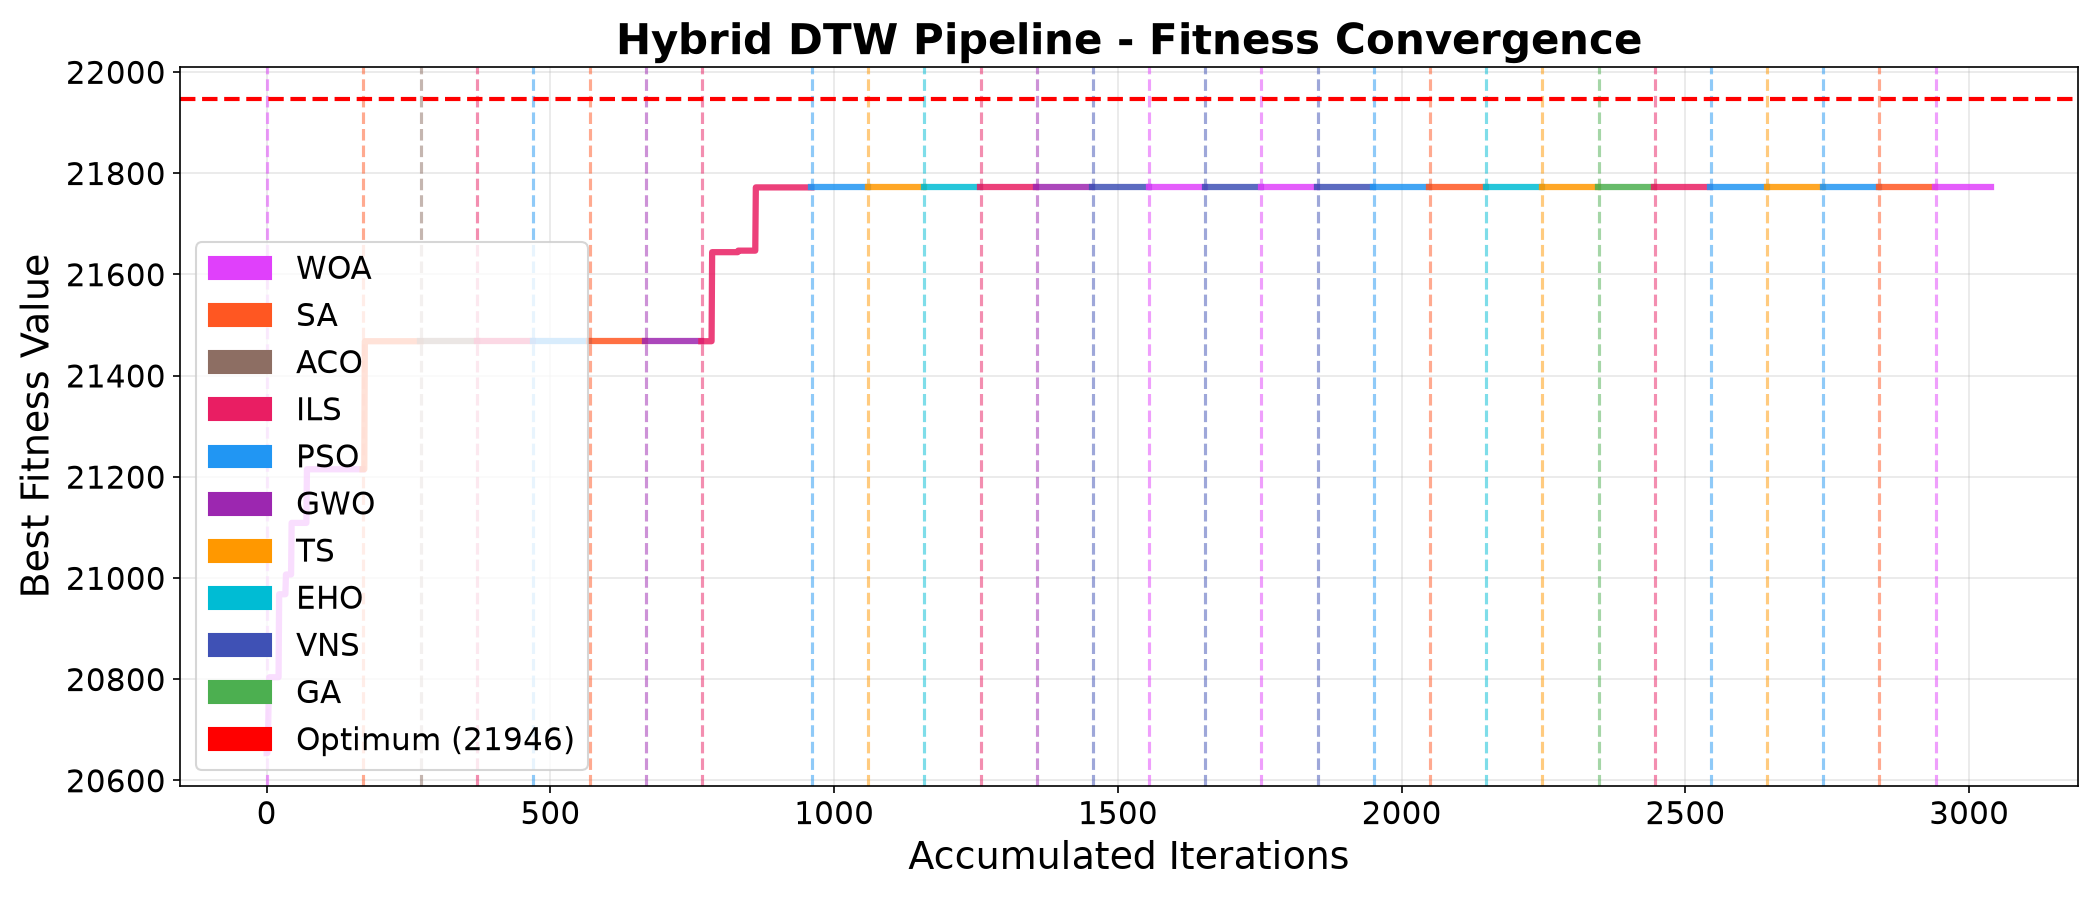
\includegraphics[width=0.32\textwidth]{imagenes_paper/mkp_dtw_3k_mknapcb7_convergencia.png}}\hfill
\subfloat[Elastic metric $\Delta=D_1-D_2$.]{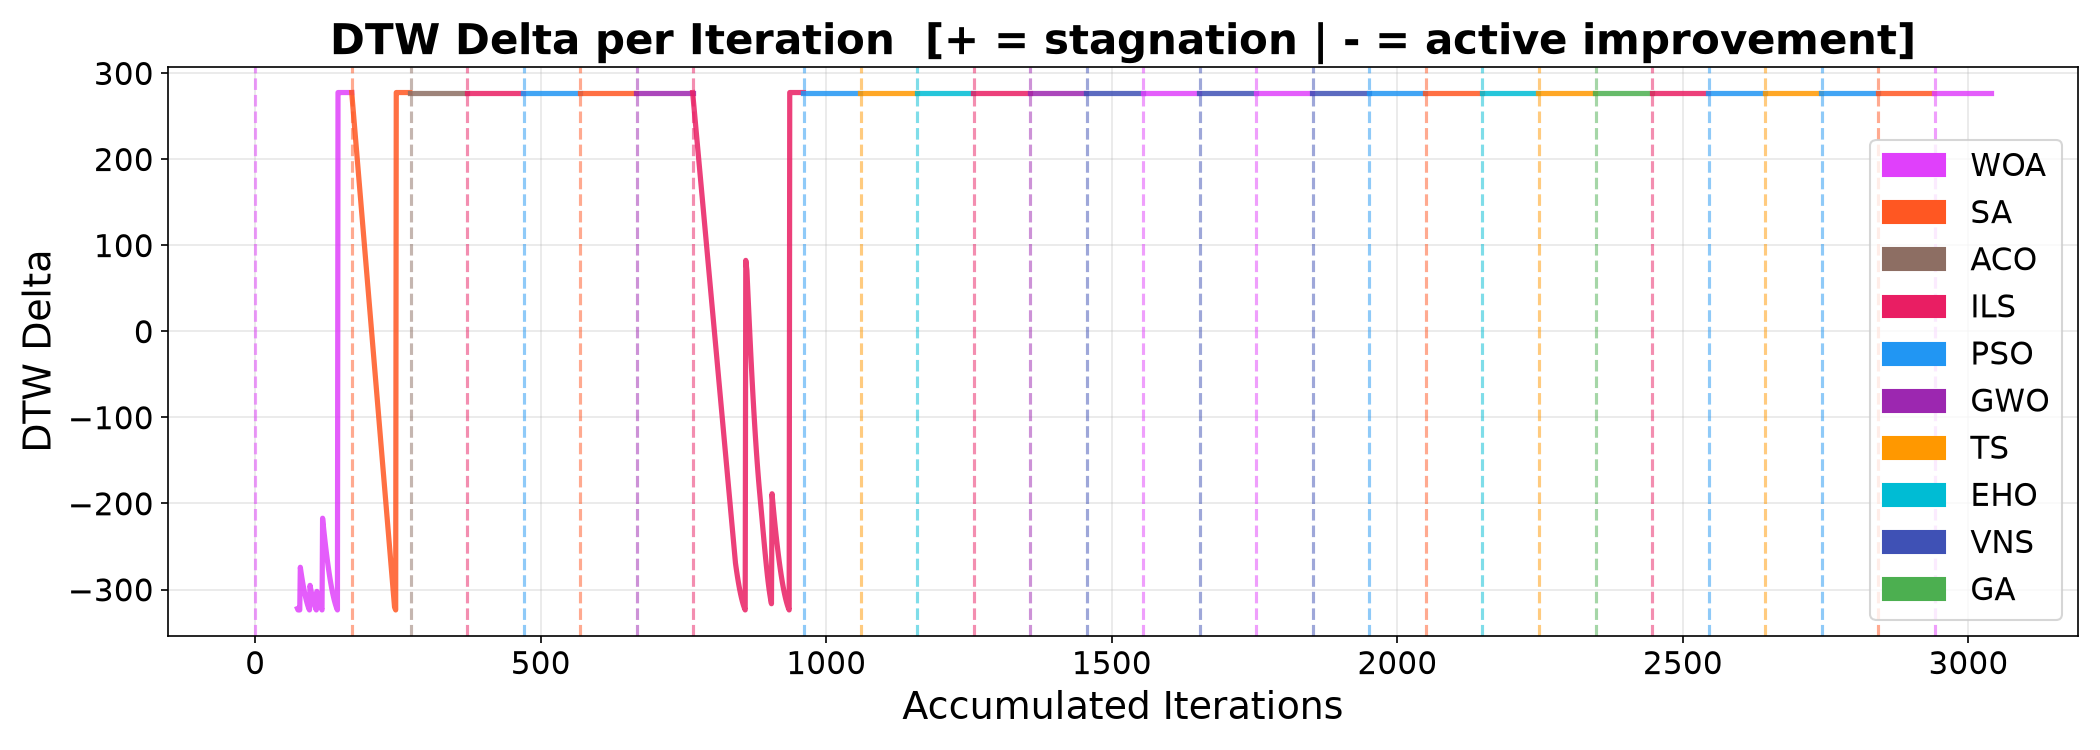
\includegraphics[width=0.32\textwidth]{imagenes_paper/mkp_dtw_3k_mknapcb7_delta.png}}
\caption{Diagnostic suite for instance \textbf{mknapcb7} ($n=100$, $m=30$) under the DTW framework with $T_{\max}=3{,}000$: (a)~final-fitness distribution over $N=31$ runs; (b)~convergence trajectory of the best run; (c)~elastic warping profile $\Delta$.}
\label{fig:mkp-best-cb7}
\end{figure}

% --- mknapcb8: DTW, 3,000 iterations ---
\begin{figure}[htbp]
\centering
\subfloat[Metaheuristic comparison.]{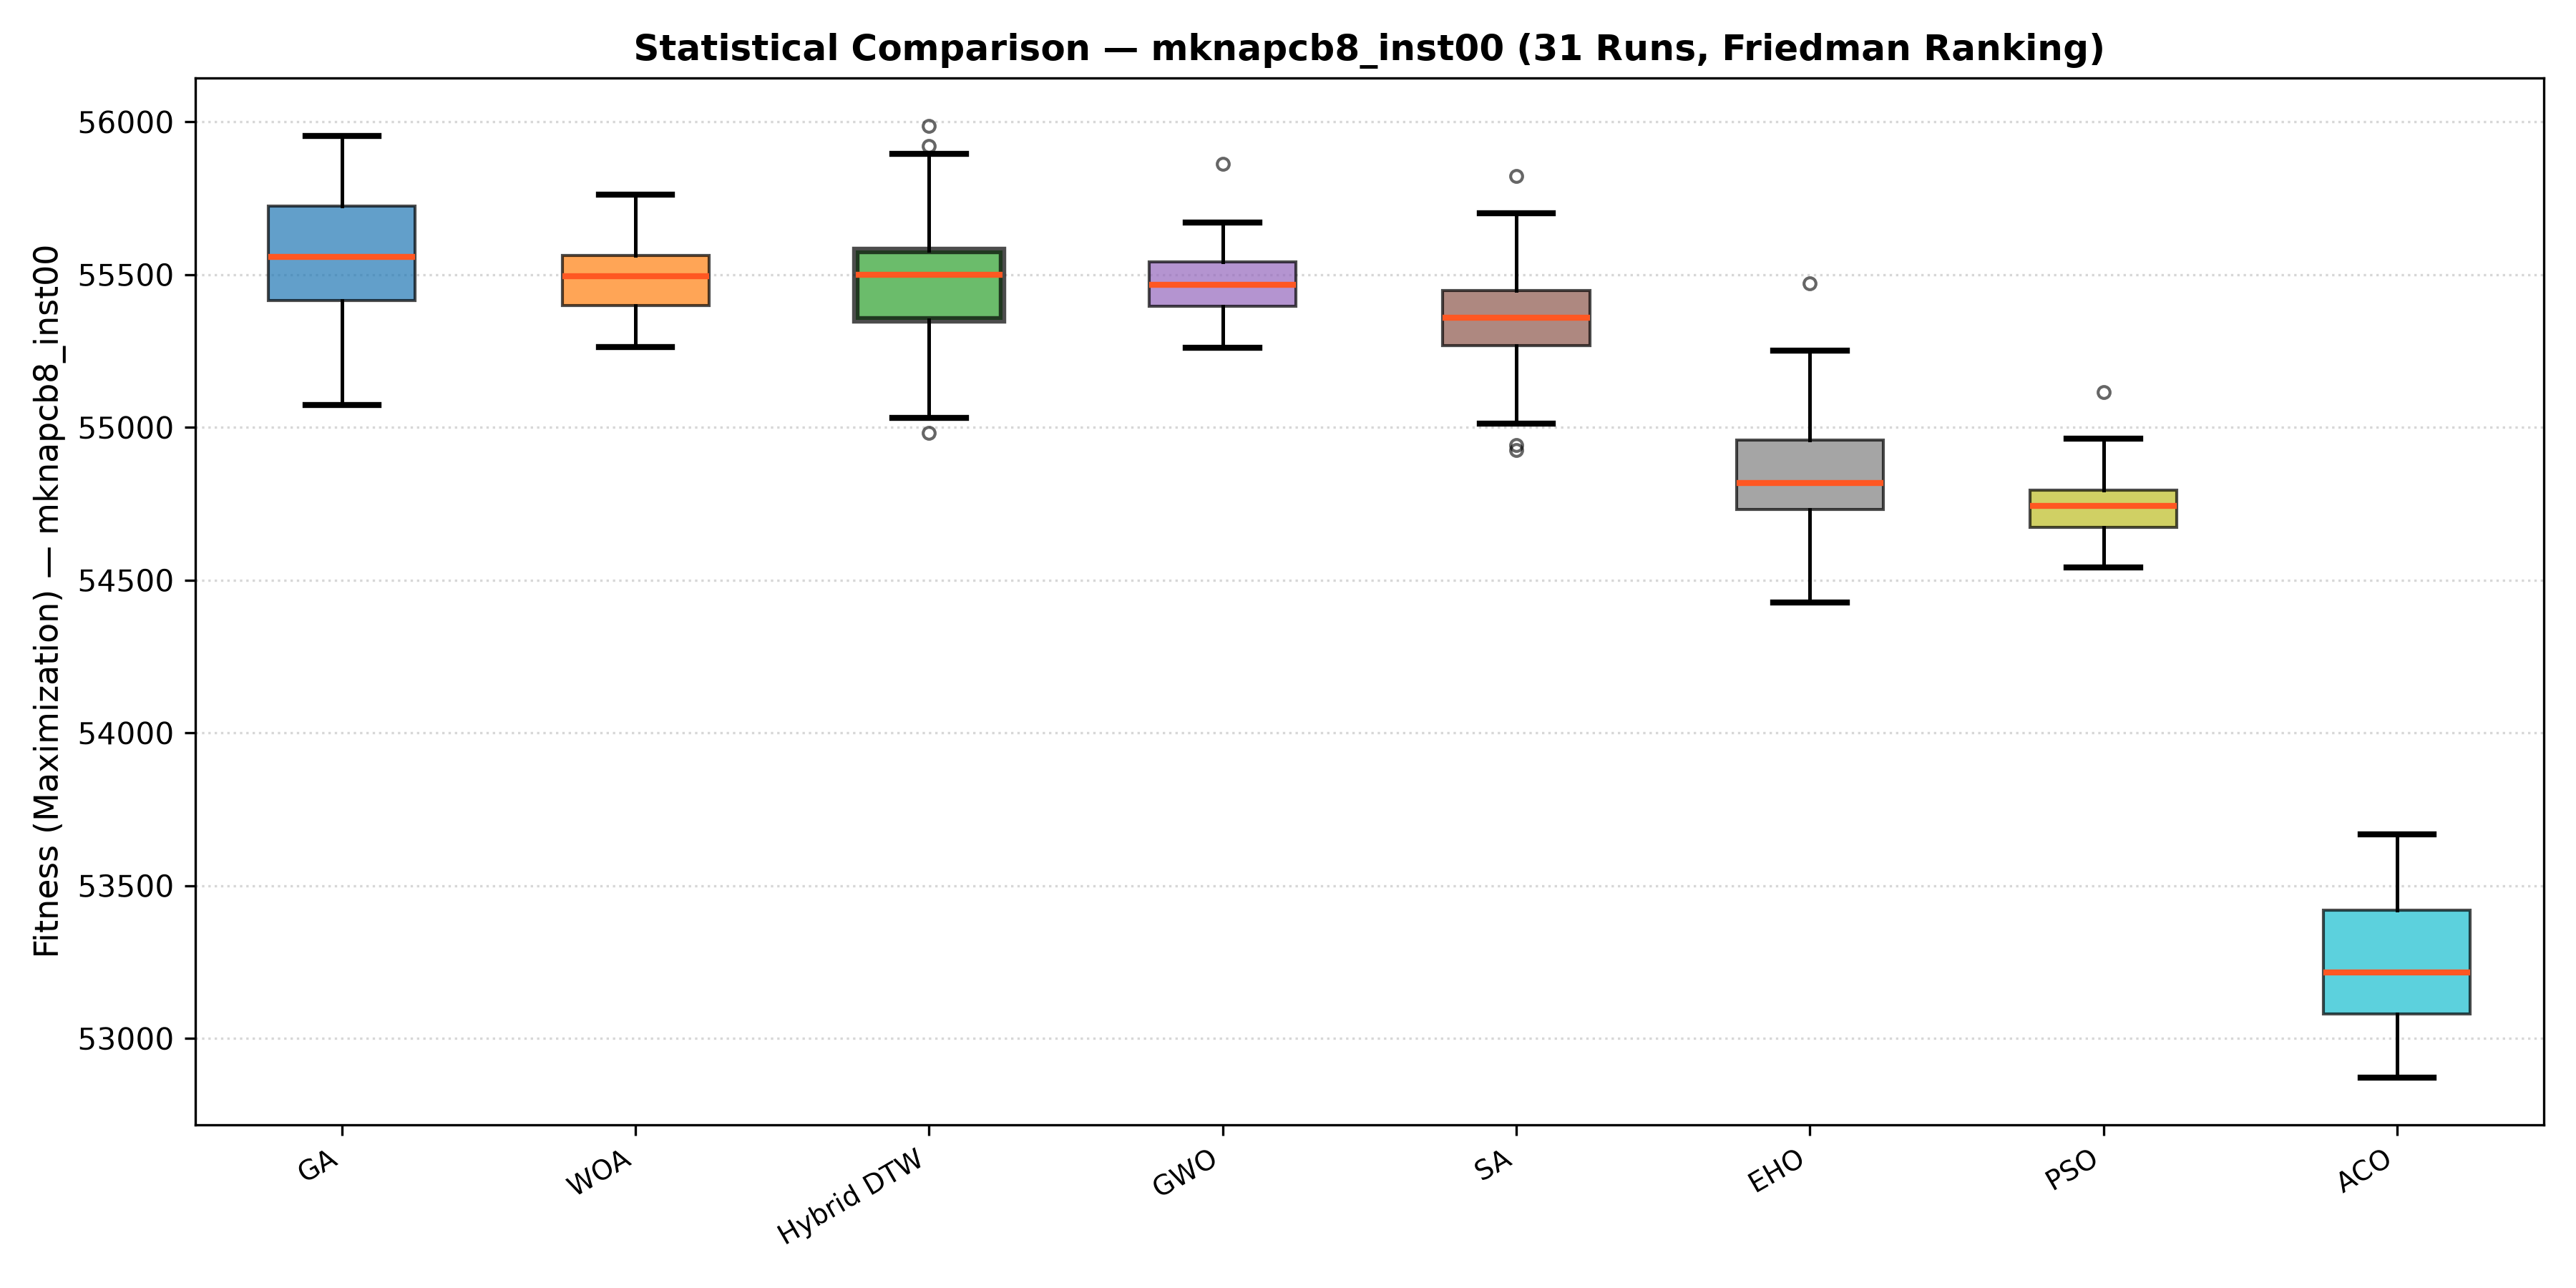
\includegraphics[width=0.32\textwidth]{imagenes_paper/mkp_dtw_3k_mknapcb8_comparativo_mh.png}}\hfill
\subfloat[Best-run convergence.]{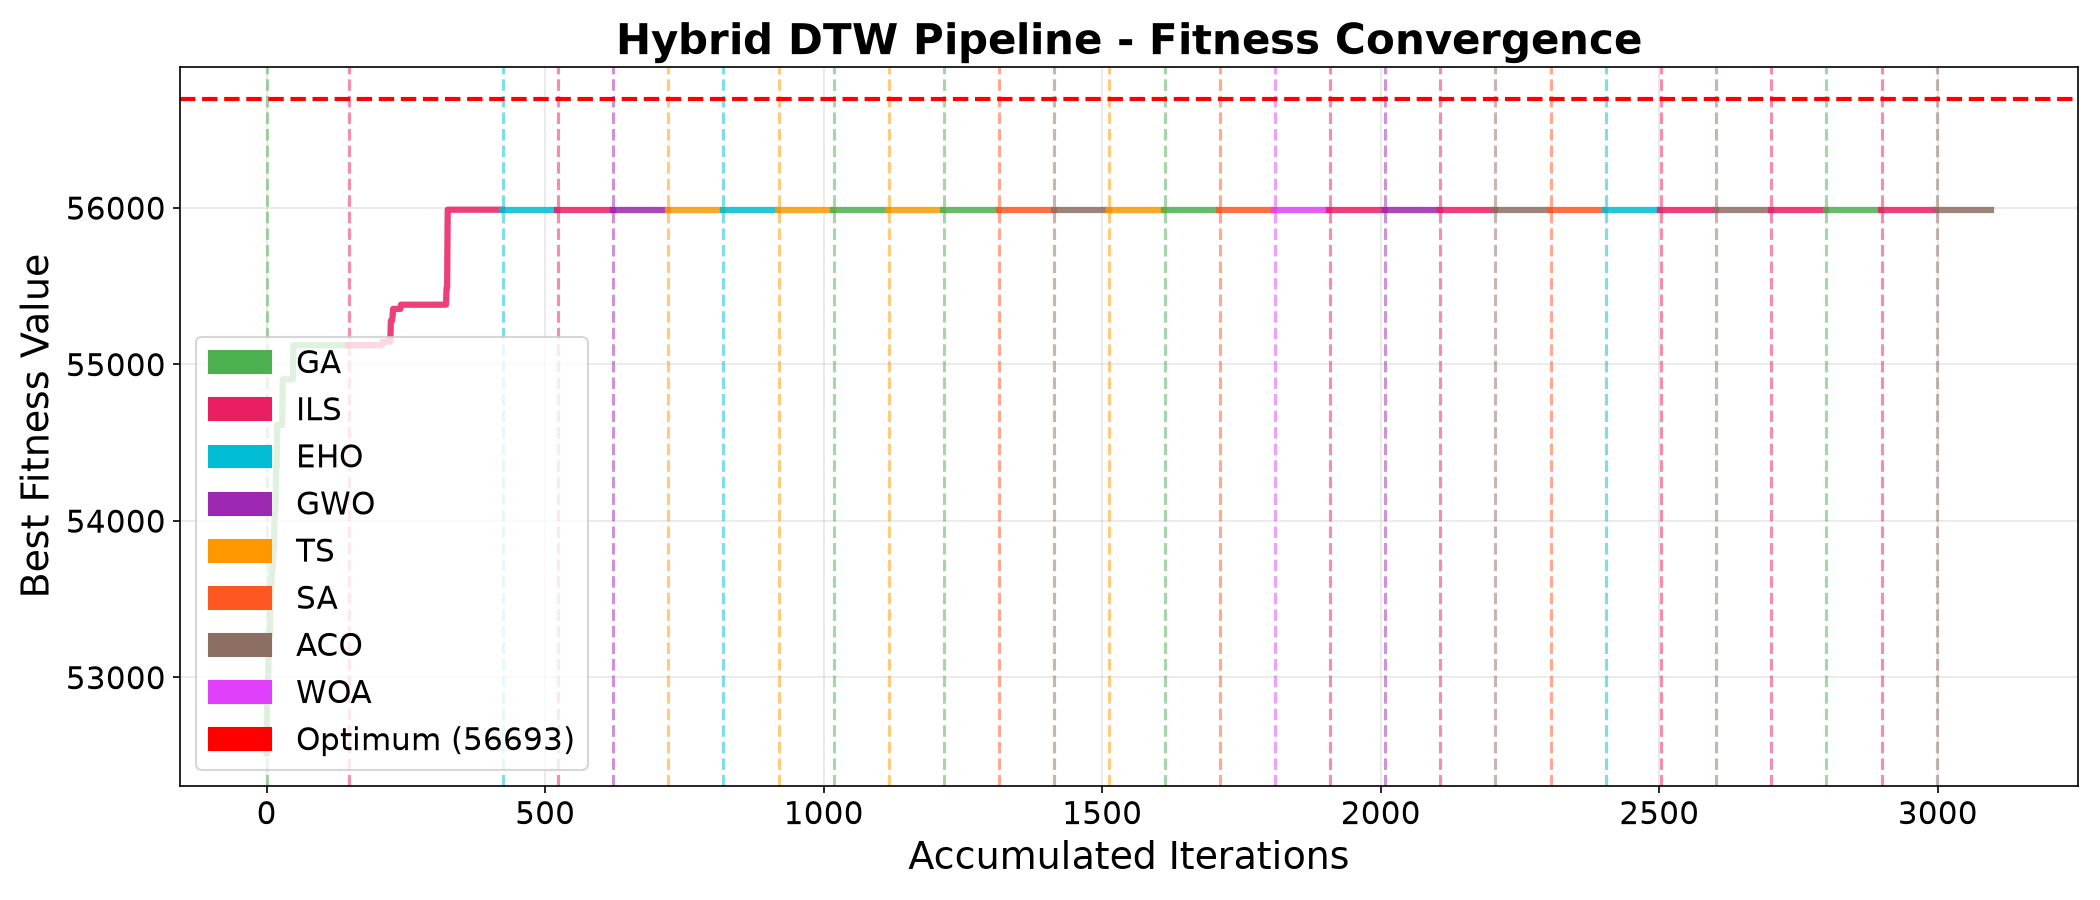
\includegraphics[width=0.32\textwidth]{imagenes_paper/mkp_dtw_3k_mknapcb8_convergencia.png}}\hfill
\subfloat[Elastic metric $\Delta=D_1-D_2$.]{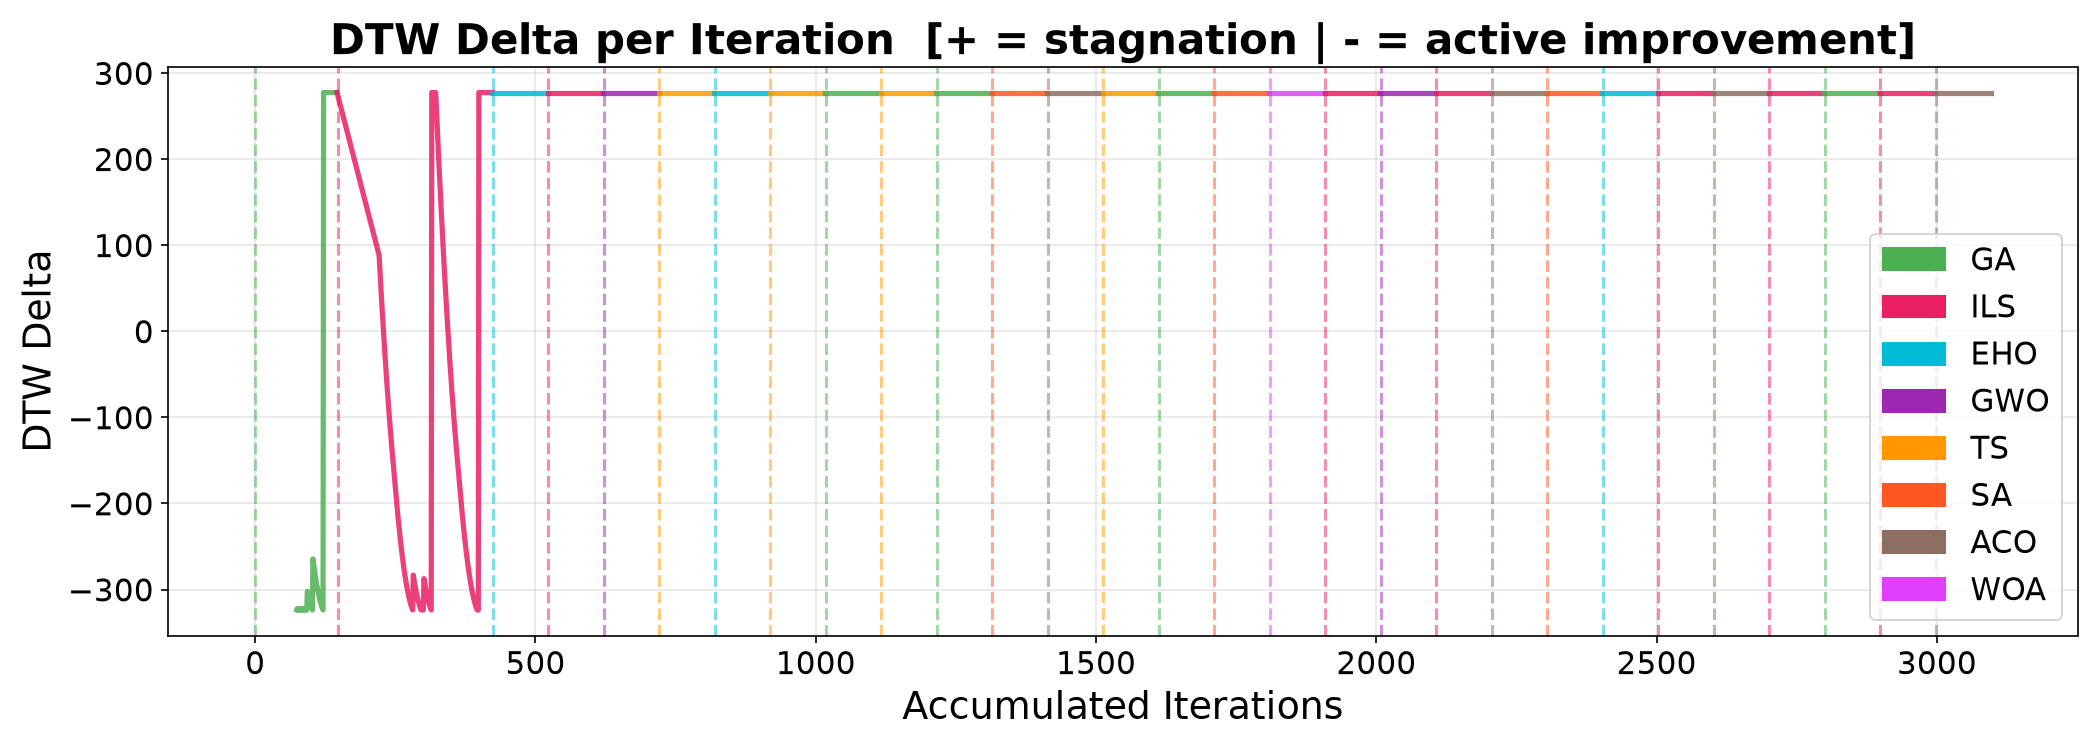
\includegraphics[width=0.32\textwidth]{imagenes_paper/mkp_dtw_3k_mknapcb8_delta.png}}
\caption{Diagnostic suite for instance \textbf{mknapcb8} ($n=250$, $m=30$) under the DTW framework with $T_{\max}=3{,}000$: (a)~final-fitness distribution over $N=31$ runs; (b)~convergence trajectory of the best run; (c)~elastic warping profile $\Delta$.}
\label{fig:mkp-best-cb8}
\end{figure}

% --- mknapcb9: DDTW, 3,000 iterations ---
\begin{figure}[htbp]
\centering
\subfloat[Metaheuristic comparison.]{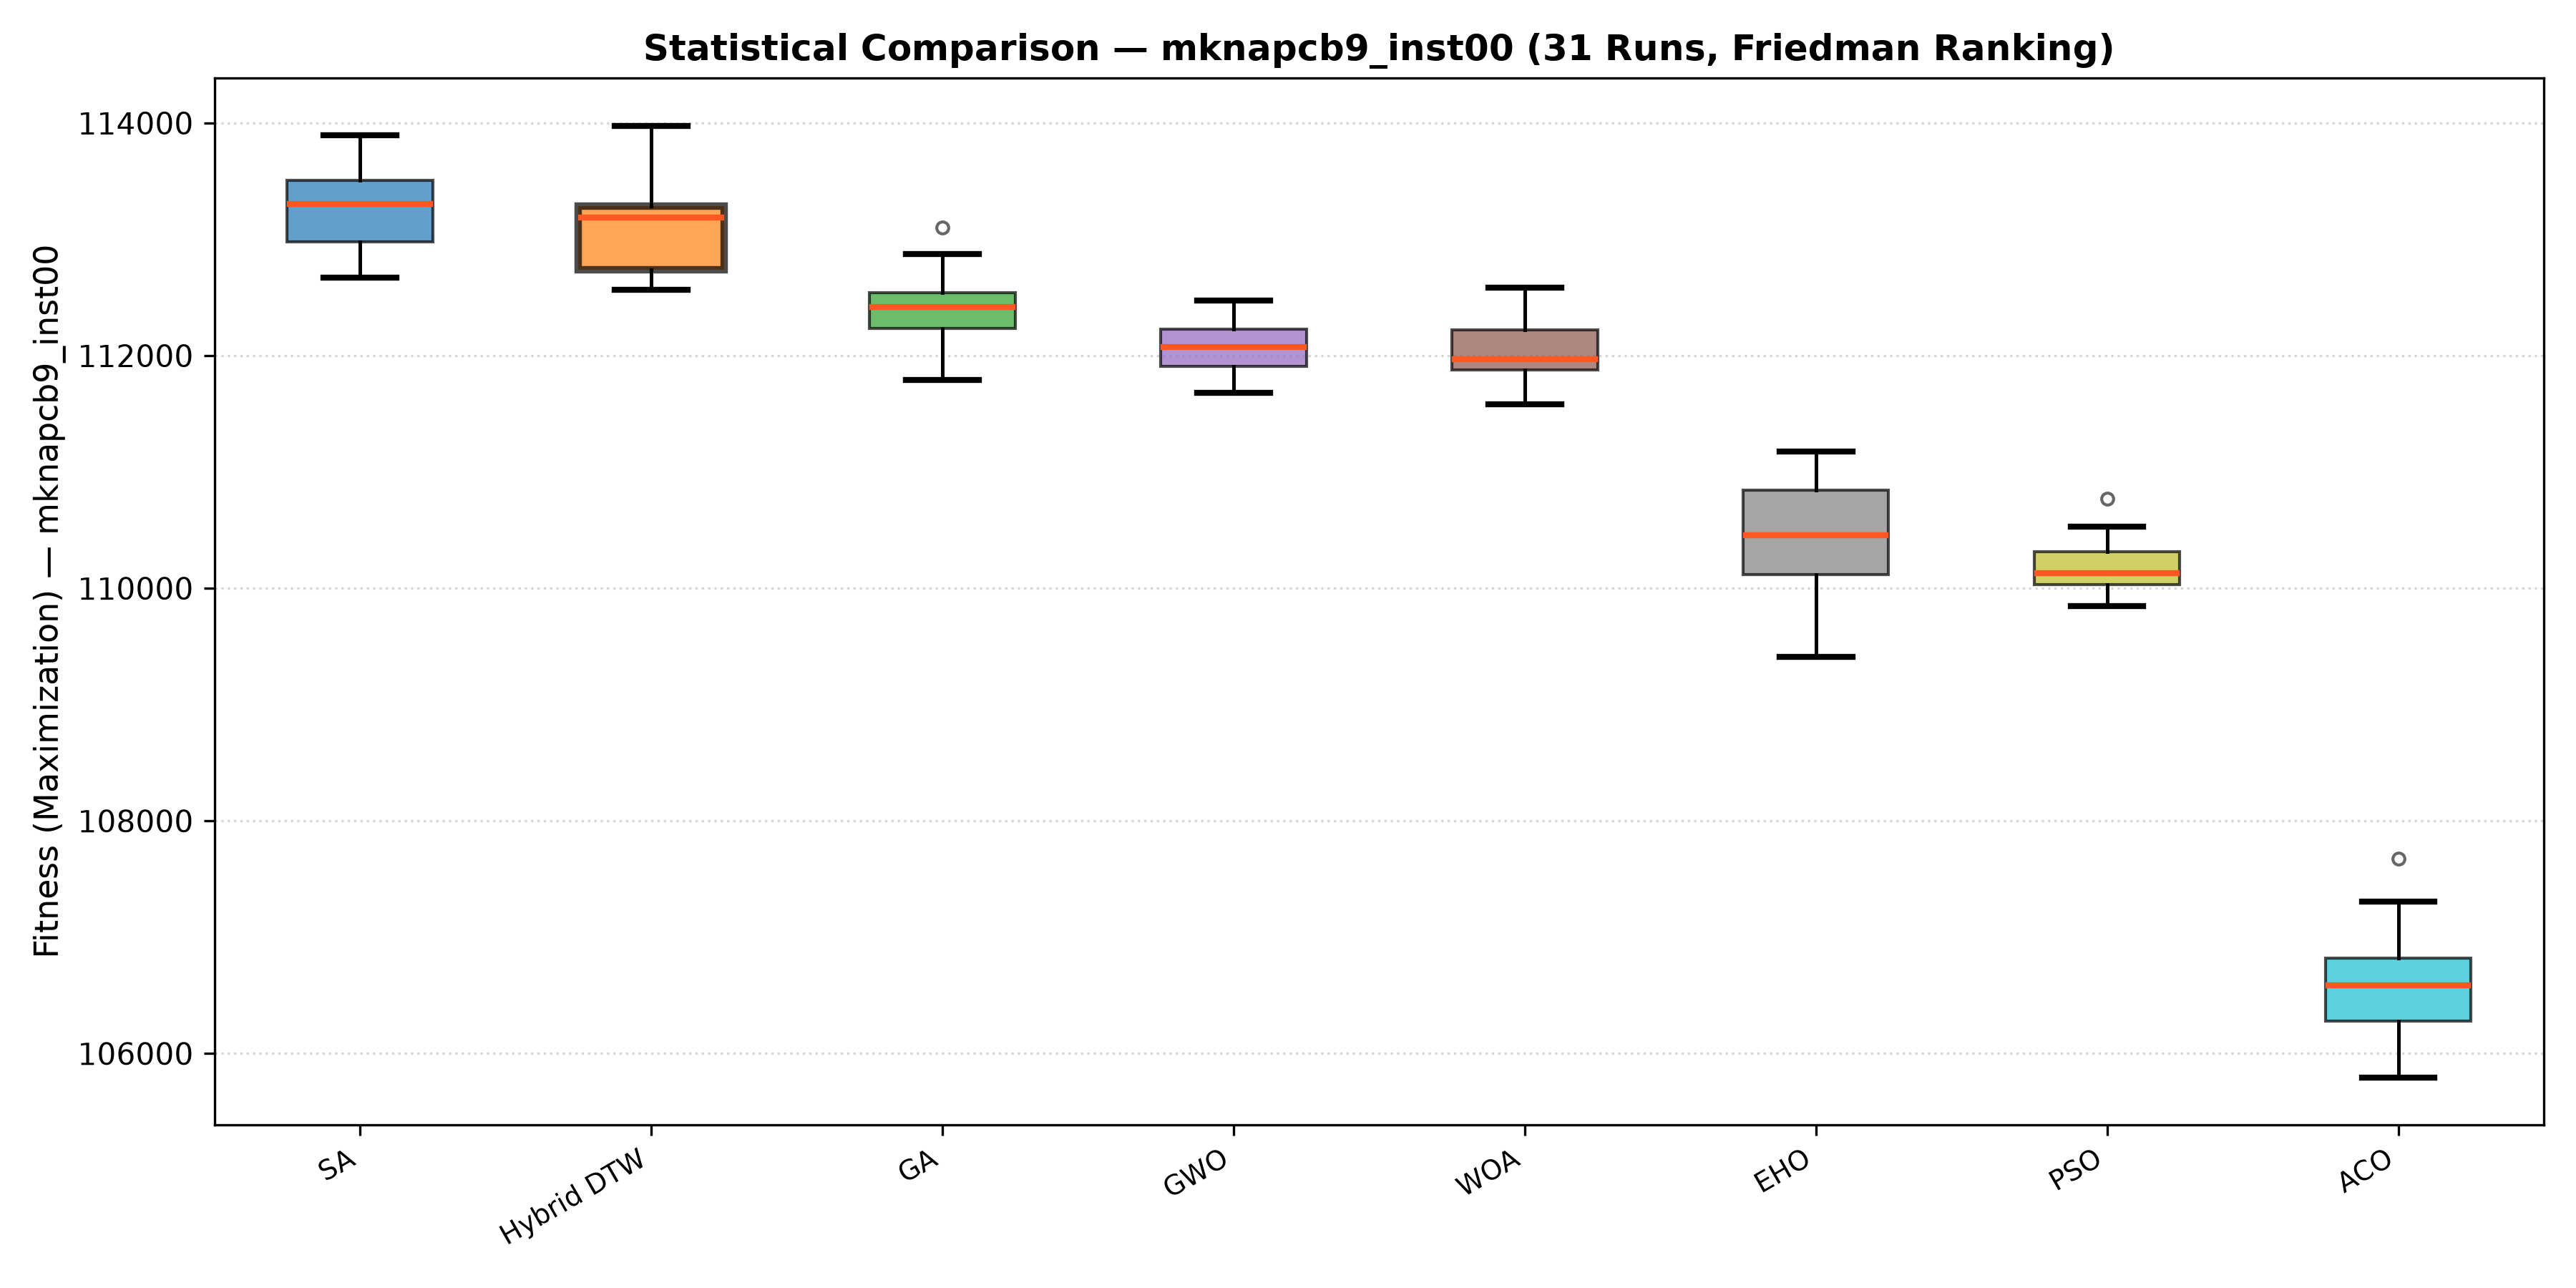
\includegraphics[width=0.32\textwidth]{imagenes_paper/mkp_ddtw_3k_mknapcb9_comparativo_mh.png}}\hfill
\subfloat[Best-run convergence.]{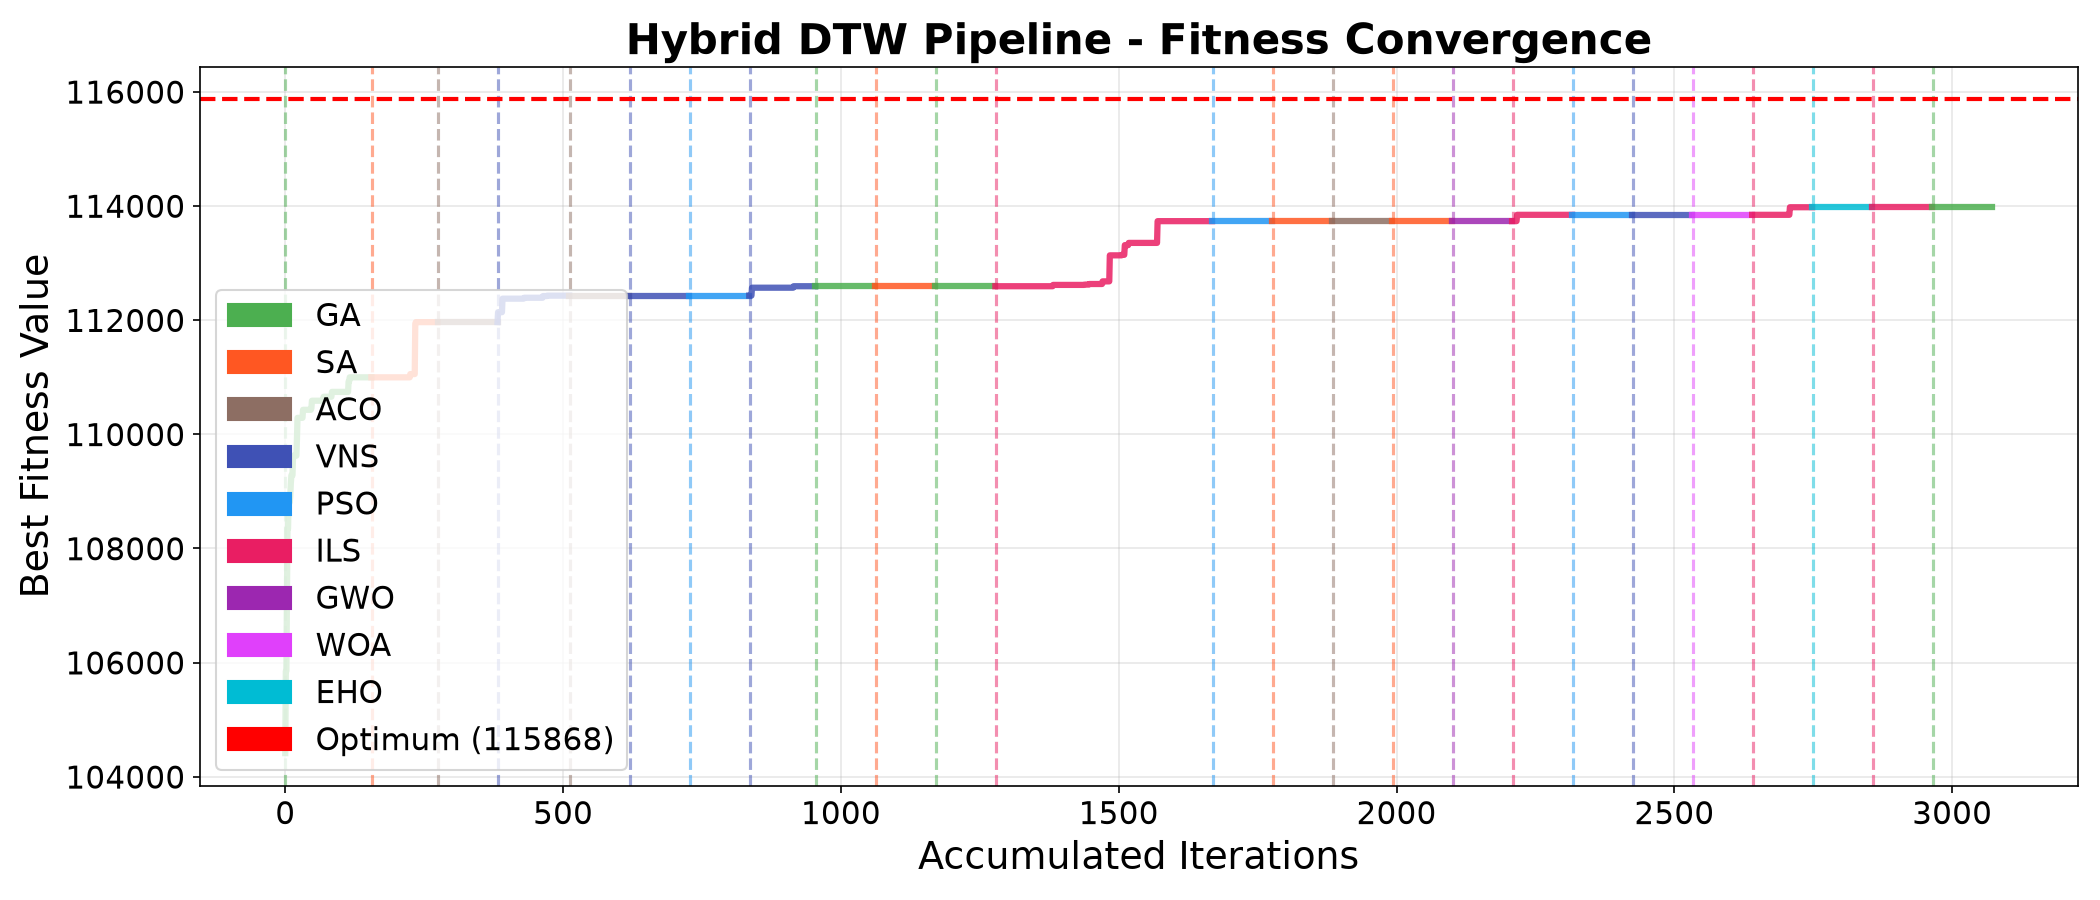
\includegraphics[width=0.32\textwidth]{imagenes_paper/mkp_ddtw_3k_mknapcb9_convergencia.png}}\hfill
\subfloat[Elastic metric $\Delta=D_1-D_2$.]{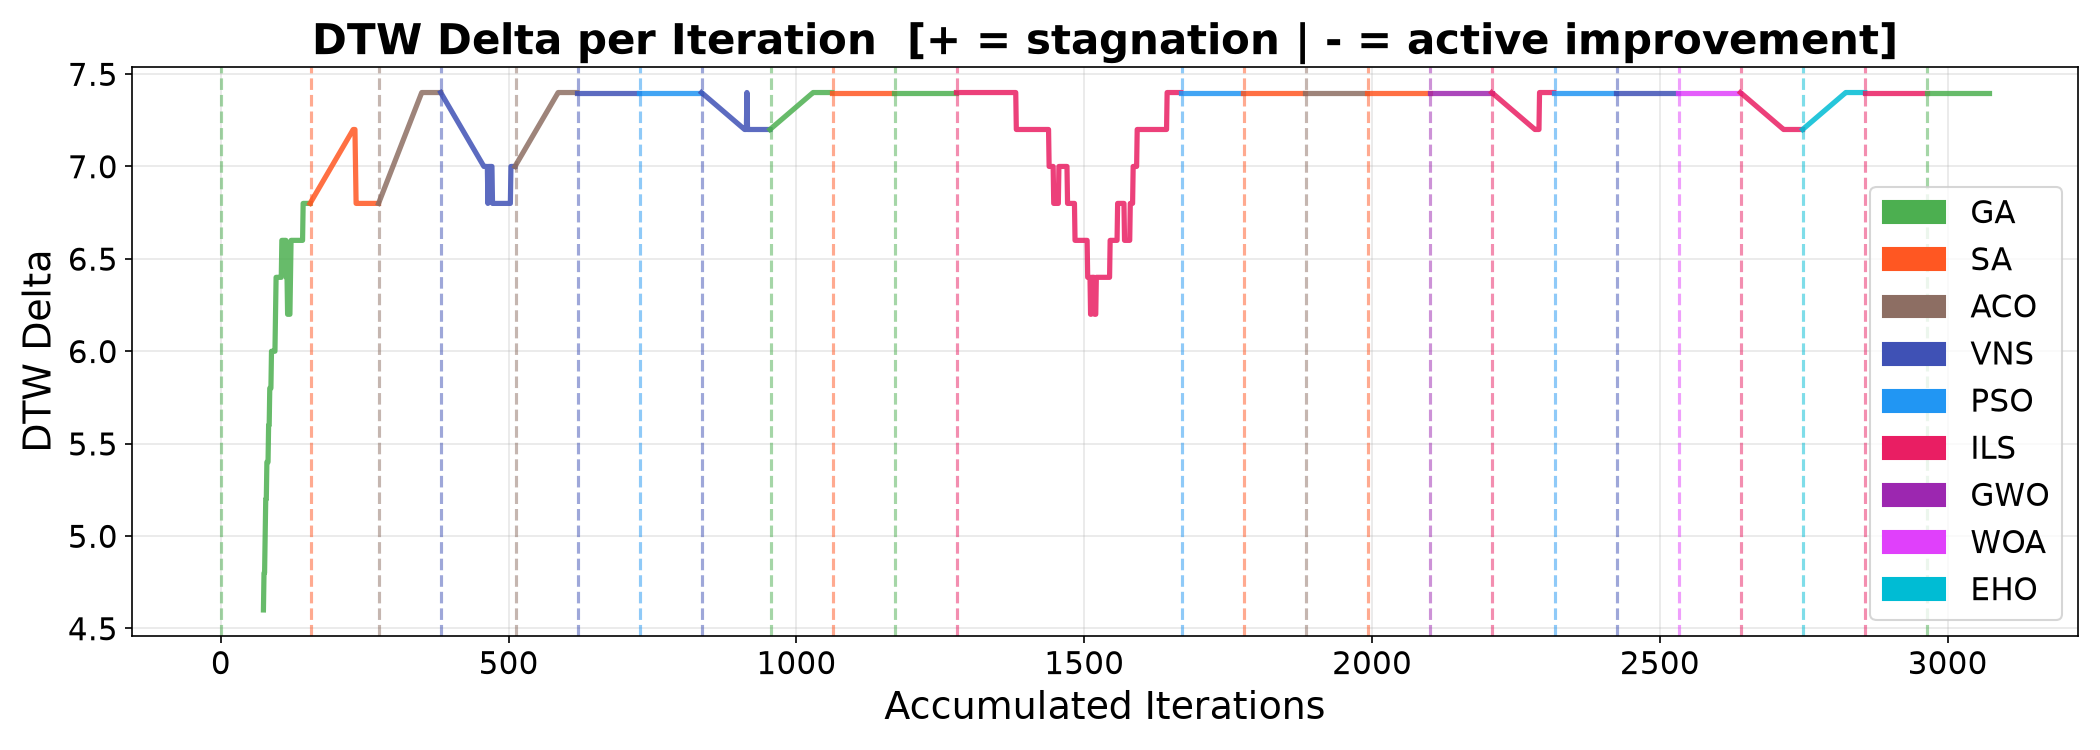
\includegraphics[width=0.32\textwidth]{imagenes_paper/mkp_ddtw_3k_mknapcb9_delta.png}}
\caption{Diagnostic suite for instance \textbf{mknapcb9} ($n=500$, $m=30$) under the DDTW framework with $T_{\max}=3{,}000$: (a)~final-fitness distribution over $N=31$ runs; (b)~convergence trajectory of the best run; (c)~elastic warping profile $\Delta$.}
\label{fig:mkp-best-cb9}
\end{figure}
